%% to be called from the project root: file paths are relative to that

\documentclass[a4paper,12pt]{book}

\usepackage[svgnames]{xcolor}
\usepackage{lipsum}  %% dev
\usepackage{dpfloat}
\usepackage{amsmath}
\usepackage{amssymb}
\usepackage{amsthm}
\usepackage{mathrsfs}
\usepackage{xparse}  %% required by physics
\usepackage{physics}
\usepackage{breqn}
\usepackage{bbm}
\usepackage[utf8]{inputenc}
\usepackage{mathtools}
\usepackage[super]{nth}
\usepackage[inline]{enumitem}
\usepackage{graphicx}
\usepackage{subcaption} % https://tex.stackexchange.com/a/43996 + https://tex.stackexchange.com/a/165730
  \captionsetup{subrefformat=parens}
\usepackage{color}

\usepackage[a4paper,lmargin=4cm]{geometry}

\usepackage{multirow}
\usepackage{fancyhdr}
\pagestyle{fancy}  %% prevent long section titles from overflowing page headers
  \fancyhf{}
  \fancyhead[LE]{\thepage}
  \fancyhead[RE]{\textit{\nouppercase{\leftmark}}}
  \fancyhead[LO]{\textit{\nouppercase{\rightmark}}}
  \fancyhead[RO]{\thepage}
\fancypagestyle{nomark}{%
  \fancyhf{}
  \fancyhead[LE]{\thepage}
  \fancyhead[RE]{}
  \fancyhead[LO]{}
  \fancyhead[RO]{\thepage}
}
\setlength{\headheight}{14.5pt}  %% prevent fancyhead Warning.

% https://tex.stackexchange.com/a/1557
% https://tex.stackexchange.com/a/176939
\usepackage[safeinputenc,style=authoryear-icomp,mincitenames=1,maxcitenames=2,uniquelist=minyear,maxbibnames=7,backend=biber]{biblatex}
%\usepackage[safeinputenc,uniquelist=minyear,maxbibnames=7,backend=biber]{biblatex}
\usepackage{environ}
\usepackage{csquotes}
\usepackage{epigraph}
  \setlength{\epigraphwidth}{.66\textwidth}
  \renewcommand{\epigraphsize}{\small}
  \setlength{\epigraphrule}{0.005pt}
  \setlength{\beforeepigraphskip}{.8\baselineskip}
  \setlength{\afterepigraphskip}{1.2\baselineskip}
\usepackage{fancyvrb}
  \fvset{
    frame = single,
    rulecolor=\color{lightgray}
  }
\usepackage{footnote}
%
% Ways to avoid "random" vertical space between paragraphs
% https://tex.stackexchange.com/a/36429
\raggedbottom
\usepackage[bottom]{footmisc}
%
\usepackage{listings}
  \lstset{
    frame = single,
    rulecolor=\color{lightgray},
    basicstyle=\setstretch{1.2}\scriptsize\ttfamily,
    commentstyle=\color{gray},
    keywordstyle=\color{blue},
    stringstyle=\color{red},
    fancyvrb=true,
    breaklines=true,
    aboveskip=1.1em,
    belowskip=0.4em,
    %identifierstyle=\color{green!40!black}
  }
\usepackage{setspace}
\usepackage{etoolbox}
\usepackage[  %% be (almost) the last -- https://tex.stackexchange.com/a/326953
  %% pdfusetitle would not render the ket <1| correctly -- title is a plain text
  pdftitle={It's |1> o'clock -- Relational Time and Applications},
  colorlinks
]{hyperref}
  \hypersetup{
    linkcolor = DarkRed,
    citecolor = Green,
    urlcolor  = DarkBlue
  }

% https://tex.stackexchange.com/a/65547
\usepackage{bookmark}

% "dev only"
\ifdev
  % \usepackage[breakable,skins]{tcolorbox}
  % \definecolor{tcbcolback} {HTML}{EEEEFF}
  % \definecolor{tcbcolframe}{HTML}{4444BB}
  % \tcbset{
  %   colback=tcbcolback, colframe=tcbcolframe,
  %   breakable, enhanced jigsaw,
  %   parbox=false, before upper={%
  %     \setlength{\parskip}{0.666em}%
  %     \setlength{\parindent}{0pt}%
  %     \setstretch{1.2}%
  %   }
  % }

  % https://tex.stackexchange.com/a/53252
  \pdfcompresslevel=0
  \pdfobjcompresslevel=0
\fi

%%%%

%% Theorem-like environments

%% http://www.maths.tcd.ie/~dwilkins/LaTeXPrimer/Theorems.html
%% https://www.sharelatex.com/learn/Theorems_and_proofs
%% http://tex.stackexchange.com/a/46262
\newtheorem{theorem}{Theorem}[section]
\newtheorem{lemma}[theorem]{Lemma}
\newtheorem{proposition}[theorem]{Proposition}
\newtheorem{corollary}{Corollary}[theorem]
\newtheorem{remark}{Remark}[section]
\newcommand{\remarkautorefname}{Remark}

%% Adapted from https://tex.stackexchange.com/q/45817
\theoremstyle{definition}
\newtheorem{definition}{Definition}[section]
\newtheorem{axiom}{Axiom}[section]
\newtheorem{conjecture}{Conjecture}[section]
\newtheorem{example}{Example}[section]

%%%%

\newcommand{\ch}{{c.}\:}             % chapter in bib citations
\newcommand{\s}{{s.}\:}              % section in bib citations
\newcommand{\citeplace}[1]{{#1}\:}   % ``any'' in bib citations  e.g. \cite[\citeplace{handout} 2]{Webber_notes}

\newcommand{\term}[1]{\emph{#1}}
\newcommand{\idop}{\mathbbm{1}}           % Identity operator
\newcommand{\hilb}[1]{\mathcal{#1}}       % Hilbert space
\newcommand{\setof}[1]{\left\{#1\right\}}
\newcommand{\ox}{\otimes}
\newcommand{\transpose}{\top}

%% Allows better formatting than \underset
%% https://tex.stackexchange.com/a/130553
\DeclareMathOperator*{\repr}{\,\equiv\,}      % represented in a basis, or "has components..."

\renewcommand{\op}{\hat}                  % overwriting physics \op = \ketbra
%\renewcommand{\op}{}                      % overwriting physics \op = \ketbra
\newcommand{\eqbydef}{\coloneqq}
%\newcommand{\eqbydef}{\triangleq}
\newcommand{\superop}{\mathcal}

\newcommand{\dket}[1]{\left.\left| #1 \right\rangle\right\rangle}
\newcommand{\Dket}[1]{\left.\left| #1 \right\rangle\!\right\rangle}
\newcommand{\dbra}[1]{\left\langle\left\langle #1 \right|\right.}
\newcommand{\Dbra}[1]{\left\langle\!\left\langle #1 \right|\right.}
\newcommand{\dbraket}[2]{\left\langle\left\langle #1 \middle| #2 \right\rangle\right.\!}
\newcommand{\bradket}[2]{\!\left.\left\langle #1 \middle| #2 \right\rangle\right\rangle}
\newcommand{\braDket}[2]{\!\left.\left\langle #1 \middle| #2 \right\rangle\!\right\rangle}
\newcommand{\dbradket}[2]{\left\langle\left\langle #1 \middle| #2 \right\rangle\right\rangle}
\newcommand{\dketdbra}[2]{\dket{#1}\dbra{#2}}

%% smaller than \quad but still quite larger than \;
\newcommand{\kuad}[0]{\:\:\,}

\newcommand{\pwspace}{\hilb{H}_T \ox \hilb{H}_S}

\NewEnviron{eqsplit}{\begin{equation}\begin{split}\BODY\end{split}\end{equation}}
\NewEnviron{eqsplit*}{\begin{equation*}\begin{split}\BODY\end{split}\end{equation*}}

% Imaginary unit (not used much this way here though)
% https://tex.stackexchange.com/a/303698
\newcommand{\iu}{\mathrm{i}\mkern1mu}
\newcommand{\E}{\mathrm{e}}

% Functions
% Heaviside function
\newcommand{\Hvsd}[1]{\Theta\left(#1\right)}

%\newcommand{\nullvector}{\underline{0}}
\newcommand{\nullvector}{0}


\renewcommand{\arraystretch}{1.6}

% https://tex.stackexchange.com/a/325704
\AtBeginEnvironment{quote}{\singlespace\vspace{-\topsep}}
\AtEndEnvironment{quote}{\vspace{-\topsep}\endsinglespace}

\author{Guido De Rosa \\ \small\tt{gderosa@umail.ucc.ie}}
\title{It's $\ket{1}$ o'clock -- Relational Time and Applications}

\addbibresource{bib/main.bib}
\addbibresource{bib/comp.bib}
\addbibresource{bib/misc.bib}
% For peer-reviewed articles, in general there is a DOI which is detailed enough,
% while only some entries have issn fields, essentially out of a copypaste -
% See also https://tex.stackexchange.com/a/32933.
\AtEveryBibitem{
  \clearfield{issn}
  \clearfield{month}
}


\begin{document}

\frontmatter

%% Vertical spacing, par. skip, indent... possibly to be readjusted in different parts of the document?
%% (which is why they're not in preamble.tex).
% \setstretch{1.4}
% \setlength{\parindent}{4ex}
%
\onehalfspacing
\setlength{\parskip}{0.5ex}

\pagenumbering{alph}
\pdfbookmark[section]{Front}{front}
\thispagestyle{empty}

\newgeometry{hmargin=1in,vmargin=1in}

\begin{centering}

\textbf{NATIONAL UNIVERSITY OF IRELAND, CORK}

\vspace{1cm}


\includegraphics[width=0.333\linewidth]{img/ucc_logo.pdf}

\vspace{0.5in}

\Huge

{It's ${\ket{1}}$ o'clock -- Relational Time and Applications}

\vspace{0.25in}

\Large
by
\\
Guido De Rosa

\vspace{0.5in}

\large

Thesis submitted for the degree of\\
Master of Science

in the Department of Physics

\vspace{0.25in}

Supervisor: Dr. Andreas Ruschhaupt

Head of Department: Prof. John McInerney

\vspace{2cm}

\Large
2021

\end{centering}

\clearpage

\thispagestyle{empty}

\cleardoublepage

\restoregeometry


\pagenumbering{roman}
\maketitle

  {
    \hypersetup{
      linkcolor = .
    }

    % https://tex.stackexchange.com/a/65547
    \cleardoublepage
    \pdfbookmark[section]{\contentsname}{toc}
    \tableofcontents

    \cleardoublepage
    %\pdfbookmark[section]{\listfigurename}{lof}
    \listoffigures
    \addcontentsline{toc}{section}{\listfigurename}

    \cleardoublepage
    %\pdfbookmark[section]{\listtablename}{lot}
    \listoftables
    \addcontentsline{toc}{section}{\listtablename}
  }


\onehalfspacing

\chapter*{Declaration of Authorship}
\markboth{Declaration of Authorship}{Declaration of Authorship}  %% No ugly "Chapter 0".
\addcontentsline{toc}{section}{Declaration of Authorship}
This is to certify that the work I am submitting is my own and has not been
submitted for another degree, either at University College Cork or elsewhere. All
external references and sources are clearly acknowledged and identified within the
contents. I have read and understood the regulations of University College Cork
concerning plagiarism.

\chapter*{}

\vspace{2em}

\begin{flushright}\small
  If only \emph{Bob} could speak, he'd certainly thank \emph{Alice}.
\end{flushright}

\markboth{}{}

\chapter*{Acknowledgements}
\markboth{Acknowledgements}{Acknowledgements}  %% No ugly "Chapter 0".
\addcontentsline{toc}{section}{Acknowledgements}
{\it{\it%
I have been working towards a MSc.\;by Research in Physics
while continuing a full-time career as a software engineer and IT professional. 
I want to thank my colleagues, friends, and mentors,
for their encouragement and intellectual curiosity about this endeavour. 

I want to thank my family, friends, adored ones, back in Italy and beyond.
Thanks to all those who have supported this ideal journey.

This work comes after a series of interruptions, delays,
and the contradictions of an
an overly ambitious subject and some material difficulties:
a thesis about time that is running out of time\dots

Thanks to my fellow postgraduate students, one in particular with whom I have shared
an office, and long, fruitful conversations;
as well as the Research Staff, and our Senior Collaborator in a special way. 

Thanks to my Supervisor, for his patience, among other qualities, which I have sometimes, and admittedly, challenged.

Also thanks to all those involved in the teaching lab, 
for the experience as a first-year demonstrator that, 
if not strictly connected to the topic of this thesis, 
does remind me where all modern physics ultimately comes from.

I am grateful to Nicole, Paul, Irfan, Antonello, Andreas, Mirek, Paola, Paolo, Marco,
Jalal, Clarissa, Mark, David, Sergio, Rocco, Fedele, Rosario, Trevor, Mossie, Noel, Chris, Tiziano, Ofelia,
Sandra, Anthony, Tom, Stephen, Lukas, Antonio, Elena, Cian, Nasir, Tamara, 
Deborah, KC, Nico, Margherita. The list is in no particular order and some names may refer to more than one person.
Apologies to all those I may have forgotten.
}}

\chapter*{Abstract}
\markboth{Abstract}{Abstract}  %% No ugly "Chapter 0".
\addcontentsline{toc}{section}{Abstract}
This work relates to the problem of time in quantum physics%
\footnote{
  See, for a review, \cite{TQM1, TQM2}.
},
from Wolfgang Pauli's argument
on the impossibility of defining a time observable \parencite{PauliFootnote},
to a number of models aimed at overcoming it,
and in particular \emph{relational} models
developed during the last decades.

According to the theoretical framework first proposed in \cite{PageWootters}
(and later improved in \cite{Lloyd:Time}),
time and unitary evolution only emerge in
terms of \emph{entanglement} between noninteracting subsystems
---one of which acts as a ``clock''
of an otherwise stationary universe \parencite{Marletto:Evolution}.

Historically, Pauli's ``no-go'' argument was simply a brief observation in a footnote
of his \textit{General Principles of Quantum Mechanics},
with no rigorous or complete proof. Recent works, outlining such proof, are
reviewed, while providing some additional details.

One of the aims of the thesis
is contributing towards bridging a gap between the theoretical
and experimental literature on the topic.
To this end, examples and applications are developed on top of existing theoretical results.  
Conversely,
a conceptual critique and theoretical analysis
of recent experiments is carried out.
Numerical computation is also extensively employed in order to compare
predictions from different models. A particular attention is given
to finite-level clocks,
thus extending the Page--Wootters formalism ---which is based on continuous time---
to cases that are easier to implement numerically;
have no mathematical difficulties in terms of convergence;
and, in principle, can be realized experimentally through existing quantum technologies
(see e.g. \cite{FiniteHilb}). 

\mainmatter

\setlength{\parskip}{1ex}

\chapter{Introduction}\label{ch:intro}
\section{Time and the Quantum: An Invitation}\label{sec:intro}

\noindent
Time is a fundamental concept in physics, together with space (or \term{position} within space),
matter (or \emph{mass}) and energy.

In quantum mechanics, at least in first quantization, defining the \emph{position} as
an observable is unproblematic and somewhat basic.
Indeed, representing the quantum state of a particle
in terms of coefficients with respect to eigenstates of position is extremely common.
Almost always when a \emph{wavefunction} $\psi$
for a state $\ket{\psi}$
is written down, the {position representation}
is assumed, unless otherwise (explicitly) noted:
\begin{equation}\label{eq:positionrepr}
  \ket{\psi} = \int \dd{x'} \psi(x') \ket{x'} \text{,}
\end{equation}
where\footnote{
  Here a one-dimensional system is considered, for simplicity:
  it can be easily verified that more dimensions,
  and degeneracy, may be taken into account without altering the key concepts.
}
$\psi(x') = \braket{x'}{\psi}$.

As per \emph{mass}, a quantum mechanism that explains how particle acquire mass was theorized by
Peter Higgs and others in 1964, and confirmed experimentally in 2012
\parencite{Higgs, EnglertBrout, Kibble+, HiggsATLAS, HiggsCMS}.

\emph{Energy}, as an observable, is associated with arguably the most important operator in quantum dynamics: the Hamiltonian.

\emph{Time} is missing from this picture. As of writing of the present work,
there is no general consensus in the physics community on
the definition of a quantum operator associated to a time observable,
or even only on a particular quantum mechanism that would allow time to ``emerge'',
for example, as an effective quantity.

One may argue that the urge of a consistent quantum description for \emph{all} fundamental
measurable quantities, including time,
is essentially (if not purely)
philosophical,
until experiments show (or at least are proposed to show)
``wavelike'' or other nonclassical features of time,
possibly with analogies to what is already observed along the ``position axis''.
Interestingly, accounts exist of experiments, with atomic beams through temporal double-slits,
showing diffraction patterns in time \parencite{TemporalSlits}.
Moreover, signatures of \term{time-crystalline order}
in solids and trapped ions have been recently observed
\parencite{crystal.exp.ordered, crystal.exp.disordered, crystal.exp.nmr, crystal.exp}.

With all the above in mind, the relation between time and other quantities
(whether they are ``quantum observables'' in the formal sense or not)
is explored in the rest of this section,
with reminders about some basic properties that will be useful for the rest of the
discussion.

\subsection{Time and position}

Rigorously speaking, the position observable has no special role in quantum mechanics.
Eq.~\eqref{eq:positionrepr} can be also expanded to
\begin{equation}\label{eq:qprepr}
  \ket{\psi} = \int \dd{x'} \psi(x') \ket{x'} = \int \dd{p'} \tilde{\psi}(p') \ket{p'} \,\text{,}
\end{equation}
with $p$ and $\ket{p}$ being respectively eigenvalues and eigenvectors of the momentum operator.

By multiplying on the left by $\bra{x}$, Eq.~\eqref{eq:positionrepr} yields
\begin{equation}\label{eq:diracdeltax}
  \psi(x) = \int \dd{x'} \psi(x') \delta(x-x') \,\text{.}
\end{equation}
In general, for an observable with continuous spectrum,
in its own eigenbasis, eigenstates are represented as a Dirac deltas
(for discrete spectrums, the integral is replaced by a discrete sum,
and Dirac deltas by Kronecker deltas).

Applying the position operator $\hat{X}$ to the~\eqref{eq:positionrepr},
then taking the inner product on the left by $\bra{x}$,
there has
\begin{multline}
  \qty[\hat{X}\psi](x) \eqbydef \mel{x}{\hat{X}}{\psi} =
    \int \dd{x'} \psi(x') x' \mel{x}{\hat{X}}{x'} = \\
    \int \dd{x'} \psi(x') \delta(x-x') =
    x\psi(x)
  \,\text{.}
\end{multline}
The position
(and an observable in general) is represented, in its own eigenbasis,
simply as the multiplication of the original wavefunction by the respective variable.

\subsection{Time and evolution}

As a matter of experience, if not anything else,
the state of a physical system, either classical or quantum,
with all its observable quantities,
can be regarded as a function of the instant in \emph{time}
(let's call that independent variable $t$).
The same cannot be stated, in general, for any other pair of measurable quantities:
the $x$ coordinate is not a function of the $y$ coordinate
(or their respective statistical amplitudes, in the quantum realm),
and so on.
This status of time as the universally independent variable
has shaped classical mathematical physics: Galilean transformations
do not change time, which remains as an absolute quantity.
The Hamiltonian formalism itself is based on this assumption,
and the Hamiltonian formalism is at the foundation of quantum mechanics too,
which thus inherits ---one may argue--- all the consequences of
treating time as ``external'' with respect to the other quantities under study.
``[The] Hamiltonian method [\dots] marks out a particular time variable
as the canonical conjugate of the Hamiltonian function'' \parencite{DiracLagrangian}.

Emphasizing time as a parameter, the value of a wavefunction
(in position representation, for example)
can therefore be expressed as $\psi_{t}(x)$ at each position $x$
and at each time $t$.
Still, it can be regarded as a function of two variables
and one may wonder why (after an inessential change of notation),
in the identity
\begin{equation}\label{eq:diracdeltaxt}
  \psi(x; t) = \int \dd{x'}\dd{t'} \delta(x-x')\delta(t-t') \psi(x';\, t') \,\text{,}
\end{equation}
the term $\delta(t-t')$ cannot be interpreted as the eigenfunction of some time operator,
which in turn acts as a simple multiplication by $t$ on this
wavefunction $\psi(x; t)$ ---which would be, therefore, a wavefunction in ``time--position representation''.

The fact that $\delta(t-t')$ would be an \emph{improper} eigenfunction
is not the blocking issue in this case (it is not, for the position eigenfunction),
and the mathematical intricacies related to the continuous spectrum are
elegantly resolved by the spectral theory, mainly by Von Neumann
\parencite{VonNeumann}, which is an integral part of the standard, commonly accepted
formulation of quantum mechanics, almost since the early years of the theory.

The main obstacle is instead the \term{Pauli's objection},
which is only indirectly related to the special status of time
as independent variable of ``evolution'', and
directly related to the properties of the spectrum of the {Hamiltonian},
as will be illustrated in Section~\ref{proof}.

\subsection{Time and energy}\label{sec:T--H}

In the quest for a quantum time observable,
it is tempting to leverage
the dualism between position and momentum,
evoked in Eq.~\eqref{eq:qprepr}.
It is well known that the momentum is the infinitesimal generator of spatial translations:
\begin{equation}\label{eq:genspacetransl}
  \psi(x-\Delta x; \, t) = \E^{-\iu \Delta x \hat{P} / \hbar} \psi(x; t) \,\text{,}
\end{equation}
where the momentum operator is $\hat{p} \repr -\iu\hbar \pdv{x}$, in position representation.

It is also well known that the Schr\"odinger equation is equivalent to
stating that the Hamiltonian is the infinitesimal generator of
\emph{temporal} translation:
\begin{equation}\label{eq:gentimetransl}
  \psi(x; t+\Delta t) = \E^{-\iu \Delta t \hat{H} / \hbar} \psi(x; t) \,\text{.}
\end{equation}

The analogy between the two equations above,
among other considerations,
motivates the requirement that
an hypothetical \emph{self-adjoint} time operator should be the canonically conjugate of the Hamiltonian,
just like the momentum operator is canonically conjugate to the position one.
This would involve
a commutation relation between time and energy that is analogous to
the one between position and momentum, $[\hat{X}, \hat{P}] = \iu \hbar$,
and consequently a time--energy uncertainty relation.

Several formulations of such time--energy uncertainty relations have been proposed,
although most of them do not rigorously refer to
a time operator $\hat{T}$ in their definition of $\Delta T$.

On another note, it's worth stressing that,
while equations \eqref{eq:genspacetransl} and \eqref{eq:gentimetransl}
do offer some conceptual motivation towards defining a time observable that is conjugate to the Hamiltonian,
they are not sufficient to logically imply its existence.
Both $\Delta{x}$ and $\Delta{t}$ ---which quantify the spatial and temporal translations at the core of this discussion---
are, once again, mere \emph{parameters} for the \emph{displacement} and \emph{time evolution} operators respectively:
\begin{align}
  \mel{x}{\mathcal{D}_{\Delta{x}}}{\psi(t)}        = \braket{x-\Delta{x}}{\psi(t)}\!\text{, }
    &\text{ with } \mathcal{D}_{\Delta{x}}    = \E^{-\iu \Delta x \hat{P} / \hbar} \\
  \mel{x}{\mathcal{U}_{\Delta{t}}}{\psi(t)}        = \braket{x}{\psi(t+\Delta{t})}\!\text{, }
    &\text{ with } \mathcal{U}_{\Delta{t}}    = \E^{-\iu \Delta t \hat{H} / \hbar}
  \, \text{.}
\end{align}
Even in terms of \emph{position},
$\Delta x$ is not to be intended as the the spread of the $\hat{X}$ operator in this case.
Hence, the analogy between the roles of \emph{parameters} $\Delta x$ and $\Delta t$,
with respect to \emph{operators} $\hat{P}$ and $\hat{H}$,
cannot be used, alone, to rigorously prove the same analogy between the position operator $\hat{X}$
and some time operator $\hat{T}$, although it is somewhat suggestive.

Whether a quantum time observable can be in principle defined as a self-adjoint
operator, or other mathematical frameworks exist that are suitable,
possibly satisfying the above conjugation properties,
is indeed one of the fundamental questions within the entire topic
of the quantization of time.

\subsubsection{Uncertainty relations}

The Heisenberg uncertainty principle is at the core of quantum mechanics.
It was first introduced in 1927 \parencite{Heisenberg:Uncertainty},
in the form of a position--momentum relation: $p_{1}q_{1} \sim h$, in his notation.
Interestingly, in the same paper, Heisenberg also introduced
a \emph{time--energy} uncertainty relation, $E_{1}t_{1} \sim h$,
related to the time at which a transition between two energy levels occurs.

What did Heisenberg mean by $t_1$? Was that an early formalization of (the ``spread'' of)
a time observable (or ``matrix'', in the language of Heisenberg's first formulation of quantum mechanics)?
In fact, the same question can be raised for the position--momentum
relation too. The original formulation of the uncertainty principle
was not expressed in terms of standard deviations and mean values of Hermitian operators
as we know it today. Heisenberg approach was semi-empirical and,
while it turned unsatifactory from a formal perspective, in some aspects,
it had the merit of explicitly dealing with the physics of the disturbance
of a measurement device to the measurement itself. Therefore,
regardless of the mathematical maturity of its model,
the paper did provide convincing phenomenological arguments towards
the existence of an uncertainty principle for both the position--momentum
\emph{and} the time--energy pair.

As observed in \cite[\s 1.1.3]{TQM1}, Heisenberg introduced the equation
$\mathbf{Et}-\mathbf{tE} = -\iu\hbar$
as ``familiar'', without really specifying the nature of the matrix $\mathbf{t}$,
thus leaving the problem of defining a quantum time observable actually unresolved.
Therein, it is argued that the idea of ``familiarity'' may have originated from the
relation between
the time span and the frequency\footnote{
  Of course, energy and frequency will be often used interchangeably,
  being
  simply related by the the Planck relation $E = h\nu = \hbar\omega$;
  formulated as early as 1900, and incorporated in all the following research
  that brought to the foundation of quantum mechanics, including Heisenberg's work.
}
width of a signal. Regardless of the status
of signal theory in 1927, it is well known, at least in more recent times, that
methods like the Fourier analysis are used in Information and Communication engineering to associate a function in the time domain
to another in the frequency domain; while, in quantum mechanics, the same mathematical operation
is generally used to associate a wavefunction in position representation to
the corresponding one in momentum representation.
This is another suggestive analogy.\footnote{
  In Chapter \ref{ch:pw}, a discrete Fourier transformation will be used indeed to
  associate a time operator to a frequency operator,
  in a modified model of quantum mechanics.
}

Later in 1927, the uncertainty principle was derived in terms of
statistical interpretation of quantum observables
by Kennard and others (see e.g. \cite{Kennard1927}).
The clarification of all formal issues has continued until recently \parencite{Appleby}.
However, all this formalization process has regarded position and momentum only
---not time and energy.

\subsubsection{Mandelstam and Tamm}

The formulation of the time--energy uncertainty relations by Mandelstam and Tamm
\parencite{MandelstamTamm} is considered the least controversial, to the point
of being regularly mentioned in standard textbooks. However,
they refer to the characteristic times of each specific observable $A$ i.e.
the time at which its mean value changes significantly (where ``significantly''
here means: in the order of its spread $\Delta{A}$). So this notion of time
is \emph{observable-dependent} and does not refer to the time (or the statistical spread of time)
at which a particular event happens
---as opposed to the Heisenberg paper, which aimed at answering the question: when does
a ``quantum jump'' occur?

In formulas, the characteristic time is defined by Mandelstam and Tamm as
\begin{equation}
  \tau_{A} = \frac{ \Delta{A} } { \dv*{\langle\hat{A}\rangle}{t} } \, \text{,}
\end{equation}
and the uncertainty relation reads:
\begin{equation}
  \tau_{A}\Delta{E} \ge \frac{\hbar}{2} \, \text{.}
\end{equation}

Some limitations of the Mandelstam--Tamm
approach
will be tackled
in
Chapter \ref{ch:detect}
by further developing
models where time--energy relations have to be intended in the sense
of ``time of occurrence'' (of particle detection)
and time is represented
by a self-adjoint operator.

% [final only] ?? place somewhere else ??? do not use at all ?
% \begin{savenotes}
\begin{figure}[]
  \centering
  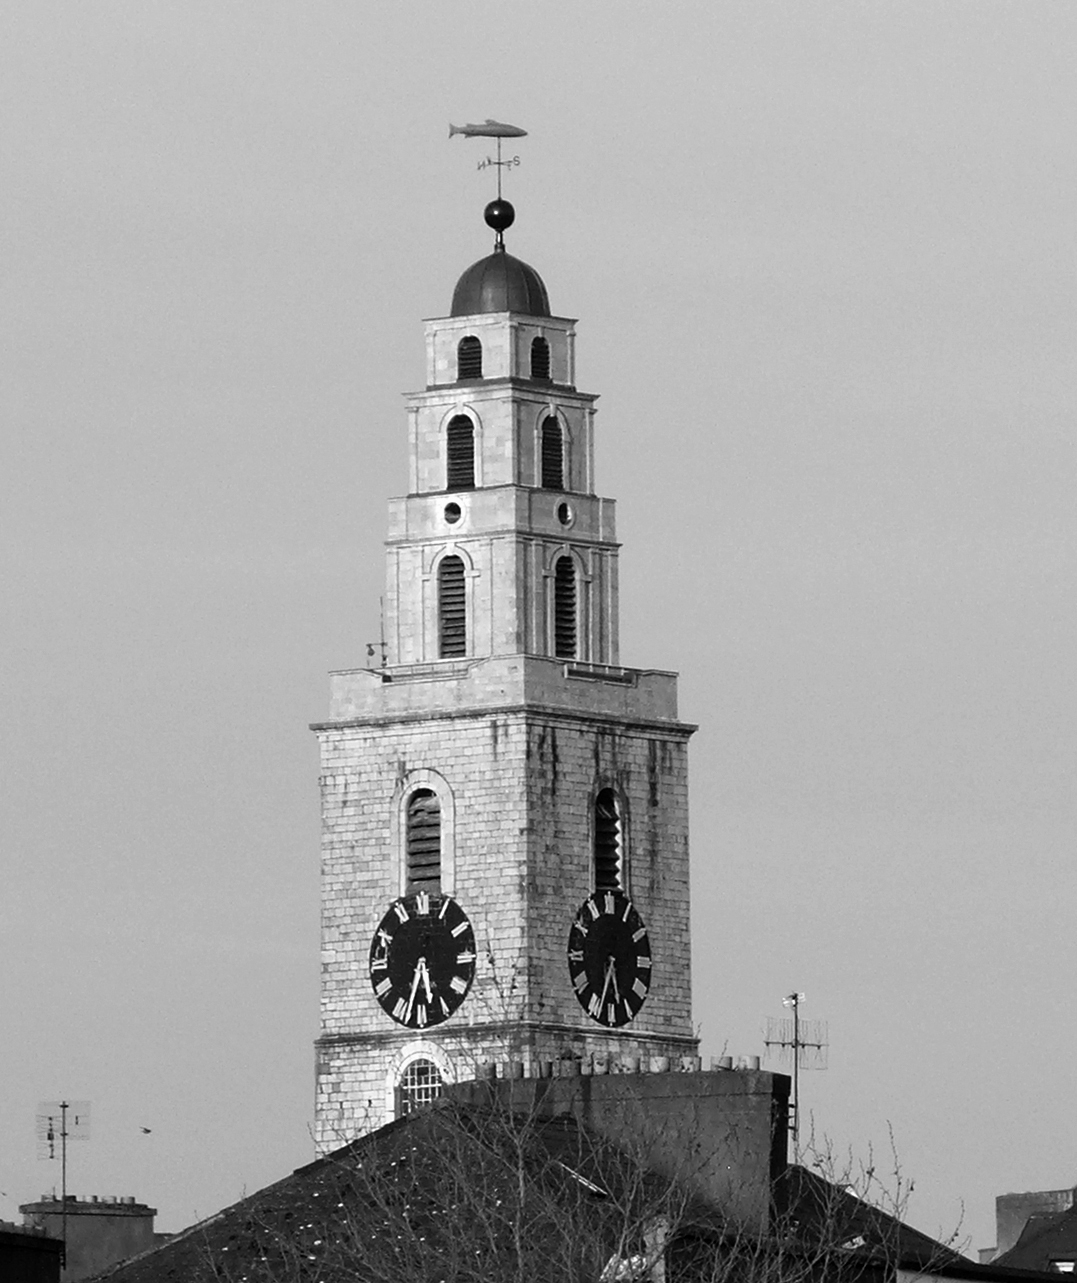
\includegraphics[height=.5\textheight]{img/Shandon_bells_cork.BW.jpg}
  \caption[
    Classical Time. The \emph{Four Faced Liar}, Shandon Bells, Cork
  ]{
    Classical Time and errors.
    % The \emph{Four Faced Liar}
    % (Shandon Bells, St. Anne's Church, Cork).
    % These four clocks
    % may famously
    % indicate slightly different times from each other.
    ``Each side of the [Shandon Bells] tower also contains a clock face.
    Installed in 1847 and affectionately known as the
    `four-faced liar', the hands on the east and west run slightly fast, especially in windy weather.
    This is probably because they are so very large
    (only Big Ben in London has larger clock faces).''
    \parencite{CorkStrolls}. Photo source: \cite{ShandonBells}.
  }
  %\vspace{3\baselineskip}
  \label{fig:ShandonBells}
\end{figure}
\end{savenotes}

\subsection{Time evolution, relativity, photons}\label{sec:trel}

The idea of a perfect analogy between
position--momentum and time--energy uncertainty relations 
might naturally lead one to ask whether position and time
(or space and time coordinates), as well as momentum and energy, can be trated on
equal footing. This is what (classically) happens within Einstein's theory of relativity.
Thus, one may further wonder:
would a theory combining quantum mechanics and
relativity be the suitable framework which would allow a rigorous and logically consistent
definition of a time observable,
possibly exposing some analogy with the position operator?

None of the proposed models comprehending both quantum theory and \emph{general} relativity
have reached general consensus,
or the remote possibility of experimental verification \parencite{QGravIntro};
but \term{quantum field theory} (QFT) is an established framework that does combine
some principles
of quantum mechanics with the \emph{special} theory of relativity.

Unfortunately, QFT does not promote time $t$ to some quantum operator $\hat{t}$;
instead, it achieves equal treatment of space and time only by
``demoting'' the \emph{position} operator to a mere classical parameter.\footnote{
  More on this in Section \ref{sec:KG}, where the Klein-Gordon equation is reformulated
  with time as an Hermitian operator in an appropriate Hilbert space
  ---based on the Page--Wootters model, which is introduced in Chapter~\ref{ch:pw}.
}
It treats time and space equally only in the sense that they are all classical,
which appears as the necessary tradeoff in order to quantize other quantities
in some mathematically tractable way. \parencite[\s I.1]{SrednickiQFT}.

It is no surprise that one of the most successful applications
of QFT, the Standard Model, describes all fundamental interactions except gravity:
while electroweak and strong interactions can be described within a field theory
which treats time and space as a ``background'' (or \emph{labels} to mark the relevant operators),
time and space are expected to be the main mathematical objects (observables),
and transform appropriately,
in a theory of gravity
which has general relativity as its classical counterpart.
Whether the definition of a quantum time operator is an useful step towards
a quantum theory of gravity is, of course, beyond the scope of the present work.

The fact that QFT ``externalizes'' time and position to the rank of classical parameters
is particularly true in quantum electrodynamics, also within the
phenomenology of quantum optics.
Thus it is impossible to define a \emph{photon} position
within standard quantum optics (see, for example, \cite{ScullyZubairy}, sec. 1.5.4 `Wave function for photons'),
and the problem of defining a quantum position observable for a photon
shows an interesting analogy with time for a quantum massive particle.
It is, in fact, a matter of active research \parencite{HawtonPhotonPosition, Hawton2019}.

While there is not a wave function for photons, the wave function for massive particles,
as seen in the Shr\"{o}dinger equation, only exists as a function of position (or momentum, etc.)
but not as a function of time,
i.e. the variable $t$ in Eq.~\eqref{eq:diracdeltaxt}
cannot be regarded as spanning the spectrum of a time operator.

Nevertheless, we have provided an explanation as to why (even without considering the Pauli objection)
relativistic field theories, as currently accepted, cannot provide a solution
to the problem of quantum time, in spite of treating time and space on equal footing,
and despite the fact that position in quantum mechanics is an observable
with its associated self-adjoint operator.

\section{Structure of the thesis}\label{sec:struct}

After explaining the motivation behind this work in Chapter \ref{ch:intro},
a review of open quantum systems and non-projective measurement theory
is outlined in Chapter~\ref{ch:decohere}, as a necessary ``toolbox''
to understand relational models and other theoretical formulations
of time as a quantum observable.

The \emph{Pauli objection} itself is detailed in Chapter \ref{ch:hist},
together with some models that have been proposed to overcome it,
with the exception of relation models, and in particular the Page--Wootters model
of ``evolution without evolution'',
which is presented in Chapter~\ref{ch:pw},
where it is also compared to some detector models.
Therein, results are compared in relation to some systems of particular interest,
and possible analogies are explored.

Further areas of study and applications are suggested in Chapter \ref{ch:outlook}.

\chapter{Quantum Measurement Theory:~a review}\label{ch:decohere}
%% With appendices moved here, this chapter is much less
%% about (reletalively recent) research and more
%% textbook-like.

This chapter is devoted to briefly recall some
foundations and modern developments of quantum measurement theory.
It's strongly based on works like
\cite{PreskillNotes, Haroche_Exploring, Nakahara, NielsenChuang, open_systems},
where they are presented in the context of
open quantum systems and quantum information theory.

\section{Bipartite systems, separable and entangled states}

Consider a \term{bipartite quantum system}
i.e. a composite system $S$
made up of two parts, $A$ and~$B$,
described by their respective Hilbert spaces
$\hilb{H}_A$ and $\hilb{H}_B$.

Notably, in \cite{Haroche_Exploring},
notation does not treat the two spaces
on perfectly equal footing,
in the sense that a basis for $\hilb{H}_A$ and a basis for $\hilb{H}_B$
are indicated as
$$
  \setof{\ket{i_A}} \text{ and } \setof{\ket{\mu_B}}\,
$$
with latin and greek indices to label base vectors in the two spaces.
We will follow such convention unless otherwise specified.

This indicates different physical roles for the two spaces,
such as the \emph{system of interest} and the surrounding \emph{environment},
or the \emph{system being measured} and the \emph{measurement apparatus}.

If the two subsystems are prepared independently and not let interact with each other,
the system is in a \term{product state} or \term{separable state}:
\begin{equation}\label{eq:separableAB}
  \ket{\psi_S} = \ket{\psi_A}\otimes\ket{\psi_A} \,\text{.}
\end{equation}

It's worth recalling that in a tensor product space $\hilb{H}_A\otimes\hilb{H}_B$
not all vectors can be expressed as a tensor product as in \eqref{eq:separableAB}.
However, the following holds:

\begin{proposition}\label{TensorBase}
The set of tensor products of base vectors of $\hilb{H}_A$ and $\hilb{H}_B$,
i.e. $$\setof{\ket{i_A} \otimes \ket{\mu_B}}_{i\mu},$$
is a basis for $\hilb{H}_A \otimes \hilb{H}_B$
\end{proposition}
Therefore, we can express any
(generally not separable) state vector of $\hilb{H}_S$
as a \emph{superposition} of separable base vectors
\begin{equation}\label{eq:bipartite_expansion}
  \ket{\psi_S} = \sum_{i, \mu}\alpha_{i\mu}\ket{i_A}\otimes\ket{\mu_B} \neq \ket{\psi_A}\otimes\ket{\psi_B},
\end{equation}
meaning that the
``total'' $\ket{\psi_A}$ and $\ket{\psi_B}$ don't necessarily exist.

Non separable states are said \term{entangled}.

Physically,
$\ket{\psi_S}$ contains information
not only about the results of measurements on $A$ and $B$ separately,
but also on correlations between these measurements.

The simplest example of entangled system is given by two two-level systems,
namely two spin-$\frac{1}{2}$ particles in a singlet state:
\[
  \ket{\psi_{\text{singlet}}} = \frac{1}{\sqrt{2}} \left(\ket{\uparrow, \downarrow} - \ket{\downarrow, \uparrow}\right).
\]

\section{Density operator}\label{app:density}

A quantum state (either pure or \term{mixed}),
is generally described by a \term{density} operator (or density matrix) $\rho$.

The general expression for a density operator $\rho$ is
$$
  \rho = \sum_{k}p_{k}\ketbra{\psi_{k}}
$$
with $p_{k}$ being non negative and $\sum_{k}p_{k} = 1$;
where $p_k$ indicates the ``classical'' probability of the system to be in state $\ket{\psi_{k}}$.

For a pure state (corresponding to ket $\ket{\psi}$) the density operator reduces to
\[
  \rho_{(\text{pure})} = \ketbra{\psi}\,\text{.}
\]

The expectation value of an observable represented by the operator $A$
is given by \parencite{BlumDensity, FanoDensity}
\begin{equation}\label{eq:expvalA_rho}
  \expval{A} = \tr(A\rho)\,.
\end{equation}

Eq. \eqref{eq:expvalA_rho} is valid for any Hermitian operator $A$. Particularly,
it is also valid if $A$ is a \emph{projector} and we will use this
e.g. in Proposition \ref{probability_rho}.

We will now look at some properties of the density operator.

We can prove the following
\begin{proposition}
  Let $A$ be an Hermitian operator
  a complete set of eigenvectors $\{\ket{m}\}$
  and
  such that
  $$
    \tr(A\rho) = 0
  $$
  \emph{for any density operator} $\rho$.
  It follows that $A = 0$.

  \begin{proof}
    We can choose
    ---to explicitly evaluate the expression of the trace---
    for each positive integer $n$,
    a particular density operator $\rho = \ketbra{n}$,
    corresponding to a (pure) eigenstate of $A$.

    With this particular choice,
    for each $n$,
    $$
      A\rho = \mel{n}{A}{n}\ketbra{n}\,.
    $$
    It then follows:
    \begin{multline}\label{eq:qmt:alldiagzero}
      0 = \tr(A\rho) = \sum_{m}\mel{m}{ ( \mel{n}{A}{n}\ketbra{n} ) }{m} = \\
          \sum_{m} \mel{n}{A}{n} \braket{m}{n} \braket{n}{m}
        = \mel{n}{A}{n} .
    \end{multline}
    With respect to the basis $\setof{\ket{n}}$ the operator $A$ is
    represented by a matrix whose elements are given by $a_{nm} = \mel{n}{A}{m}$;
    but $\setof{\ket{n}}$ is an eigenbasis, therefore we are only interested in the diagonal
    elements (the off-diagonal ones being zero).
    However, the diagonal elements are  $\mel{n}{A}{n} = 0$
    for all $n$, according to Eq.~\eqref{eq:qmt:alldiagzero}, therefore the operator itself is $A=0$.
  \end{proof}
\end{proposition}

The \emph{additivity} property follows immediately:

\begin{corollary}
If $\tr(A\rho) + \tr(B\rho) = \tr(C\rho)$ for any density operator $\rho$,
then $A + B = C$.
\end{corollary}

\section{Partial trace and open systems}
\label{sec:p_tr}

In a bipartite system, one subsystem considered alone is an
\emph{open quantum system},
while the system as a whole is still a closed systems.

Now, let's consider an observable $M_A$, acting only on subsystems $A$.
It can be expressed in $\hilb{H}_A \otimes \hilb{H}_B$ as
\[
  M_A \otimes \idop_B\, .
\]
Its expectation value is
(using the expansion in Eq.~\eqref{eq:bipartite_expansion},
and the notation of Latin indices for system $A$ and Greek ones for system $B$)
\begin{multline}\label{eq:exp_subsys}
  \expval{M_A} = \matrixel{\psi_S}{M_A\otimes\idop_B}{\psi_S} = \\[1em]
  \sum_{j,\nu}a^{*}_{j\nu}\left(\bra{j}\otimes\bra{\nu}\right)\left(M_A\otimes\idop_B\right)\sum_{i,\mu}a_{i\mu}\left(\ket{i}\otimes\ket{\mu}\right) = \\
  \sum_{j,\nu,i,\mu}a^{*}_{j\nu}a_{i\mu}\matrixel{j}{M}{i}\matrixel{\mu}{\idop}{\nu} =
  \sum_{j,\mu,i}a^{*}_{j\mu}a_{i\mu}\matrixel{j}{M}{i}
\end{multline}

The bra $\bra{\mu}$, when acting on a ket element of $\hilb{H}_{A} \ox \hilb{H}_{B}$,
can be defined
as a map from $\hilb{H}_A\otimes\hilb{H}_B$ to $\hilb{H}_A$.

A formal definition can be given in terms of how it acts upon a generic
basis ket of $\hilb{H}_A\otimes\hilb{H}_B$.

\begin{definition}\label{def:pBra}
\[
  \braket{\mu}{i\nu} = \bra{\mu}\Big(\ket{i}\otimes\ket{\nu}\Big) \eqbydef \delta_{\mu\nu}\ket{i} \text{.}
\]
\end{definition}

Intuitively, $\bra{\mu}$ is then a ``partial bra''
as it only maps the ``$\ket{\nu}$'' part of\\
``$\ket{i}\otimes\ket{\nu}$''
to a number:
\[
  \begin{array}{cccc}
    \bra{\mu}:  & \ket{i}\ox\ket{\nu}                   & \rightarrow & \delta_{\mu\nu}\ket{i}                \\
                & \rotatebox[origin=c]{270}{$\in$}      &             & \rotatebox[origin=c]{270}{$\in$}      \\
                & \hilb{H}_A\ox\hilb{H}_B               &             & \hilb{H}_A   \text{.}
  \end{array}
\]

This is consistent with the idea of
``tracing out the environment'' within an interpretation where
$\hilb{H}_B$ is the environment, and ultimately with the goal of
studying subsystem $A$ alone in spite of its entanglement with the
``environment'' (or measurement apparatus etc.) modeled by
subsystem $B$.

Conversely,
the ket $\ket{\mu}$, when acting on a bra element of $\hilb{H}_{A} \ox \hilb{H}_{B}$,
can also be defined
as a map from $\hilb{H}_A\otimes\hilb{H}_B$ to $\hilb{H}_A$.
The following definition of $\ket{\mu}$ is simply \term{dual} to Definition \ref{def:pBra}:
\begin{definition}\label{def:pKet}
  \[
    \braket{i\nu}{\mu} = \Big(\bra{i}\ox\bra{\nu}\Big)\ket{\mu} \eqbydef \delta_{\mu\nu}\bra{i} \text{.}
  \]
\end{definition}
Similar considerations apply:
\[
  \begin{array}{cccc}
    \ket{\mu}:  & \bra{i}\ox\bra{\nu}                   & \rightarrow & \delta_{\mu\nu}\bra{i}               \\
                & \rotatebox[origin=c]{270}{$\in$}      &             & \rotatebox[origin=c]{270}{$\in$}      \\
                & \hilb{H}_A\ox\hilb{H}_B               &             & \hilb{H}_A     \text{.}
  \end{array}
\]

%%

The operations defined (for basis vectors) in Definition \ref{def:pBra} and \ref{def:pKet}
are called \term{partial inner products} \parencite[\s 1.3.3]{QMT_Jacobs}.
They can be extended to all vectors of $\hilb{H}_B$ and $\hilb{H}_B\ox\hilb{H}_B$
simply by linearity.

Similarly, partial inner products with bras and kets of $\hilb{H}_A$
(and values in $\hilb{H}_B$) can be defined as well.

We are now in the position to introduce the \term{partial trace}:
\begin{definition}\label{def:pTr}
  The \term{partial trace}
  is a linear map
  that takes an operator
  $M_{AB}$ on $\hilb{H}_A \otimes \hilb{H}_B$
  to an operator on $\hilb{H}_A$ defined as
  \[
    \tr_B M_{AB} = \sum_{\mu} \matrixel{\mu}{M_{AB}}{\mu}
    \, \text{,}
  \]
  where $\setof{\ket{\mu}}$ is a basis of $\hilb{H}_B$.
\end{definition}

The first thing to note is that the \emph{partial} trace is \emph{operator-valued},
its value is not a scalar as opposed to the \emph{trace}.

Next, we can introduce the \term{reduced density operator}
of system $A$, which is obtained by \emph{tracing out the environment} B,
via the partial trace:
\begin{definition}\label{def:density_A}
  If $\rho$ is the density operator of a whole bipartite system, composed of two parts $A$ and $B$,
  the \term{reduced density operator} related to subsystem $A$ is defined as
  \[
    \rho_A = \tr_B(\rho) \, \text{.}
  \]
\end{definition}

We assume now that the total state $\rho$ is a pure state $\rho = \ketbra{\psi_S}$.

If $\setof{\ket{\mu}}$ is a basis of $\hilb{H}_B$,
for each element $\ket{\mu}$,
using the definitions \ref{def:pBra} and \ref{def:pKet}
and the expansion \eqref{eq:bipartite_expansion}, we obtain
\begin{eqsplit}\label{eq:psiPartial}
  \braket{\mu}{\psi_S} &= \sum_i \alpha_{i\mu}    \ket{i} \text{,} \\
  \braket{\psi_S}{\mu} &= \sum_j \alpha_{j\mu}^{*}\bra{j} \text{.}
\end{eqsplit}

which allows us to expand the definition of reduced density operator (Definition \ref{def:density_A})
as\footnote{
  The key point of this reasoning is showing how
  a pure state of the total system can correspond to mixed states
  in the two subsystems $A$ and $B$. Therefore it is not restrictive to assume,
  in what follows,
  that the total state $\rho = \ketbra{\psi_S}$ is pure.
}

\begin{equation}\label{eq:density_A_expand}
  \rho_A = \tr_B(\ketbra{\psi_S}{\psi_S}) =
    \sum_{\mu}\braket{\mu}{\psi_S}\braket{\psi_S}{\mu} =
    \sum_{ij\mu} \alpha_{i\mu}\alpha_{j\mu}^{*}\ketbra{i}{j} \text{.}
\end{equation}

Finally, we can see that
\begin{multline*}
  \tr(M_A \rho_A) = \sum_k \mel{k}{M_A \rho_A}{k} =
    \sum_k \mel {k} {M_A \left(\sum_{ij\mu} \alpha_{i\mu}\alpha_{j\mu}^{*}\ketbra{i}{j}\right)} {k} = \\
    \sum_{ijk\mu} \alpha_{i\mu}\alpha_{j\mu}^{*} \mel{k}{M_A}{i} \braket{j}{k} =
    \sum_{ij\mu} \alpha_{i\mu}\alpha_{j\mu}^{*} \mel{j}{M_A}{i}
    \, \text{,}
\end{multline*}
which is the same result as \eqref{eq:exp_subsys}.

This allows us to conclude that
\begin{proposition}
  For an observable $M_A$, acting solely on one subsystem, the expectation value
  for state $\rho$ can be calculated as
  \begin{equation}
    \expval{M_A} = \tr(M_A \rho_A)
  \end{equation}
  where $\rho_A$ is the reduced density operator obtained from $\rho$ by
  tracing out the environment $B$ (as per Definition \ref{def:density_A}).
\end{proposition}

It's clear from \eqref{eq:density_A_expand} that $\rho_A$ is self-adjoint,
hence it can be diagonalized:
\begin{equation}\label{eq:rho_diag}
  \rho_A = \sum_a p_a \ketbra{a}{a} \text{.}
\end{equation}

Let $\setof{\ket{k}}$ be a basis of $\hilb{H}_A$.
From \eqref{eq:density_A_expand} we can also derive that
\begin{equation}
  \tr\rho_A = \sum_k \mel{k}{\rho_A}{k} =
    \sum_{ijk\mu}\alpha_{i\mu}\alpha_{j\mu}^{*}\braket{k}{i}\braket{j}{k} =
    \sum_{k\mu}\abs{\alpha_{k\mu}}^2 = 1 \text{,}
\end{equation}
where the last equality is justified by the normalization of $\ket{\psi_S}$
in \eqref{eq:bipartite_expansion}.

The trace, i.e. the sum of matrix diagonal elements, is independent
from the chosen basis, hence $\tr\rho_A = 1$ is valid in particular
for the diagonal form \eqref{eq:rho_diag}, meaning
\[
  \sum_a p_a = 1
\]
and providing a necessary condition to interpret $p_a$ as a probability.

Eq. \eqref{eq:rho_diag}, with $p_a$ as a probability, is often
given as a \emph{definition} of the density operator.
% TODO: do the calculation?
The probability distribution ${p_a}$
is described as a ``classical'' uncertainty in the preparation of the system
(for example due to an unknown interaction with the environment).

The reverse also holds true:
\begin{proposition}
A system with uncertainties in the preparation of the \emph{state}
(``mixed'') is equivalent to one part (``$A$'') of a bipartite system
entangled with the rest (``B'') such that the total system
$A+B$ is in a pure state.
\end{proposition}

The above is called \term{purification} (see e.g. \cite[\s 2.5]{NielsenChuang}).


\section{Comparison of a coherent superposition and a mixed state}
\label{sec:mix}

Given, for simplicity, a two-level system (a qubit), and an orthonormal basis
$\setof{\ket{0}, \ket{1}}$, it may be of interest to compare a \term{coherent superposition}
of the two pure states $\ket{0}$ and $\ket{1}$, with equal probability on the outcome of
a measurement (but in a well-defined quantum state); with a statistical mixture of
states $\ket{0}$ and $\ket{1}$, again with equal probability, but 
\emph{in the determination of the quantum state}.

A natural example of such coherent superposition is (e.g. \cite[Example 2.4]{Nakahara})
\[
  \ket{\psi} = \frac{1}{\sqrt{2}}\ket{0} + \frac{1}{\sqrt{2}}\ket{1}\text{,}
\]
and the corresponding density operator is
\begin{multline}\label{eq:matrix:pure}
  \rho_{\mathrm{pure}} = \ketbra{\psi}{\psi} =
  \frac{1}{2}\qty\Big(\ket{0} + \ket{1}) \qty\Big(\bra{0} + \bra{1}) =
  \frac{1}{2}\sum_{ij=0}^1\ketbra{i}{j} \repr
  \frac{1}{2}
    \begin{pmatrix}
      1 &1  \\
      1 &1  \\
    \end{pmatrix}
  \text{.}
\end{multline}
On the other hand, for the statistical mixture, the density operator is
\begin{equation}\label{eq:matrix:mix}
  \rho_{\mathrm{mix}} = \frac{1}{2}\ketbra{0}{0} + \frac{1}{2}\ketbra{1}{1} \repr
  \frac{1}{2}
    \begin{pmatrix}
      1 &0  \\
      0 &1  \\
    \end{pmatrix}
  \text{.}
\end{equation}

By comparing the matrices in \eqref{eq:matrix:pure} and \eqref{eq:matrix:mix}
we may conclude that the off-diagonal terms in the coherent superposition case
indicate \emph{coherence}, or ``'quantum purity'';
however, density operators are self-adjoint operators
(as linear combination of projectors) and can always be expressed in
diagonal form. This also includes density operators of pure states.
In this particular case all diagonal elements are zero
except one. Indeed, for a pure state:
\[
  \rho = \ketbra{\psi}{\psi}\text{,}
\]
and recalling the assumption that $\ket{\psi}$ is normalized,
we can always build a basis $\qty{\ket{e_j}}$ including $\ket{e_{j_0}} = \ket{\psi}$
among its elements, therefore the diagonal representation is
\[
  \begin{pmatrix}
    0           &       &       &       &       &           \\
                &\ddots &       &       &       &           \\
                &       &1      &       &       &           \\
                &       &       &\ddots &       &           \\
                &       &       &       &\ddots &           \\
                &       &       &       &       &0
  \end{pmatrix}\text{.}
\]

All the above allows us to conclude what follows:
\begin{remark}
  The density matrix of a pure state is either\\
  diag(000\dots1\dots000) or non-diagonal.

  So, except the special/trivial case above, a pure state must have off-diagonal terms.
\end{remark}

It's interesting, as well, to look at ensembles (mixtures)
which are not necessarily made up of orthonormal pure states.
In fact, an ensemble of orthonormal states has ``nothing special'',
and different ensembles may lead to the same density operator.
The diagonalized density matrix just shows the ``orthonormal''
ensemble which, again, has no special physical meaning.

For example, let's consider this orthogonal ensemble (diagonal density matrix):
\[
  \rho_1 = \frac{3}{4}\ketbra{0}{0} + \frac{1}{4}\ketbra{1}{1}
\]
and
\[
  \rho_2 = \frac{1}{2}\ketbra{a}{a} + \frac{1}{2}\ketbra{b}{b}\text{.}
\]
with
\begin{align*}
  \ket{a} &= \frac{4}{4}\ket{0} + \frac{1}{4}\ket{1} \\
  \ket{b} &= \frac{4}{4}\ket{0} - \frac{1}{4}\ket{1}
\end{align*}
It's easy to prove that $\rho_1 = \rho_2$. This is just a particular
case of a theorem.
\begin{theorem}{(Unitary freedom in the ensemble for density matrices).}
  The ensembles
  $\setof{p_i, \ket{\psi_i}}$ and $\setof{q_{j}, \ket{\phi_j}}$
  generate the same density operator
  $$\rho = \sum_i p_i \ketbra{\psi_i} = \sum_j q_j \ketbra{\phi_j}$$
  if and only if there exists
  a unitary matrix\footnote{
    The transformation represented by the unitary matrix $\setof{u_{ij}}$
    does not preserve the orthogonality of the vectors sets,
    which seems to contradict a fundamental property of unitary
    transformations: however, it should be noted that the coefficients
    $u_{ij}$ do not act on components of each state vector; in other
    words, $\setof{u_{ij}}$ represent a transformation acting
    on ``vectors of vectors'' and therefore is not really a unitary
    transformation in a Hilbert space.
  }
  $\setof{u_{ij}}$ such that
  \[
    \tilde{\ket{\psi_i}} = \sum_j u_{ij}\tilde{\ket{\phi_j}}
  \]
  where $\tilde{\ket{\psi_i}}$ and $\tilde{\ket{\phi_j}}$
  are the (not normalized) vectors defined as
  \[
    \tilde{\ket{\psi_i}} = p_{i}\ket{\psi_i}
    \text{ and }\,
    \tilde{\ket{\phi_j}} = q_{j}\ket{\phi_j}
  \]
\end{theorem}
See \cite[Theorem 2.6 and introductory example]{NielsenChuang}
for a more detailed description and a proof of the theorem.

%\section{Quantum and the Environment: from Quantum to Classical}
\label{sec:q2c}

In sec. \ref{sec:mix} we have considered a simple orthonormal basis
and built a statistical mixture of their vectors. We have shown
that the same density operator can be generated by other ensembles,
not necessarily orthogonal. Nonetheless, the orthonormal ensemble,
corresponding to a diagonal representation of $\rho$, \emph{is}
special, only in the sense that an orthonormal, complete set of
vectors can be seen as the eigenbasis for some observable,
and such representation is particularly expressive if the
interaction with the environment we are considering
(or the entanglement with the other part of a bi-partite system, in other terms)
is a \emph{measurement}.

A measurement turns
the (sub-)system $S$ from a coherent superposition into a
maximally mixed state like in the examples
\eqref{eq:matrix:pure} and \eqref{eq:matrix:mix}.
A quantum superposition into a classical probability
distribution of possible eigenstates.
Following this route, the Born rule, a fundamental concept in the
Copenhagen interpretation of quantum mechanics, can be
\emph{derived} instead of postulated
\parencite{Zurek_Einselect}.
Historically,
the effort in overcoming the \term{wavefunction collapse},
treating the measurement apparatus as a quantum,
and not a classical system,
was pioneered by J. von Neumann \parencite{VonNeumann}.

As a self-adjoint operator, $\rho_S$ after the interaction
can always be diagonalized, so we can conclude that any
interaction with the environment is the measurement of some
observable $A$, at least in the mathematical sense: $A$ may or
may not be of any notable physical significance.

A key concept in \cite{Zurek_Einselect} is the
\term{environment-induced superselection} or \term{einselection},
i.e. the idea that particular \term{pointer states} are not
perturbed by the \term{environmental monitoring}.
Because of their stability, they can be regarded as
\term{memory states}.

Coherent superpositions of pointer states are not pointer states
themelves, and such \emph{coherence} is destroyed in the process. 
Contrary,
or complementary to previous studies, which focused on the effect of
the environment on the system, Zurek's work
\parencite{Zurek_Einselect}
focuses on
accessibility of information spread throughout the environment,
noting that observers monitor systems indirectly, by intercepting
small fractions of their environments:
\begin{quote}
\emph{Relaxation and noise are caused by the environment perturbing
the system}, while \emph{decoherence and einselection
are caused by the system perturbing the environment}.
\end{quote}

\section{Quantum operations}

Decoherence,
or more generally the interaction of a system with the environment,
can be seen as a process of information loss for the system
\parencite[Ch. 9]{Nakahara} or information storage
\parencite{Zurek_Einselect}, if the system under consideration
is \emph{the observer}.

A \term{quantum operation} \parencite[Ch. 9]{Nakahara} is the generalization
of unitary evolution to include open systems as well as closed ones.

The evolution of the density operator for a closed system is given by the map
\[
    \rho_{S} \rightarrow U(t)\rho_{S}U^{\dagger}(t) \, \text{.}
\] 
We are looking to describe a general change
$\rho \rightarrow \mathcal{E}(\rho_{S})$ that may also include
changes due to measurement (or noise).

(continue now w/ Preskill, as Nakahara emphasizes noise over measurement, look for Krauss op.)

POVM -- Krauss.

\section{TODO}

The environment is watching, from ``Exploring the quantum''
\parencite[Ch. 4]{Haroche_Exploring}. Start with subsect. 2.4.1.

ULTIMATELY GOTO PRESKILL NOTES (Haroche "inspired by")

2.5.4 The quantum–classical boundary
Decoherence models versus Copenhagen interpretation.

Environment-Induced Decoherence and the Transition from Quantum to Classical,
\cite{Zurek_Fundamentals}.

Partial trace, which is not a number, check wikipedia $\rightarrow$ consistent histories.
J. P. Paz W. H. Zurek

Von Neumann and Shanon entropy.

MIKIO NAKAHARA: QUANTUM COMPUTING: AN OVERVIEW

See also \cite{Schlosshauer_Decoherence}.

Vedral, Brukner (Oreshkov\dots)
Necessary and sufficient condition for non-zero quantum discord
\url{https://arxiv.org/pdf/1004.0190.pdf},
cites another paper by Zurek \url{https://arxiv.org/pdf/quant-ph/0105072.pdf}.

\section{Standard measurement and generalizations}

The evolution of the density operator for a closed system is given by the map
\[
    \rho_{S} \rightarrow \mathcal{E}(\rho_{S}) = U(t)\rho_{S}U^{\dagger}(t) \, \text{.}
\] 
We are looking to describe a general more change
$\rho \rightarrow \mathcal{E}(\rho_{S})$ that may also include
changes due to measurement (or noise).

Furthermore, we are looking to describe a generalization
of projective measurement~\parencite{VonNeumann}:
when a projective, Von-Neumann
measurement is performed on a multipartite system,
it does not necessarily correspond to a projective measurement
on each subsystem~\parencite[Ch. 3]{PreskillNotes}.

\subsection{Review on projectors}

We shall assume, unless otherwise stated, that all vectors are
normalized to unity.

Consider an observable represented by a self-adjoint operator $A$
with a 
\emph{discrete, non degenerate spectrum}.
Let $a_i$ by an eigenvalue of $A$, and $\ket{i}$ its corresponding eigenvector.
The probability of a measurement
outcome $a_i$,
on a system in the pure state $\ket{\psi}$
is given by
$$
\pi_{i} = \norm{\braket{i}{\psi}}^2
        = \bra{\psi}\ket{i}\bra{i}\ket{\psi}
        = \mel{\psi}{P_{i}}{\psi}
$$
where $P_{i} = \ketbra{i}$ appears as the \term{projector} on the
one-dimensional ei\-gen\-space related to eigenvalue  $a_i$.

If $a_i$ is degenerate, $j = 1, \dots, J$ its degeneracy index, and $\ket{ij}$ the corresponding eigenvectors,
such probability shall sum over it:
$$
\pi_{i} = \sum_{j=1}^{J}\norm{\braket{ij}{\psi}}^2
        = \sum_{j=1}^{J}\bra{\psi}\ket{ij}\bra{ij}\ket{\psi}
        = \mel{\psi}{P_{i}}{\psi}
$$
where $P_{i} = \sum_{j=1}^{J}\ketbra{ij}$
still is the projector on the
($J$-dimensional) eigenspace of $a_i$.

Generally, the probability that the outcome of a measuremen falls in
the set of eigenvalues $\sigma = \{a_{1}, \dots, a_{S}\}$ is
\begin{equation}\label{eq:pi_sigma}
\pi_{\sigma}  = \sum_{i=1}^{S}\sum_{j=1}^{J_{i}}\norm{\braket{ij}{\psi}}^2
              = \sum_{i=1}^{S}\sum_{j=1}^{J_{i}}\bra{\psi}\ket{ij}\bra{ij}\ket{\psi}
              = \mel{\psi}{P_{\sigma}}{\psi}
              ,
\end{equation}
where $P_{\sigma} = \sum_{i=1}^{S}\sum_{j=1}^{J_{i}}\ketbra{ij}$
is once again a projector --- on the ``generalized eigenspace'' spanned by all
eigenvectors $\{\ket{ij}\}$ above.

Looking back at \eqref{eq:expvalA_rho},
it is valid for \emph{any} hermitean operator,
therefore it's also valid for projectors.

Hence, can replace $A$ with the projector $P_{\sigma}$,
associated to the set of eigenvalues $\sigma$
according to \eqref{eq:pi_sigma} and \eqref{eq:P_sigma_spectral}.

This is of particular interest
because its mean value equates the probability that the outcome of a measurement
falls in a given subset of the spectrum of a given observable.
So we can derive:

\begin{proposition}\label{probability_rho}
  The probability $\pi_{\sigma}$
  that the outcome of a measurement of the observable $A$
  on the system described by the state operator $\rho$
  falls in the set $\sigma$
  is given by:
  \begin{equation}\label{eq:probability_rho}
    \pi_{\sigma} = \expval{P_{\sigma}} = \tr(P_{\sigma}\rho)
  \end{equation}
  with $P_{\sigma}$ defined as in \eqref{eq:pi_sigma}
  or, more generally, in \eqref{eq:P_sigma_spectral}.
\end{proposition}

%%%%%%%%%%%%%%%%%%%%%%%%%%%%%%%%%%%%%%%%%%%%%%%%%%%%%





\subsection[Measure]{Measure\footnote{Not to be confused with \emph{measurement}.}}

\begin{remark}\label{measure_properties}
  Being $\pi_{\sigma}$ the \emph{probability} of the outcome of a measurement to
  fall in a given set $\sigma$, it has to be:
  \begin{enumerate}
    \item \label{measure_properties:first} $0$ on the empty set
    \item non negative
    \item \label{measure_properties:last} \term{additive} on disjoint sets
    \item equal to $1$ if $\sigma$ includes the whole spectrum of $A$.
  \end{enumerate}
\end{remark}

\begin{remark}
  Properties \ref{measure_properties:first}\dots\ref{measure_properties:last}
  are the defining properties of a \term{measure} \parencite{EncMath_Measure}.
\end{remark}

The probability $\pi_{\sigma}$ in \eqref{eq:pi_sigma} is linear with respect to the projector
$P_{\sigma}$ hence it's not difficult to derive that the same properties in
\autoref{measure_properties} applies to $P_{\sigma}$, \emph{in the operator sense}.
In fact, the map $\sigma \subseteq \mathbb{R} \rightarrow P_{\sigma}$
implicitly defined in~\eqref{eq:pi_sigma} is a \term{projector-valued measure}.

The result is generalized,
in such a way to include both discrete and continous spectra,
by the following \parencite{VonNeumann, Ballentine}
\begin{theorem}[spectral resolution]
  If $A$ is a self-adjoint operator,
  there is a unique projector-valued measure $E$
  defined on the Borel sets of $\mathbb{R}$
  such that
  \footnote{
    In \eqref{eq:spectral}, $a$ is a real number (not a set),
    but it's intended $E$ to be evaluated
    on the~\emph{interval}~from $-\infty$ to $a$.
  }
  \begin{equation}\label{eq:spectral}
    A=\int_{-\infty}^{\infty}a\, dE(a)
  \end{equation}
  and satisfying:
  \begin{align*}
    E(\mathbb{R})       & =\mathbf{1},\\
    E(B_{1}\cap B_{2}) & =E(B_{1})E(B_{2})\,.
  \end{align*}
\end{theorem}

In terms of this theorem, the projector in \eqref{eq:pi_sigma} is
\begin{equation}\label{eq:P_sigma_spectral}
  P_{\sigma} = E(\sigma) = \int_{a\in\sigma}dE(a)
\end{equation}
and $dE(a)$ is
---informally speaking---
infinitesimal if $a$ belongs to the continous spectrum,
finite if $a$ is a discrete eigenvalue
and zero otherwise.


\subsection{Projective measurement (Von Neumann)}

Let's consider a \term{complete}, \term{orthogonal} set of $N$ projectors
$P_0 \dots P_{N-1}$ on the Hilbert space $\hilb{H}_A$
of the system being measured;
by definition they have the properties:
\begin{align}
  \sum_n P_n  &= \idop \\
  P_i P_j     &= \delta_{ij}P_i \, \text{.}
\end{align}

On $\hilb{H}_B$ instead, describing the measurement device, let's consider
the fiducial\footnote{
  In the sense that it's assumed
  that we can arbitrarily ``reset'' (prepare) the device,
  for example at state $\ket{0}$,
  and in general
  we will find the device at one of the states
  $\ket{0}\dots\ket{N-1}$
  when we observe it (\term{pointer states}).
  Therefore, what follows \emph{is not} a derivation of the Born's rule,
  which is still a necessary postulate of quantum mechanics
  (only \cite{Zurek_Decoherence, Zurek_Einselect, Zurek_Fundamentals} push
  this point of view further). In other words, the Born rule for the system
  will be ``proved''
  only on the assumption that it is valid for the measurement apparatus already.
}
basis:
\[
  \setof{\ket{0} \dots \ket{N-1}} \text{.}
\]

The coupling between the system and the apparatus
can be modelled by
a unitary operator
transforming the state of system and apparatus before and after the measurement.

As we will show, the following is a possible example:
\begin{equation}\label{eq:unitary_measurement}
  U = \sum_{a, b = 0}^{N-1} P_a \ox \ketbra{b+a}{b} \text{,}
\end{equation}
where the sum $b+a$ is \emph{modulo N}.

\begin{eqsplit}\label{eq:explicit_measurement_evolution}
  U:  &\ket{\Psi}           =\ket{\psi} \ox \ket{0} \rightarrow \\
      &\ket{\Psi^{\prime}}  =\sum_{a, b} P_A \ox \ketbra{b+a}{b} \qty(\ket{\psi} \ox \ket{0})
\end{eqsplit}
Indeed, in the \ref{eq:explicit_measurement_evolution} only terms with $b=0$ survive.
Therefore
\begin{eqsplit}\label{eq:measurement_entangled}
  \ket{\Psi^{\prime}} &= \sum_a \qty\Big(P_a\ox\ketbra{a}{0}) \qty\Big(\ket{\psi}\ox\ket{0}) \\
                      &= \sum_a P_a \ket{\psi} \ox \ket{a}
\end{eqsplit}

If we measure the pointer in the fiducial basis
(Hilbert space of the measurement apparatus),
the probability of an outcome $a$ is
\begin{multline}\label{eq:measurement_probability}
  \Pr(a) = \expval{\qty\Big(\idop\ox\ketbra{a})}{\Psi^{\prime}} = \\
    \sum_{b,c}
      \qty(\bra{\psi}P_{b}\ox\bra{b})
      \qty\Big(\idop\ox\ketbra{a})
      \qty(P_{c}\ket{\psi}\ox\ket{c}) = \\
    \sum_{b,c}\qty\Big(\expval{P_bP_c}{\psi} \braket{b}{a} \braket{a}{c}) =
    \expval{P_a}{\psi}
\end{multline}
which shows that the Born's rule has been ``transferred'', from the system being
measured, to the measurement device and therefore the
\eqref{eq:unitary_measurement} is a correct description of measurement.

The \eqref{eq:measurement_entangled} clearly shows that the system
and the measurement device are completely correlated (entangled).
If the measurement apparatus is observed in state $\ket{a}$
---with probability $\Pr(a)$ as stated in \eqref{eq:measurement_probability}---
then the system being measured is in state $E_{a}\ket{\psi}$
or, in normalized form:
\begin{equation}\label{eq:normalized_collapse}
  \ket{\psi^\prime_a} \eqbydef \frac{P_{a}\ket{\psi}}{\norm{P_{a}\ket{\psi}}}
    = \frac{P_{a}\ket{\psi}}{\sqrt{\expval{P_a}{\psi}}} \,\text{.}
\end{equation}

This is the \term{wave function collapse} described in terms of a unitary
transformation \eqref{eq:unitary_measurement}
acting on the system + detector compound system and describing
the measurement process
(instead of just being postulated as part of the Born's rule).
See \cite[sec.2.5.4, \emph{Decoherence models versus Copenhagen interpretation}]{Haroche_Exploring},
for a closer conceptual examination.

Indeed,
$\ket{\psi}$
is transformed
into its projection $\ket{\psi^\prime_a}$
onto the eigenspace
corresponding to the eigenvalue $a$ of the observable of interest.

The above \emph{is not} a derivation of the Born (probability) rule altogether,
as it still needs to be postulated for the measurement apparatus.

Finally, if the measurement apparatus is not observed,
therefore an outcome $a$ is not known,
the system after measurement is in a statistical mixture
of ``all possible collapses'' weighted on the probability $\Pr(a)$.
By using both \eqref{eq:measurement_probability} and \eqref{eq:normalized_collapse},
and the definition of the density operator for the initial pure state
$\rho = \ketbra{\psi}$:
\[
  \rho^{\prime} = \sum_a \Pr(a) \ketbra{\psi^{\prime}_a} = \sum_a P_a \ketbra{\psi} P_a
    = \sum_a P_a \rho P_a \,\text{.}
\]
So, the initial pure state $\rho$ is transformed by the measurement process into a mixed one.
It is said that the initial, coherent superposition of eigenstates represented by $\rho = \ketbra{\psi}$
\term{decoheres} towards the maximal statistical mixture $\rho^{\prime}$
(as seen in Section \ref{sec:mix}).

It can be proven that the transformation
\begin{equation}\label{eq:irreversible_measurement}
  \rho \rightarrow \sum_a P_a \rho P_a
\end{equation}
is also valid in the more general case of $\rho$ being a mixed state before the measurement
---in this case, it's transformed into another mixed state,
but still described by the \eqref{eq:irreversible_measurement}.
A generalization to observables with a continuous spectrum is also possible
(see e.g. \cite[Section 3.1.1]{PreskillNotes} for more details).


\subsection{Generalized measurement (POVM)}
\label{subsec:POVM}

Let's start considering, for simplicity, a 2-level system,
the corresponding 2-level pointer space,
and the unitary transformation describing the measurement process:
\begin{multline}\label{eq:qubit_ortho_measurement}
  U:
    \ket{\psi}_A \ox \ket{0}_B
    {\color{gray}= \qty\big{\alpha\ket{0}_A + \beta\ket{1}_A} \ox \ket{0}_B}
  \rightarrow \\
    {\color{gray}\alpha\ket{0}_A \ox \ket{0}_B + \beta\ket{1}_A  \ox \ket{1}_B =}
    \:
    E_0\ket{\psi}_A \ox \ket{0}_B + E_1\ket{\psi}_A \ox \ket{1}_B
\end{multline}
with subscripts $A$ and $B$ designating the system of interest and
the measurement apparatus (pointer space) respectively.

When we observe the pointer, let's assume we're not
able to ``measure'' it with respect to the fiducial basis
$\setof{\ket{0}, \ket{1}}$,
but with respect to another basis, say,
\begin{equation}\label{eq:pmbasis}
\setof{\ket{\pm} = \frac{1}{\sqrt{2}} \qty\Big(\ket{0}_B \pm \ket{1}_B)} \,\text{.}
\end{equation}

We can rewrite \eqref{eq:qubit_ortho_measurement} as
\begin{multline}\label{eq:qubit_gen_measurement}
  U: \ket{\psi}_A \ox \ket{0}_B                   \rightarrow \\
  \frac{1}{\sqrt{2}} \qty\Big(
    \alpha\ket{0}_A \ox \qty(\ket{+}+\ket{-}) +
    \beta \ket{1}_A \ox \qty(\ket{+}-\ket{-})
  )                                               =           \\
  \frac{1}{\sqrt{2}} \qty\Big(
    \qty(\alpha\ket{0}_A + \beta\ket{1}_A) \ox \ket{+} +
    \qty(\alpha\ket{0}_A - \beta\ket{1}_A) \ox \ket{-}
  )                                               \eqbydef      \\
  M_+\ket{\psi}_A \ox \ket{+} + M_-\ket{\psi}_A \ox \ket{-}
  \,\text{,}
\end{multline}
where we have defined:
\begin{align*}
  &
  M_+ \repr \frac{1}{\sqrt{2}}\mqty(\imat{2})
  &
  M_- \repr \frac{1}{\sqrt{2}}\mqty(1& 0\\0& -1)
\end{align*}
with respect to the basis $\setof{\ket{0}_A, \ket{1}_A}$.

After measurement, system $A$ is ``prepared''
(up to a normalization factor)
in one of the states $M_{\pm}\ket{\psi}$,
that are not necessarily orthogonal.

Moreover, $M_+$ and $M_-$ are not generally idempotent,
therefore if we repeat the measurement we don't generally
obtain the same result (and don't leave the system $A$ in the same state).
This is a fundamental difference with projective measurement.

Besides this particular example, $M_+$ and $M_-$ are not even necessarily
self-adjoint, and we can see that, while $M$ generalise the projector $P$
in terms of ``collapsing'' (or ``preparing'') the system under measurement,
in some sense a better generalization is in fact $M^{\dagger}M$\footnote{
  Such distinction is inessential for a projector $P$,
  as $P^{\dagger}P = P^2 = P$.
}, particularly in the sense of \term{decomposition of the identity}:
$\sum_a M_a^{\dagger}M_a = \idop$ \parencite[sec.3.1]{PreskillNotes}.

The example of $\ket{\pm}$ is a particularly ``unsharp'' measurement,
or a particularly ``overlapping'' decomposition of the identity,
because
$$M_+^{\dagger}M_+ = M_-^{\dagger}M_- = \frac{1}{2}\idop\text{.}$$

Generalizing to $N$-dimensional Hilbert spaces, we can replace
$\setof{\ket{\pm}}$ basis with
\[
  \setof{\ket{a}, a = 0\ldots N-1}
\]
and \eqref{eq:qubit_gen_measurement} with
\begin{equation}\label{eq:gen_measurement}
  U: \ket{\psi}_A \ox \ket{0}_B \rightarrow \sum_a M_a\ket{\psi}_A \ox \ket{a}_B
  \,\text{.}
\end{equation}

So, let's define
\[
  E_a = M^{\dagger}M \,\text{.}
\]

\citereset
All the following holds \parencite[sec.3.1]{PreskillNotes}:
\begin{enumerate}
  \item 
    Hermiticity: \[E_a = E_a^{\dagger}\,\text{;}\]
  \item
    \term{Positivity}: \[\expval{E_a}{\psi} \geq 0\,\text{;}\]  
  \item\label{listitem:POVM}
    Decomposition of the identity (\term{completeness}):
    \begin{equation}\label{eq:POVM}
      \sum_a E_a = \sum_a M_a^{\dagger}M_a = \idop \,\text{;}
    \end{equation}
  \item
    Probability of outcome $a$ of a measurement:
    \[\Pr(a) = \norm{M_a\ket{\psi}}^2 = \expval{E_a}{\psi}\,\text{;}\]
  \item
    Probability of obtaining $b$ in a second measurement:
    \[\Pr(b|a) = \frac{\norm{M_bM_a\ket{\psi}}^2}{\norm{M_a\ket{\psi}}^2}\]
    (would be $\delta_{ab}$ if orthogonal);
  \item
    Probability of outcome, density operator form:
    \[\Pr(a) = \tr(\rho E_a)\,\text{,}\]
    also valid for mixed states.
\end{enumerate}

This partition of the identity by positive operators
as expressed in \eqref{eq:POVM} is called
\term{positive operator-valued measure}, or \term{POVM}.
It generalises the \term{projector-valued measure} (PVM)
found in Von Neumann's theory.

For the sake if simplicity, we're referring to the finite dimensional case,
but the above can be extended to infinite dimensions and continuous spectra,
where the decomposition of the identity can be expressed as
$\int_{-\infty}^{\infty} dx M^{\dagger}(x)M(x) = \idop $.
A more abstract and general definition of POVM is as
follows:\footnote{
  See e.g. \cite{BeneduciPhD, Berberian} --- the level of generalization may vary.
}
\begin{definition}
  Given a (Borel) $\sigma$-algebra $\mathcal{B}(\mathbb{R})$ of subsets of $\mathbb{R}$,
  and the space $\mathcal{F}(\hilb{H})$ of positive, self-adjoint operators on a Hilbert space,
  a \term{positive operator-valued measure} (\term{POVM})
  is a map $E: \mathcal{B}(\mathbb{R}) \rightarrow \mathcal{F}(\hilb{H})$
  such that
  \begin{itemize}
    \item $E(\mathbb{R}) = \idop$ (completeness)
    \item $E\qty(\bigcup\limits_{n} \Delta_n) = \sum\limits_{n} E\qty(\Delta_n)$ (additivity) 
  \end{itemize}
  where $\setof{\Delta_n}$ is a countable family of disjoint sets in
  $\mathcal{B}(\mathbb{R})$.
\end{definition}

\citereset
It's worth noting that,
given a POVM $E$, operators $M$
suitable for \eqref{eq:POVM} and \eqref{eq:gen_measurement}
and following generalization
can always be found \parencite[sec.3.1]{PreskillNotes},
but not uniquely, in the sense that
$UM$ are also valid
for any unitary operator $U$.

Therefore, this formulation leaves the state after a measurement
with outcome $a$
\[
  \frac{M_a\ket{\psi}}{\norm{M_a\ket{\psi}}^2}
  \leftrightarrow
  \frac{UM_a\ket{\psi}}{\norm{M_a\ket{\psi}}^2}
\]
in fact \emph{undetermined}.

\section{Quantum channels and Kraus operators}

We have seen so far that:
\begin{enumerate}
\item
  Given a bipartite system
  described by the Hilbert space
  $\hilb{H}_A\ox\hilb{H}_B$,
  the susbsystem in $\hilb{H}_A$
  is not necessarily in a pure state itself; it
  may have the properties of a mixed state.
  (Section \ref{sec:p_tr}).
\item
  An orthogonal measurement of the bipartite system can realise a
  (non-orthogonal) POVM on $\hilb{H}_A$ alone (Subsection \ref{subsec:POVM}).
\end{enumerate}

It is therefore of interest to study
the evolution (as a density matrix in $\hilb{H}_A$) of subsystem $A$ alone,
while the bipartite system as a whole evolve unitarily.
The system $A$ alone
is initially described by the density operator $\rho=\ketbra{\psi}$.
By tracing out
$B$
(in the sense of Section \ref{sec:p_tr}),
there has:
\begin{equation}\label{eq:channel}
  \rho \rightarrow \superop{E}(\rho) \eqbydef \sum_a M_a \rho M_a^{\dagger}
\end{equation}
which generalises the unitary evolution $\rho \rightarrow U \rho U^{\dagger}$.

The linear map, or ``superoperator'',\footnote{
  A \emph{superoperator} is a linear map that associates an operator
  in a Hilbert space to another operator (instead of a vector to another vector).
}
$\superop{E}$
is called \term{quantum channel}.\footnote{
  Another name for it is
  \term{trace-preserving completely positive map},
  or \term{TPCP map} for short. \parencite[sec.3.2]{PreskillNotes}
}
The word ``channel'' is drawn from communication theory,
as the state $\rho$ can be interpreted as being \emph{transmitted}
through
a communication link from a sender to another party
who receives it modified into the state $\superop{E}(\rho)$.

A quantum channel $\superop{E}$
\begin{enumerate}
  \item is linear:
    $\superop{E}(\alpha\rho_1+\beta\rho_2) = \alpha\superop{E}(\rho_1) + \beta\superop{E}(\rho_2)$;
  \item preserves hermiticity:
    $\rho = \rho^{\dagger} \implies \superop{E}(\rho) = \superop{E}(\rho)^{\dagger}$;
  \item preserves positivity:
    $\rho = \rho^{\dagger} \geq 0 \implies \superop{E}(\rho) \geq 0$;
  \item preserves trace:
    $\tr(\superop{E}(\rho)) = \tr(\rho)$.
  \item is \term{completely positive}.\footnote{\citereset
      \cite[sec. 3.2.6]{PreskillNotes}; \cite[sec. 8.2.4]{NielsenChuang}.
    } If $\hilb{H}_R$
    is another Hilbert space of arbitrary dimension,
    then $\superop{E} \ox \idop_{R}$ is also positive
    in $\hilb{H}_A \ox \hilb{H}_R$.
\end{enumerate}

Expressing $\superop{E}$ in terms of operators $M_a$
satisfying the partition of the identity \eqref{eq:qmt:postulate:completeness}
is called
\term{operator-sum representation} of the quantum channel.

The operators $\setof{M_a}$ are called the \term{Kraus operators}
of the channel.

Similarly to POVM $\setof{E_a}$, given a particular channel $\superop{E}$,
the set $\setof{M_a}$ is not uniquely determined, but
generally exists.

A fundamental comparison with unitary evolution is that
quantum channels can be \emph{composed} too, but \emph{an inverse
does not generally exist}.
The fact that the existance of an inverse is not guaranteed corresponds,
mathematically, to the concept of \term{semigroup}
and, physically, to the \emph{irreversibility} of the process
of entanglement of subsystem $A$ with the environment. In other words,
there is no quantum channel that will bring back an entangled,
mixed state back to its initial pure state;
but a generalized evolution from time $t_0$ to time $t_1$,
described by $\superop{E}_1$,
and another from $t_1$ to $t_2$ described by $\superop{E}_2$
can be combined to describe the evolution from $t_0$ to $t_2$:
\[
  \rho \rightarrow \qty(\superop{E}_1 \circ \superop{E}_2) (\rho) =
  \sum_{\mu,a} N_{\mu} M_a \rho M_a^{\dagger} N_{\mu}^{\dagger}
  \,\text{.}
\]
If we demand that $\superop{E}_1 \circ \superop{E}_2$
is the identity (or ``superidentity'', should we say),
in other words that $\superop{E}_2$
is the \term{inverse} of $\superop{E}_1$,
we can prove that the channel must be unitary i.e.
$\superop{E}_1(\rho) = U \rho U^{\dagger}$
for some unitary evolution operator $U$.
This excludes decoherence,
or entanglement with environment from an initial pure state,
from being reversible.
See \cite[sec.3.2]{PreskillNotes} for a detailed proof,
and general properties of quantum channels.


\chapter{Pauli's objection and historical developments}\label{ch:hist}
\section{Pauli's objection}\label{proof}

The existence of a time operator with the properties required in Section \ref{sec:T--H}
is hindered by a fundamental objection
which was raised by W.~Pauli for the first time
in his \term{General Principles of Quantum Mechanics}, dated 1933,
where he argued that the existence of a self-adjoint operator,
conjugate to the Hamiltonian,
would lead to absurd consequences on the energy spectrum.
He did not provide a formal proof of his argument,
and only relegated his observation into a footnote
of his work
\parencite{PauliFootnote}; but that was sufficient to
lead most physicists to insist that ``time is just a parameter''
in quantum mechanics
since then.

Here we aim at providing
a more technical proof of Pauli's ``theorem'',
based on some relatively recent work by
E. Galapon \parencite{Galapon2002},
while expanding some details further.
A preliminary Lemma on commutator algebra follows.

\begin{lemma}\label{CommProp}
  If the commutator $[T, H]$ commutes with $T$ i.e.
  $$[T, H]T~=~T[T, H]\,,$$ then the following holds:
  \begin{equation}\label{eq:tkh}
  [T^k, H] = kT^{k-1}[T, H]\,.
  \end{equation}
  \end{lemma}
  This is particularly true when $[T, H]$ is a \emph{number} as in \eqref{THcommutator} where
  $T$ and $H$ are the time and energy operator respectively.
  \begin{proof}
  First of all, the \eqref{eq:tkh} is trivially valid for $k = 1$.

  For an arbitrary positive integer $k > 1$ there has:
  \begin{dmath}\label{tkhrecur}
  [T^k, H] = T^{k-1}TH - HT^{k-1}T = T^{k-1}TH - T^{k-1}HT + T^{k-1}HT - HT^{k-1}T \\
      = T^{k-1}[T, H] + [T^{k-1}, H]T
  \end{dmath}
  Now, iterating the result in \eqref{tkhrecur},
  \begin{dmath}\label{tkhrecurplus}
  [T^k, H] = T^{k-1}[T, H] + [T^{k-1}, H]T
  = T^{k-1}[T, H] + (T^{k-2}[T, H] + [T^{k-2}, H]T)T
  = T^{k-1}[T, H] +  T^{k-1}[T, H] + [T^{k-2}, H]T^2
  = 2T^{k-1}[T, H] + [T^{k-2}, H]T^2
  = \hdots
  = nT^{k-1}[T, H] + [T^{k-n}, H]T^n = \hdots
  \end{dmath}
  where the commutativity hypothesis $[T, H]T = T[T, H]$ has been used to obtain
  $$T^{k-2}[T, H]T = T^{k-1}[T, H]\text{.}$$

  Now, \eqref{tkhrecurplus} can be continued until it reaches $n=k$ when the term
  $[T^{k-n}, H]T^n$ vanishes and a result of $kT^{k-1}[T, H]$ follows.
  \end{proof}
\normalsize

Let us now come to the Pauli argument; and
assume that there exists a self-adjoint time operator, $T$, canonically conjugate
to the Hamiltonian $H$, i.e.

\begin{equation}
\label{THcommutator}
[T, H] = i\hbar
\end{equation}
Since T is self-adjoint, then for all
$\beta\in\mathbb{R}$, $U_{\beta} = \exp(- i \beta T / \hbar)$
is unitary. A formal
expansion of the exponential yields the commutator

\begin{equation}\label{eq:pauli_sum}
[U_{\beta}, H]  =
\left[
  \sum_{k=0}^{\infty} \frac{1}{k!} \left(- \frac{i\beta T}{\hbar} \right)^k, H
\right]         =
\sum_{k=0}^{\infty} \frac{1}{k!} \left(- \frac{i\beta}{\hbar} \right)^k [T^k, H] \,\text{.}
\end{equation}

As the commutator $[T, H]$ itself commutes with its operator $T$,
the following identity holds (see Lemma \ref{CommProp}):

$$
[T^k, H] = kT^{k-1}[T, H]
$$
hence:

\begin{multline}\label{eq:pauli_sum_w_lemma}
[U_{\beta}, H]  =
\sum_{k=0}^{\infty} \frac{1}{k!} \left(- \frac{i\beta}{\hbar} \right)^k kT^{k-1}[T, H] \\ =
\beta\sum_{k=1}^{\infty} \frac{1}{(k-1)!} \left(- \frac{i\beta}{\hbar} \right)^{k-1} T^{k-1} =
\beta\sum_{\kappa=0}^{\infty} \frac{1}{\kappa!} \left(- \frac{i\beta T}{\hbar} \right)^{\kappa}  =
\beta U_{\beta}
\end{multline}
where the term for $k=0$ in the first sum clearly vanishes, hence we can start the sum from
$k=1$ then set $\kappa=k-1$ in the last step.

Now, given an eigenvector $\varphi_{E}$ of $H$ so that $H\varphi_{E}=E\varphi_{E}$,
using Eq.~\eqref{eq:pauli_sum_w_lemma}, we get

$$
HU_{\beta}\varphi_{E} = (U_{\beta}H - [U_{\beta}, H])\varphi_{E} =
EU_{\beta}\varphi_{E} - \beta U_{\beta}\varphi_{E} = (E-\beta)U_{\beta}\varphi_{E} \, \text{,}
$$
showing that $U_{\beta}\varphi_{E}$ is another eigenvector of $H$ with eigenvalue
$E-\beta$. But $\beta$ is an arbitrary real number and $H$ a \emph{generic} Hamiltonian,
hence the spectrum of a generic Hamiltonian $H$ should
be the whole real line, which contradicts the discrete and semi-bounded energy spectrum
in fact found in most physical systems.

%%

For several decades, Pauli's argument had prevented most theoretical attempts at
defining a self-adjoint
time operator with the required commutation and uncertainty properties.
However, some research effort has been invested
into weakening some of those requirements, 
thus rendering the Pauli objection no longer applicable.

Notable examples of possible approaches involve:
renouncing the self-adjointness of the operator~$\hat{T}$ (replacing it with a more general symmetric operator);
allowing for the corresponding spectral measurement not to be projective (replacing it with a POVM);
or including the case of an \emph{imaginary} potential in the Hamiltonian,
to model absorption by a detector via loss of normalization (non-unitary evolution).

\section{Aharonov--Bohm}\label{sec:AharonovBohm}

In their 1961 paper, Aharonov and Bohm \parencite{AharonovBohm}
showed that ``energy can be measured
  reproducibly in an arbitrarily short time'',
thus apparently contradicting the time--energy indeterminacy theorized
by
Mandelstam and Tamm (see also Sec. \ref{sec:T--H}) and by other authors.
As observed by Aharonov and Bohm, in the Mandelstam--Tamm derivation, \emph{time} has a different meaning:
it is essentially the lifetime of a system in a particular state
and not the duration of the energy measurement process.
They also critically reviewed previous works by Landau and Peierls \parencite{LandauPeierls}
and by Fock and Krylov \parencite{FockKrylov}, discussed their level of generality and provided
counterexamples to their formulation of the time--energy uncertainty relation.

In their model, they considered a free particle as a ``clock''
and quantize (by symmetrizing the corresponding operators)
the classical relation
$t = y / v = m y / p$
for a particle that is at position $y = 0$ at time $t = 0$ and travels at velocity $v$ along the $y$ axis.
The corresponding time operator has then expression:
\begin{equation}
  \hat{T}_{AB} = \frac{m}{2} \qty( \hat{Y} \frac{1}{\hat{P}_y} + \frac{1}{\hat{P}_y} \hat{Y} ) \,\text{.}
\end{equation}
In the paper, this operator is claimed to be Hermitian, although with a singularity for $p_{y} = 0$.\footnote{
  This is stressed in a footnote of Aharonov--Bohm's paper.
  The reader might have noticed the irony of fundamental historical papers
  relegating important information at the level of footnotes
  ---and the present work, in many parts, not even trying to ``improve'' such a traditional trend.
}
With some simple algebra, a commutation relation $[\hat{H}_{c}, \hat{T}_{AB}] = \iu\hbar$
can be proved, where $\hat{H}_c = \hat{P}_y^2/2m$ is the Hamiltonian of the free particle that is used as a ``clock''.

This seems to contradict Pauli's argument: however, more recent studies
\parencite{MugaAB98, MugaAB99, MugaAB99Err}
have shown that
$\hat{T}_{AB}$ is not, strictly speaking, self-adjoint but ``only'' maximally symmetric
(a weaker and more general condition).
An analogy has been made therein with the momentum on the half-line,
a restriction of the well known momentum operator to a subdomain
that is defined as
$\qty{\psi \in \mathscr{L}^2(\mathbb{R}): \psi(x) = 0 \; \forall x < 0}$ in position representation.
% Removal suggested due to mathematical intricacies...
% As opposed to the momentum in the half-line, $\hat{T}_{AB}$ does not have a self-adjoint extension though.
It has also been shown that the associated spectral measure is not projector valued, but
positive-operator valued (POVM). Projectors are a particular subclass of \term{positive operators}.
Among other applications, suitable positive operators can be used to extend von Neumann decomposition
in order to describe
open quantum systems and ``unsharp'' measurements.

Another apparent contradiction is the commutator $[\hat{H}_{c}, \hat{T}_{AB}] = \iu\hbar$
(and the consequent uncertainty relation $\sigma_{H_{c}} \sigma_{T_{AB}} \geq \frac{\hbar}{2}$)
with Aharonov--Bohm's conclusion that
energy can be measured, in principle, with arbitrary precision in an arbitrarily short time;
but it should be noted that $\hat{H}_{c}$ is the energy of the clock, not of the system under energy-measurement,
thus the contradiction does not hold.

The Aharonov--Bohm model explicitly includes a clock in the description, i.e.,
a different system to the one under measurement;
and this separate system has one of its observables
on a well known dependency upon time, so the corresponding eigenvalues can be seen
as possible positions of the ``hand'' of the clock.
Aharonov and Bohm infer that $\hat{T}_{AB}$ must commute with all the observables
of the main system (and in particular the Hamiltonian, let's call it $\hat{H}_S$),
given that they are defined in different Hilbert spaces:
therefore, there is no
fundamental reason why the system energy represented by $\hat{H}_S$, and the clock time $\hat{T}_{AB}$,
could not have, in the same measurement,
arbitrarily
narrow statistical distributions around some of their eigenvalues.

This idea of a quantum description of time through modeling a ``clock''
(in other words, the notion of time as ``what is shown on a clock'' with some suitable properties)
has a certain historical relevance because later models, independently developed,
have been based on that idea too.
In particular, we can mention
the Page--Wootters model \parencite{PageWootters}, where a peculiar relation is in place between the clock and the system,
of which we will not explore the details at this stage though,
as those will be discussed extensively (with numerical applications, experiments, and comparisons with other models)
in Chapter \ref{ch:pw}.

\section{Allcock and following developments}\label{sec:allcock}

With three papers dated 1969 \parencite{Allcock-1, Allcock-2, Allcock-3}, G. R. Allcock
introduced a time-of-arrival quantum observable,
along with a first formulation of a detector model based on a non-Hermitian
Hamiltonian (by including a \term{complex potential}). %
%See in particular \cite[\s II-IV]{Allcock-2}, where
An anti-Hermitian term
$-iV_0\theta(x)$ is introduced in the Hamiltonian,
to model an absorber aimed at detecting
the arrival of a particle in the region $x>0$
(here $\theta$ is the Heaviside \term{step function}).
The particle state evolves
in a non-unitary manner, with a transfer of probability
from an ``incident channel''
into ``orthogonal and time-labeled measurement channels''.

Allcock's initial proposal was in fact based on a \emph{discrete} model, where
the wavefunction in the detection region $x>0$
is periodically removed | i.e. transformed into $\psi(x) = 0 \; \forall x>0$,
while it is left unchanged for $x < 0$; then it evolves according to the Schr\"odinger equation
for a time $\delta t$ when the next ``removal'' occurs, and so forth.

This suffered mathematical difficulties, which led Allcock to formulate a continuous extension
based on the aforementioned complex potential,
where the wavefunction norm can continuously decrease as the particle is detected.
He showed that the discrete and continuous model
can be compared in terms of time resolution, which is $\delta t$ for the former,
and $\hbar/2V_0$ for the latter.

Allcock noticed that when $V_0$ is large the particle is
rather reflected
than absorbed;
while, when it is small (i.e. the detector has a low absorption rate),
the particle is eventually absorbed but
the indetermination $\delta_t \sim \hbar/2V_0$
is, in such case, impractically large.

Overall, Allcock came thus to a negative conclusion and did not overcome the Pauli objection.
However, the problem with this complex potential model, either causing reflection
or not absorbing sufficiently, was eventually resolved
by noting that his results were not general, and
potentials can be constructed which absorb the whole wavepacket
and avoid reflection \parencite{Muga_TOAQM, Muga_CompositeAbsPot, ComplexAbsPot}.

\subsection{How a complex potential emerges}\label{sec:halliwell}

Among the methods to define a time-of-arrival quantum observable,
the detector model by Allcock \parencite{Allcock-2},
including the following enhancements,
is an \emph{operational} one,
in that it models a measurement procedure \parencite[\s 9]{Leavens_TOA}
rather than focusing on constructing an operator that satisfies certain requirements
(like the Kijowski distribution, see for example \citereset\cite[\s 8]{Leavens_TOA}).

The introduction of complex potentials, a non-Hermitian Hamiltonian and
the non-unitary time evolution (of what appears formally a pure state)
seems artificial
and in contradiction with the fundamental rules of quantum mechanics.

% \citereset
% In fact, as pointed out well in \cite{Halliwell_Irreversible},
% an \emph{effective} complex potential and the consequent loss of normalization
% only emerge after ``tracing out'' a portion of the whole system,
% which includes the particle, the detector and the environment altogether.
% Such whole tripartite system \emph{is} closed, in a pure state, and evolves unitarily.
% The particle wavefunction is also an ``effective'' one derived from its density operator.
% (See also
%   \cite{Wave-function_approach, Hegerfeldt_WignerSymposium, TheQuantumJumpApproach};
%   \cite[\ch 6]{TQM2};
% and
%   \cite[\s 6.7.1 ``Simulating Quantum Trajectories'']{WallsMilburn}).

% Not surprisingly, absorption is an \term{irreverersible} process.

While a complex potential can be \emph{postulated} in order to obtain
phenomenological laws governing arrival times and detectors,
it can also be \emph{obtained} % from first principles and  % Andreas...
within the established framework
of open quantum systems, namely the master equation
for an irreversible detector.
The core ideas behind this derivation
can be ---very briefly--- summarized as follows \parencite{Halliwell_Irreversible}.

The detector is modeled by a two-level system with $\ket{1}$ being the state of no-detection
and $\ket{0}$ the state of detection.
We also introduce the raising and lowering operators $\sigma_{+}=\ketbra{1}{0}$, $\sigma_{-}=\ketbra{0}{1}$.
The Hamiltonian of the detector is such to have $\ket{0}$
at a lower energy, so the detector ``decays'' when it ``clicks''. It is an irreversible transition because
of the coupling with the environment.
The Hamiltonian encompassing the particle ($H_s$), the detector ($H_d$), the environment ($H_E$) and the interaction ($H_dE$) reads
\begin{equation}
  H = H_s + H_d + H_{E} + V(x)  H_{dE} \,\text{,}
\end{equation}
with $H_s$ being the Hamiltonian of a free particle and
\begin{subequations}\begin{align}
  H_d     &= \frac{1}{2}\hbar\omega \qty(\ketbra{1} - \ketbra{0}) \\
  H_{E}   &= \sum_n \hbar \omega_n a_n^{\dag} a_n \\
  H_{dE}  &= \sum_n \hbar \left( \kappa^*_n \sigma_{-} a_n^{\dag} + \kappa_n \sigma_{+} a_n \right) \\
  V(x)    &= \theta(-x) \,\text{,}
\end{align}\end{subequations}
where $a$ and $a^{\dagger}$ are the creation and annihilation operator for the electromagnetic field,
which constitutes the ``environment''; $V(x)$ is chosen to be a step function
i.e. the simplest function that makes the detector respond
when the particle reaches the region ($x<0$);
and the coupling constants $\kappa_{n}$ are to be intended in the same sense of the Jaynes--Cummings model
---in fact, the expressions of $H_d$ and $H_E$ also recall it
(\cite[\s 10.2]{WallsMilburn}, \cite{JCM} and many others).
This model essentially describes the detector as a Jaynes-Cummings atom
with the peculiarity that its coupling with the environment
is only activated by the position distribution
of another particle.

Tracing out the environment, and with some ``standard'' assumptions
(initial environment at zero temperature,
initial separable state ``undetected'' $\rho(0) = \ketbra{\psi_0}\ox\ketbra{1}$,
Markov approximation,
weak coupling),
the \emph{reduced} dynamics of the particle and the detector
is governed by the \emph{master equation}\footnote{
  Most details, calculation steps and possible generalizations are clearly skipped here, and can be found
  in the original article by J. J. Halliwell \parencite{Halliwell_Irreversible}
  and references therein.
}
\begin{equation}
  \dot{\rho} = -\frac{\iu}{\hbar} [ H_s + H_d, \rho]
- { \gamma \over 2} \left( V^2 (x ) \sigma_{+} \sigma_{-}  \rho \ +  \rho
\sigma_{+} \sigma_{-}   V^2 (x)  \ -  \ 2 V (x) \sigma_{-}  \rho \sigma_{+} V (x )
\right)
\,\text{,}
\end{equation}
with $\gamma$ being ``a phenomenological constant determined by the distribution of oscillators in the
environment and underlying coupling constants'' \parencite{Halliwell_Irreversible}.

A general solution is in the form
\begin{equation}
  \rho =
  \rho_{11} \ox \ketbra{1}{1}
+ \rho_{01} \ox \ketbra{0}{1}
+ \rho_{10} \ox \ketbra{1}{0}
+ \rho_{00} \ox \ketbra{0}{0}
\,\text{,}
\end{equation}
with
\begin{subequations}\begin{align}
  \dot{\rho}_{11} =& -\frac{\iu}{\hbar} [ H_s, \rho_{11} ] -\frac{\gamma}{2}\left(V(x)\rho_{11} + \rho_{11}V(x)\right) \label{eq:drho11} \\
  \dot{\rho}_{01} =& -\frac{\iu}{\hbar} [ H_s, \rho_{01} ] -\frac{\gamma}{2}\rho_{01}V(x) + \iu \frac{\hbar\omega'}{2} \rho_{01}\\
  \dot{\rho}_{10} =& -\frac{\iu}{\hbar} [ H_s, \rho_{10} ] -\frac{\gamma}{2}V(x)\rho_{10} - \iu \frac{\hbar\omega'}{2} \rho_{10}\\
  \dot{\rho}_{00} =& -\frac{\iu}{\hbar} [ H_s, \rho_{00} ] +\gamma V(x)\rho_{11}V(x) \,\text{,}
\end{align}\end{subequations}
and $\omega'$ a ``renormalized'' value for the characteristic frequency $\omega$ in $H_d$.

To give an idea of how the complex potential emerges, let us now focus on $\rho_{11}$
and the corresponding probability of not being detected, which is
\begin{equation}\label{eq:p_nd}
  p_{nd} = \Tr \rho_{11}(\tau) = \int_{-\infty}^{\infty} \dd{x} \rho_{11}(x, x, \tau) \,\text{,}
\end{equation}
where $\rho_{11}(x, x, \tau)$
-- or, more generally, $\rho_{ij}(x_1, x_2, \tau)$ for each $i, j = 0, 1$ --
are (diagonal) density matrix elements such that, in general:
\begin{equation}
  \rho_{ij}(\tau) = \int_{-\infty}^{\infty} \dd{x_1} \int_{-\infty}^{\infty} \dd{x_2} \rho_{ij}(x_1, x_2, \tau) \ketbra{x_1}{x_2}
  \, \text{.}
\end{equation}

Now, the solution to the \eqref{eq:drho11} can be written
\begin{equation}\label{eq:rho11.evol}
  \rho_{11}(t) =  e^{-\frac{\iu}{\hbar}H_{s}t-\frac{\gamma}{2}Vt}
  \rho_{11}(0)    e^{ \frac{\iu}{\hbar}H_{s}t-\frac{\gamma}{2}Vt} \, \text{.}
\end{equation}
If $\rho_{11}$ were in a pure state, say $\rho_{11}(t) = \ketbra{\psi(t)}$
(the ``undetected wavefunction''),
and recalling that $\rho_{11}(0) = \ketbra{\psi_0}$,
Eq.~\eqref{eq:rho11.evol} can be reformulated as
\begin{equation}
  \ket{\psi(t)} =
  e^{-\frac{\iu}{\hbar}H_{s}t-\frac{\gamma}{2}Vt} \ket{\psi_0} =
  e^{-\frac{\iu}{\hbar} \qty( H_{s} -\iu\frac{\hbar}{2}\gamma V ) t} \ket{\psi_0} \,\text{,}
\end{equation}
showing that the particle evolves as if an ``imaginary'' (anti-Hermitian) term
$-\iu\frac{\hbar}{2}\gamma V$ was added to its otherwise free Hamiltonian $H_s$.
This ``proves'' the validity of the complex potential model as an \emph{effective} theory,
and the consistency
with the unitary evolution of the ``bigger picture'' quantum system.

Another consequence of treating $\rho_{11}$ as a pure state is that the probability of no detection
\eqref{eq:p_nd} can be expressed as
\begin{equation}
  p_{nd}(\tau) = \int_{-\infty}^{\infty} \dd{x} \qty|\psi(x, \tau)|^2 \, \text{,}
\end{equation}
which is the (non conserved) norm $\norm{\psi}$ of this effective state vector.
Therefore, the probability that the detection \emph{has} happened
up to time $\tau$, which is $1 - p_{nd}(\tau)$, is equal to the
\emph{loss of normalization} $1 - \norm{\psi}$ at that time.
This is the total probability that the detection has happened from the initial time
($t=0$ in our chosen settings)
to $t = \tau$. In terms of detection time probability density
$\mathbb{P}(t)$, it is therefore
\begin{equation}
  \mathbb{P}(t) = - \dv{\norm{\psi}}{t} \,\text{.}
\end{equation}

%\section{Kijowski}\label{sec:kijowski}

In 1974, Jerzy Kijowski pursued an axiomatic approach towards a
time-of-arrival quantum distribution. In his paper \parencite{Kijowski}, he sought to compute
the probability distribution for a particle to intersect an hypersurface
$\mathcal{Q}$ immersed in the $(3+1)$-dimensional space-time.
Classically, the trajectory of a particle is a curve in this $3+1$ space
which intersects the hypersurface at a certain point $(\bar{t^{\vphantom{1em}}}, \bar{x^1}, \bar{x^2}, \bar{x^3})$.
An example of a purely
space-like hypersurface is defined by an equation like
$t=\bar{t}$ (which is, more specifically, an hyperplane).
The point coordinates
at which the particle passes through it
essentially tell \emph{where}
the particle is at time $\bar{t}$,
i.e. the values of $\bar{x^1}$, $\bar{x^2}$, $\bar{x^3}$,
given that $\bar{t}$ is known.
For a quantum particle, the exact coordinates $\bar{x^1}$, $\bar{x^2}$, $\bar{x^3}$
are replaced by a complex wavefunction $\psi_{\bar{t}} \in \mathscr{L}^2(\mathbb{R}^3)$
of the variables $x^1$, $x^2$, $x^3$,
where:
$\psi_{\bar{t}}(x^1, x^2, x^3) = \braket{x^1, x^2, x^3}{\psi_{\bar{t}}}$;
$\bra{x^1, x^2, x^3}$ is an eigenbra of the 3-dimensional position operator $\bra{x^1} \ox \bra{x^2} \ox \bra{x^3}$;
and $\ket{\psi_{\bar{t}}}$ is the state ket at time $\bar{t}$ in the ordinary quantum mechanics sense.

The probability that the particle hits this hyperplane at its point of coordinates $x^1, x^2, x^3$
is given by the square modulus $\abs{\psi_{\bar{t}}(x^1, x^2, x^3)}^2$.
More generally, probability distributions are given by bilinear functionals of the wavefunction.

Kijowski then considers an hypersurface that is spanned by one time-like vector and two independent
space-like vectors (as opposed to the purely space-like hypersurface mentioned above).
The time coordinate of the intersection with the \term{world line}
of a particle tells \emph{when} the particle traverses the surface.
(Again, in the quantum sense, such exact value shall be replaced by a probability distribution).
One obvious example would be the hyperplane $x^3 = \bar{x^3}$.
Or, more simply, $x^3 = 0$, which we will consider from now on.

Given all the above considerations, the first requirement is:
\begin{axiom}\label{ax:kijowski:first}
  The probability distribution for the time-of-arrival of a particle at a given surface
  is given by a continuous positive bilinear functional
  \begin{equation*}
    F[\psi_{t}] \eqbydef T_F[\psi_{t}, \psi_{t}] \, \text{.}
  \end{equation*}
\end{axiom}

The reader can classically and intuitively picture an horizontal plane,
a particle below it traveling upwards, and ask the question
``when does the particle pass through?''. The point of intersection,
besides the coordinate $\bar{x^3}$ which is known, and the other two space-like coordinates $\bar{x^1}$ and $\bar{x^2}$,
will have the time coordinate $\bar{t}$ which is the \term{time of arrival} at the hypersurface.

Consistently with the above, Kijowski initially restricted the study to
particles with positive momentum, which in terms of momentum wavefunction
obviously means ${\phi(p^1, p^2, p^3) = 0} \,\, {\forall \, p^3 < 0}$.

The momentum representation $\phi$ is, in fact, used the most in Kijowski's
paper, to make the theory explicit. The rest of this Section will reflect that.

Other requirements for the probability distribution $F[\phi_t]$ are
\begin{axiom}
  $F[\phi_t] \ge 0 \ \forall t$
\end{axiom}
\begin{axiom}
  If $\norm{\phi_t}_{\scriptscriptstyle{\mathscr{L}^2(\mathbb{R}^3)}} = 1 \ \forall t$, then $\int F[\phi_t] \dd t = 1$
\end{axiom}
\begin{axiom}
  $F[\pi(\phi)] = F[\phi]$.
\end{axiom}
In the last one, $\pi$
is the representation of any Galilei transformation
which preserves $\mathcal{Q}$
e.g. a translation which is parallel to the surface
(the first Kijowski paper considered the nonrelativistic case).

From now on, we will consider, for simplicity, the surface $x^3 = 0$.

For reasons of symmetry, in terms of time-of-arrival at $x^3 = 0$,
one intuitively expects a particle
``traveling upwards from the bottom'' to be equivalent
to a particle
``traveling downwards from the top'',
if both position and momentum have their sign flipped.
For a quantum wavefunction in the position representation,
this means
replacing $\psi(\va{x})$ with $\psi(-\va{x})$.
Or $\phi(\va{p})$ with $\phi^{*}(\va{p})$ in momentum representation:
\begin{axiom}
  $F[\phi^{*}_t] = F[\phi_t]$, $\forall t$.
\end{axiom}

The last requirement is that
\begin{axiom}\label{ax:kijowski:last}
    The \term{dispersion}, defined as
    \begin{equation}\label{eq:kijowski:dispersion}
      \int \dd{t} t^2 F[\phi_t] - \qty(\int \dd{t} t F[\phi_t] )^2 \text{,}
    \end{equation}
    is finite.
\end{axiom}

Given the above axioms, Kijowski proved the following
\begin{theorem}
  $\,$

  \begin{enumerate}
    \item
      A specific functional $F_0$ which minimizes the variance
      \eqref{eq:kijowski:dispersion}
      exists;
    \item
      The average value $\int \dd{t} t F[\phi_t] $ is constant over the class of
      functionals defined by the axioms;
    \item
      $F_0$ has the expression
      \begin{multline}\label{eq:kijowski_bilinear_full}
        F_0[\phi_t] = T_{F_0}[\phi_t, \phi_t] = \\
            \frac{1}{m(2\pi\hbar)^4}
            \int\displaylimits_{p_{3}', p_{3}'' \ge 0} \sqrt{p_{3}' p_{3}''} \phi_t^{*}(p_1, p_2, p_{3}') \phi_t(p_1, p_2, p_{3}'')
            \dd p_1 \dd p_2 \dd p_{3}' \dd p_{3}''
                      \, \text{,}
      \end{multline}
  \end{enumerate}
  where the wavefunction is in the momentum representation.
\end{theorem}

Please note that the bilinear $T_{F_0}[\phi_t, \phi_t]$ in the \eqref{eq:kijowski_bilinear_full}
is a particular case of $T_{F_0}[\phi'_t, \phi''_t]$, where $\phi' = \phi'' \eqbydef \phi$.

For a one-dimensional system (or, equivalently, if the system is translation-invariant along the first two axis),
eq. \eqref{eq:kijowski_bilinear_full} can be simplified as
\begin{equation}  
  \frac{1}{2 \pi m \hbar} \abs{\int_0^{\infty} \dd p \sqrt{p} e^{-\iu p^{2} t / 2m\hbar} \phi_{0}(p)}^2
  \, \text{,}
\end{equation}
where the free evolution
$\phi_t(p) = e^{-\iu p^{2} t / 2m\hbar}\phi_{0}(p)$
is assumed.

While this distribution is ``well behaved'' i.e. it has similar properties of other distributions
associated to quantum observables described by self-adjoint operator and projective measurement,
the corresponding operator found by Kijowski was not self-adjoint and the corresponding
operator-valued measure was not projective.
It was, more weakly, a \term{Positive Operator Valued Measure} or \term{POVM}.
See, for example, \cite[Sec. 10.3]{TQM1},
for a summary of POVMs, and Chapter \ref{ch:decohere}.

% Intermediate calculation for to obtain The Book's formulas from Kijowski paper.
%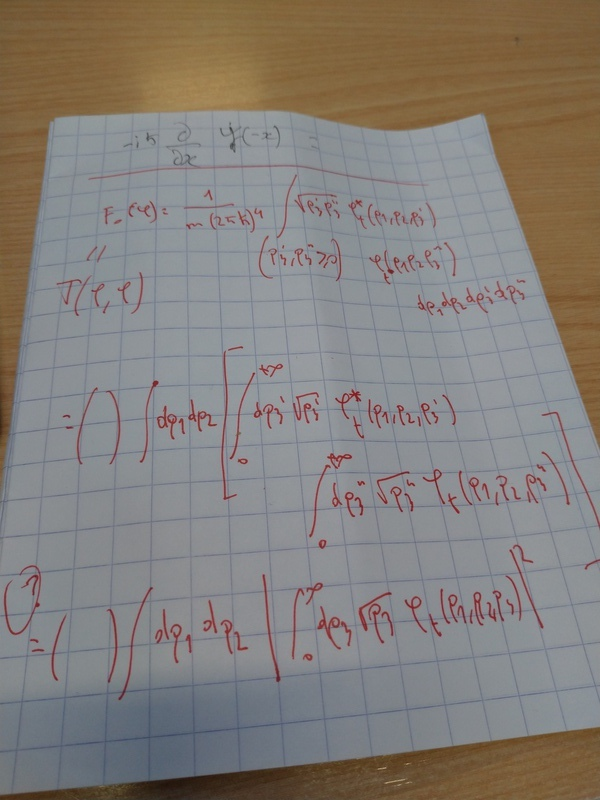
\includegraphics[width=\linewidth]{img/tmp/kijowski1.jpg}

\section{Detector models}\label{sec:hist:detect}

One of the considerations we can gather from the previous Sections
is that 
the problem of arrival time ---of a particle at a particular region of space---
can be tackled at differemt ``levels''. 

Operationally, there must be a detector which
``clicks'' at the arrival of the particle, and the statistical distribution of
such click times over repeated measurements is studied. Due the Pauli objection,
probabilities in this distribution cannot simply be given in terms of projectors related to eigenspaces of a self-adjoint operator.
A more general formulation than projective measurement is therefore necessary.

Detectors can be treated more or less explicitly in quantum models of arrival time:
\begin{enumerate}
  \item
    Without making the detector explicit. This is the case of the Kijowski model (Sec. \ref{sec:kijowski}),
    which is based on positive-operator measurement (POVM). Given there's no detector in the model,
    the best candidate statistical distribution and operator are essentially obtained
    through consistency arguments including a reasonable classical limit.
  \item
    Early attempts at incorporating the measurement apparatus
    (namely Allcock, Sec. \ref{sec:allcock}) which
    focus on the irreversible process of absoption.
    Normalization of the quantum state is not preserved, the Hamiltonian is not Hermitian
    because the potential is not real. The rate of normalization-loss is interpreted as
    absorption (detection, arrival) probability over time. The detector is in fact
    ``traced out'' and the particle is treated as an open system (Sec. \ref{sec:halliwell}).
  \item
    Full detector models. For example the Atom-Laser one. Two-level atoms in the ground state
    are sent to a laser-illuminated region (we're interested in the time-of-arrival into this region),
    get excited, and the first photon which is spontaneously emitted following the excitation
    is interpreted as detection of the arrival in the region. Problems related to
    reflection, low absorption rate, and delay in the spontaneous emission are fully taken into account in the model.
\end{enumerate}

A brief, mostly qualitative, illustration of the Atom-Laser model is
given below, and references therein can be consulted for more details.

\subsection{Basics of Atom-Laser Model}

As pointed out in \cite{Damborenea}, the model by Halliwell (Sec. \ref{sec:halliwell})
has the merit of including irreversibility in the detection process,
but ``remains somewhat abstract
since no connection is made with any specific measuring
system''. The work by Damborenea et al. \parencite{Damborenea} gives instead an operational
description of arrival time.

In its essence, the model describes an atom sent to a laser-illuminated region,
of which the arrival time into the region is taken as the time\footnote{
  Please note, while there is an operational definition of detection,
  there is no operational definition of time, in other words,
  while this model does include an explicit description of the detector,
  there is still no description or definition of a ``clock'',
  which is still somewhat implicitly assumed as a ``classical'' one.
  This further motivates theories modelling quantum clocks instead,
  as seen from Chapter \ref{ch:pw} on.
}
when the first photon is spontaneously emitted by the atom itself,
following its excitation by the laser.
The spontaneous photon emission is therefore the ``click'' of the detector.

This time-of-arrival formulation has been shown in excellent numerical agreement
with Kijowskii axiomatic distribution.

One limitation of the model is given by delays:
\begin{enumerate*}[label=\arabic*)]
  \item in the transition of the atom to the excited state, and
  \item in the spontaneous emission.
\end{enumerate*}
This cannot be addressed by simply increasing the laser intensity
(therefore shortening the excitation and decay time)
because this would lead to elastic reflection,
and the most likely outcome would be no detection/absorption at all.
This is similar to the issue encountered, at a teorethical level,
by Allcock when the imaginary absorbing potential was too large.

A suitable detector configuration, therefore, will be based on ``weak driving'',
but will need the delays to be compensated via
a convolution with an atom at rest.

* solution: deconvolution with an atom at rest to subtract the delay: with shorter lifetimes converges to probability current (at $x=0$ towards the right?)

* the above convergence is just a proof of reasonability, because we still want to avoid too short lifetimes for reflection, right?

* a way to implement this experimentally is actually by a 3-level system, a middle metastable ``sink'' state after emission so atome can't be excited again: this motivates studying 3-level systems with PW later; see \cite{Metastable}.

* eq. 4.7 in book, brief mention on how the simplification is obtainied, detuning, on-resonance, so Delta is zero.

* a particular case of it goes on next section (where Kiukas et al heavily cited)

* what params makes little reflection but good prob. of detection?

* fig. 4.3 in book, discrete points, delay (convolution etc.), sec. 4.2.2 book

* in next section we don't care of delay because we study the time of decay rather than the time of arrival of the atom (or we assume they coincide because convolution technique was used).

* $\Pi$ is loss of normalization

\subsection{Ruschhaupt, Kiukas et al}\label{sec:hist:detect:kiukas}

Studies
about detector models which investigate
time-of-arrival as a quantum observable.
In particular we consider \cite{RuschhauptAbsorption},
which in turn traces back its basic ideas from the seminal work by Allcock
in the 1960s \parencite{Allcock-1, Allcock-2, Allcock-3},
while a detailed contemporary formulation can be found in
\cite[Ch. 4]{TQM2}.

A non hermitian Hamiltonian is justified as a computation method
to simplify the study of some open systems: the evolution of mixed
states is derived without explicit reference to density operators
or master equations, but resolving equations that are formally
identical to those of pure states,
i.e. in terms of
Schr{\"o}dinger equations and wave functions,
with the non-hermitian term in the Hamiltonian
to account for the non-unitarity of the evolution.

The detection-by-absoption model in \cite{RuschhauptAbsorption}
is based on a complex potential that, plugged into the Schr\"odinger equation,
leads to a non-unitary evolution of the state vector
(with loss of normalization).

Specifically, the Hamiltonian $\hat{H}$ is replaced by a $\hat{H} - i\hat{D}$
(with $\hat{D}$ self-adjoint, bounded, positive)
and, consequently:
\begin{equation}\label{eq:schrod_complex_pot}
  \hat{H} \ket{\psi(t)} = i\hbar\dv{t}\ket{\psi(t)} +i\hat{D}\ket{\psi(t)} \text{.}
\end{equation}

\citereset\subsection{Application: two-level system}

In \cite{RuschhauptAbsorption}, an example application of the detector model
is provided for a two-level system.
In Page and Wootters terms,
this would corrspond to a bi-dimensional $\hilb{H}_S$, but a continuous
spectrum of $\hat{T}$ in $\hilb{H}_T$. The paper is \emph{not} based on
the Page--Wootters model, indeed the purpose of this section is a comparison
with such model, using the results of Section \ref{sec:absorption+pw}.

By setting, out of convenience, $\hbar = \omega = 1$
(with $\omega$ the characteristic frequency of the system),
and directly considering the parameters
that minimize the time--energy uncertainty product \parencite{RuschhauptAbsorption},
we have a non-Hermitian ``Hamiltonian''
$\mathit{K} = \hat{H} - i\hat{D}$ with
\begin{equation}\label{eq:complexpot}
  \mathit{K} = \hat{H} - i\hat{D} \repr
    \hbar\omega\left\{
      \left[\begin{matrix}0 & 1\\1 & 0\end{matrix}\right] -
      i \left[\begin{matrix}0 & 0\\0 & \gamma \end{matrix}\right]
    \right\}
\end{equation}
and $\gamma = 2\sqrt{2}$.

We take an initial state of $\ket{0}$
(or $\mqty[1\\0]$ in matrix form).

We then compute, symbolically, the non-unitary evolution
$\ket{\psi(t)} = e^{-i\mathit{K}t}\ket{0}$
with the aid of \term{SymPy} \parencite{comp:sympy} within a \term{Jupyter} \parencite{comp:jupyter} notebook
(see Appendix \ref{detector-model-kiukas-ruschhaupt-schmidt-werner} for all the details of the calculation).

Simplifying the result in eq. \eqref{eq:sympy:non-unitary-evol}, we have:
\begin{equation}
  \ket{\psi(t)} \repr e^{-\frac{\sqrt{2}}{t}} \mqty[
    \cos(\frac{\sqrt{2}}{2}t) + \sin(\frac{\sqrt{2}}{2}t)& \\
                     -i\sqrt{2} \sin(\frac{\sqrt{2}}{2}t)&
  ] \,\text{.}
\end{equation}

\begin{figure} %% https://tex.stackexchange.com/a/165730
  \centering
  \begin{subfigure}{0.49\textwidth}
    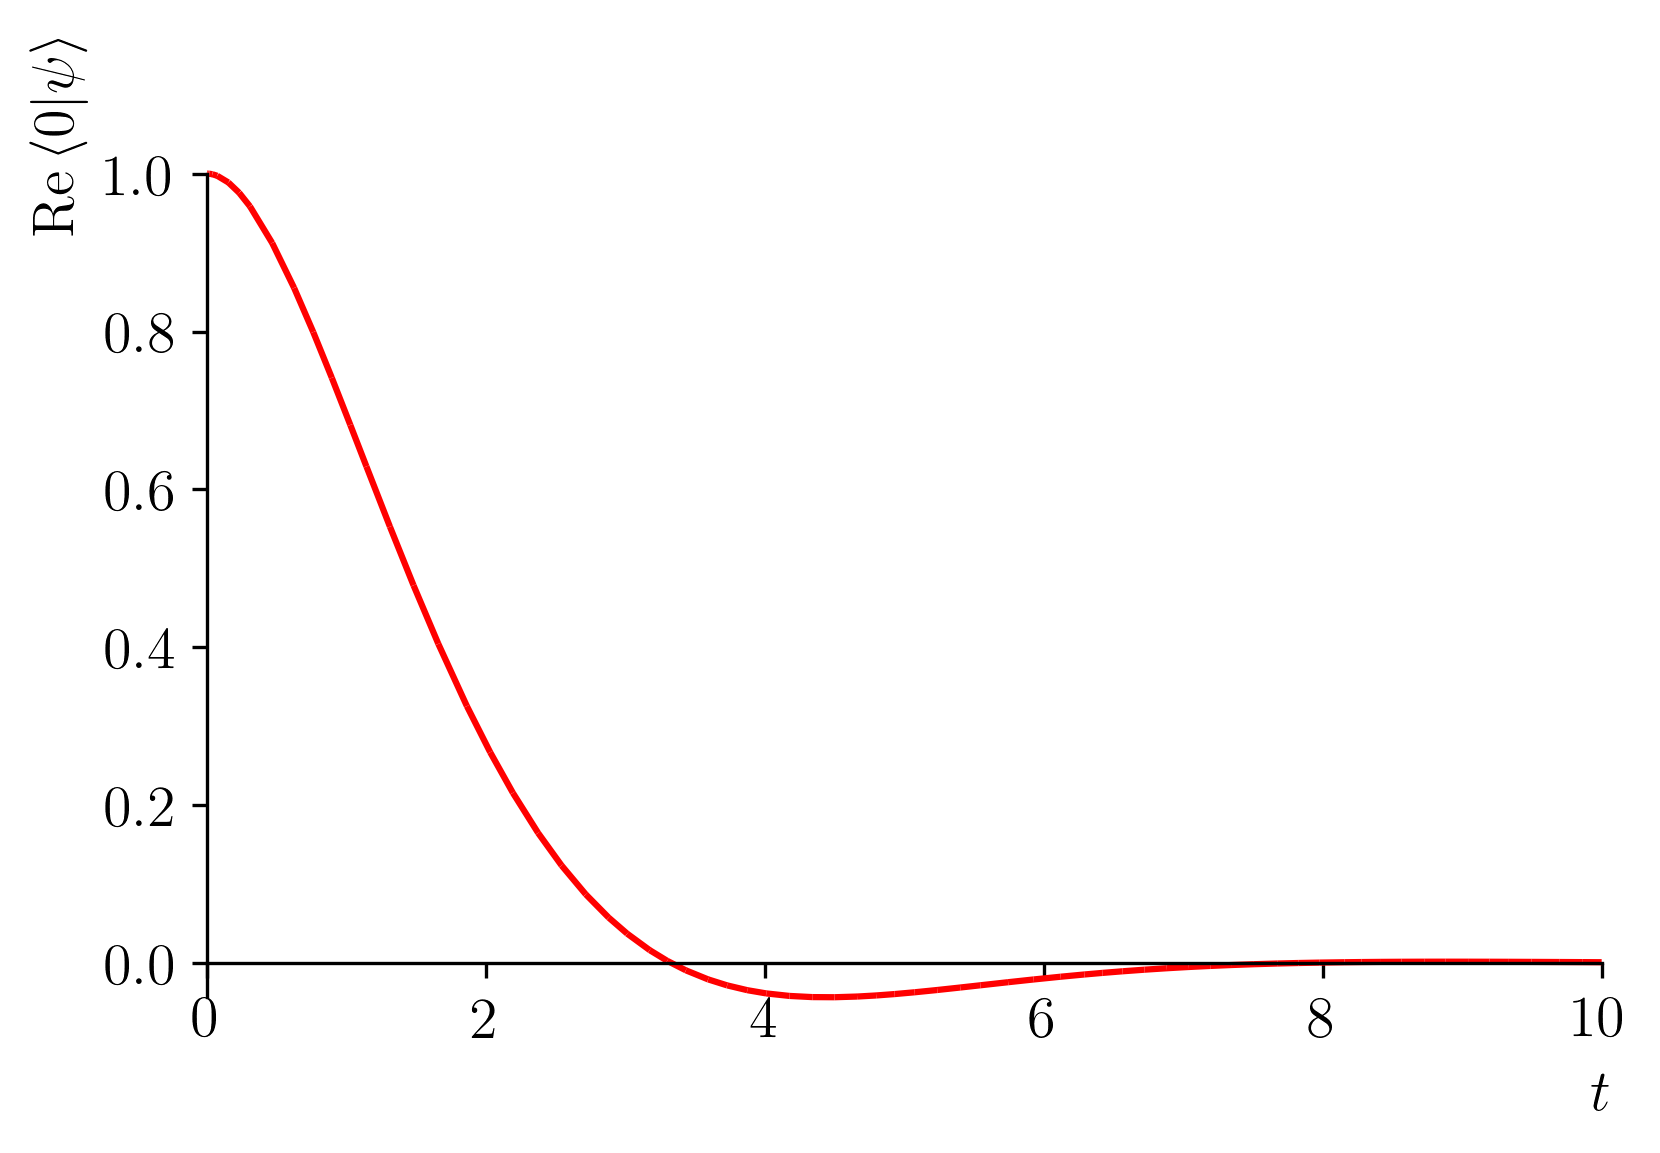
\includegraphics[width=\linewidth]{img/2ldetect/re_psi0_t.png}
    \subcaption{}\label{fig:absorbed-qubit-components:re0}
  \end{subfigure}
  % \hspace*{\fill} % separation between the subfigures
  \begin{subfigure}{0.49\textwidth}
    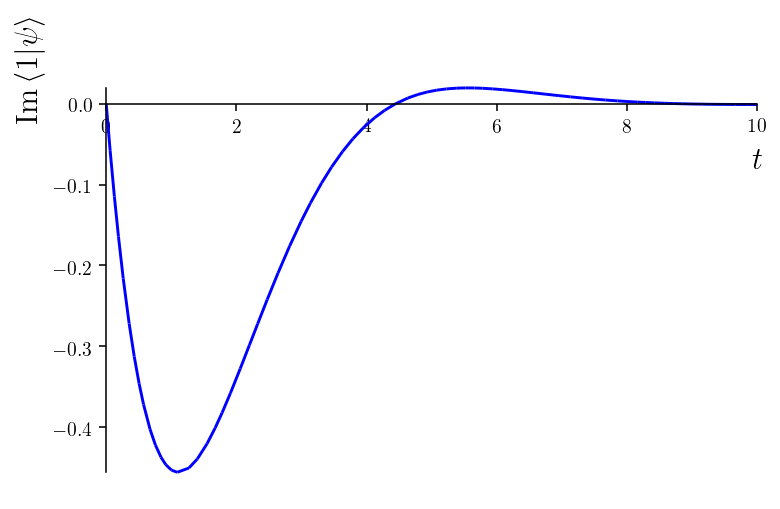
\includegraphics[width=\linewidth]{img/2ldetect/im_psi1_t.png}
    \subcaption{}\label{fig:absorbed-qubit-components:im1}
  \end{subfigure}
  % \hspace*{\fill} % separation between the subfigures
  \caption{
    Non-unitary evolution of the absorbed qubit
    according to the model in
    ref. \cite[sec.``Emission from a two-level system'']{RuschhauptAbsorption}.
    The component along $\ket{0}$ is purely real,
    and the one along $\ket{1}$ is purely imaginary,
    therefore only their their respective parts are plotted.
  }\label{fig:absorbed-qubit-components}
\end{figure}

\begin{figure}
  \centering
  \begin{subfigure}[b]{0.49\textwidth}
    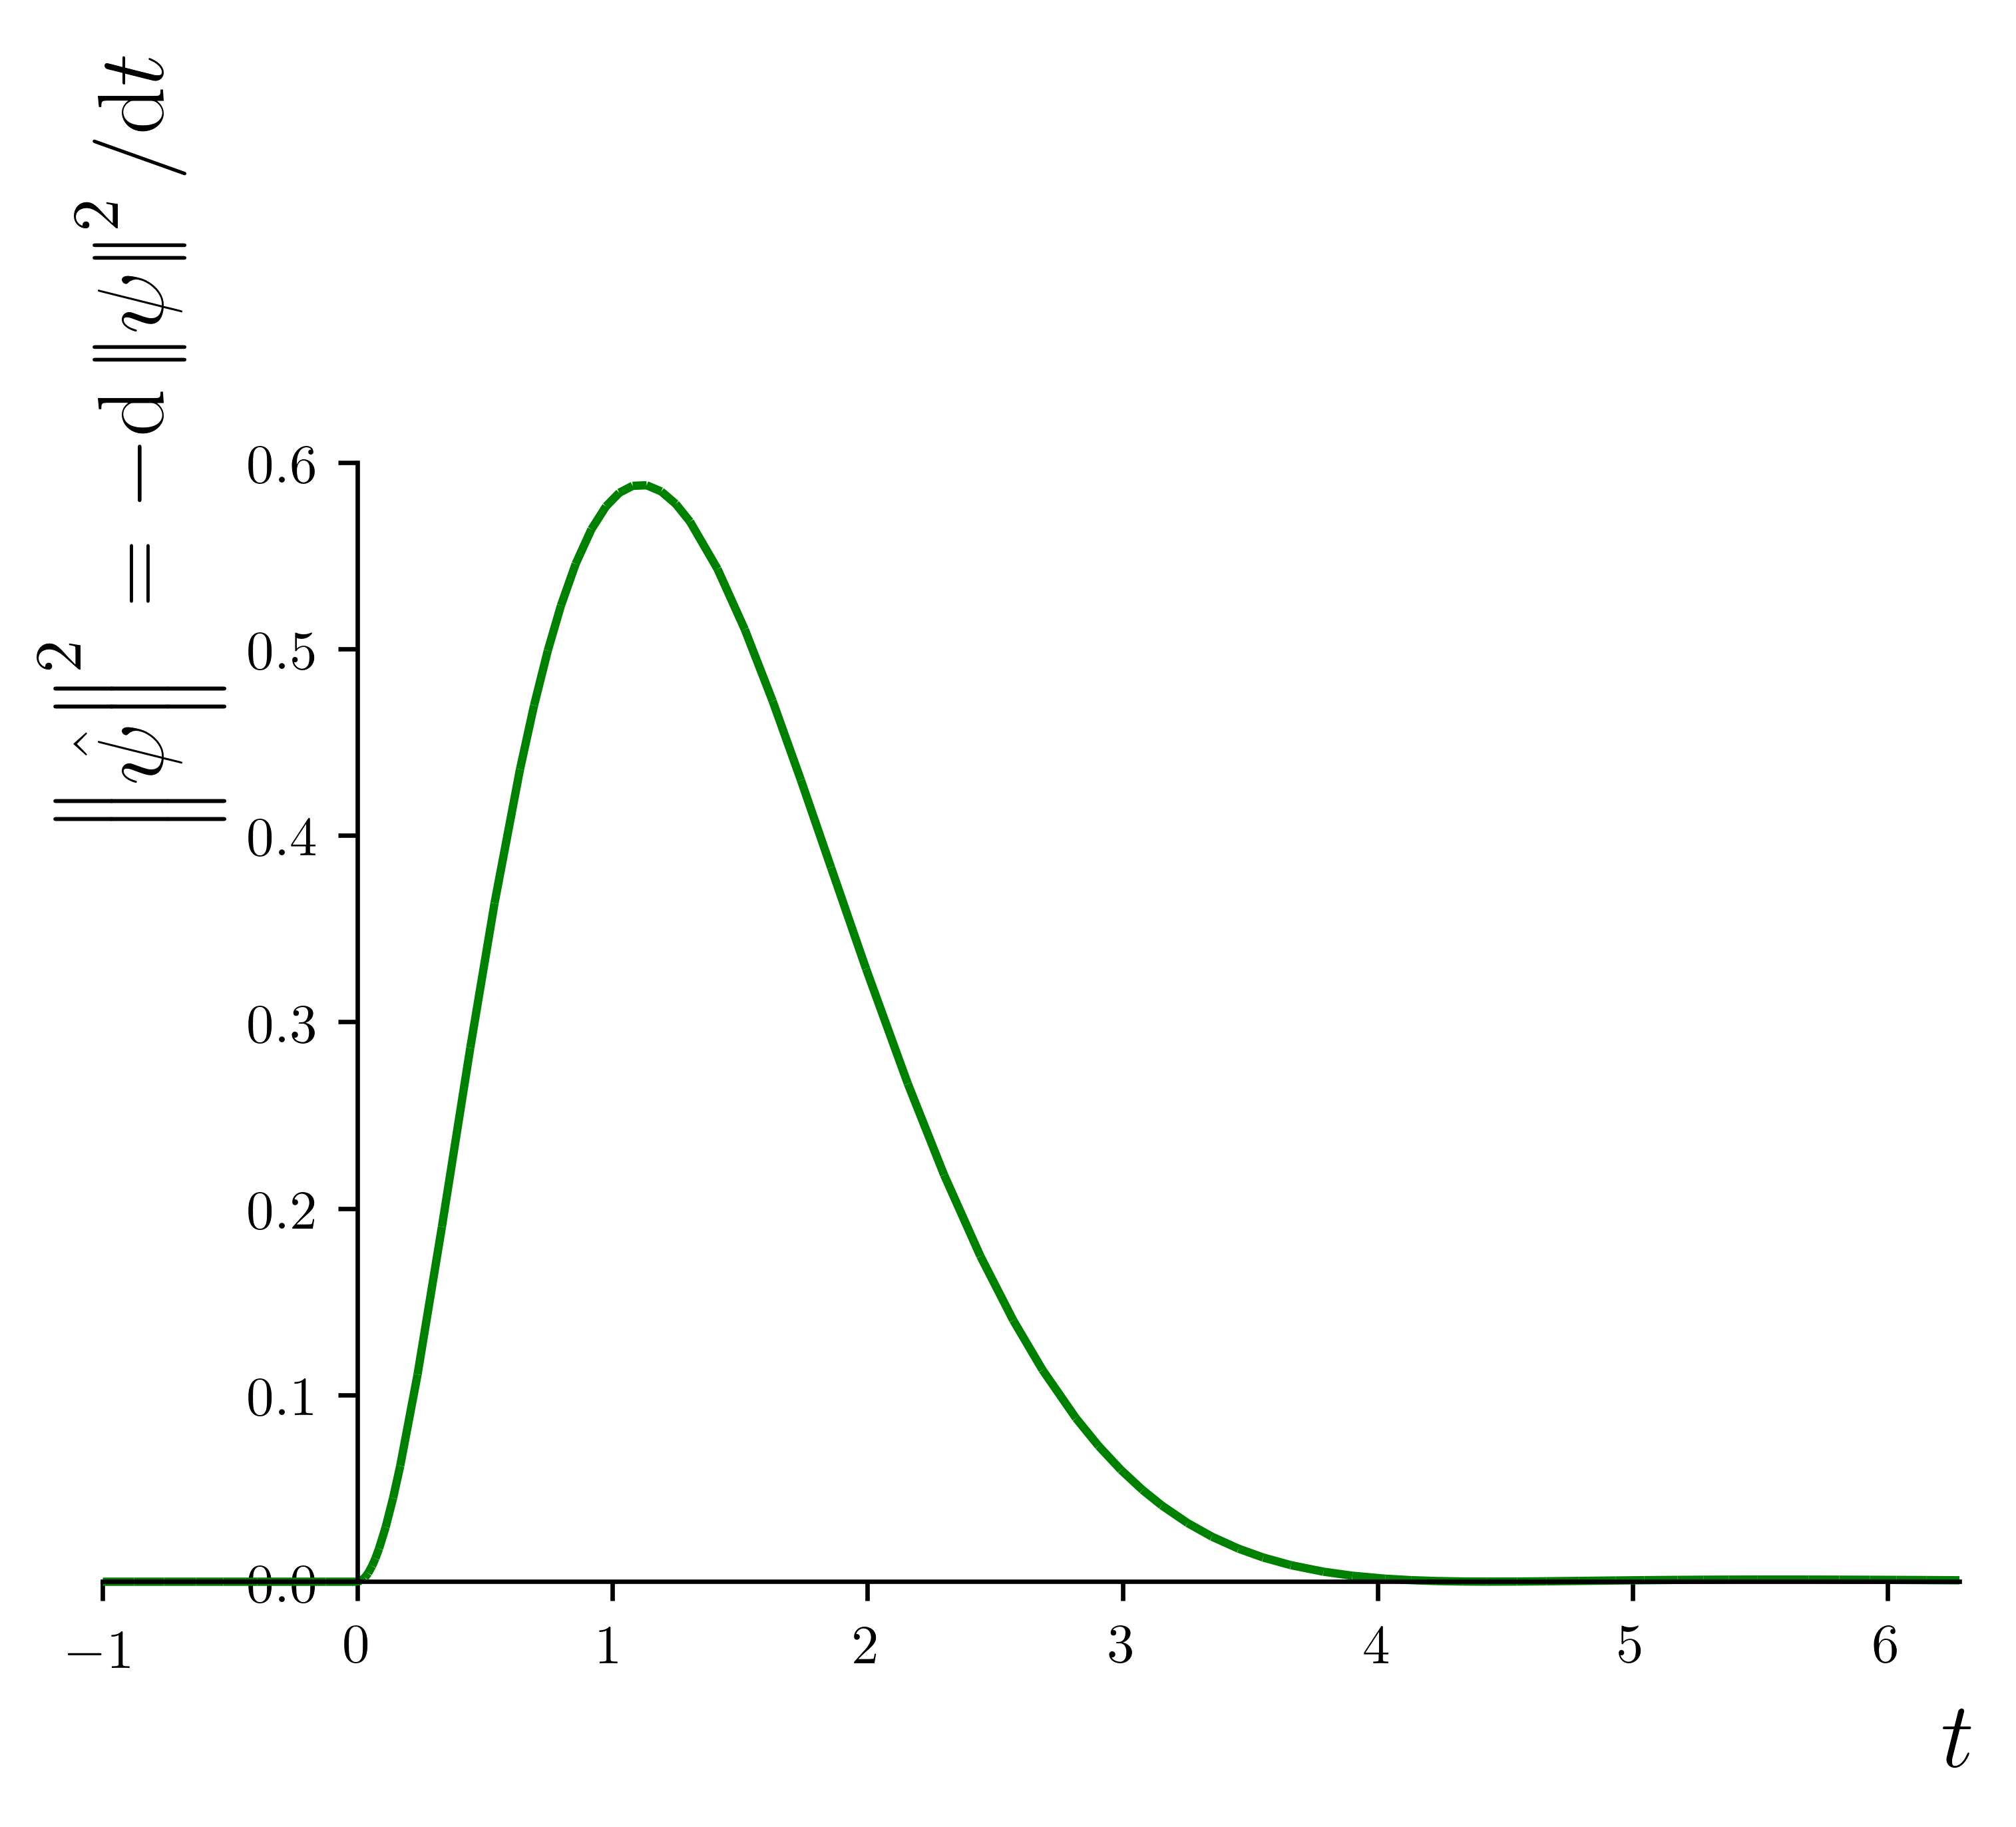
\includegraphics[width=\linewidth]{img/2ldetect/qubit_normalization_loss.png}
    \subcaption{}\label{fig:absorbed-qubit-normalization-loss:t}
  \end{subfigure}
  \begin{subfigure}[b]{0.49\textwidth}
    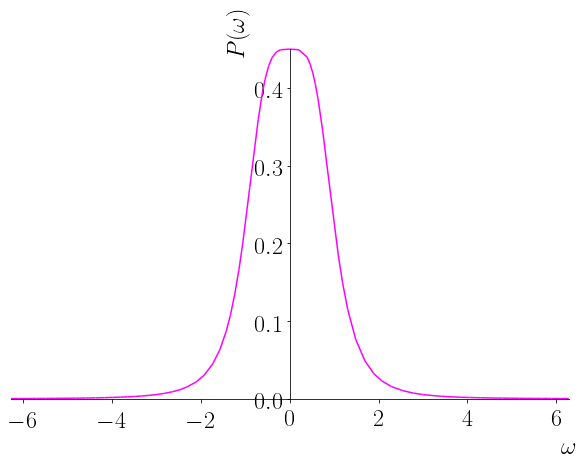
\includegraphics[width=\linewidth]{img/2ldetect/P_omega.png}
    \subcaption{}\label{fig:absorbed-qubit-normalization-loss:omega}
  \end{subfigure}
  \caption{
    Non-unitary evolution of absorbed qubit.
    \subref{fig:absorbed-qubit-normalization-loss:t}
      Detection probability in time. It's equal to the
      loss of normalization $-\dv{\norm{\psi}^2}{t}$
      (but also to the squared norm of $\hat{\psi}(t)$ as of eq. \eqref{eq:analytic:hatpsi}.
    \subref{fig:absorbed-qubit-normalization-loss:omega}
      Detection probability in the frequency domain.
  }
  \label{fig:absorbed-qubit-normalization-loss}
\end{figure}

The ``lossy'' evolution, with the two components of the qubit, is shown in Fig.~\ref{fig:absorbed-qubit-components}.
The loss of normalization $-\dv{\norm{\psi}^2}{t}$, indicating the probability of detection by absorption,
is then derived directly and shown in Fig.~\ref{fig:absorbed-qubit-normalization-loss}.

This yields the \emph{probability} of detection.
One may wonder whether it is possible to derive a corresponding \emph{probability amplitude} vector,
whose squared norm across time is equal to the said probability distribution.\footnote{
  The solution is of course not unique, but one may ask whether such functions would lead
  to quantum interference patterns and other phenomenology which may be subject of further study.
}
Within the framework of \cite{RuschhauptAbsorption}, a ``wavefunction in time'' in such sense
is the $\hat{\psi}$, as in \eqref{eq:phi_psi_kiukas}.
It is computed in detail within the
notebook in Appendix \ref{detector-model-kiukas-ruschhaupt-schmidt-werner}, eq. \eqref{eq:sympy:hatpsi},
simplifying which we obtain:
\begin{equation}\label{eq:analytic:hatpsi}
  \hat{\psi}(t) =
    i 2^{\frac{5}{4}} e^{-\frac{\sqrt{2}}{2}t}\sin(\frac{\sqrt{2}}{2}t) \theta(t)
    \ket{1}
    \text{,}
\end{equation}
with $\theta(t)$ the Heaviside step function.

\begin{remark}\label{remark:detection_area}
In general, the operator $\hat{D}$ as in \eqref{eq:schrod_complex_pot}
is such that the eigenspace corresponding to its zero eigenvalue
is the ``area'' where the detector is not sensitive. Or, in other words,
the linear span of states with zero probability of triggering the detector.
Therefore, when $\hat{D}$ (or its square root) is applied to a state vector,
for example in \eqref{eq:phi_psi_kiukas},
the components in such eigenspace are cut off and the resulting
$\hat{\psi}$, eq. \eqref{eq:analytic:hatpsi} in the example, lies at all times in the ``area of detection''
i.e. it's a multiple of $\ket{1}$ in this case.
\end{remark}

The corresponding Page--Wootters (proper) vector of $\pwspace$ is
\begin{equation}\label{eq:hatpsi:pw}
  \dket{\Phi} = \int \dd{t} \ket{t} \ox \hat{\psi}(t) \,\text{,}
\end{equation}
to which the considerations of Section \ref{sec:for-normalized-elements}
and Section \ref{sec:pure-state-approach} in terms of time--frequency
(or time--energy) uncertainty relation apply, with some analogy
to what \cite{RuschhauptAbsorption} does within its own framework
in relation to $\hat{\psi}$ and its Fourier transform.

In that regard, the \eqref{eq:hatpsi:pw} can be reformulated
\begin{equation}
  \dket{\Phi} = \int \dd{\omega} \ket{\omega} \ox \mathcal{F} \hat{\psi} (\omega) \,\text{,}
\end{equation}
where it's
\begin{equation}
  \mathcal{F} \hat{\psi} (\omega) = - \frac{\sqrt[4]{2} i}{\sqrt{\pi} \left(- \omega^{2} + \sqrt{2} i \omega + 1\right)} \ket{1}
\end{equation}
---see notebook up to eq. \eqref{eq:fhatpsi1_omega} for details.

Taking the squared modulus, a probability distribution over angular frequency
(or, equivalently, energy) is obtained:
\[
  P(\omega) = \frac{\sqrt{2}}{\pi \left(\omega^{4} + 1\right)}
  \,\text{.}
\]
See Fig. \ref{fig:absorbed-qubit-normalization-loss:omega}.

\chapter{Page and Wootters Relational Time}\label{ch:pw}\label{ch:detect}
% formalism
% \subsection*{\it Structure of the Chapter}

This Chapter
will be devoted to outlining the Page and Wootters theory
of time,
also known as the model of ``evolution without evolution''.
Existing literature will be reviewed,
with some original considerations,
in particular with regards to
time--energy uncertainty relations,
finite-dimensional systems and discrete clocks
(Sections \ref{sec:pw:theory_first}--\ref{sec:pw:theory_last}).

A second part
(Sections \ref{sec:pw:apps_first}--\ref{sec:pw:apps_last})
will be dedicated to
applications of the Page--Wootters model, starting with a discussion of existing
experiments (or ``experimental illustrations''),
then implementing numerical simulations, with a larger number of clock levels.
Finally, the Page and Wootters model will be compared to the results of
detection and time-of-arrival models
based on non-unitary evolution.

\section{The Model}\label{sec:pw:theory_first}

To introduce the Page--Wootters model, let us first consider
a bipartite system $\hilb{H}_T \ox \hilb{H}_S$,
and a state vector $\dket{\Psi} \in \pwspace$.
%% Move to finite-dim section? is this just a redundant repetition?
% the two subsystems of which have finite dimension\footnote{
%   In general, within the model,
%   the system may as well be infinite-dimensional;
%   the sum may be replaced by an integral (continuous spectrum);
%   and the vector in the tensor-product space may be not normalizable (an improper vector).
%   Nonetheless, a finite-dimensional Hilbert space is sufficient to construct several applications of interest.
% } $N$ each.
% Let us also consider the following entangled state:
% \begin{equation}\label{eq:pw:finite-entanglement}
%   \hilb{H}_T \ox \hilb{H}_S \ni \dket{\Psi}
%   =
%   \frac{1}{\sqrt{N}} \sum_{n=0}^{N-1} \ket{\tau_{n}}_{T} \ox \ket{\psi_{n}}_{S} \text{.}
% \end{equation}
A ``double angle bracket'' notation $\dket{\Psi}$ is used here
for vectors in the tensor product space.
% We assume that $\ket{\psi_{n}}_{S}$ are all \emph{normalized} in $\hilb{H}_S$;
% and
% $\qty{\ket{{\tau}_n}}$ is an orthonormal eigenbasis of some observable (say, $\op{T}$)
% in $\hilb{H}_T$.
% Furthermore,

Let $\dket{\Psi}$ be \emph{stationary}, meaning it is an eigenstate
of an overall Hamiltonian $\op{\mathbb{J}}$ in $\hilb{H}_T \ox \hilb{H}_S$:
\begin{equation}\label{eq:Wheeler-DeWitt}  %%  eq:Wheeler-DeWitt + eq:pwHamiltonian
  \op{\mathbb{J}} \dket{\Psi} = 0 \text{.}
\end{equation}
Finally, we assume that the two subsystems
are \emph{non interacting},
meaning that the global Hamiltonian $\mathbb{J}$ can be expressed as a sum of two terms
which only act on the respective subspaces $\hilb{H}_T$ and $\hilb{H}_S$
(and there is no explicit ``interaction term''). In other words,
$\op{\mathbb{J}}$ can be expressed as
\begin{equation}\label{eq:pwHamiltonian}
  \op{\mathbb{J}} = \op{H}_T \ox \idop_S + \idop_T \ox \op{H}_S \, \text{.}
\end{equation}
Therefore,
the evolution of the subsystem described by $\hilb{H}_S$
will only depend on ``its own''
Hamiltonian $H_S$ (assumed as time-independent), namely
\begin{equation}\label{eq:pw:ordinary_S}
  \ket{\psi(t)}_S = e^{- i \op{H}_S t / \hbar} \ket{\psi(0)}_S \text{.}
\end{equation}
Note the familiar single-bracket notation $\ket{\psi(t)}_S$ for a ket in
one of the two parts (subspaces) of $\pwspace$ ($\hilb{H}_S$ in this case).

The overall bipartite system is \emph{isolated}. A notable example of isolated system is, of course, the universe.
This simple observation is relevant because,
in its original formulation \parencite{PageWootters}, $\pwspace$ is regarded
as a partition of the whole universe, which is considered, overall, in a stationary state.
% There cannot be notion of time external to it.

This is known as the
``timeless'' approach \parencite{Marletto:Evolution}.
\citereset
A suitable subsystem ---described by $\hilb{H}_T$ within this framework---
is chosen in the ``universe'' so that it acts as
\emph{clock} for the \emph{rest} of it, in the sense that
there is an observable $\op{T}$
which can be used to
describe the time evolution ``without evolution''
of the other subsystem\footnote{
  A slightly different notation
  uses indeed $\hilb{H}_C$ and $\hilb{H}_R$ (instead of $\hilb{H}_T$ and $\hilb{H}_S$)
  to indicate the Hilbert spaces of the clock~(C) and the rest~(R) of the ``universe''
  (or isolated system):
  see, for example, \cite{Marletto:Evolution}.
}
$\hilb{H}_S$.

The operator $\op{T}$ can be regarded as
the \emph{time operator}. It is defined in $\hilb{H}_T$ (not $\hilb{H}_S$),
and canonically conjugate to the ``Hamiltonian'' $\op{H}_T$ (not $\op{H}_S$).
In other words, the time operator is defined in a different Hilbert space than the ``system of interest'' $\hilb{H}_S$,
therefore
the Pauli objection (Sec.~\ref{proof}) no longer applies.

As we will see below, in the Page--Wootters model, time evolution is based on an internal \emph{entanglement}
relation among elements of subspaces $\hilb{H}_S$ and $\hilb{H}_T$ respectively.

% Quantitatively,
% the observable $T$ in $\hilb{H}_T$
% has eigenvalues $\tau_n$
% (assuming a discrete spectrum to simplify notation)
% which can be interpreted as possible
% instants of time in the evolution of $\ket{\psi}_S$, in the sense that
% \begin{equation}\label{eq:pw:discrete_Tpprox}
%   \Big[ \ket{\psi(t)}_S \Big]_{t=\tau_n} = \,\,\,\, \ket{\psi_n}_S \, \text{,}
% \end{equation}
% where $\ket{\psi(t)}_S$ is given in~\eqref{eq:pw:ordinary_S} i.e.
% the evolution one would obtain in ``ordinary'' way
% by resolving the Schr\"{o}dinger equation in $\hilb{H}_S$.
% Please note:
% in its original formulation, the Page--Wootters model is based on a continuous
% notion of time, and the same applies to more recent developments \parencite{Lloyd:Time}.
% A discrete formulation, as in Eq.~\eqref{eq:pw:discrete_Tpprox},
% will be verified numerically in Sections~\ref{sec:beyondMoreva}--\ref{sec:multiLevelClock}.

An intuitive description may be as follows.
From the perspective of the system described by $\hilb{H}_S$,
time is a parameter $t$;
however $t$ can have values
which are also eigenvalues of an observable $\op{T}$ defined in \emph{another} space $\hilb{H}_T$,
with which it is entangled. Such entanglement relation establishes a correspondence
between ``instants of time'' (eigenvalues and eigenstates of observable $\op{T}$)
and (``evolved'') states in $\hilb{H}_S$.

%%
%% \section{Development of the Formalism}\label{sec:pw:formalism}\label{sec:pw:theory_first}
%%

About three decades after the original work
by Page and Wootters \parencite{PageWootters},
the formalism was developed further
by Giovannetti, Lloyd and Maccone \citereset\parencite{Lloyd:Time}.
Most technical details introduced below are based
on that paper.

First of all, the ``conventional'' state $\ket{\psi(t)}_S$ in $\hilb{H}_S$
can be obtained from $\dket{\Psi}$ via partial inner product\footnote{
  For the partial inner product,
  see Definition \ref{def:pBra} and \ref{def:pKet},
  and \cite[\s 1.3.3]{QMT_Jacobs}.
}
with a time eigenstate $\prescript{}{T}{\bra{t}}$:
\begin{equation*}
  \ket{\psi(t)}_S = \prescript{}{T}{\bradket{t}{\Psi}} \, \text{.}
\end{equation*}
The function $ t \rightarrow \ket{\psi(t)}_S \; $ is the
``wavefunction in time representation'', in analogy
with the wavefunction in position representation of standard quantum mechanics.
The state vector $\dket{\Psi}$ is univocally identified by the ``coefficients'' $\ket{\psi(t)}_S$
with respect to the basis $\setof{\ket{t}_T}$:
\begin{equation}\label{eq:pw:}
  \dket{\Psi} = \int \dd{t} \ket{t}_T \ox \ket{\psi(t)}_S \, \text{,}
\end{equation}
somewhat similar to the well known expression $\ket{\psi}_S = \int \dd{x} \psi_{S}(x) \ket{x}_S$
which defines the position representation.

Under this time representation (or T representation), the operator $\op{H}_T = -\hbar\op{\Omega}$,
canonically conjugate to the time operator $\op{T}$, is expressed as $-i\hbar\pdv{t}$,
and the commutation relation
$[\op{T}, \op{H}_T] \repr[T] \comm{t, -i\hbar\pdv{t}}{} = i\hbar$
can be proven
immediately, similarly to the well known position-momentum relation
$\comm{\op{x}}{\op{p}} \repr[x] \comm{x}{-i\hbar\pdv{x}} = i\hbar$.
Thus, $\hbar\op{\Omega}$ can be seen as similar to a ``linear momentum''
in the Hilbert space of time.

%% \hbar\Omega is -E ... and \Omega \repr -i t-derivative ... and [T, \Omega] = i .

Using the $T$ representation in $\hilb{H}_T$,
and comparing \eqref{eq:pwHamiltonian} and \eqref{eq:Wheeler-DeWitt}:
\begin{equation}\label{eq:schrod_from_pw}
  0 = \qty(\hbar\op{\Omega}\ox\idop_S + \idop_{T}\ox\op{H}_S)\dket{\Psi}
    \repr -i\hbar\pdv{t}\ket{\psi(t)}_{S} + \op{H}_S\ket{\psi(t)}_{S}
    \,\text{,}
\end{equation}
we recover the usual form of the Schr\"{o}dinger equation in $H_S$
(see also \cite[709--710]{Wootters:Loyola}).

Here $\op{\Omega}$ can be seen as a ``frequency operator''
represented as $i\pdv{t}$ and having as eigenfunctions
those functions evolving in time with a phase factor $e^{i \omega t}$ only.

From another point of view, $\op{H}_{T} = \hbar\op{\Omega}$ is the ``Hamiltonian'' of $\hilb{H}_T$,
in that it plays a similar role of $H_S$ in the construction of
$\op{\mathbb{J}}$ in \eqref{eq:pwHamiltonian}.

Such analogies among operators in $\hilb{H}_T$ and $\hilb{H}_S$ are summarized in Table \ref{tbl:op_comparison_pw}.

{
  %% https://tex.stackexchange.com/a/232874
  %% https://tex.stackexchange.com/a/2836
  \begin{table}
    \centering
    \begin{tabular}{l|l|l}
      & \multicolumn{1}{c|}{$\hilb{H}_T$}                 & \multicolumn{1}{|c}{$\hilb{H}_S$}       \\
      \hline
      \multirow{2}{11em}{Canonical commutation relation}
      & $\op{T}$                                          & $\op{x}$                            \\
      %
      & $\op{H}_T \repr[T] -i\hbar\pdv{t} $  & $\op{p} \repr[x] -i\hbar\pdv{x}$       \\
      \hline
      Hamiltonian
      & $\op{H}_T$                                        & $\op{H_S}$
    \end{tabular}
    {\caption{
      Analogies between observables in the two Hilbert spaces.
    }\label{tbl:op_comparison_pw}}
  \end{table}
}

% It would be interesting to a study relativistic extension of the
% Page and Wootters model that allows, for example, the derivation of the Klein-Gordon
% equation, thus eliminating the asimmetry between
% $\hilb{H}_T$ and $\hilb{H}_S$ (and momentum and energy as well).

In the bipartite universe, physical kets $\dket{\Psi}$ can have a Schmidt decomposition
made up of
eigenstates $\ket{\omega}_{T}$ of $\op{H}_T$ in $\hilb{H}_T$
entangled with
eigenstates $\ket{\tilde{\psi}(\omega)}_{S}$ of $\op{H}_S$ in $\hilb{H}_S$
(the eigenvalue is $\hbar\omega$ for both $\op{H}_T$ and $\op{H}_S$ respectively);
or eigenstates $\ket{t}_{T}$ of $\op{T}$ in $\hilb{H}_T$
entangled with time-evolved spatial states~$\ket{\psi(t)}_S$ in $\hilb{H}_S$:
\begin{equation}\label{eq:pw:time_freq_nomu}
  \dket{\Psi} =
    \int \dd{\omega} \, \ket{\omega}_{T}\ox\ket{\tilde{\psi}(\omega)}_{S} =
    \int \dd{t} \, \ket{t}_{T} \ox \ket{\psi(t)}_{S} \text{.}
\end{equation}
%
% \begin{tcolorbox}
%   Eq.~\eqref{eq:pw:time_freq_mu} here is based on \cite[eq. 10]{Lloyd:Time}.
%   The paper, in the first integral,
%   would use a ``measure'' $\dd{\mu(\omega)}$, instead of simply $\dd{\omega}$.
%   This is to take into account that not all values of $\omega$ necessarily contribute
%   to the integral: in particular if $\hbar\omega$ is not in the spectrum of $\op{H}_S$,
%   the corresponding integrand would be zero.
%
%   So,
%   I can certainly remove $\dd{\mu(\omega)}$ as requested\footnote{
%     I actually even wrote $\dd{\omega}\mu(\omega)$ in my previous draft,
%     somewhat incorrectly:\linebreak
%     technically I should have written $\dd{\mu(\omega)}$,
%     or $\dd{\omega}\mu'(\omega)$ (with a ``prime'')
%     so that $\dd{\mu(\omega)} = \frac{\dd{\mu}}{\dd{\omega}}\dd{\omega} = \mu'(\omega) \dd{\omega}$
%     to match the paper,
%     but that's probably not the most important point here\dots
%   },
%   and simply write $\dd{\omega}$, but at least I need to specify what follows:
%   %
%   that, while it is $\braket{\psi(t)}_S = 1 \ \forall t \in \mathbb{R}$
%   (unitary evolution, as in standard~QM),
%   one should not necessarily expect that
%   $\ket{\phi(\omega)}_S$ has norm $1$ for every real value of $\omega$.
%   Actually, given that the spectrum of $\op{H}_S$ is bounded from below,
%   certainly there are values of $\omega$ for which $\ket{\phi(\omega)}_S = \nullvector$.
%
%   In other words, we can certainly remove $\mu(\omega)$, but it must be ``absorbed''
%   in the properties of $\ket{\phi(\omega)}_S$.
% \end{tcolorbox}

Using the relations
$
\, \prescript{}{T}{\braket{t}{t'}}_T = \delta(t-t') \,
$
and
$
  \,
  \ket{\omega}_T =
  \frac{1}{\sqrt{2\pi}} \int\dd{t}\E^{-\iu\omega t}\ket{t}_T
  \,
$
(see also \cite[2]{Lloyd:Time}),
it follows that\footnote{%
  Please note the analogy with the well-known
  inner product of position and momentum eigenvectors in standard quantum mechanics:
  $\braket{\vb{x}}{\vb{p}} = (2\pi\hbar)^{-3/2}\E^{\iu \vb{p} \vdot \vb{x}  / \hbar}$
  (or $\braket{x}{p} = \frac{\E^{\iu p x / \hbar}}{\sqrt{2\pi\hbar}}$ for one-dimensional systems).
  See, for example, \cite[126--127]{Ballentine}.
}
\begin{equation}\label{eq:pw:tscalaromega}
  \prescript{}{T}{\braket{t}{\omega}}_T =
  \frac{1}{\sqrt{2\pi}}\prescript{}{T}{\bra{t}} \int\dd{t'}\E^{-\iu\omega t'}\ket{t'}_T  =
  \frac{1}{\sqrt{2\pi}}\int\dd{t'}\E^{-\iu\omega t'}\delta(t-t') =
  \frac{1}{\sqrt{2\pi}} \E^{-\iu\omega t} \; \text{.}
\end{equation}

Note that,
while it is $\braket{\psi(t)}_S = 1 \ \forall t \in \mathbb{R}$ (unitary evolution,
as in standard quantum mechanics),
one should not necessarily expect that
$\ket{\tilde{\psi}(\omega)}_S$ has norm~$1$ for each real value of $\omega$.
In particular, if $\hbar\omega$ is not in the energy spectrum of the system,
then $\ket{\tilde{\psi}(\omega)}_S = \nullvector$, i.e. the vector does not contribute to the integral.
Given that the energy spectrum is bounded,
certainly there are values of $\omega$ for which this is the case.
With these considerations, Eq.~\eqref{eq:pw:time_freq_nomu}, with regards to the first integral, may also be reformulated as
\begin{equation}\label{eq:pw:time_freq_mu}
  \dket{\Psi} =
    \int \dd{\omega} \mu(\omega) \ket{\omega}_{T} \ox \ket{\phi(\omega)}_{S} \text{,}
\end{equation}
with $\ket{\phi(\omega)}_{S}$ normalized for any real value of $\omega$,
and $\mu(\omega)\ket{\phi(\omega)}_{S} = \ket{\tilde{\psi}(\omega)}_S$
--- see also \cite[eq.~(10)]{Lloyd:Time}.
This notation will be useful in the example of Sec.~\ref{sec:pw:ex-hamiltonian-eigenstate}.

\subsubsection{Non-zero eigenvalues}
Generalizing \eqref{eq:pwHamiltonian} and \eqref{eq:Wheeler-DeWitt}, let us consider the case when
$\dket{\Psi}$ is an eigenvector of $\op{\mathbb{J}}$ related to a general eigenvale $\epsilon$
instead of zero. This brings to
\begin{equation}\label{eq:pw:non0e:first}
  \epsilon \dket{\Psi} = \qty(\hbar\op{\Omega} \ox \idop_S + \idop_T \ox \op{H}_S) \dket{\Psi} \text{.}
\end{equation}
Partial scalar product by $\prescript{}{T}{\bra{t}}$ on the left yields
\begin{equation}\label{eq:pw:nonzero-schrod-1}
  \epsilon\ket{\psi(t)}_{S} = -i\hbar\pdv{t}\ket{\psi(t)}_{S} + \op{H}_S\ket{\psi(t)}_{S}
  \text{,}
\end{equation}
which is a generalization of \eqref{eq:schrod_from_pw}.
Rearranging Eq.~\eqref{eq:pw:nonzero-schrod-1}:
\begin{equation}\label{eq:pw:nonzero-schrod-2}
   \qty(\op{H}_S - \epsilon \idop_{S}) \ket{\psi(t)}_{S} = i\hbar\pdv{t}\ket{\psi(t)}_{S}
   \text{,}
\end{equation}
which is, formally, the Schr\"{o}dinger equation
for the state $\ket{\psi(t)}_{S}$ with
the Hamiltonian $\qty(\op{H}_S - \epsilon \idop_{S})$.
Therefore, the ``evolution''
---if the value of $\ket{\psi(t_0)}_S$ for a certain ``initial time'' $t=t_0$ is known---
will be
\begin{equation}\label{eq:pw:non0e:last}
  \ket{\psi(t)}_S = \E^{\frac{\iu \epsilon t}{\hbar}} \E^{-\frac{\iu \op{H}_{S} t}{\hbar}} \ket{\psi(t)}_S
  \text{,}
\end{equation}
showing that the projection of the eigenstate $\dket{\Psi}$ over an eigenbasis of time within the Page--Wootters model,
namely $\ket{\psi(t)}_S \eqbydef \prescript{}{T}{\bradket{t}{\Psi}}$,
is compatible with the prediction of standard quantum mechanichs $\E^{-\frac{\iu \op{H}_{S} t}{\hbar}} \ket{\psi(t)}_S$
only \emph{up to a corrective phase} $\E^{\frac{\iu \epsilon t}{\hbar}}$.
In other terms, with non-zero eigenvalues $\epsilon$ of $\op{\mathbb{J}}$,
the model, as outlined above, can return the standard quantum evolution, but
only in the sense of
an ``energy-shifted'' Hamiltonian $\qty(\op{H}_S - \epsilon \idop_{S})$.
See also \cite[\it ``The Zero-eigenvalue'']{Lloyd:Time}.

\subsection{Example: Hamiltonian eigenstate}\label{sec:pw:ex-hamiltonian-eigenstate}

An extreme case for the distribution % $\ket{\phi(\omega)}_{S}$ in Eq.~\eqref{eq:pw:time_freq_nomu} ---or
$\mu(\omega)$ in \eqref{eq:pw:time_freq_mu} % ---
is, as an example, what in standard quantum mechanics would be the time evolution of an energy eigenstate
(or an eigenstate of $\op{H}_S$ in $\hilb{H}_S$, within the Page--Wootters formalism).
Let the related eigenvalue be $E_0 \eqbydef \hbar\omega_{0}$.

The corresponding ``history vector''
\begin{align*}
  \dket{\Psi_0} = \int \dd{t} \ket{t}_T \ox \ket{\psi_0(t)}_S %% = \int \dd{t} \ket{t}_T \ox \E^{-\iu \omega_0 (t-t_0)} \ket{\psi_0(t_0)}_S
  \text{,} \, &
  \\
              & \text{with} \;
  \op{H}_S \ket{\psi_0(t)} = E_0 \ket{\psi_0(t)} \text{,} \;  \forall t \in \mathbb{R} \text{,}
\end{align*}
is also an egienstate of $\idop_T \ox \op{H}_S$, related to the same eigenvalue:
\[
  \qty(\idop_T \ox \op{H}_S) \dket{\Psi_0} = \int \dd{t} \ket{t}_T \ox E_0 \ket{\psi_{0}(t)}_S = E_0 \dket{\Psi_0} \text{.}
\]

In order to statisfy Eq.~\eqref{eq:Wheeler-DeWitt} and \eqref{eq:pwHamiltonian},
$\dket{\Psi_0}$ must also be an eigenvector of $\hbar\op{\Omega} \ox \idop$,
but related to the \emph{opposite} eigenvalue $-E_0 = -\hbar\omega_0$.

From Eq.~\eqref{eq:pw:time_freq_mu}, we can write, in particular:
\begin{equation}
  \dket{\Psi_0} =
    \int \dd{\omega} \mu_0(\omega) \ket{\omega}_{T} \ox \ket{\phi_0(\omega)}_{S} \text{,}
\end{equation}
which expands $\dket{\Psi_0}$ over a continuous orthonormal eigenbasis
$\setof{\ket{\omega}_{T} \ox \ket{\phi_0(\omega)}_{S}}$
of $\op{\Omega} \ox \idop_S$.
But $\dket{\Psi_0}$ is an eigenvector itself,
for the eigenvalue $-\omega_0$,
therefore the coefficients $\mu_0(\omega)$ must be
\begin{equation}\label{eq:pw:mudelta}
  \mu_0(\omega) = \delta\qty(\omega - \qty(-\omega_0) ) = \delta\qty(\omega + \omega_0) \text{.}
\end{equation}

Now, from \eqref{eq:pw:mudelta} and \eqref{eq:pw:time_freq_mu} it holds:
\[
  \dket{\Psi_0} = \int \dd{\omega} \delta(\omega + \omega_0) \ket{\omega}_T \ox \ket{\phi(\omega)}_S =
    \ket{-\omega_0}_T \ox \ket{\phi(-\omega_0)}_S \text{,}
\]
therefore, using Eq. \eqref{eq:pw:tscalaromega}, the \emph{evolution} (in $\hilb{H}_S$) is
\begin{equation}
  \ket{\psi(t)}_S = \prescript{}{T}{\bradket{t}{\Psi_0}} = \prescript{}{T}{\braket{t}{-\omega_0}}_{T} \ket{\phi(-\omega_0)}_S =
    \frac{1}{\sqrt{2\pi}} \E^{-\iu\omega_0 t} \ket{\phi(-\omega_0)}_S \text{.}
\label{eq:pw:stat_eigenst_of_H_S}
\end{equation}
By evaluating and comparing Eq.~\eqref{eq:pw:stat_eigenst_of_H_S} at two arbitrary instants of time
$t_0$~and~$t$,
one easily gets
$\ket{\psi(t)}_{S} = \E^{-\iu\omega_{0}(t-t_{0})} \ket{\psi(t_0)}_{S}$,
which is the expected stationary evolution for an energy eigenstate in quantum mechanics.

\subsection{Normalizable vectors of $\pwspace$}
\label{sec:properpw}

A vector $\dket{\Psi}$ in $\hilb{H}_T \ox \hilb{H}_S$,
satisfying \eqref{eq:pwHamiltonian} and \eqref{eq:Wheeler-DeWitt},
encodes the whole (unitary) time evolution of a system.
\begin{equation}\label{eq:pwexpansion}
  \dket{\Psi} =
    \int \dd{t} \ket{t}_T \ox \ket{\psi(t)}_S =
    \int \dd{t}\dd[3]{\vec{r}} \ \Psi(t; \vec{r}) \; \ket{t}_T \ox \ket{\vec{r}}_S
    \,  \text{,}
\end{equation}
with $\ket{\vec{r}}_S$ eigenstate of the position observable in $\hilb{H}_S$,
so that $\Psi(t; \vec{r})$ can be regarded as the wavefunction in position representation of the system at time $t$,
in ordinary quantum mechanics terms.
We know $\setof{\ket{t}_T \ox \ket{\vec{r}}_S}$ is an othonormal basis of $\hilb{H}_T \ox \hilb{H}_S$, therefore
\begin{equation}
  \norm{\dket{\Psi}}^2 =
    \int \dd{t}\dd[3]{\vec{r}} \ \abs{\Psi(t; \vec{r})}^2 =
    \int \dd{t} \int \dd[3]{\vec{r}} \ \abs{\Psi(t; \vec{r})}^2 =
    \int \dd{t} 1 \rightarrow +\infty
    \,  \text{,}
\end{equation}
which means that such $\dket{\Psi}$ is an \term{improper} vector of $\hilb{H}_T \ox \hilb{H}_S$.

Proper (i.e. normalizable) states are described in \citereset\cite{Lloyd:Time} as well, by replacing (or generalizing)
the \eqref{eq:pwexpansion} with
% [{\color{red} TODO}: consistent notation? See \url{https://drive.google.com/file/d/1Doi9HI_1qjux6gYsjX5anySZR5YpBKGb/view?usp=sharing}]
\begin{equation}\label{eq:pwphi}
  \dket{\Phi} =
    \int \dd{t} \phi(t) \ket{t}_T \ox \ket{\psi(t)}_S \, \text{.}
\end{equation}
If the function $\phi \in \mathscr{L}^2(\mathbb{R})$,
then $\dket{\Psi}$ is a proper element of the product space,
and $\norm{\dket{\Psi}}^2 = \int \dd{t} \abs{\phi(t)}^2$.

The case of non-normalizable $\dket{\Psi}$ in \eqref{eq:pwphi},
with normalized $\ket{\psi(t)}_S$ $\forall t \in \mathbb{R}$,
describes the unitary evolution, as seen throughout Chapter \ref{ch:pw}.
As observed in \cite{Maccone:QGR},
``%
  Quantum mechanics is formulated in terms of \emph{systems},
  typically limited in space but infinitely extended in time%
''.
If the state vector is \emph{conditioned} at a particular time $t$,
it holds $\norm{_{T}\bradket{t}{\Psi}}_S = \norm{\ket{\psi(t)}}_S = 1$,
meaning that, at each $t$,
\emph{the particle must certainly be in some (one) point in space}.

A normalized $\dket{\Psi}$ in the whole $\hilb{H}_T \ox \hilb{H}_S$,
instead,
can be interpreted as a total probability of~$1$ in both space and time combined.
It can be interpreted as describing an \term{event},
in that it
must certainly be in some point in space
\emph{and} time (in terms of outcome of an idealized measurement\footnote{
  Measurement in quantum mechanics requires the concepts
  of state of the system
  (and measurement apparatus)
  \emph{before} and \emph{after} the measurement and, therefore, the existence
  of an external time (external with respect of the Hilbert space of states).
  This logically contradicts the foundation of the Page--Wootters model if
  time itself is measured as a quantum observable. $\dket{\Psi} \in \pwspace$
  embeds the whole history of a system and therefore cannot have a
  ``before'' neither an ``after'' the measurement, ``when'' it collapses
  into an eigenstate of time. The apparent contradicion is resolved
  stressing that probability amplitues are intended in the sense of
  \emph{conditional} probabilities e.g. \emph{provided that the particle
  is in position} $x \in X$ (or the detector clicks)
  what is the probability density amplitude of time being (the clock showing) $t$?
  Consistently, the Bayes rule
  (see, for example, \cite{Stat:Conditional})
  is invoked in the following sections
  and references.
}).
Such states have no correspondence with standard quantum mechanics states and their unitary evolution.

\subsubsection*{The clock as an open system}

Let us consider again Eq.~\eqref{eq:pwphi}. There has:
\begin{multline}\label{eq:pw:uncertain:schmidt}
  \dket{\Phi} =
    \int \dd{t} \phi(t) \ket{t}_T \ox \ket{\psi(t)}_S
    \\
    = \int \dd{t} \ket{t}_T \ox \ket{\phi(t)}_S
    = \int \dd\omega \ket{\omega}_T \ox \ket{\tilde{\phi}(\omega)}_S
    \text{,}
\end{multline}
where we define $\ket{\phi(t)}_S \eqbydef \phi(t)\ket{\psi(t)}_S$;
%
% Thus the spatial degrees of freedom should be \emph{traced out},
% before deriving a time--energy relation in $\hilb{H}_T$.
%
% \begin{equation}\label{eq:pw:uncertain:schmidt}
%   \dket{\Phi} =
%     \int \dd{t} \ket{t}_T \ox \ket{\phi(t)}_S =
%     \int \dd\omega \ket{\omega}_T \ox \ket{\tilde{\phi}(\omega)}_S \, \text{,}
% \end{equation}
the sets $\setof{\ket{t}_T}$ and $\setof{\ket{\omega}_T}$
are
orthonormal bases of $\hilb{H}_T$;
and
$\ket{\tilde{\phi}(\omega)}_S$ is the Fourier transform\footnote{
  Fourier transform of a
  vector-valued function
  (vectors in $\hilb{H}_S$),
  similar to what found in \cite{Maccone:Pauli}.
}
of $\ket{\phi(t)}_S$. Let us stress again that
neither $\ket{\phi(t)}_S$ nor $\ket{\tilde{\phi}(\omega)}_S$
are necessarily normalized (in $\hilb{H}_S$)
for all values of $t, \omega \in \mathbb{R}$,
which is in fact a requirement
to satisfy the normalization in $\pwspace$:
\[
  \int \dd{t} \braket{\phi(t)}_S =
    \int \dd{\omega} \braket{\tilde{\phi}(\omega)}_S =
    \dbradket{\Phi}{\Phi}_{T \ox S} =
    1
    \text{.}
\]

The vector $\dket{\Phi}$
cannot,
in general, be simply expressed as a tensor product of two pure states
in $\hilb{H}_T$ and $\hilb{H}_S$.
However,
a ``temporal part'' of $\dket{\Phi}$
can be identified as a \emph{mixed} state described
by a (reduced) density operator $\op{\rho}_T$ in $\hilb{H}_T$.
In other words, the ``spatial'' part (corresponding to the subspaces $\hilb{H}_S$)
is \term{traced out} as the \term{environment} for the clock.

To obtain an explicit expression of $\op{\rho}_T$,
we use the definitions and results from Chapter~\ref{ch:decohere},
in particular Eqs. \eqref{eq:bipartite_expansion} and \eqref{eq:density_A_expand},
replacing the discrete sums there with integrals,
and the index $j$ with the integration variable $t$ (or $\omega$, respectively);
also we identify the indices\footnote{
  A particular case of Eq.~\eqref{eq:bipartite_expansion} is when $\alpha_{i\mu} = \delta_{i\mu}$,
  therefore it becomes
  $$\ket{\psi_S} = \sum_{i} |\alpha_{i}|^{2} \ket{i}_A \ox \ket{i}_B \text{,}$$
  which can be compared to Eq.~\eqref{eq:pw:uncertain:schmidt}.
}
$i = \mu$ therein.

The reduced density operator can so be computed
as the partial trace
\begin{align}
  \label{eq:ptrace_density_matrix_t}
  \op{\rho}_T = \Tr_S\qty(\dketdbra{\Phi}{\Phi}) &= \int \dd t \norm{\phi(t)}^2_S \ketbra{t}{t}
    \, \text{,}
  \\
  \label{eq:ptrace_density_matrix_omega}
  \op{\rho}_T = \Tr_S\qty(\dketdbra{\Phi}{\Phi}) &= \int \dd \omega \norm{\tilde{\phi}(\omega)}^2_S \ketbra{\omega}{\omega}
    \,\text{.}
\end{align}
Here the probabilty distributions $\norm{\phi(t)}^2$ and $\norm{\tilde{\phi}(\omega)}^2$
are to be intended in the sense of a mixed state
i.e. probability that a system is in a certain state $\ket{t}_T$
(or $\ket{\omega}_T$,~respectively),
not in the sense of the probability of a measurement outcome on a \emph{known} pure state
(which is what, in its original formulation, the Heisenberg uncertainty principle
refers to).
Although with these limitations, it is still of interest to observe that
the relation $\sigma_T\sigma_{\hbar\Omega} = \hbar \sigma_{\phi} \sigma_{\tilde{\phi}} \geq \frac{\hbar}{2}$,
formally resembling a time--energy uncertainty relation,
can be proven
due to the properties of the Fourier transform,
which relates $\phi(t)$ and $\tilde{\phi}(\omega)$.

\section{Uncertainty relations in $\pwspace$}\label{sec:pw:uncertainty}

\subsection{For unitary evolutions -- general considerations}

In a continuous-time Page--Wootters universe,
one may observe that,
in $\hilb{H}_T$ and in the ``time representation'',
it is $E \eqbydef -\hbar\op{\Omega} \repr i\hbar\partial_{t}$,
in analogy with $\op{p} \repr -i\hbar\partial_{q}$ in $\hilb{H}_S$,
therefore a time-energy uncertainty relation can be derived
with a proof that is formally identical to the well known
position-momentum uncertainty relation.

However, unitary evolution means that a particle exists with
certainty at all times, i.e. the packet
is infinitely spread in time.
Intuitively,
one expects the standard deviation
of the probability distribution of time observable
to diverge i.e.
$\sigma_T = \infty$.

An extreme case is when $\dket{\Psi}$ encodes what in ordinary quantum mechanics would be the evolution
of an energy eigenstate $\ket{\epsilon_0}_S$, as seen in Sec. \ref{sec:pw:eeigenstate}.
In such case, the system is infinitely spread in time but also infinitely
``concentrated'' in one particular point of the ``frequency domain'',
where the point is $\omega_0 = \epsilon_{0}/\hbar$.
At least intuitively, we do expect the standard deviations to be $\sigma_T = \infty$
and $\sigma_{\Omega} = 0$
(in analogy to an eigenstate of linear momentum in ordinary quantum mechanics).

A physical state in $\pwspace$ is not generally
\emph{separable},
thus
the problem of time and energy relation cannot be immediately reduced to that of
a pure state in $\hilb{H}_T$.

The additional difficulty of dealing with infinites and improper state vectors
motivates the treatment of \emph{proper} states\footnote{
  Introduced in Sec. \ref{sec:properpw}.
}
of $\pwspace$
first, as it will be discussed in Sec.~\ref{sec:for-normalized-elements}.

\subsection{For normalized elements of $\hilb{H}_T \ox \hilb{H}_T$}\label{sec:for-normalized-elements}

A normalized element of $\hilb{H}_T \ox \hilb{H}_T$ allows in principle for a finite value
of the uncertainties $\sigma_{T}$ and $\sigma_{\Omega}$.

Still, it is generally an entangled state in the product space $\pwspace$.
Thus the spatial degrees of freedom should be \emph{traced out},
before deriving a time-energy relation.

With a slight change of notation we express:
\begin{equation}
  \dket{\Phi} =
    \int \dd{t} \ket{t}_T \ox \ket{\phi(t)}_S =
    \int \dd\omega \ket{\omega}_T \ox \ket{\tilde{\phi}(\omega)}_S \, \text{,}
\end{equation}
with $\ket{\tilde{\phi}(\omega)}_S$ being the Fourier transform
of $\ket{\phi(t)}_S$,
neither kets being necessarily normalized, which is by the way necessary
to satisfy the normalization in time (and frequency):
\[
  \int \dd{t} \braket{\phi(t)}_S =
    \int \dd{\omega} \braket{\tilde{\phi}(\omega)}_S =
    \dbradket{\Phi}{\Phi}_{T \ox S} =
    1
    \text{,}
\]
while of course being $\setof{\ket{t}_T}$ and $\setof{\ket{\omega}_T}$
orthonormal bases.

The state $\dket{\Phi}$ is not generally guaranteed to be separable.
In other words, it cannot,
in general, be expressed as a tensor product of one pure state in $\hilb{H}_T$
and another pure state in $\hilb{H}_S$. One cannot study
the statistical distributions of observables $T$ and $\Omega$
in $\hilb{H}_T$ separately from $\hilb{H}_S$ with such approach; but
a ``temporal part'' of $\dket{\Phi}$ in the bipartite system $\pwspace$
can be identified in terms of a \emph{mixed} state.


Next we use \eqref{eq:density_A_expand}: replace the discrete sum with an integral,
set $i = \mu$ as this is a Schmidt decomposition, and then $j = t$
(or $j = \omega$ respectively).
The reduced density operator can so be computed
as partial trace:
\begin{align}
  \label{eq:ptrace_density_matrix_t}
  \op{\rho}^T = \Tr_S\qty(\dketdbra{\Phi}{\Phi}) &= \int \dd t \norm{\phi(t)}^2_S \ketbra{t}{t}
    \, \text{,}
  \\
  \label{eq:ptrace_density_matrix_omega}
  \op{\rho}^T = \Tr_S\qty(\dketdbra{\Phi}{\Phi}) &= \int \dd \omega \norm{\tilde{\phi}(\omega)}^2_S \ketbra{\omega}{\omega}
    \,\text{.} 
\end{align}
Here the probabilty distributions $\norm{\phi}^2$ and $\norm{\tilde{\phi}}^2$
are ``classical'' in the sense of a mixed state.

The relation $\sigma_T\sigma_{\hbar\Omega} = \hbar \sigma_{\phi} \sigma_{\tilde{\phi}} \geq \frac{\hbar}{2}$
can then be derived from the properties of the Fourier transform.\footnote{
  Fourier transform of a
  vector-valued function
  (vectors in $\hilb{H}_S$),
  similar to what found in \cite{Maccone:Pauli}.
}

A packet in $\pwspace$ that is localized in space \emph{and in time} can be interpreted as an \emph{event}.

As opposed to a localized event, an energy eigenstate is infinitely spread in time,
and infinitely concentrated in energy (or frequency).

\subsection{Pure-state approach (in the product space)}\label{sec:pure-state-approach}

Another approach considers $\dket{\Phi}$ as a pure state of $\pwspace$
and the operators $\op{T} \ox \idop_{S}$ and $\hbar\op{\Omega} \ox \idop_{S}$
defined therein.

The same considerations above still hold, in terms of ``infinite history'' versus
time-localized, proper elements of $\pwspace$. 

We use the general Robertson--Schr\"{o}dinger uncertainty relation which yields:
\begin{multline}
  \sigma_T \sigma_E \eqbydef
  \sigma_{T \ox \idop_S} \sigma_{\hbar\Omega \ox \idop_S} \geq
  \frac{1}{2} \abs{\expval{\comm
    {\op{T}\ox\idop_S} {\hbar\op{\Omega}\ox\idop_S}
  }} =
  \\
  {\scriptstyle
    \frac{1}{2} \abs{\expval{
      \qty(\op{T}\ox\idop_S) \qty(\hbar\op{\Omega}\ox\idop_S) -
      \qty(\hbar\op{\Omega}\ox\idop_S) \qty(\op{T}\ox\idop_S)
    }}
  } =
  \frac{\hbar}{2} \abs{\expval{
    \op{T}\op{\Omega}\ox\idop_S - \op{\Omega}\op{T}\ox\idop_S
  }} = \\
  \frac{\hbar}{2} \abs{\expval{
    \comm{\op{T}}{\op{\Omega}}_T \ox \idop_S
  }} =
  \frac{\hbar}{2} \abs{\expval{\comm
    {\op{T}}{\op{\Omega}}
  }_T} =
  \frac{\hbar}{2}
  \,\text{.}
\end{multline}

\subsection{Concluding remarks}

We have shown that a time--``energy'' uncertainty relation,
mirroring the well known position--momentum uncertainty relation,
still holds, if we consider the ``clock energy'' $\op{E} \eqbydef \hbar\op{\Omega}$
in the Page--Wootters model.

In those states of $\pwspace$ where a time evolution actually emerges
(the ``physical states'' as defined in \cite{Lloyd:Time}),
the clock is in a maximally mixed state
(it is maximally entangled with the rest of the universe).

Therefore, it cannot be studied as an independent system
(and the position--momentum uncertainty relation is proved
for pure states in ordinary quantum mechanics); but a
time--energy relation is proved in the sense of probability
\emph{among states} of a density operator.

One might object to the interpretation in terms of (``classical'')
probability distribution, given
that the density matrix representation is
not unique.
However, the density matrices
in \eqref{eq:ptrace_density_matrix_t} and~\eqref{eq:ptrace_density_matrix_omega}
are diagonal with respect to
the orthonormal eigensystems of $\op{T}$ and $\hbar \op{\Omega}$ observables,
so the distributions $\abs{\phi(t)}^2$ and $\abs{\tilde{\phi}(\omega)}^2$
have a particular physical significance.

Classical probability emerges out of entanglement. More generally,
the property of time as a classical external parameter emerges as
a consequence of entanglement of the (quantum) clock
with the rest of the universe, where there's a Schmidt decomposition
that sums over eigenstates of time.

In fact, as we have seen in the last subsection,
an uncertainty relation for the \emph{quantum} probability distributions does hold,
but for the whole
$\textit{clock} + \textit{rest}$ system, which is indeed in a pure state.
It relates $\op{T}\ox\idop_S$ and $\hbar\op{\Omega}\ox\idop_S$
in $\pwspace$.
% \section{TODO: Leon, Maccone, T-o-A, Conditional prob./Bayes}

Placeholder. Move some theoretical stuff here from the PW+detector (3 level).
Maybe to be merged in pwreview.tex?. TODO?
\section{Finite-dimensional systems}\label{sec:finite-quantum}\label{sec:pw:theory_last}
\epigraph{\textelp{} discreteness in the world is simply the Fourier transform of compactness.}{%
  \emph{Physics and the Integers} \parencite{Tong_Integers}%
}

\noindent
Finite-dimensional systems are of interest, phenomenologically,
and in general easier to implement,
both experimentally and numerically.

An experimental illustration of the Page--Wootters model will be discussed in Sec. \ref{sec:pw:qubit}.
It is based on a clock
(defined through the corresponding frequency operator)
which has two discrete levels only.

However,
finite-dimensional formulas
present diffilcuties in identifying canonically conjugate
pairs, and one cannot use the same explicit formalism
that would be used for observables with a continuous spectrum.
Moreover, operators satisfying a canonical
commutation relation such as
\begin{equation}\label{eq:canonical_commutation_in_time}
  [\op{T}, \op{\Omega}] = i
\end{equation}
cannot be both bounded, therefore cannot exist in a finite-dimensional space \parencite{Weyl:FiniteComm}.

This problem was studied in detail in
\cite{FiniteHilb}. It was shown therein
that statisfying the canonical commutation relation
is not essential to build operators representing physical observables
with the same role of position and momentum.\footnote{
  Or $T$ and $\hbar\Omega$
  in $\hilb{H}_T$ for a finite-dimensional Page and Wootters model.
}

Discrete, bounded, position-like and momentum-like operators can be obtained from
each other via
the \term{finite} or \term{dicrete} \term{Fourier transform} (DFT).
In our case, we are particularly interested in relating the
time operator $\op{T}$ and the ``energy'' operator $-\hbar\op{\Omega}$
in $\hilb{H}_T$ ---via the angular frequency operator $\op{\Omega}$ which, in the continuous limit, would satisfy
Eq.~\eqref{eq:canonical_commutation_in_time} exactly.

A benefit of finite-dimensional systems is the potential implementation on a finite array of
qubits in a quantum computer. The use of Discrete Fourier Transform extends the overlap
with technology and engineering to the domain of signal processing \parencite{FiniteHilb}.
In \emph{ordinary} quantum mechanics, the Fourier transform (discrete or continuous)
is generally used
to associate wavefunctions in position and momendum space
(whereas time and frequency are \emph{not} operators),
while in communication engineering it is used to convert signals
from the time to the frequency domain and vice versa.
Thanks to the introduction of the Hilbert space $\hilb{H}_T$,
the interpretation in terms of time and frequency
(or time and energy, up to a factor $\hbar$)
is applicable to quantum theory as well, not only formally
i.e. not in the sense of a mere operation among (``classical'') parameters;
but in the sense of conversion between representations of the
same quantum state vector with respect to different eigenbasis,
in full analogy with position and momentum in $\hilb{H}_S$.

\subsection{Discrete Fourier transform}

We will add some more details to the analysis of \citereset\cite{FiniteHilb} with
additional emphasis on sign and scaling conventions which will affect
our computation. Results will be interpreted in the context of
the Page--Wootters model, in particular with regards to the temporal subspace
$\hilb{H}_T$.

Let us start with a continuous system where the Fourier transform $\phi \eqbydef \mathcal{F}\psi$ of
an integrable function $\psi: \mathbb{R} \to \mathbb{C}$ is defined as
\begin{equation}\label{eq:fourier_transform:def}
  \phi(\omega) = \left(\mathcal{F}\psi\right) (\omega) =
    \frac{1}{\sqrt{2\pi}} \int \dd{t} \psi(t) \E^{\iu t \omega} \text{,}
\end{equation}
and the well known \term{inversion} property
\begin{equation}\label{eq:inverse_fourier_transform:def}
  \psi(t) = \left(\mathcal{F}^{-1} \phi \right) (t) =
    \frac{1}{\sqrt{2\pi}} \int \dd{\omega} \phi(\omega) \E^{ - \iu t \omega}
\end{equation}
can be can be proven (see e.g. \cite{Folland:Fourier}).

Eq.~\eqref{eq:inverse_fourier_transform:def} can be interpreted
as a function of time
expressed as a linear superposition
of ``pure frequencies'' $\E^{-\iu \omega t}$,
with coefficients given by the Fourier transform $\phi(\omega)$.

In a discrete system, a finite interval $(0, \Delta{T})$ is considered,
equally divided in $N$ sub-intervals. If we set $\delta{T} = \frac{\Delta{T}}{N}$,
$N$ discrete points in time can be considered
\begin{equation}\label{eq:DFT:t_spectrum}
  t_n \in \setof{0,\,\hdots,\,(N-1)\delta{T}} \text{.}
\end{equation}
%
The corresponding frequencies are multiples of the \term{fundamental} frequency $\nu_1 = \frac{1}{\Delta{T}}$.
The fundamental \emph{angular} frequency is therefore $\omega_1 = \frac{2\pi}{\Delta{T}}$ and the
$N$ sample values are:
\begin{equation}\label{eq:DFT:omega_spectrum}
  \omega_n \in \setof{0, \frac{2\pi}{\Delta{T}}, \dots, \frac{2\pi(N-1)}{\Delta{T}}} \text{.}
\end{equation}
%
It is easily seen that:
\begin{gather}\label{eq:DFT:deltas}
  \delta\Omega \delta T = \frac{2\pi}{N} \, \text{;} \quad
  \Delta\Omega \Delta T = 2\pi N \, \text{.}
\end{gather}
Also:
\begin{equation}\label{eq:DFT:eigenratio}
  \omega_{n} = \frac{2\pi}{N(\delta{T})^{2}} t_{n}  \, \text{.}
\end{equation}
%
The discretization
of \eqref{eq:fourier_transform:def} and \eqref{eq:inverse_fourier_transform:def}
then reads\footnote{
  See e.g.
  \cite{Oppenheim:Int1,Oppenheim:Int3,ProakisManolakis}.
}
\begin{equation}\label{eq:DFT:def}
  \phi_n \eqbydef \phi(\omega_n) = \frac{1}{\sqrt{N}} \sum_{m=0}^{N-1} \psi_m \E^{\iu n m 2 \pi / N}
\end{equation}
and, respectively,
\begin{equation}\label{eq:IDFT:def}
  \psi_m \eqbydef \psi(t_m) = \frac{1}{\sqrt{N}} \sum_{n=0}^{N-1} \phi_n \E^{-\iu n m 2 \pi / N} \text{.}
\end{equation}
%
Eq.~\eqref{eq:DFT:def} is the definition of the \term{Discrete Fourier Transform} (DFT);
Eq.~\eqref{eq:IDFT:def} defines the \term{Inverse Discrete Fourier Transform} (IDFT).
%
The factor $\frac{1}{\sqrt{N}}$
is chosen to guarantee \emph{unitarity} of the transformation:
$\sum_{n=0}^{N-1} \abs{\psi_n}^2 = \sum_{n=0}^{N-1} \abs{\phi_n}^2$.

From Eqs.~\eqref{eq:DFT:def} and~\eqref{eq:IDFT:def} one can identify the
\term{Discrete Fourier Matrix}, with elements $F_{mn}$
(and its inverse,
with elements $F_{mn}^{\dagger}$):
\begin{align}
  F_{mn}            &= \frac{1}{\sqrt{N}} \E^{-\iu n m 2 \pi / N} \;\text{;} &
  F_{mn}^{\dagger}  &= \frac{1}{\sqrt{N}} \E^{ \iu n m 2 \pi / N}
  \text{.}
\end{align}

% {\color{magenta}\hrulefill}

The (discrete) Fourier transform can be used to transform the time representation
of a vector $\ket{\psi}_T \in \hilb{H}_T$ into its angular frequency representation.
Namely, the sequence\footnote{
  We will omit the subscript ``${}_{T}$'' from the following equations
  where there is no ambiguity that
  we are operating in the subspace $\hilb{H}_T$
  of the Page--Wootters model.
}
$\left\{\braket{t_n}{\psi}\right\}_{n=0, \dots, N-1}$ into
$\left\{\braket{\omega_m}{\psi}\right\}_{m=0, \dots, N-1}$:
\begin{equation}\label{eq:DFT:chrepr}  % TODO: inverse too?
  \braket{\omega_{m}}{\psi} = \sum_n F_{mn} \braket{t_n}{\psi} \text{.}
\end{equation}
It is convenient to write down the ``complex conjugate'' of Eq.~\eqref{eq:DFT:chrepr} as well:
\begin{equation}\label{eq:DFT:chrepr:cconj}  % TODO: inverse too?
  \braket{\psi}{\omega_{m}} = \sum_n F_{mn}^{\dagger} \braket{\psi}{t_n}
\end{equation}
(recalling that $F$ is symmetric hence
$F_{mn}^{*} = F_{mn}^{\dagger}$,
$\forall m,n \in \setof{0, \dots, N-1}$).

As $\ket{\psi}$ (respectively: $\bra{\psi}$) is a generic ket (or bra) in the Hilbert space,
from Eqs.~\eqref{eq:DFT:chrepr:cconj} and~\eqref{eq:DFT:chrepr:cconj} it follows:
\begin{align}
  \label{eq:DFT:bra}  \bra{\omega_{m}} &= \sum_n F_{mn}           \bra{t_n} \,\text{,}  \\
  \label{eq:DFT:ket}  \ket{\omega_{m}} &= \sum_n F_{mn}^{\dagger} \ket{t_n} \,\text{.}
\end{align}
This shows that the Fourier matrix can be used, not only to transform the components
of a vector from one eigenbasis to the canonically conjugate eigenbasis,
but also to obtain the eigenvectors themselves (of the canonically conjugate operator).

Let us now introduce the \term{Fourier operator}
\begin{equation}
  \op{F} \eqbydef \sum_{m,n=0}^{N-1} F_{mn} \ketbra{t_m}{t_n} \text{.}
\end{equation}
Multiplying each element of the sum in Eq.~\eqref{eq:DFT:bra}
by $\braket{t_m} = 1$
we immediately get:
\begin{equation}\label{eq:DFO:bra}
  \bra{\omega_{m}} =
  % \bra{t_m} \sum_{n} F_{mn} \ketbra{t_m}{t_n} =
  \bra{t_m} \op{F} \text{.}
\end{equation}
Similarly, Eq.~\eqref{eq:DFT:ket} can be expressed as
\begin{equation}
  \label{eq:DFO:ket}  \ket{\omega_{m}} = \op{F}^{\dagger} \ket{t_m} \text{.}
\end{equation}
%
Finally, we use the spectral decomposition of $\op{\Omega}$,
the results \eqref{eq:DFO:bra} and~\eqref{eq:DFO:ket} above,
and Eq.~\eqref{eq:DFT:eigenratio}
to obtain:
\begin{multline}\label{eq:DFT:OmegaFTF}
  \op{\Omega} = \sum_{m} \omega_{m} \ketbra{\omega_{m}} =
  \sum_{m} \omega_{m} \op{F}^{\dagger} \ketbra{t_{m}} \op{F} =
  \sum_{m} m \qty(\delta\Omega) \op{F}^{\dagger} \ketbra{t_{m}} \op{F}
  \\
  = \sum_{m} \frac{t_m}{\delta{T}} \op{F}^{\dagger} \ketbra{t_{m}} \op{F}
  = \frac{2\pi}{N(\delta{T})^{2}} \op{F}^{\dagger} \left(\sum_{m}t_{m}\ketbra{t_{m}}\right) \op{F}
  \\
  =
  \frac{2\pi}{N(\delta{T})^{2}} \op{F}^{\dagger} \op{T} \op{F} =
  \frac{2\pi N}{\qty(\Delta T)^2} \op{F}^{\dagger} \op{T} \op{F} = \frac{\delta\Omega}{\delta{T}} \op{F}^{\dagger} \op{T} \op{F}
  \text{.}
\end{multline}

In conclusion:
\begin{gather}
  \label{eq:SI_Fourier:Omega}
    \op{\Omega} =
      \frac{2\pi}{N(\delta T)^2}          \op{F}^{\dagger} \op{T} \op{F} =
      \frac{2\pi N}{\qty(\Delta T)^2}     \op{F}^{\dagger} \op{T} \op{F} =
      \op{F}^{\dagger} \qty(\delta{\Omega} \frac{\op{T}}{\delta{T}}) \op{F}
      \, \text{;}
      \\
  \label{eq:SI_Fourier:T}
    \op{T} =
      \frac{2\pi}{N(\delta\Omega)^2}      \op{F} \op{\Omega} \op{F}^{\dagger} =
      \frac{2\pi N}{\qty(\Delta\Omega)^2} \op{F} \op{\Omega} \op{F}^{\dagger} =
      \op{F} \qty(\delta{T} \frac{\op{\Omega}}{\delta{\Omega}}) \op{F}^{\dagger}
      \, \text{;}
\end{gather}
where the operator $\frac{\op{T}}{\delta{T}}$ in Eq.~\eqref{eq:SI_Fourier:Omega},
in $T$ representation, is diagonal with integer elements $\setof{0, \dots, N-1}$.

Conversely, Eq.~\eqref{eq:SI_Fourier:T} is obtained by
taking the ``conjugate'' of all the computation
from Eq.~\eqref{eq:DFT:chrepr} to \eqref{eq:DFT:OmegaFTF}.

Note that Eqs.~\eqref{eq:SI_Fourier:Omega} and~\eqref{eq:SI_Fourier:Omega}
differ from the results of \cite{FiniteHilb}.
This is due to the use of
``natural'' units therein,
in the sense that
both time and angular frequency
have adimensional, integer eigenvalues:
$t_n = \omega_n = 0, 1, \dots, N-1$
(in fact, the paper defines ``position'' $\op{X}$ and ``momentum'' $\op{P}$,
but in a similar fashion).
In other words, in \citereset\cite{FiniteHilb}, the sampling interval and the fundamental harmonic angular frequency
are set to $\delta{T} = \delta{\Omega} = 1$ (or their equivalent in terms of position and momentum).

\subsection{Uncertainty in finite-dimensional systems}\label{sec:finite_uncertainty}
\citereset
For canonical pairs of operators with a continuous, unbounded spectrum i.e.
$\op{q}$ and $\op{p} \eqbydef -i\hbar\op{\partial}_{q}$,
it is in general straightforward to prove that
\begin{equation}\label{eq:commconstant}
  \qty[\op{q}, \op{p}] = i\hbar
\end{equation}
and therefore
the Robertson form of the uncertainty relation
\begin{equation}\label{eq:robertsonconstant}
  \Delta q \Delta p \geq { \frac{1}{2} \qty|\ev{\qty[\op{q}, \op{p}]}| }
\end{equation}
yields
\begin{equation}\label{eq:min_uncertain_constant}
  \Delta q \Delta p \geq { \frac{\hbar}{2} } \, \text{.}
\end{equation}

In finite $d$-dimensional Hilbert spaces, the commutator of canonically conjugate operators
is not a constant ---see \cite{Weyl:FiniteComm}.
Indeed, in an eigenbasis of $\op{q}$,
the latter is represented by a diagonal matrix Q,
with diagonal elements $q_1, \dots, q_d$.
Let also P  be the matrix representation of $\op{p}$ in the same basis, and $p_{mn}$ its elements, with $m, n = 1 \dots d$.
The left side of \eqref{eq:commconstant} is then represented as
\begin{multline}
  QP - PQ =
  \mqty(
    q_1   &{}     &{} \\
    {}    &\ddots &{} \\
    {}    &{}     &q_d
  )
  \mqty(
    p_{11}  &\ldots &p_{1d} \\
    \vdots  &\ddots &\vdots \\
    p_{d1}  &\ldots &p_{dd}
  )
  -
  \mqty(
    p_{11}  &\ldots &p_{1d} \\
    \vdots  &\ddots &\vdots \\
    p_{d1}  &\ldots &p_{dd}
  )
  \mqty(
    q_1   &{}     &{} \\
    {}    &\ddots &{} \\
    {}    &{}     &q_d
  )
  \\
  =
  \mqty(
    q_{1}p_{11} &\ldots &q_{1}p_{1d}  \\
    \vdots      &\ddots &\vdots       \\
    q_{d}p_{d1} &\ldots &q_{d}p_{dd}
  )
  -
  \mqty(
    q_{1}p_{11} &\ldots &q_{d}p_{1d}  \\
    \vdots      &\ddots &\vdots       \\
    q_{1}p_{d1} &\ldots &q_{d}p_{dd}
  )
  =
  \qty\Big{\qty(q_{m}-q_{n})p_{mn}}_{m, n = 1 \, \dots \, d}
  \;\text{.}
\end{multline}
All diagonal elements are thus zero,
hence such matrix cannot represent a constant operator in any basis.

In other words, it is not possible to identify a pair of operators $\op{q}$ and $\op{p}$
satisfying Eq.~\eqref{eq:commconstant} in a finite-dimensional Hilbert space.
%
The value of $\frac{1}{2} \qty|\ev{\qty[\op{q}, \op{p}]}| = \frac{1}{2} \qty|\ev{\qty[\op{q}, \op{p}]}{\psi}|$
would then  depend on the particular state vector $\ket{\psi} \in \hilb{H}_d$,
and one should compute, explicitly, the value of
$\displaystyle \min_{\ket{\psi} \in \hilb{H}_d} \frac{1}{2} \qty|\ev{\qty[\op{q}, \op{p}]}{\psi}|$
to obtain a general lower bound.

Nonetheless, if the discrete system is meant as an approximation of a continuous
one, %
% (and canonical operators are obtained from each other by means of discrete Fourier transformation rather than differentiation),
it can still be of interest to compare the spread product $\Delta{q}\Delta{p}$
(of two discrete operators)
with the lower limit predicted by the continuous theory.


% TODO? Excercise: ppendix \ref{sec:jpynb:finite-comm}.
% BUT it is not even necessary that one is DFT of the other...


%% REMOVED:
% Particularly, the entropic uncertainty relation holds
% (\cite[\s 2.4]{FiniteHilb}; \cite{Deutsch:Uncertainty}):
% \begin{equation}
%   S_q + S_p \geq \ln d
% \end{equation}
% where the quantities $S_q$ and $S_p$ are the \term{R\'enyi}-\term{Shannon} entropies
% \parencite[\s {\it I}.A]{EntroUncertaintyApp}; in this case:
% \begin{align}
%   S_q &= -\sum_n \qty|\lambda_n |^2  \ln\qty|\lambda_n|^2 \\
%   S_p &= -\sum_n \qty|\mu_n     |^2  \ln\qty|\mu_n    |^2
%   \,\text{,}
% \end{align}
% with $\lambda_n$ and $\mu_n$ being the discrete ``wave functions'' in the
% (generalized) position and momentum basis.

% TODO: See also \cite[\s III.A.1--2]{EntroUncertaintyApp}. Perhaps more importantly \cite{Deutsch:Uncertainty} (cited therein).

% applications
\section{Experimental illustration}
\label{sec:pw:qubit}\label{sec:pw:apps_first}

The Page and Wootters model has been illustrated experimentally in recent years,
with a very simple toy universe consisting of just one qubit acting as ``the system'' (or
``the rest of the universe'' if we will), and the clock being implemented by another qubit ---
physically, the polarization states of two photons \parencite{Moreva:synthetic,Moreva:illustration}).

In another experiment by the same authors \parencite{Moreva_position}, $\hilb{H}_S$ is still implemented with 
polarizations $\ket{H}$ or $\ket{V}$ of a photon, while the clock states in $\hilb{H}_T$
are given by the \emph{position} of the same photon along the conventional $x$ axis.

The latter is interesting because it implements a continuous time,
which, among other things, allows identifying a canonically conjugate observable
$\op{\Omega}$. Or, conversely, a time operator $\op{T}$, once $\op{\Omega}$ is given
(as shown in Sec. \ref{sec:finite_uncertainty}, it is impossible to satisfy \eqref{eq:canonical_commutation_in_time}
in a finite-dimension Hilbert space).

On the other hand, one problematic aspect of the experiment with continuous time
is that
it relies on \term{photon position} which is another
still controversial topic (see, for example, \cite{HawtonPhotonPosition}),
similar, in that regards, to the quest for a quantum time operator that the experiment is trying to solve.

%%  Was asked to remove this:
% Just like time in quantum mechanics, position coordinates in quantum optics and other field theories
% are (classical) external parameters and not quantum observables.

%%  Also, this was deemed unclear... Not sure I have time to study this in more details and explain more...
% However, the experiment in \cite{Moreva_position} verifies the violation of
% \term{Legget-Garg inequalities}, as previously suggested in \cite{LeggettGarg+PageWootters},
% for ``time'' measurement results
% (In our notation, Leggett-Garg inequalities are to $\hilb{H}_T$ what the well known Bell inequalities
%   are to $\hilb{H}_S$).
% This proves the ``quantumness'' of this realization of Page and Wootters time,
% regardless of the explicit expression of the corresponding operator (which, unsurprisingly,
% is not given). It's tempting to infer that the experiment
% rather tests Bell/Leggett-Garg inequalities for photon position.

The first experiment, on the other hand \parencite{Moreva:illustration,Moreva:synthetic},
uses (uncontroversial)
two-level quantum systems for both the clock and the rest of the universe.
While we cannot derive a $\op{T}$ such that $[\op{T}, \op{\Omega}] = i$
because of the finite dimension of the space $\hilb{H}_T$, both $\op{\Omega}$
and $\op{H}_S$ are given an explicit expression:
\begin{align}\label{eq:MorevaOmegaT}
  \op{\Omega}            &= i\omega(\ketbra{H}{V}- \ketbra{V}{H})_T \\
  \op{H}_S/{\hbar}       &= i\omega(\ketbra{H}{V}- \ketbra{V}{H})_S
  \,\text{,}
\end{align}
as well as a zero-eigenstate of $\mathbb{J}$ (as in eq. \ref{eq:pwHamiltonian}):
\begin{equation}\label{eq:moreva:overall_state}
  \dket{\Psi} = \frac{1}{\sqrt{2}}\qty(\ket{H}_T\ket{V}_S-\ket{V}_T\ket{H}_S)
  \,\text{.}
\end{equation}

It can be easily verified that the Wheeler-DeWitt condition
\eqref{eq:Wheeler-DeWitt} is satisfied.

In general, given a clock ($\op{\Omega}$), the problem of finding a
``rest of the universe'' ($\op{H}_S$) such that
$\hbar\op{\Omega}\ox\idop_S + \idop_T\ox\op{H}_S = 0$
(and vice versa)
is not trivial
(and it's particularly cumbersome in non-relativisitc
quantum mechanics where we can't avail of negative energies etc.).
Most literature focuses their examples on clocks only
\parencite{Prvanovic,RealisticClocks,HarmonicClocks},
implicitly relying on the scale of a realistic universe
in order to have the \eqref{eq:Wheeler-DeWitt} satisfied
(which was originally derived using General Relativity arguments)
but missing the opportunity to illustrate the entanglement mechanism in detail,
which is aimed at, instead, in the present work, to some extent.

% \section{Beyond the $1+1$ qubit experiment}\label{sec:beyondMoreva}

In this Section, a closer look is given at the experimental illustration from \cite{Moreva:illustration};
and some original results are achieved in addition to the findings therein.
%
First, an explicit expression of the time operator $\op{T}$
is obtained.
The \mbox{paper} \parencite{Moreva:illustration}
only defines the frequency operator $\op{\Omega}$,
without exploring the relation between the two canonically conjugate operators
---which, in a finite-dimensional system, has some peculiarities, as seen in Sec.~\ref{sec:finite-quantum}.
%
A time eigenbasis is then identified, thus diagonalizing the related matrix.
%
Finally, a discrete-time evolution of the system of interest is computed from the Page--Wooters model,
and compared to the predictions of
standard quantum mechanics in continuous time.

\subsection{Time operator, diagonalization, evolution}
\label{1qubitExp}

The experiment described in \citereset\cite{Moreva:illustration}
reproduces the basic features of the Page--Wootters model
by identifying the overall state of the ``universe'' with an entangled state of the vertical
and
horizontal polarization degree of freedom of two photons
---as expressed in Eq.~\eqref{eq:moreva:overall_state}.
A {first} photon is identified as the ``clock'',
and the {second} one as the ``rest of the universe'',
in Page--Wootters sense.
The notation $\ket{H}_T, \ket{V}_T; \ket{H}_S, \ket{V}_S$
is used to refer to the horizontal and vertical polarization states of the two photons respectively.

Consistently to the Model, the experiment is prepared in such a way
as to show that the overall system $\dket{\Psi}$ ---Eq.~\eqref{eq:moreva:overall_state}---
is stationary,
i.e. it is in an eigenstate of the overall Hamiltonian $\op{\mathbb{J}}$ ---Eq.~\eqref{eq:pwHamiltonian}---;
while, ``internally'', the first photon can be interpreted as a clock for the ``evolution'' of the second one.

The authors choose, for their experiment,
a particular
frequency operator $\op{\Omega}$
defined by Eq.~\eqref{eq:MorevaOmegaT}.
Let us recall that it is $\hbar\op{\Omega} = \op{H}_T$,
i.e., up to a constant $\hbar$, the frequency operator is the ``Hamiltonian of the clock''.
With respect to the polarization basis of the first photon
$\qty{\ket{H}_T, \ket{V}_T}$,
the operator $\op{H}_T$ is then represented in matrix form as
\begin{equation}\label{eq:H_T}
  \op{H}_T = \hbar\op{\Omega} \repr {
    i\hbar\omega
    \begin{pmatrix}
      0 & 1 \\
     -1 & 0
    \end{pmatrix}
  } \, \text{.}
\end{equation}

As per the second photon (the ``rest of the universe''),
its Hamiltonian is defined as
\begin{equation}\label{eq:H_S}
  \op{H}_S \repr {
    i\hbar\omega
    \begin{pmatrix}
      0 & 1 \\
     -1 & 0
    \end{pmatrix}
  } \, \text{,}
\end{equation}
with respect to the polarization basis $\qty{\ket{H}_S, \ket{V}_S}$.

Note that there is no particular physical reason
(other than simplicity of realization)
for the matrices in Eq.~\eqref{eq:H_T} and \eqref{eq:H_S} to be formally identical.
They represent operators acting on two different Hilbert spaces, $\hilb{H}_T$ and $\hilb{H}_S$.
In another experiment,
in principle,
the clock may be described by a different definition of $\op{\Omega}$,
and there would be a
different expression for the overall stationary state;
$\hilb{H}_T$ and $\hilb{H}_S$ may even have different dimensions
---and so would the matrices representing $\op{H}_S$ and $\op{H}_T$ therein.

Back to the definitions of \citereset\cite{Moreva:illustration},
one can easily obtain
the spectrum of $\op{\Omega}$
as being comprised of eigenvalues
$\qty{-\omega, \omega}$.
Therefore, it is $N=2$ and $\delta\Omega = 2\omega$ in the sense of
\eqref{eq:SI_Fourier:T}.
We can thus derive the time operator matrix:
\begin{equation}
  \op{T}
  \repr
  \frac{\pi}{4\omega^2} F^{\dagger} \Omega F
  =
  \frac{i\pi}{8\omega}
  \begin{pmatrix}
    1 & 1 \\
    1 & -1
  \end{pmatrix}
  \begin{pmatrix}
    0 & 1 \\
   -1 & 0
  \end{pmatrix}
  \begin{pmatrix}
    1 & 1 \\
    1 & -1
  \end{pmatrix}
  =
  \frac{\pi}{4\omega}
  \begin{pmatrix}
    0 & -i \\
    i &  0
  \end{pmatrix}
  \,\text{.}
\end{equation}
We notice that time is not diagonal in the polarization basis.
It can be diagonalized with:
\begin{equation}\label{eq:moreva_diag_T}
  \mathcal{E}_T^{\dagger} T \mathcal{E}_T
  =
\frac{\pi}{4\omega}
\begin{pmatrix}
  -1  & 0 \\
  0   & 1
\end{pmatrix}
\,\text{,}
\end{equation}
and $\mathcal{E}_T$ being the matrix of eigenvectors of $\op{T}$ as columns
\begin{equation}
  \mathcal{E}_T
  =
  \frac{1}{\sqrt{2}}
  \begin{pmatrix}
    i & -i \\
    1 & 1
  \end{pmatrix}
  \,\text{.}
\end{equation}
Thus the clock can measure (only) the two times: $-\frac{\pi}{4\omega}$ and $\frac{\pi}{4\omega}$
(or superpositions of them):
\begin{align}
  \ket{-\frac{\pi}{4\omega}} &= \frac{1}{\sqrt{2}} \qty(\ket{V}+i\ket{H}) \eqbydef \ket{L} \\
  \ket{ \frac{\pi}{4\omega}} &= \frac{1}{\sqrt{2}} \qty(\ket{V}-i\ket{H}) \eqbydef \ket{R} \, \text{.}
\end{align}
In terms of the physics of the experiment,
time eigenstates coincide with
the two circular polarization states of the clock photon.

It's worth observing that
only if $\op{T}$ is diagonal in a certain basis $\qty{t}$,
the components of a vector in $\hilb{H}_T \ox \hilb{H}_S$
over that basis
can be interpreted as a ``time evolution'':
\begin{equation}\label{eq:timepicks2}
  \dket{\Psi}
  \repr_{\qty{t} \ox \qty{H,V}}
  \qty{\psi_H(t_0), \psi_V(t_0), \psi_H(t_1), \psi_V(t_1)}
\end{equation}
or, in general:
\begin{equation}\label{eq:timepicksN}
  \dket{\Psi}
  \repr
  \qty{
    \psi_0(t_0),
    \dotsc,
    \psi_{N_{S} - 1}(t_0),
    \dots,
    \psi_0(t_{N_{T}-1}),
    \dotsc,
    \psi_{N_{S} - 1}(t_{N_{T}-1})
  } \,\text{,}
\end{equation}
where
$t_0, t_1, \dots, t_{N_{T}-1}$ are the eigenvalues of the time operator,
and
$N_{S}$ and $N_{T}-1$ the dimensions of $\hilb{H}_T$ and $\hilb{H}_S$ respectively.

The basis of interest is therefore
\begin{equation}
  \qty{\ket{-\frac{\pi}{4\omega}}, \ket{\frac{\pi}{4\omega}}}_T \ox \qty{\ket{H}, \ket{V}}_S
  \, \text{.}
\end{equation}

How does the matrix of $\op{\Omega}$ transform? In general, it's
\begin{equation}
  \Omega \rightarrow F \mathcal{E}_T^{\dagger} F^{\dagger} \Omega F \mathcal{E}_T F^{\dagger}
  \, \text{,}
\end{equation}
but we already know $F^{\dagger} \Omega F = T$,
and $\mathcal{E}_T^{\dagger} T \mathcal{E}_T$ is the diagonal matrix
(let's call it $T_d$) of the \eqref{eq:moreva_diag_T}.
In conclusion, with some algebra, it's simply
\begin{equation}
  \Omega_{T_d} \eqbydef F^{\dagger} T_d F = \left(\begin{matrix}0 & - \omega\\- \omega & 0\end{matrix}\right)
\end{equation}
and we are interested in the eigensystem of
\begin{multline}
  \mathbb{J}_{T_d} \eqbydef \hbar \Omega_{T_d} \ox \idop_{S} + \idop_{T_d} \ox H_S =
    \hbar
    \begin{pmatrix}0 & - \omega\\- \omega & 0\end{pmatrix}
    \ox
    \begin{pmatrix} 1 & 0 \\  0 & 1 \end{pmatrix}
    + \\
    \hbar\omega
    \begin{pmatrix} 1 & 0 \\  0 & 1 \end{pmatrix}
    \ox
    \begin{pmatrix} 0 & 1 \\ -1 & 0 \end{pmatrix}
    =
    \hbar\omega
    \begin{pmatrix}
      0   &i  &-1 &0  \\
      -i  &0  &0  &-1 \\
      -1  &0  &0  &i  \\
      0   &-1 &-i &0  
    \end{pmatrix}
  \text{,}
\end{multline}
which is
\begin{align}
  j_0     &= 0\,\text{;}              &\ket{j_{0}1}   \repr (0, -i, 1, 0) \quad \ket{j_0 2} \repr (i, 0, 0 ,1)
    \label{eq:moreva:eigenJ0} \\
  j_{-1}  &= -2\hbar\omega\,\text{;}  &\ket{j_{-1}}   \repr (-i, 1, -i, 1) \\
  j_{+1}   &= 2\hbar\omega\,\text{;}  &\ket{j_{+1}}   \repr (-i, -1, i, 1)
\end{align}

See \ref{nb:jupyter:moreva} for more details.


\subsection{Consistency with predictions of ordinary quantum theory}
\label{sec:qubit:pw-vs-qm}

In ordinary quantum theory, time is an absolute, external, ``classical'' \emph{parameter},
with respect to $\ket{\psi} \in \hilb{H}_S$; and $\hilb{H}_S$
is the only Hilbert space under consideration.

For each value of $t \in \mathbb{R}$ there is
\begin{equation}\label{eq:ordinary_evolution}
  \ket{\psi(t)}_{\text{Schr\"od.}} =
  %\sum_{k=H,V}\ket{k}\braket{k}{\psi(t)} =
  e^{-i\op{H}_{S}(t-t_0)/\hbar}\ket{\psi(t_0)}
\end{equation}

In terms of the Page and Wootters model,
let's pick instead as an example the first eigenstate in \eqref{eq:moreva:eigenJ0}.
It's related to a time operator whose eigenvalues are
$-\frac{\pi}{4\omega}, \frac{\pi}{4\omega}$
per Eq.~\eqref{eq:moreva_diag_T}.
The vector $(0, -i, 1, 0)$ indicates ---in ordinary quantum mechanics terms---
the following time evolution:
\begin{equation}
  \ket{\psi\qty(-\frac{\pi}{4\omega})} = -i\ket{V}
  \quad \rightarrow \quad
  \ket{\psi\qty( \frac{\pi}{4\omega})}_{\mathrm{PW}} =   \ket{H}
  \, \text{,}
\end{equation}
while the standard time evolution \eqref{eq:ordinary_evolution}, if we put
$t_0 = -\frac{\pi}{4\omega}$, $t = \frac{\pi}{4\omega}$, $\ket{\psi\qty(t_0)} = -i\ket{V}$,
yields (see \ref{nb:jupyter:moreva:qm}):
\begin{equation}
  \ket{\psi\qty(-\frac{\pi}{4\omega})} = -i\ket{V}
  \quad \rightarrow \quad
  \ket{\psi\qty( \frac{\pi}{4\omega})}_{\mathrm{Schr\ddot{o}d.}} = -i\ket{H}
  \, \text{,}
\end{equation}
showing that the two theories are consistent \emph{up to a phase} factor
$e^{-i\omega'(t - t_{0})}$
\begin{equation}
  \ket{\psi(t)}_{\mathrm{PW}} e^{-i\omega'(t - t_{0})} = \ket{\psi(t)}_{\mathrm{Schr\ddot{o}d.}} \,\text{,}  
\end{equation}
with $\omega' = -\omega$ in this case.

A pattern that emerges in the general case is
\[
  \omega' \eqbydef \omega_{T_{0}} = \frac{\pi T_0}{(\delta T)^2} \,\text{,}
\]
where it is emphasized that this frequency shift is related to the clock starting
with a ground eigenvalue $T_0 \ne 0$.

A further generalization would consider non-zero eigenvalues $j$ of $\op{\mathbb{J}}$
(or $\epsilon$ in \cite[eq. 16]{Lloyd:Time}):
\begin{equation}\label{eq:pw-vs-qm}
  \ket{\psi(t)}_{\mathrm{PW}} e^{-i\omega_{j}(t - t_{0})} e^{-i\omega_{T_0}(t - t_{0})} = \ket{\psi(t)}_{\mathrm{Schr\ddot{o}d.}} \,\text{,}
\end{equation}
where $\hbar\omega_j = \epsilon$,
and $\mathbb{J}\dket{\Psi} = \epsilon \dket{\Psi}$
for the corresponding vector in $\hilb{H}_T \ox \hilb{H}_S$.

Physically, both correction terms merely
correspond to ``rigidly shifting the spectrum of $H_S$'' \parencite{Lloyd:Time}.
Predictions about a general probability distribution
$\abs{\braket{\xi}{\psi(t)}}^2$
are identical in the two models with no need of any phase/frequency correction term.\footnote{
  Where it's $\xi \in \qty{H, V}$
  in our case to represent linerar polarization states of the photon in
  the ``spatial'' Hilbert space $\hilb{H}_S$
  for the experiment.
}

\begin{spacing}{1.5}
  In \ref{nb:moreva-vs-qm},
  both sides of \eqref{eq:pw-vs-qm} are
  explicitely computed numerically and compared graphically.
  The left side (Page and Wootters)
  for $t = -\frac{\pi}{4\omega}, \frac{\pi}{4\omega}$ and also with
  $t = \frac{3\pi}{4\omega}$, identified with $t = -\frac{\pi}{4\omega}$
  to ``complete the cycle''.
  The right side (Schr{\"o}dinger) for
  $t \in \left[-\frac{\pi}{4\omega}, \frac{3\pi}{4\omega}\right[$.
\end{spacing}

Fig. \ref{fig:psi_H} and \ref{fig:psi_V} show
Page--Wootters discrete points, along with
ordinary Schr{\"o}dinger evolution (continuous curve)
of the photon polarization components
$\braket{H,V}{\psi(t)}$
from time $t = -\frac{\pi}{4\omega}$
to $t = \frac{3\pi}{4\omega}$. Time is on the $z$ axis,
while $x, y$ axis represent real and imaginary part of
the ``wavefunction'' values $\braket{H,V}{\psi(t)}$.
The straight line along the $z$ axis
spans the time period of interest
and is intersected when\footnote{
  ``When'' is a concept to be taken with a grain of salt in the Page--Wootters model.
  An hypothetical super-observer, outside of the Universe,
  who is real in our experiment ---being that just a toy universe---
  will only see a mixed state of all times on the clock photon, and the other
  photon being ``timed'' would represent its \emph{purification space}
  via entanglement.
}
the probability of the photon being
horizontally [vertically] polarized is zero.
Phase correction as per \eqref{eq:pw-vs-qm} has been taken into account
and we have scaled $\omega=1$.

\begin{figure}
  %\centering
  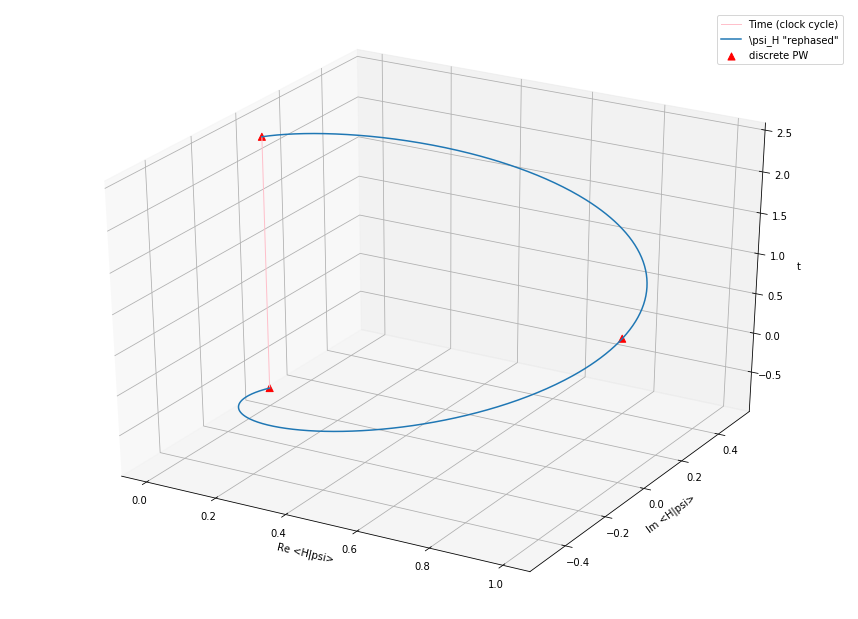
\includegraphics[width=\textwidth]{img/psi_H.png}
  \caption{
    Evolution of $\braket{H}{\psi(t)}$ in the two models.
  }
  \label{fig:psi_H}
\end{figure}

\begin{figure}
  %\centering
  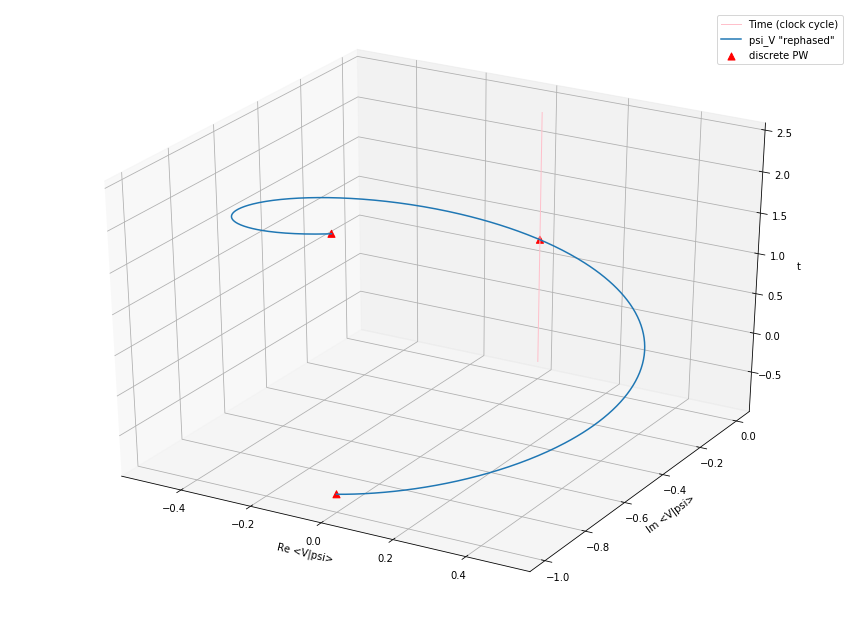
\includegraphics[width=\textwidth]{img/psi_V.png}
  \caption{Evolution of $\braket{V}{\psi(t)}$ in the two models.}
  \label{fig:psi_V}
\end{figure}
  %% something wrong: we're not in an omega eigenbasis and we've not computed Fourier on omega repr even...
\section{Multi-Level Clock}\label{sec:multiLevelClock}

\subsection{Preliminaries}

A clock that can measure only two times in one cycle of a periodic evolution
is of limited interest ---and limited falsifiability, as it can be easily
interpolated by different models.
The experiment described in
\cite{Moreva:synthetic} and related works attempts at addressing the issue:
\begin{quote}
  To obtain a more interesting clock, we perform the same conditional probability measurement
  introducing varying time delays to the clock photon, implemented through quartz plates of
  variable thickness.
\end{quote}
However, it must be noted that such delay is in fact a classical external parameter.
%
In what follows, instead, our approach to a more interesting clock will be based on simply
increasing the number of levels of the clock, or in other words increasing the
finite dimension of the Hilbert space $\hilb{H}_T$. This is certainly feasible
theoretically, possibly resorting to numerical computation.


\subsection{Eigensystem in the product space and consistency with ordinary quantum \mbox{theory}}
\label{sec:building-the-discrete-pw-clock}
Appendix \ref{appendix:n-level} reports the details of
symbolic and
numeric computation for
an $N=32$-level clock, ``timing'' a qubit subject to the same Hamiltonian
of the experiment we have seen in Sec.~\ref{sec:pw:qubit}.

In this case, for simplicity, we work in
``natural units'' $\hbar = \omega = 1$, where $\omega$ is
the characteristic frequency in the same sense of the
two-level clock experiment described in Section \ref{sec:pw:qubit}.

The clock is built as having a time operator which is diagonal in the
chosen computational basis\footnote{
  Here there is no explicit reference to any particular physical implementation.
}:
\[
  \op{T} \repr \frac{2\pi}{N}
  \begin{pmatrix}
    0           &       &       &       \\
                &1      &       &       \\
                &       &\ddots &       \\
                &       &       &N-1
  \end{pmatrix} \,\text{.}
\]
With this choice, the clock spans the characteristic period of $\Delta T = 2\pi$.

The ``spatial space'' or ``ordinary Hilbert space'' $\hilb{H}_S$
is still 2-dimensional, and the Hamiltonian in it is simply
\[
  \op{H}_S \repr
  i
  \begin{pmatrix}
    0   & 1   \\
    -1  & 0
  \end{pmatrix}
  \, \text{.}
\]

Frequency operator $\op{\Omega}$ is derived, analytically, via Fourier
transformation as seen in \eqref{eq:SI_Fourier:Omega}:
\[
  \op{\Omega} = \frac{N}{2\pi} F^{\dagger}_{N} \op{T} F^{}_{N} \, \text{.}
\]
With a large $N$,
such derivation is extremely laborious. We do not resort to
numeric FFT in this case, but we do benefit of computer-aided, yet exact
symbolic computation.

Once $\op{\Omega}$ is derived though,
the eigenvalues and eigenvectors of
$\op{\mathbb{J}} = \hbar\op{\Omega}\ox\idop_S + \idop_T\ox\op{H}_S$
can only, realistically, be computed with numerical methods.

In order to illustrate interesting examples, not corresponding to the
trivial evolution of an eigenstate of $H_S$,
but to some kind of Rabi oscillation or Larmor precession
\parencite[\ch IV]{Cohen-Tannoudji}, we pick, in \term{Mathematica}'s ordering,
just as an example,
eigenvectors $\dket{\Phi_{40}}$ and $\dket{\Phi_{41}}$ of $\op{\mathbb{J}}$
in $\hilb{H}_T \ox \hilb{H}_T$, corresponding to eigenvalues
$\epsilon_{40} = 12$ and $\epsilon_{41} = 11$.

Each eigenvector encodes a whole possible discrete-time history
of the qubit over a cycle.
% as stated in \eqref{eq:timepicks2} or \eqref{eq:timepicksN}.

So, for example, if components $1$ and $2$ of $\dket{\Phi_{41}}$ correspond to
(the components of)
an initial state of the qubit in $\hilb{H}_S$
(i.e at ``ordinary time'' $t=0$); components
$2k + 1$ and $2k + 2$ correspond to $t = \frac{2\pi}{N}k \eqbydef t_k$
of same, $\forall k \in \qty{0, \dots, N-1}$.

A comparison of Page--Wootters results with ordinary
Schr{\"o}dinger evolution is thus given by the comparisons
\begin{align}
  \dbradket{2k+1}{\Phi_{41}} e^{-i \epsilon_{41} t_k} &\sim \braket{0}{\psi(t_k)}_{\mathrm{S}} \label{eq:comparison0} \\
  \dbradket{2k+2}{\Phi_{41}} e^{-i \epsilon_{41} t_k} &\sim \braket{1}{\psi(t_k)}_{\mathrm{S}} \label{eq:comparison1}
  \,\text{,}
\end{align}
where the phase $e^{-i \epsilon_{41} t_k}$ is motivated in \cite[\it ``The Zero-eigenvalue'']{Lloyd:Time},
and inessential if one is merely interested in determining and comparing probabilities
$\qty|\braket{0,1}{\psi}|^2$. Please note the double angle bracket notation for vectors
and algebraic operations in the product space $\hilb{H}_T \ox \hilb{H}_S$.

\begin{figure}
  \centering
  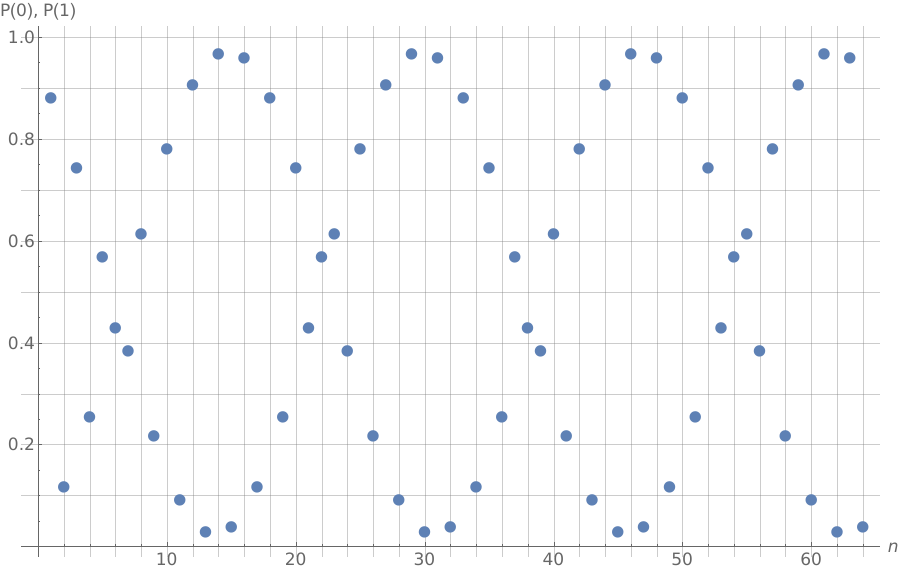
\includegraphics[height=.3\textheight]{img/N32-B.png}
  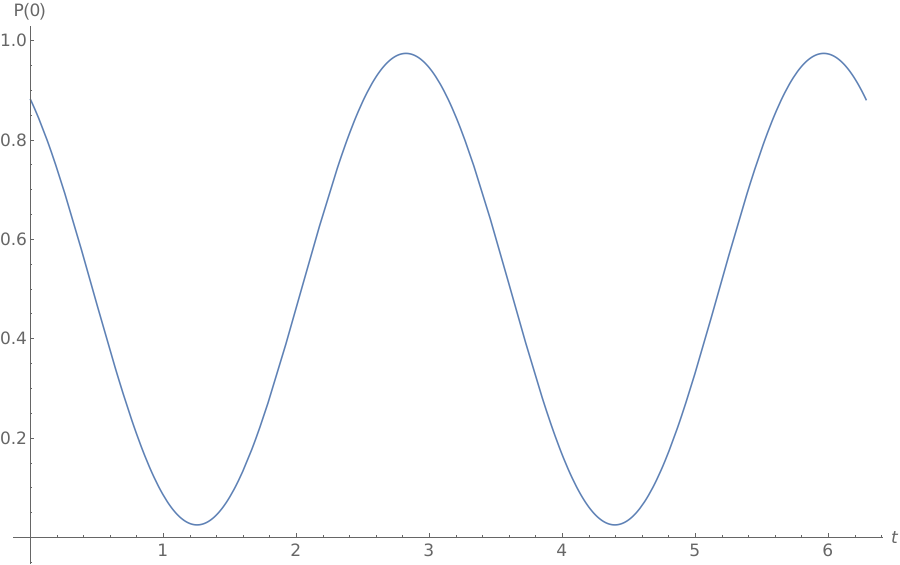
\includegraphics[height=.3\textheight]{img/probB_0.png}
  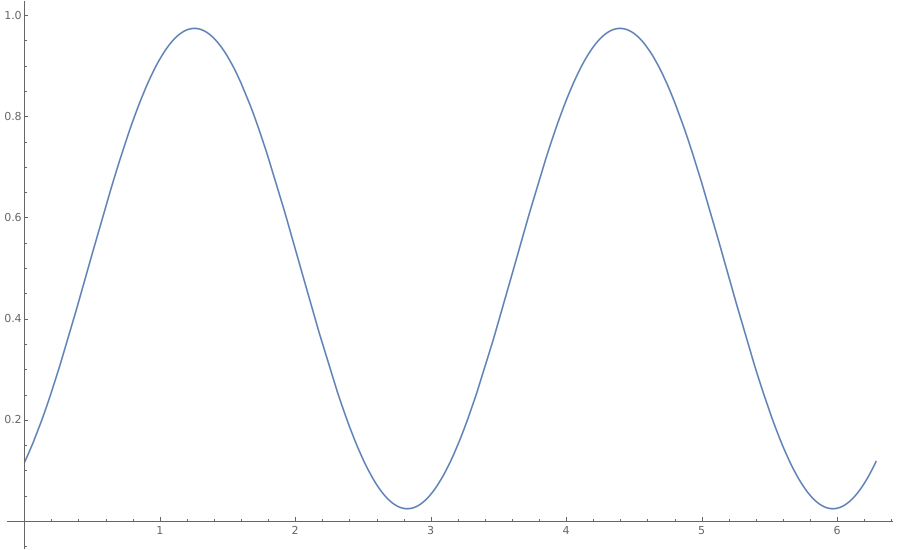
\includegraphics[height=.3\textheight]{img/probB_1.png}
  \caption[
    Page-Wootters vs Schr{\"o}dinger probability evolution
  ]{
    Page-Wootters ({\it top}) vs Schr{\"o}dinger probability evolution. % for $\op{\mathbb{J}}$ eigenvalue $=11$.
    See also Eqs. \eqref{eq:comparison0} and \eqref{eq:comparison0}.
  }
  \label{fig:prob-comparison}
\end{figure}

Figure \ref{fig:prob-comparison} is the graphical representation of (the square modulus of)
\eqref{eq:comparison0} and \eqref{eq:comparison1} i.e. the probability for the qubit
in $\hilb{H}_S$ to be $\ket{0}$ or $\ket{1}$.

The discrete graph, on top, plots the
square modulus of components of $\op{\mathbb{J}}$'s eigenvector $\dket{\Psi_{41}}$.

Odd-index ($2k+1$) square-modulus components
---occupying vertical \emph{spaces} on the grid---
are compared
with the Schr{\"o}dinger evolution of probability $\qty|\braket{0}{\psi}|^{2}$
(first continuous plot, middle image).

Even-index ($2k+2$) components
---occupying vertical \emph{lines} on the grid---
are analogously compared
with the Schr{\"o}dinger evolution of probability $\qty|\braket{1}{\psi}|^{2}$
(second continuous plot, bottom image).

\begin{figure}
  \centering
  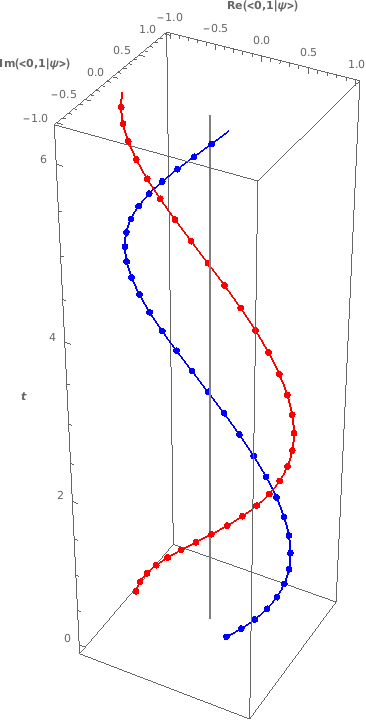
\includegraphics[width=0.45\textwidth]{img/PWfit32.png}
  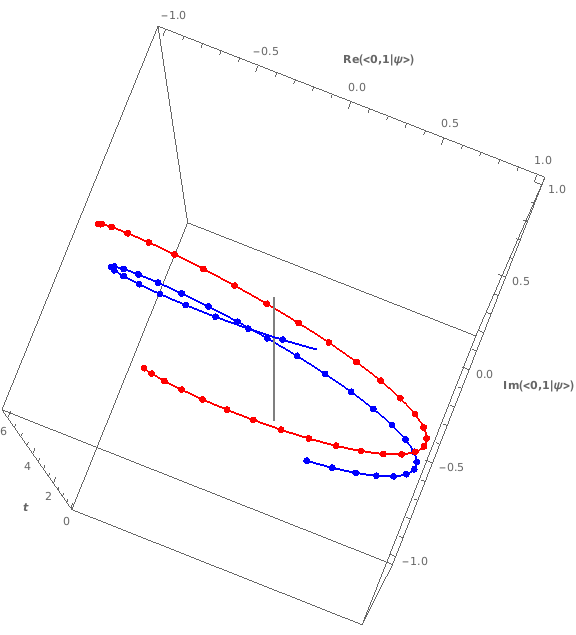
\includegraphics[width=0.5\textwidth]{img/PWfit32top.png}
  \caption[
    P-W vs Schr{\"o}dinger evolution (complex values)
  ]{
    Page--Wootters discrete-time ``evolution without evolution'' (points)
    is interpolated by the (continuous lines) of standard quantum mechanics
    evolution.
    Horizontal axis are real and imaginary part of the wave function components.
    Vertical axis is time $t$.
    Red   line plots {\color{red}   $\braket{0}{\psi(t)}$}.
    Blue  line plots {\color{blue}  $\braket{1}{\psi(t)}$}.
  }
  \label{fig:complex-comparison}
\end{figure}

Finally, Figure \ref{fig:complex-comparison} compares the two sides of
\eqref{eq:comparison0} and \eqref{eq:comparison1}
in terms of \emph{complex value}
(%
  therefore the term $e^{-i \epsilon t_k}$ is relevant,
  for eigenvalues $\epsilon \neq 0$ of $\op{\mathbb{J}}$%
).

\section{Page--Wootters and detector models for a two-level system}

\subsection{Detector models}

As we have seen in the previous sections,
proper elements of $\pwspace$,
localized in both space and time,
can be interpreted as ``events''
(as opposed to full history vectors, which instead describe the unitary evolution
of a quantum system \emph{at all times}).

The arrival of a particle at a detector
is a kind of event
of particular interest from the perspective of time
in quantum mechanics, for several reasons.

The first reason
is the direct connection with experiments,
``given the appalling evidence that time is also a random variable in the laboratories''
\parencite[\ch 4]{TQM2};
and because,
``{[as]} a matter of fact, a number of time observables are already routinely measured in laboratories,
for example arrival times in time-of-flight experiments,
but the theoretical foundation of these measurements is still being discussed''
\parencite[Preface to the First Ed.]{TQM1}.

The second reason is the existence of studies
about detector models which also investigate
time-of-arrival as a quantum observable,
as we have seen in Section \ref{sec:hist:detect}.
None of those works are explicitly
based on Page--Wootters relational model ---of which, to our knowledge,
there are no working examples of application to
time-of-detection problems in the current literature.
Section \ref{sec:absorption+pw} and the remainder of the chapter
will be devoted to bridging such gap
by implementing such application
and comparing
the results from the different models.
Some emphasis will be given to
\emph{discrete} relational time
using the techniques developed in Section \ref{sec:pw:qubit}.

One of the goals of this chapter
is indeed combining PW and detector models.

Another route is POVM, see Chap. \ref{ch:decohere} and \ref{ch:hist}.
Nonetheless, we know that a projective measurement on a bipartite system
can be regarded as a POVM
if we look at
on one part only (e.g. \cite{Paris2012}),
thus the clock space of the Page--Wootters mechanism, $\hilb{H}_T$,
can be regarded as a purification space \parencite{Paris2012} for the ``standard''
Hilbert space where the time-of-arrival POVM is defined,
and an interesting line of further research would be a more formal
study of the logical connection between the two approaches, based on this principle.
Both models respond to the issues raised by Pauli
by giving up
the pursuit of
a \emph{projective} measurement in the \emph{standard} Hilbert space,
and rather ``opening'' that Hilbert space in some sense.


\subsection{Comparison with the Page and Wootters formalism}
\label{sec:absorption+pw}

The detector absorption model in \cite{RuschhauptAbsorption} is not originally
based on the notion of quantum relational time. It is ``ordinary quantum mechanics''
in the sense that states are in $\hilb{H}_S$ with an external parameter time;
but, contrary to quantum mechanics, the potential can be \emph{complex},
causing the norm of the state vector to not be conserved (in fact, vanishing with time).
In other terms, the evolution is not unitary, even for a pure state.
Specifically, the Hamiltonian is corrected by an anti-hermitian term
that models the detector.

One may wonder whether a proper, normalized Page--Wootters ``position-time wavepacket''
(as described in Section \ref{sec:properpw})
can be used to describe \emph{the event of being detected} (or being absorbed).
It's expected to be peaked around the time when the absorption by the detector is maximum.

\citereset
In the detector model of \cite{RuschhauptAbsorption}, the detection
by absorption
corresponds to the \emph{decrease} in norm of the wavefunction.

Therefore we expect the following relation to be true:
\begin{equation}\label{eq:pwkiukas}
  \braket{\phi(t)} = -\dv{t}\norm{\psi_{\text{Kiukas}}(t)}^2 \text{,}
\end{equation}
both sides of which indicate probability of arrival at time $t$.
Here the function $\phi$ of time $t$ has to be intended in the sense of
\eqref{eq:pwphi}.

\citereset
Interestingly, the same paper provides a solution of \eqref{eq:pwkiukas}.
Despite not being based on the Page--Wootters model, eq. 9 in \cite{RuschhauptAbsorption}
equates the squared norm of a ``time representation'' wavefunction
to the opposite derivative of the squared norm of the ``absorbed wavefunction''.
It reads:
\begin{quote}
  We will associate with any wave function $\psi \in \hilb{H}$
  another wave function $\op{\psi}$,
  which is a function of time, so that
  $\abs{\op{\psi}(t)}^2$
  is the arrival probability density. In other words,
  $\op{\psi}$ is a wave function in a time representation. For each
  $t$, $\op{\psi}(t)$ lies in the original Hilbert space $H$.
\end{quote}
Therefore we ``translate''
$$\op{\psi}(t) \text{ into } \ket{\phi(t)}_S$$
and, consequently,
$$\abs{\op{\psi}(t)}^2 \text{ into } \braket{\phi(t)} \text{,}$$
in the language of the Page--Wootters model and within the notation
adopted.

\citereset
Using eq. 8 in \cite{RuschhauptAbsorption} and translating into our notation we have:
\begin{equation}\label{eq:phi_psi_kiukas}
  \op{\psi}(t) \eqbydef
  \ket{\phi(t)}_S =
  \begin{cases}
    \sqrt{\frac{2}{\hbar}} \op{D}^{1/2} \ket{\psi_{\text{Kiukas}}(t)}_S &\text{ if } t > 0 \\
    0 &\text{ otherwise. }
  \end{cases}
\end{equation}
Where at $t \le 0$ the interaction with the detector is yet to come,
but so it is, as a limit, for small values of $t>0$,
in other terms
$\lim_{t \to 0^{+}} \norm{\op{D} \ket{\psi_{\text{Kiukas}}(t)}} = 0$, thus avoiding the apparent discontinuity.

The corresponding Page--Wootters (proper) vector of $\pwspace$ is
\begin{equation}\label{eq:hatpsi:pw}
  \dket{\Phi} = \int \dd{t} \ket{t} \ox \op{\psi}(t) \,\text{,}
\end{equation}
to which the considerations of Section \ref{sec:for-normalized-elements}
and Section \ref{sec:for-normalized-elements} in terms of time--frequency
(or time--energy) uncertainty relation apply, with some analogy
to what \cite{RuschhauptAbsorption} does within its own framework
in relation to $\op{\psi}$ and its Fourier transform.

In that regard, the \eqref{eq:hatpsi:pw} can be reformulated
\begin{equation}
  \dket{\Phi} = \int \dd{\omega} \ket{\omega} \ox \mathcal{F} \op{\psi} (\omega) \,\text{,}
\end{equation}
where it is
\begin{equation}
  \mathcal{F} \op{\psi} (\omega) = - \frac{\sqrt[4]{2} i}{\sqrt{\pi} \left(- \omega^{2} + \sqrt{2} i \omega + 1\right)} \ket{1}
\end{equation}
---see notebook up to Eq.~\eqref{eq:fhatpsi1_omega} for details.


\citereset
\subsubsection{
  (Non-unitary) evolution without evolution:
  plugging the complex potential in the \emph{discrete} Page--Wootters model
}

Similarly to what seen in Section \ref{sec:building-the-discrete-pw-clock}, we build
the clock by defining ---and representing in a convenient basis---
the time operator and the corresponding frequency operator:
\begin{align}
  \op{T} \repr \frac{2\pi}{N}
  \begin{pmatrix}
    0           &       &       &       \\
                &1      &       &       \\
                &       &\ddots &       \\
                &       &       &N-1
  \end{pmatrix}
  &&
  \op{\Omega} = \frac{N}{2\pi} F^{\dagger}_{N} \op{T} F^{}_{N} \, \text{,}
\end{align}
where $F$ is, again, the discrete Fourier operator of order $N$.

Next we define the Wheeler--DeWitt operator $\mathbb{J}$ as in
\eqref{eq:pwHamiltonian}, but $\op{H}_S$ is replaced by the non-hermitian
Hamiltonian of the detector model
$\mathit{K}_S = \op{H}_S - \iu \op{D}_S$
\parencite{RuschhauptAbsorption},
where the subscript $_S$ has been added to stress
that they would act on the $\hilb{H}_S$ part
of the Page--Wootters' $\pwspace$ ``spacetime'':
\begin{equation}\label{eq:pwHamiltonian:nonUnitary}
  \mathbb{J} = \hbar\op{\Omega}\ox\idop_S + \idop_T\ox\qty(\op{H}_S -\iu \op{D}_S) \,\text{.}
\end{equation}
$\op{H}_S$ and $\op{D}_S$ are the same as $\op{H}$ and $\op{D}$
respectively from the \eqref{eq:complexpot}.

We then compute eigenvalues and eigenvectors of $\mathbb{J}$.
Eigenvectors associated to the eigenvalue $0$ will include
the history of the qubit over a ``period''
(of what would have been a periodic evolution, without the absorptive detector).

Eigenvectors associated to non-zero eigenvalues will need a ``phase correction'',
or energy shift\footnote{ Again, see also ref. \cite[\it ``The Zero-eigenvalue'']{Lloyd:Time}. }
as seen, for example, in \eqref{eq:comparison0} and \eqref{eq:comparison1}.
%% TODO? Examiners wanted more clarity ("proof"?). No time right now, and it is not referred anywhere.
%% So just rely on \cite[\it ``The Zero-eigenvalue'']{Lloyd:Time},
%% \eqref{eq:comparison0} and \eqref{eq:comparison1}.
%%
% Or, in a more compact form:
% \begin{equation}
%   \dket{n}_{\text{hist.}} = e^{-\iu \epsilon_n \op{T}} \ox \idop_S \dket{n}
%   \,\text{,}
% \end{equation}
% where $\epsilon_n$'s are eigenvalues of $\mathbb{J}$ and
% $\dket{n}$'s their corresponding eigenvectors.

\citereset
Linear combination of histories $\sum_n \alpha_n \dket{n}_{\text{hist.}}$
are also physically possible\footnote{
  As opposed to (linear combinations of) mere, uncorrected eigenstates of $\mathbb{J}$.
  Indeed, one may observe,
  at least in the case where $\mathbb{J}$ was hermitian,
  that $\setof{\dket{n}}$ is a basis
  of $\pwspace$ therefore
  $\sum_n \alpha_n \dket{n}$ would span \emph{all elements}
  of $\pwspace$ and the theory would not predict anything i.e.
  it would not discriminate unphysical histories.
}
and in fact we pick
one that ensure that the initial state ${}_{T}\bradket{0}{\Psi}$ is equal to $\ket{0}_S$
so to allow a comparison with the example in \cite{RuschhauptAbsorption}.
Such linear combination is not unique. For reasons of numerical stability,
a linear combination with coefficients in the order of 1 would be ideal if it exists.
In this particular problem, it does.
We simply scan, as a first attempt, all possible values ${}_{T}\bradket{0}{n} + {}_{T}\bradket{0}{m}$
to find a combination that is equal to $\ket{0}_S$
-- or maximizes the fidelity with that respect.\footnote{
  See the definition, and invocation, of the function \texttt{find_best()} in Appendix \ref{discrete-page-wootters-model}.
}

All the above numerical computation is implemented with \emph{NumPy} \parencite{comp:numpy},
particularly in appendix
\ref{discrete-page-wootters-model}.
The results are visualized in
Fig. \ref{fig:absorbed-qubit-components_pwlattice},
and are \emph{compatible} with the non-Page--Wootters
solution previously shown in Fig. \ref{fig:absorbed-qubit-components}.

\begin{figure}
  \centering
  \begin{subfigure}[b]{0.49\textwidth}
    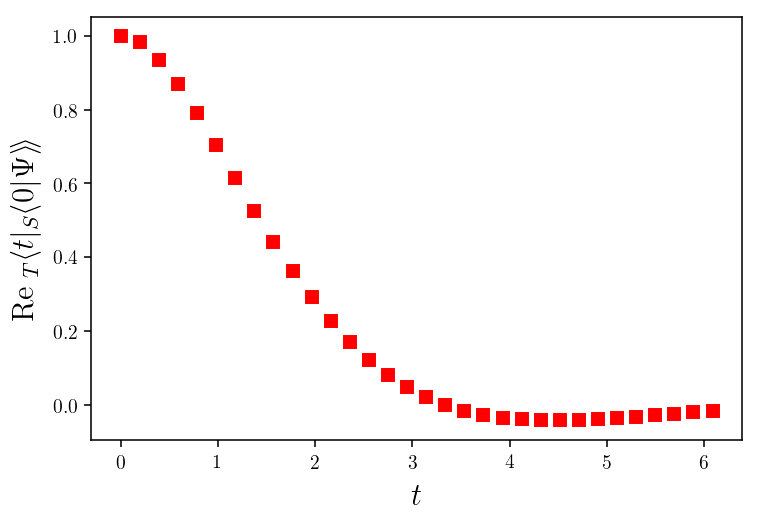
\includegraphics[width=\linewidth]{img/2ldetect/re_psi0_t_pwlattice.png}
    \subcaption{}\label{fig:absorbed-qubit-components_pwlattice:re0}
  \end{subfigure}
  \begin{subfigure}[b]{0.49\textwidth}
    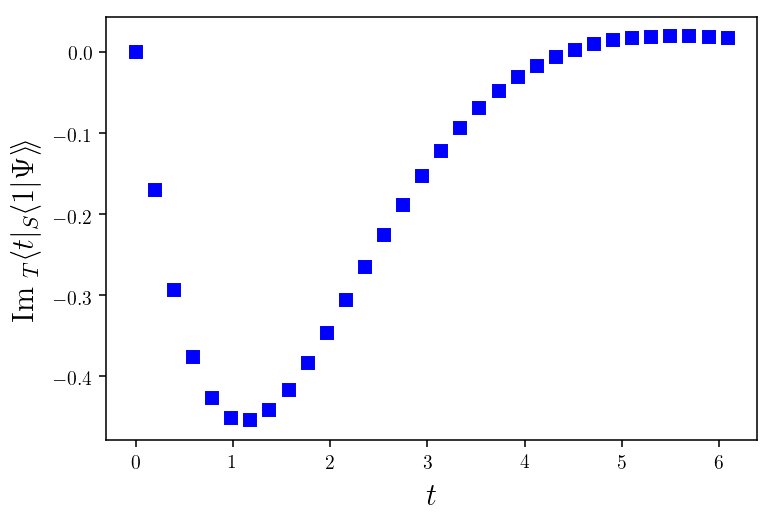
\includegraphics[width=\linewidth]{img/2ldetect/im_psi1_t_pwlattice.png}
    \subcaption{}\label{fig:absorbed-qubit-components_pwlattice:im1}
  \end{subfigure}
  \caption[
    Non-unitary ``evolution without evolution'' (discrete).
  ]{
    Non-unitary ``evolution without evolution''
    using the discrete Page--Wootters model,
    plugging in
    the complex potential of \cite{RuschhauptAbsorption}.
    The result is compatible with the continuous
    ``Schr\"odinger evolution''
    shown in Fig. \ref{fig:absorbed-qubit-components}.
    Note the different notation e.g.
    $\mathrm{Re}{\;}_{T}\hspace{-.2em}\left\langle t | {}_{S}\hspace{-.2em}\left\langle 0 | \Psi \right\rangle\hspace{-.17em}\right\rangle$
    to fit within the framework of the P--W space-time $\pwspace$.
  }
  \label{fig:absorbed-qubit-components_pwlattice}
\end{figure}

\subsubsection{Detection probability amplitude, time of arrival distribution}

In \cite{RuschhauptAbsorption} the probability of detection in time is given
by how fast the norm decreases i.e. $-\dv{\norm{\psi}^2}{t}$.
A ``wavefunction in time'', whose squared modulus equates the detection probability,
is introduced in eq. (8) therein:\footnote{
  Please note we are importing some notation from \cite{RuschhauptAbsorption} as per the symbol $\op{\psi}$,
  at variance to what generally adhered to in this work,
  where the ``hat'' ($\op{\;}$) denotes quantum observables and their corresponding operators.
}
\begin{equation}
  \op{\psi} = \theta(t) \sqrt{2/\hbar}\,\op{D}^{1/2}\,\psi
\end{equation}
In Page--Wootters terms, this translates into applying
$\theta(\op{T}) \ox \sqrt{2/\hbar}\,\op{D}^{1/2}_S$
to the each history vector $\dket{n}_{\text{hist.}}$
(and their linear combinations).
The result is a detection-event \emph{proper} element of ${\pwspace}$
(that would be normalizable in a continuous, infinite-time model too):
\begin{equation}\label{eq:qubit_detection_wavefunction}
  \dket{\Phi_n} =
    \theta(\op{T}) \ox \sqrt{2/\hbar}\,\op{D}^{1/2}_S \dket{n}_{\text{hist.}} =
    \theta(\op{T}) e^{-i\epsilon_{n}\op{T}} \ox \sqrt{2\op{D}} \dket{n} \, \text{.}
\end{equation}
Given we are considering, in our discrete model, only an interval of time within $0$ and $2\pi$,
i.e. all non-negative times (or, more physically, only times when the detector is active),
the Heaviside function $\theta$ (of operator) can be omitted, and simply replaced
by the identity in time $\idop_T$.

Of course, for our problem, we take a linear combination
\begin{equation}
  \dket{\Phi} = \sum_n \alpha_n \dket{\Phi_n}
\end{equation}
where the coefficients $\alpha_n$ are the same that verified
(not necessarily uniquely)
the initial condition of the problem
$\ket{0}_S = {}_T\bradket{0}{\Psi} = \sum_n \alpha_n \, {}_T\bradket{0}{n}_{\text{hist.}} = \sum_n \alpha_n \, {}_T\bradket{0}{n}$.

\citereset
The vector $\dket{\Phi}$, proper element of $\pwspace$,
is the Page--Wootters counterpart of the function
``in time representation'' $\op{\psi}$,
as
described in \cite{RuschhauptAbsorption}. In formulas:
\begin{equation}
  \bradket{t}{\Phi} = \op{\psi}(t) \, \text{.}
\end{equation}

The ``detection wavefunction''~$\dket{\Phi}$ will always lie,
\emph{spatially},
in the space generated by $\ket{1}_S$, or in other terms:
\begin{equation}\label{eq:detect_prob_ampl_only_on_1}
  \prescript{}{T}{\bra{t}}\prescript{}{S}{\bradket{0}{\Phi}} = 0 \text{,} \quad \forall t \, \text{.}
\end{equation}
The linear space of $\ket{1}_S$ is the ``detectable area'' of the qubit
in this problem, and
$\dket{\Phi}$ is essentially the result of the action of the operator $\op{D}$,
that filters non-detectable components out from any vector of $\hilb{H}_S$.

We derive the components of $\dket{\Phi}$ numerically in Section \ref{detection-event},
where they are encoded in the array \texttt{prob_detect_v}.
We observe therein that the \eqref{eq:detect_prob_ampl_only_on_1} is confirmed,
and that ${}_T\!\bra{t} {}_S\!\bradket{1}{\Phi}$ is proportional
to the $\ket{1}$-component of the evolution of the qubit (history $\Dket{\Psi}$)
at any time $t$
(%
  which is not surprising, being $\sqrt{2/\hbar}\op{D}^{1/2}$ of the form
  $\scriptsize \left[\begin{matrix}0 & 0\\0 & \kappa \end{matrix}\right]$%
).
In more formal terms:
\begin{equation}\label{eq:detect_prob_amplitude_proportional}
  \exists \kappa: \: {}_T\!\bra{t} {}_S\!\bradket{1}{\Phi} = \kappa \cdot {}_T\!\bra{t} {}_S\!\bradket{1}{\Psi} \; \forall t \text{,}
\end{equation}
which, algebraically, is almost obvious, given the considerations above.
However, it is worth noting that the expression on the right side
(up to a factor $\kappa$) is, at each $t$,
an ordinary quantum mechanical probability amplitude
(probability amplitude of being $\ket{1}$ rather than $\ket{0}$);
while the expression on the left side, as a function of $t$,
is a probability amplitude \emph{in time}.
Even when normalized (in the probabilistic sense), the two expressions
are proportional but not equal (hence the factor $\kappa$).
This is because the expression on the right must be normalized
so that, at each $t$,
${ \abs{ {}_T\!\bra{t} {}_S\!\bradket{0}{\Psi} }^2 + \abs{ {}_T\!\bra{t} {}_S\!\bradket{1}{\Psi} }^2 = 1 }$
(or, actually, equal to $ \braket{\psi(t)} \leq 1$, the ``lossy norm'' due to absorption).
Whereas the expression on the left must be normalized so that
$\sum_t \norm{ {}_T\!\bradket{t}{\Phi} }_S^2 = P$,
where $P$ is the total probability that the detection/absorption happens at any time,
and it's equal to $1$ for an ideal detection.

\citereset
The probability of detection in time is shown in Fig. \ref{fig:2l_pw_detect_prob_t}
and is \emph{consistent} with the result of
the continuous and not explicitly Page--Wootters model of
\cite{RuschhauptAbsorption} (see Fig. \ref{fig:absorbed-qubit-normalization-loss:t}).

Switching to the frequency (and, therefore, \emph{energy}) domain,
the discrete Fourier transform yields another proper vector
$\Dket{\tilde{\Phi}}$ of $\pwspace$:
\begin{equation}
  \Dket{\tilde{\Phi}} = F \ox \idop_s \dket{\Phi} \, \text{.}
\end{equation}
This vector numerical values, taken pairwise
(or by groups of 3 for a qutrit etc.)
are the components in the computational basis
of the kets $\ket{\tilde{\phi}(\omega)} \in \hilb{H}_S$
such that
\begin{equation}
  \dket{\Phi} = \sum_n \ket{t}\bradket{t}{\Phi} = \sum_{\omega} \ket{\omega}\bradket{\omega}{\Phi}
    = \sum_{\omega} \ket{\omega}_T \ox \ket{\tilde{\phi}(\omega)}_S \, \text{.}
\end{equation}

As a numerical array, $\Dket{\tilde{\Phi}}$ is the representation of $\Dket{\Phi}$
under the basis $\ket{\omega} \ox \ket{0,1}$ instead of $\ket{t} \ox \ket{0,1}$,
where the $\ket{\omega}$ constitute an eigenbasis of angular frequency $\op{\Omega}$.

\citereset
The squared norms $\braket{\tilde{\phi}(\omega)}_{\!S} = \norm{\braDket{\omega}{\Phi}}_S^2$
give the probability of detection in the frequency domain, which is plotted in
Fig. \ref{fig:2l_pw_detect_prob_omega} and, again, consistent
with Fig. \ref{fig:absorbed-qubit-normalization-loss:omega} i.e.
the result from the model of \cite{RuschhauptAbsorption}.

\begin{figure}
  \centering
  \begin{subfigure}[b]{0.49\textwidth}
    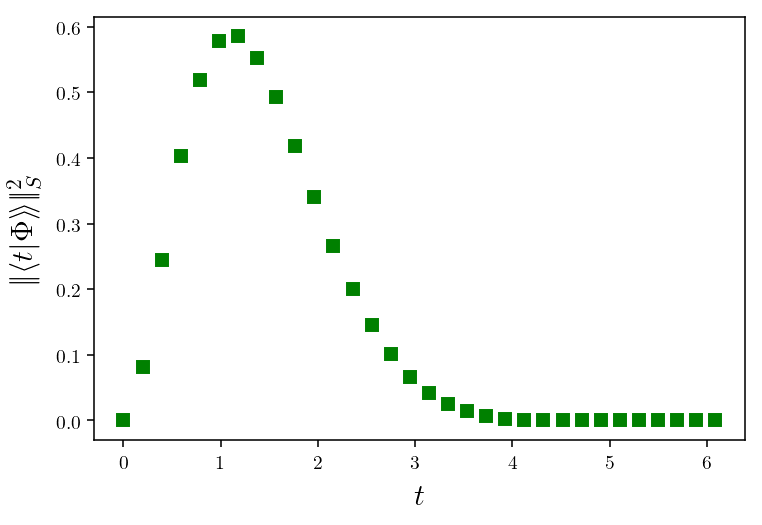
\includegraphics[width=\linewidth]{img/2ldetect/pw-detect-prob.png}
    \subcaption{}\label{fig:2l_pw_detect_prob_t}
  \end{subfigure}
  \begin{subfigure}[b]{0.49\textwidth}
    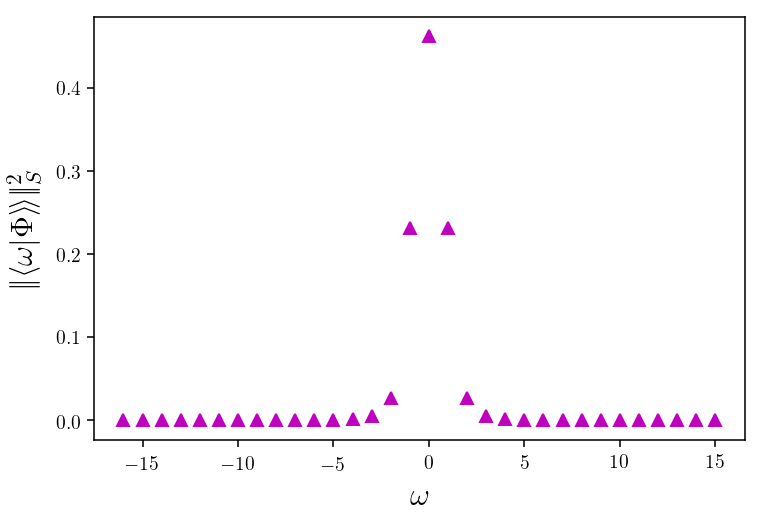
\includegraphics[width=\linewidth]{img/2ldetect/pw-detect-prob-ft.png}
    \subcaption{}\label{fig:2l_pw_detect_prob_omega}
  \end{subfigure}
  \caption[
    Arrival at the detector, probability distribution.
  ]{
    Arrival at the detector, probability distribution:
    \subref{fig:2l_pw_detect_prob_t} in the time domain
    and \subref{fig:2l_pw_detect_prob_omega} in the frequency domain.
  }
  \label{fig:2l_pw_detect_prob}
\end{figure}

\subsubsection{Time--energy uncertainty relation}

% In quantum systems described by a finite Hilbert space,
% uncertainty relations are quantified in terms of \term{entropies}
% of the canonically conjugate probability distributions
% ---see Section \ref{sec:finite_uncertainty} and references therein,
% in particular \cite{FiniteHilb}.

% In our example, the entropic uncertainty relation explicitly reads:
% \begin{multline}
%  S_T + S_{\Omega} =
%   -\sum_t \norm{\bradket{t}{\Phi}}_S^2 \ln \norm{\bradket{t}{\Phi}}_S^2
%   -\sum_{\omega} \norm{\bradket{\omega}{\Phi}}_S^2 \ln \norm{\bradket{\omega}{\Phi}}_S^2 \\
% %
%   = -\sum_{n=0}^{N-1} \left(\abs{\Phi_{2n}}^2 + \abs{\Phi_{2n+1}}^2\right) \ln \left(\abs{\Phi_{2n}}^2 + \abs{\Phi_{2n+1}}^2\right) \\
%     -\sum_{m=0}^{N-1}
%           \left(\abs{\tilde{\Phi}_{2m}}^2 + \abs{\tilde{\Phi}_{2m+1}}^2\right)
%       \ln \left(\abs{\tilde{\Phi}_{2m}}^2 + \abs{\tilde{\Phi}_{2m+1}}^2\right) \\
% %
%   \geq \ln N
% \end{multline}
% ---where we had computed previously the probability values in parenthesis.

% In Section \ref{jupy:entropic-uncertainties}, we numerically find that
% \begin{equation*}
%   S_{T} + S_{\Omega} \approx 1.14 \cdot \ln N
% \end{equation*}
% i.e. circa $14\%$ more than the theoretical minimal uncertainty.

% In terms of uncertainty relation based on standard deviations,
% which is the standard formulation, particularly for continuous distributions,
% and allows a comparison with \cite{RuschhauptAbsorption},
We compute numerically
\begin{equation}\label{eq:uncertainty-us}
  \sigma_{T} \sigma_{\Omega} \approx 0.716 \, \text{,}
\end{equation} \citereset
while \cite{RuschhauptAbsorption} finds
\begin{equation}\label{eq:uncertainty-them}
  \sigma_{T} \sigma_{\Omega} \approx 0.707 \, \text{.}
\end{equation}

TODO:

\url{https://arxiv.org/pdf/2205.02219.pdf}

It is worth observing that the example in the paper
sets the optimal parameters to minimize the time--energy uncertainty
\emph{within the given constraints} of the particular physical system,
they do not necessarily achieve the theoretical Heisenberg minimum of
$\frac{\hbar}{2}$
(or $0.5$ in our numerical problem where $\hbar$ has been adimendsionalized).
More notably, parameters therein have been chosen so to minimize
an alternative definition of time--energy uncertainty, $\expval{T}\sigma_E$,
deemed more meaningful within the physics of the particular system.

\citereset
Nonetheless, with minimal or not minimal uncertainty states (or ``histories''),
a comparison of such uncertainties between the discrete Page--Wootters model implemented
here and the model in \cite{RuschhauptAbsorption} can be performed:
the difference between the results in \eqref{eq:uncertainty-us}
and \eqref{eq:uncertainty-them} may be large enough to be not simply
due to numerical approximation. A further line of investigation
will involve increasing the resolution (number of levels) of the quantum clock:
if the discrepancy persists, an experimental verification
---like those proposed in the paper itself---
will then be of
particular interest. The issue of discriminating different model of arrival time has
been tackled recently in \cite{Maccone_arrival}.

\section{Page--Wootters and detector models for a three-level system}
\label{sec:pw3l}\label{sec:pw:apps_last}

A two-level system is the simplest non-trivial quantum system and,
as seen in Sec.~\ref{sec:absorption+pw},
it is sufficient to illustrate
models of quantum time of arrival,
such as those based on complex potentials,
as well as relational models.
Therein, numerical examples have been shown, where the two approaches
---discrete Page--Wootters and the ``non Hermitian'' detector models---
lead to
compatible predictions.

A three-level atom (or a three-level quantum system in general) appears
naturally
as
the next computational step;
but far from being merely another exercise
---just at a slightly higher level of complexity
but otherwise showing, essentially, the same physics---
it is in fact the \emph{minimal} system \emph{required}
to realize a broad
phenomenology that includes the
\term{Stimulated Raman adiabatic passage}
---STIRAP \parencite{Ruschhaupt_AtomDiode, NonHermitianShortcutSTIRAP, OptimizedTransferSTIRAP, Ruschhaupt_STA23}
and the
\term{Electromagnetically induced transparency}
---EIT \parencite{EIT_Review}.

Also, it is shown that a three-level atom can model
a more robust and realistic
detector for time-of-arrival measurement, compared to the one implemented
with a two-level atom (as introduced in Sec.~\ref{sec:hist:detect}).
The atom can be ``driven'' by a laser
from the ground state $\ket{0}$ into the excited state $\ket{2}$,
then decay into a metastable state $\ket{1}$ at an intermediate energy
(see the above references, although they might use a slightly different notation).
This prevents the atom from decaying again and altering the ``arrival'' detection.

As usual, we're going to set $\hbar = 1$ in the following numerical computation,
based, once again, on the
\emph{NumPy} framework \parencite{comp:numpy},
within a
\term{Jupyter notebook} \parencite{comp:jupyter}.
Details can be consulted in the Appendix~\ref{detector-model-3-level-system}.
Full source code is available from the repository at ref. \cite{OwnJupyterRepo}.

\subsection{Hermitian evolution}

In our numerical example, the following
Hamiltonian is considered:
\begin{equation}\label{eq:3lev:H}
  H \repr \frac{1}{96} \mqty(
    -2  & 0 & 32  \\
     0  & 2 & 8   \\
    32  & 8 & 3
  )
  \text{,}
\end{equation}
with respect to the fiducial basis $\qty{\ket{0}, \ket{1}, \ket{2}}$.
Let also
the initial state be $\ket{\psi(0)} = \ket{0} \repr \mqty(1 \\ 0 \\ 0)$.

The system will evolve \emph{unitarily}, according to $\ket{\psi(t)} = \E^{-\iu H t} \ket{\psi(0)}$,
which is computed numerically:
\begin{lstlisting}[language=Python]
import numpy as np
from scipy.linalg import expm, norm

H = np.array([
  [-2,     0,      32],
  [0,      2,       8],
  [32,     8,       3]
], np.complex_) / 96

psi_0 = np.array([1, 0, 0], np.complex_)

def U(t):
    return expm(-1j*H*t)

def unitary_psi(t):
    return U(t) @ psi_0
\end{lstlisting}

We're interested in the probability of the system to be in $\ket{0}$, $\ket{1}$, or $\ket{2}$,
which is given by $\abs{\braket{0, 1, 2}{\psi(t)}}^2$:
\begin{lstlisting}[language=Python]
def prob(t):
  probabilities = [0, 0, 0]
  for i in 0, 1, 2:
      probabilities[i] = norm(unitary_psi(t)[i])**2
      return probabilities
\end{lstlisting}
Such probabilities over time are shown in Figure \ref{fig:3lev:probs}. 

\begin{figure}[]
  \begin{subfigure}[b]{\textwidth}
    \centering
    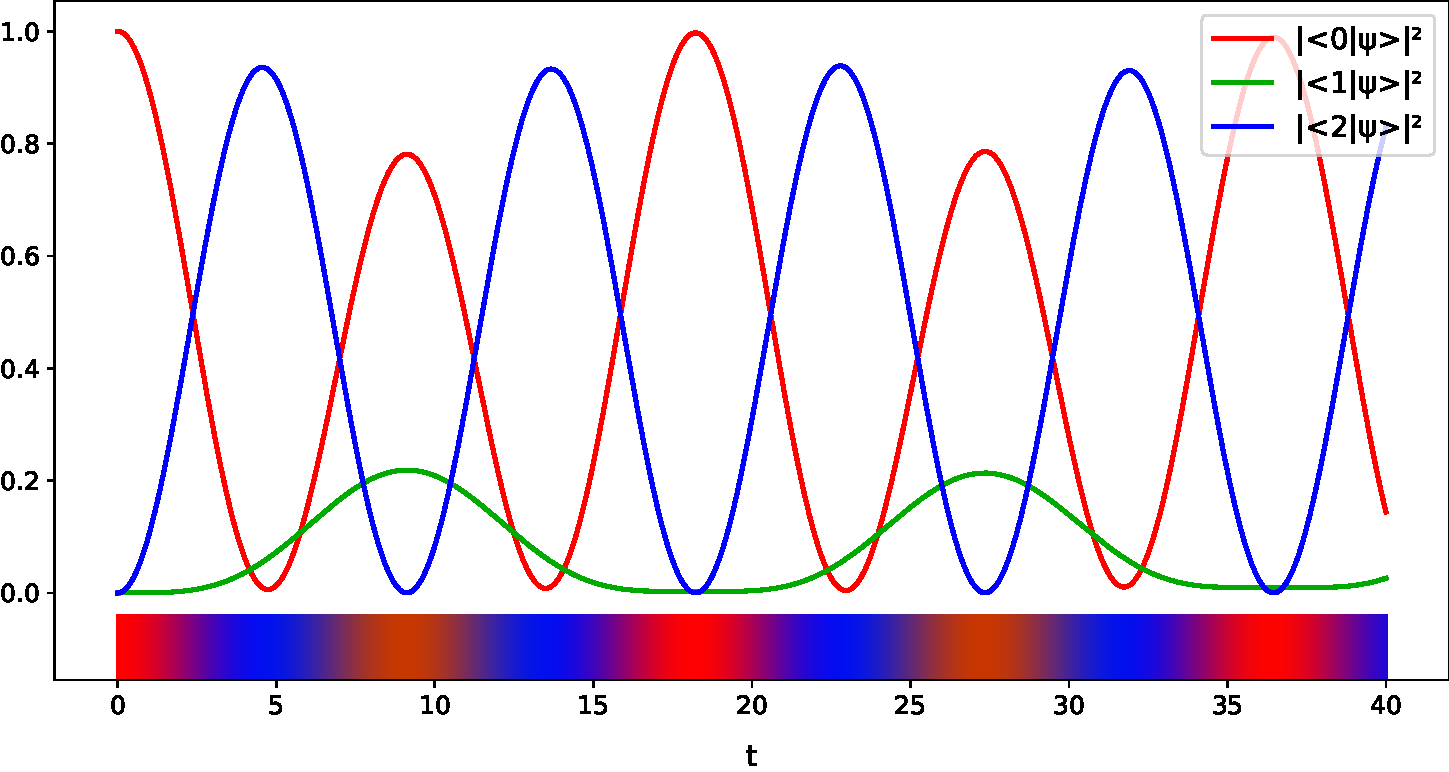
\includegraphics[width=.8\textwidth]{img/3ldetect/hermitian3lines.pdf}
    \subcaption{
      Probabilities for the three-level system.
      \emph{Note}:
        a three-level system allows a graphical representation
        where primary colors can be combined
        (see the bar at the bottom) to immediately
        visualize which probability dominates.
    }
    \label{fig:3lev:probs:lines}
  \end{subfigure}
  \par\bigskip
  \par\bigskip
  \begin{subfigure}[b]{\textwidth}
    \centering
    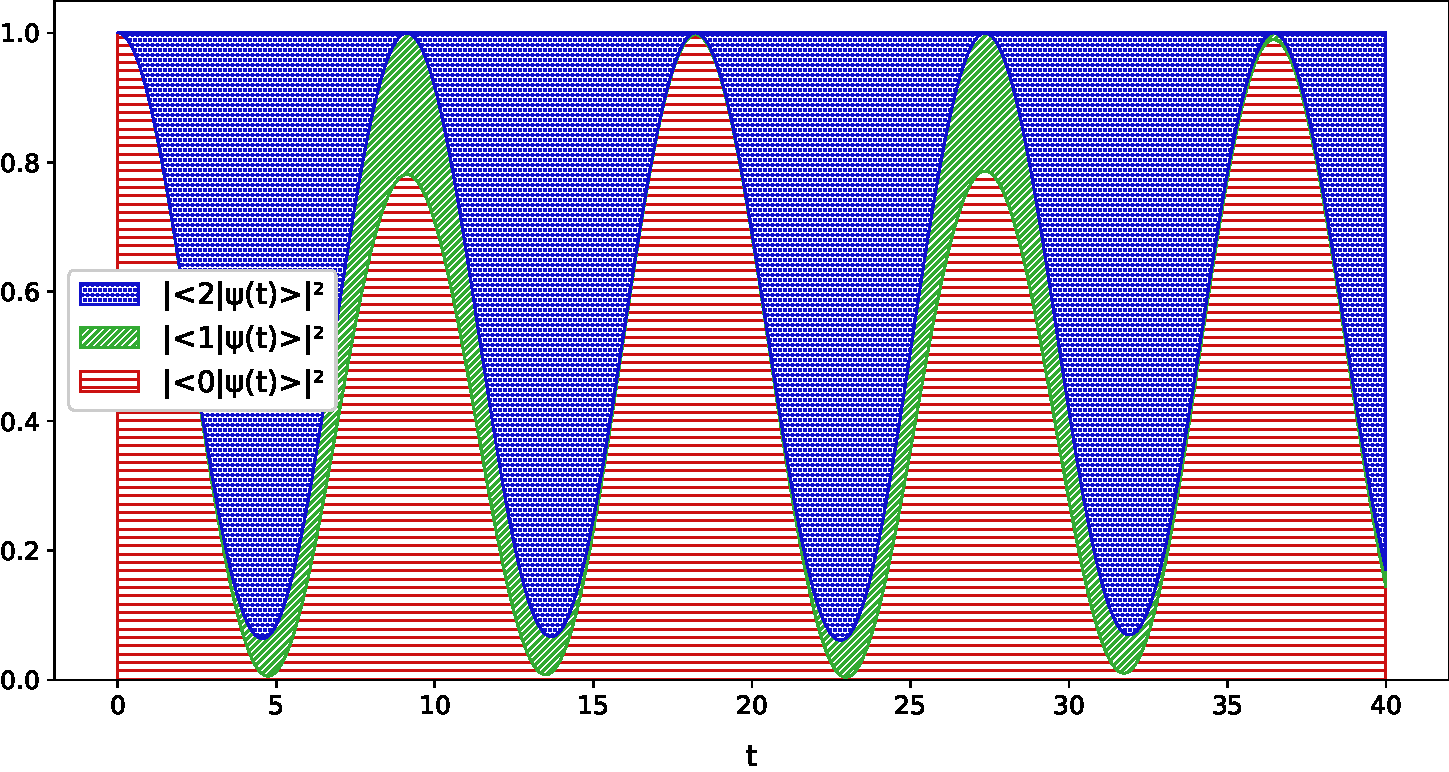
\includegraphics[width=.8\textwidth]{img/3ldetect/hermitian3color.pdf}
    \subcaption{\setstretch{1.25}
      \emph{Stacked} probability chart shows that their sum
      $\sum_{i=0}^{2} \abs{\braket{i}{\psi(t)}}^2$
      is constantly equal to 1 at any time $t$.
      That is equal to the norm $\norm{\psi(t)}^2$, which is indeed conserved
      as
      the system evolves \emph{unitarily}.
    }
    \label{fig:3lev:probs:stack}
  \end{subfigure}
  \par\bigskip
  \par\bigskip
  \caption{
    Probabilities
      $\abs{\braket{i}{\psi(t)}}^2$ for $i \in \qty{0, 1, 2}.$
  }
  \label{fig:3lev:probs}
\end{figure}

We are also interested in probability \term{amplitudes}:
complex values of
$\braket{0}{\psi(t)}$, 
$\braket{1}{\psi(t)}$, and
$\braket{2}{\psi(t)}$
are represented in the three-dimensional
plot in Fig.~\ref{fig:3lev:hermitianEvol}.
Once again, the two horizontal axes are used for the real and imaginary part of
$\braket{0, 1, 2}{\psi(t)}$,
while the independent variable $t$ (time) is represented on the vertical axis.
\begin{figure}[]
  \begin{subfigure}[t]{\textwidth}
    \centering
    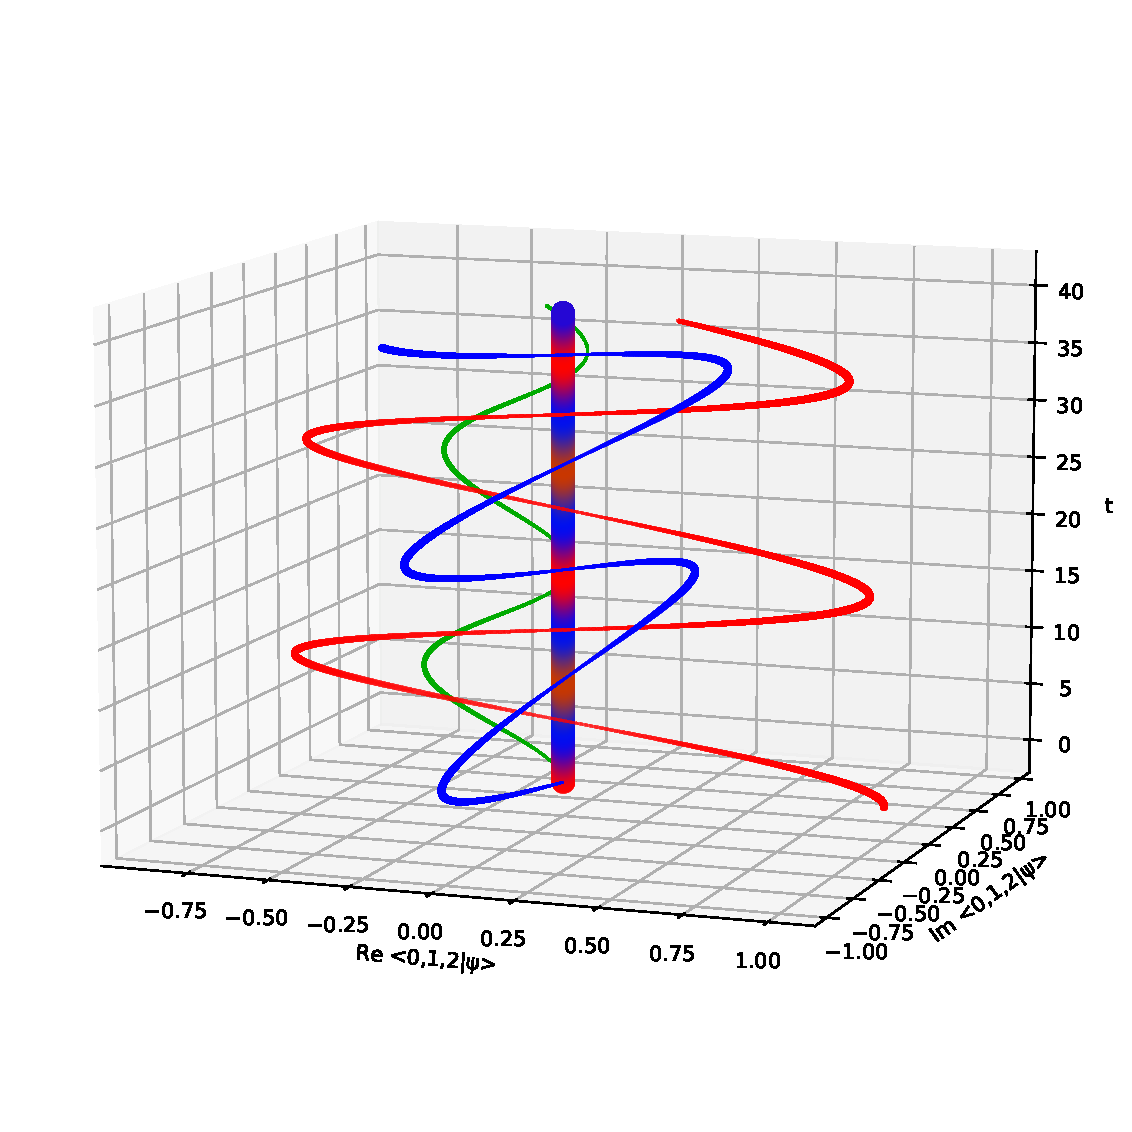
\includegraphics[height=0.45\textheight,clip,trim=80 180 40 140]{img/3ldetect/hermitianSpaceTime_side.pdf}
    \caption{``Side'' view.}
  \end{subfigure}
  \par\bigskip
  \begin{subfigure}[b]{\textwidth}
    \centering
    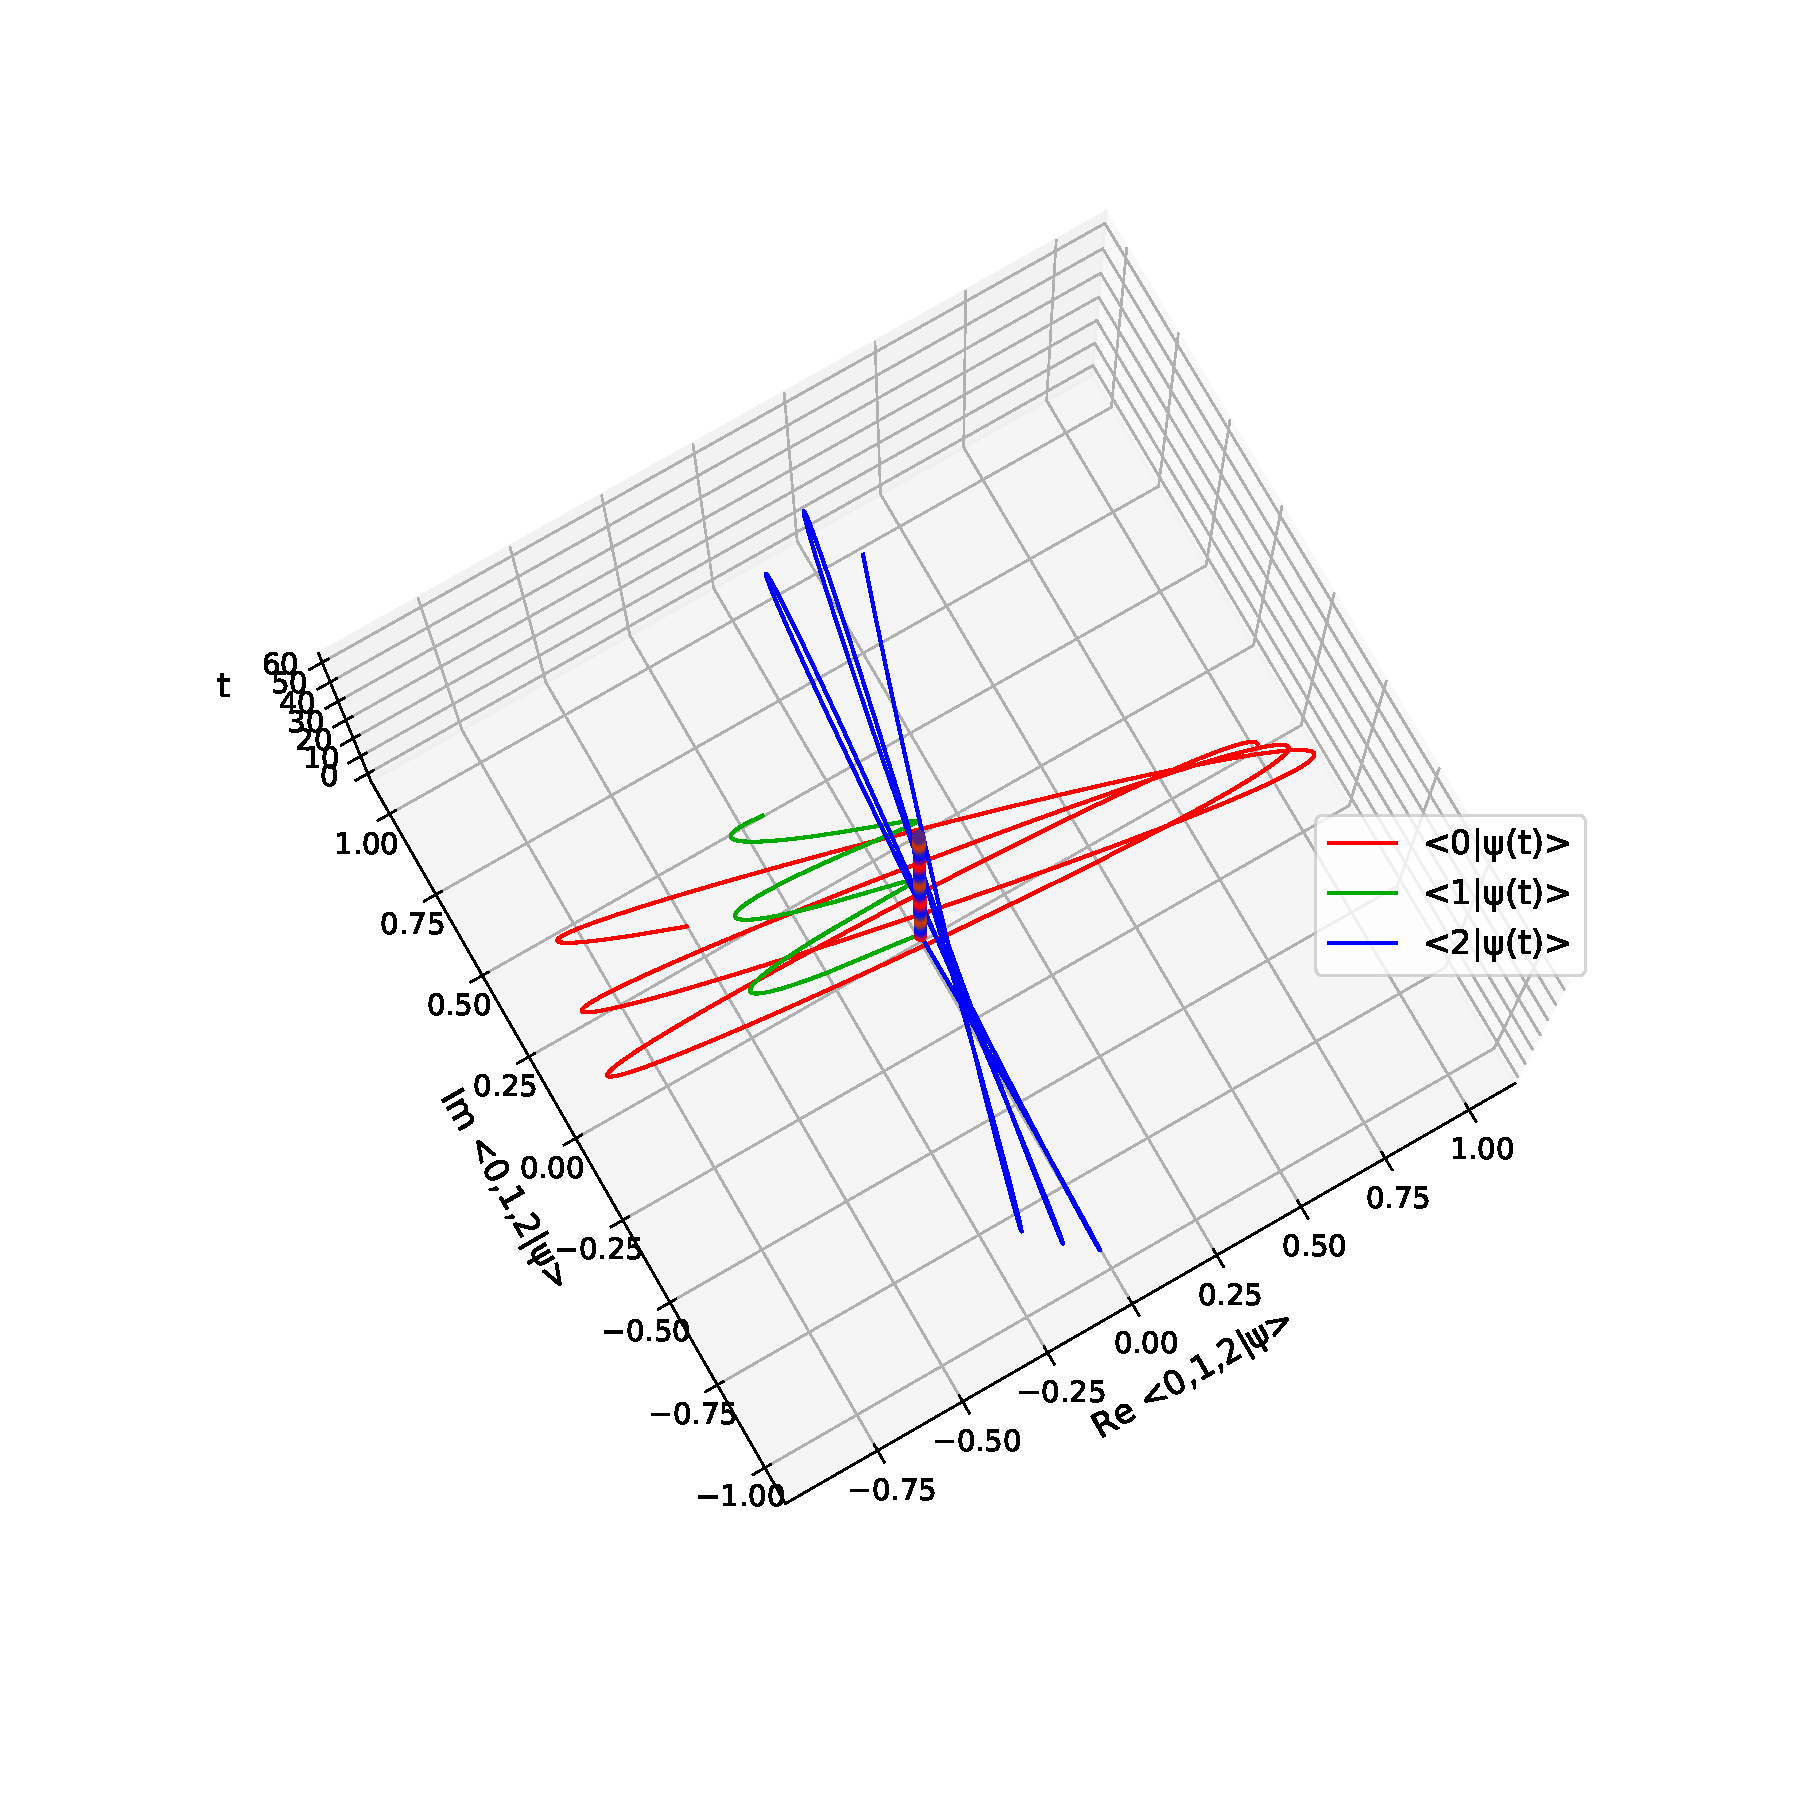
\includegraphics[height=0.41\textheight,clip,trim= 20 120 20 220]{img/3ldetect/hermitianSpaceTime_top.pdf}
    \caption{``Top'' view.}
  \end{subfigure}
  \caption[
    Complex values of the
    probability \emph{amplitudes} $\braket{0, 1, 2}{\psi(t)}$.
  ]{
    \textit{3-D plot} showing the complex values of the
    probability \emph{amplitudes} $\braket{0, 1, 2}{\psi(t)}$.
    Real and imaginary parts of those values are represented on
    the first two axes, while the independent variable (time, $t$)
    is represented
    on the third axis.
    -- Additionally, the vertical axis is coloured to encode \emph{probabilities}
    (absolute values)
    in a similar fashion to Fig. \ref{fig:3lev:probs:lines}. 
  }
  \label{fig:3lev:hermitianEvol}
\end{figure}

\subsection*{\textit{A note on graphical representation}}

Other than visualizing complex-valued functions with three-dimensional plots,
another visualization technique, utilized in various plots in this Section,
consists of leveraging
the fact that the system has exactly 3 levels,
thus allowing three primary colors, red, green and blue, to be combined
in proportion to the probabilities $\abs{\braket{i}{\psi(t)}}$
respectively for $i = 0, 1, 2$. This allows an immediate visualization
of which level, $\ket{0}$, $\ket{2}$ or $\ket{2}$, predominates statistically, if any.
To better clarify this with an example,
a snippet of the implementation of Fig. \ref{fig:3lev:probs} follows.
\begin{lstlisting}[language=Python]
# [...]
import matplotlib
import matplotlib.pyplot as plt

# [...]
for i in 0, 1, 2:
  probs[i] = np.fromiter((prob(t)[i] for t in times), np.float)

# [...]
rgbs = []
for i in range(NPLOTPOINTS):
    rgbs.append(
        (
            probs[0][i],
            probs[1][i],
            probs[2][i]
        )
    )

# [...]
fig, ax = plt.subplots(figsize=(12,6))
ax.set_xlabel('t')
ax.scatter(times, np.zeros(NPLOTPOINTS)-0.1, c=rgbs, marker='|', s=400)
\end{lstlisting}


\subsection{Complex potential -- non-Hermitian evolution}\label{sec:3lev:complexPotential}

In a similar fashion to what seen in Section \ref{sec:hist:detect},
the Hermitian Hamiltonian $\op{H}$, from eq.~\eqref{eq:3lev:H},
is replaced by
\begin{equation}\label{eq:3lev:nonUnitaryH}
  K \eqbydef \op{H} - \iu \op{D} \text{,}
\end{equation}
where
\begin{equation}\label{eq:3lev:nonUnitaryH:antiHermitianTerm}
  \op{D} \repr \mqty(
    0 &0 &0 \\
    0 &0 &0 \\
    0 &0 &\gamma
  ) \text{.}
\end{equation}
This models the absorptive detection of the ``arrival'' of the system at state~$\ket{2}$.
A numeric value of $\gamma = \mathtt{0.1}$ is chosen for the current simulation.
Repeating the calculation for the time-evolution
brings to
probabilities, and probability amplitudes,
that are graphically visualized in Fig. \ref{fig:3lev:loss3color}, and \ref{fig:3lev:nonHermitianEvol},
and can be compared with the Hermitian (i.e. unitary) case,
Figs. \ref{fig:3lev:probs:stack} and \ref{fig:3lev:hermitianEvol} respectively.
It appears clearly, in Fig. \ref{fig:3lev:loss3color},
that the norm of the state vector is not
conserved, but decreases monotonically. 
%
\begin{figure}[]
  \begin{subfigure}[b]{\textwidth}
    \centering
    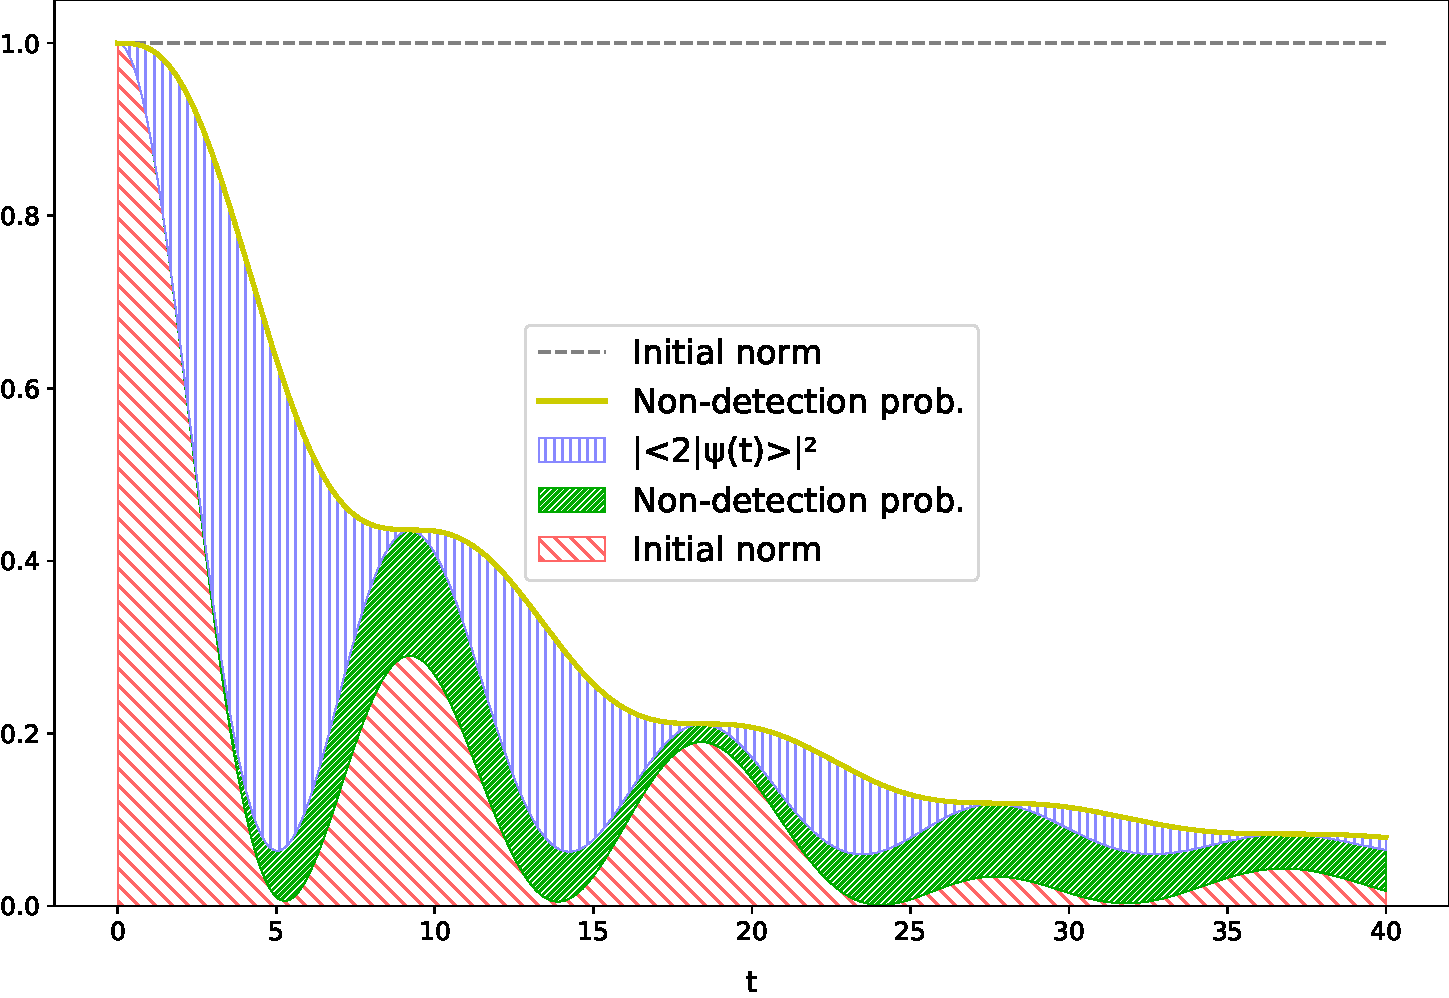
\includegraphics[width=.8\textwidth]{img/3ldetect/loss3color.pdf}
    \subcaption{\setstretch{1.33}
      \emph{Stacked} probability chart (non-Hermitian case) shows that norm
      $\norm{\psi(t)}^2 = \sum_{i=0}^{2} \abs{\braket{i}{\psi(t)}}^2$
      is monotonically decreasing. The actual state probabilities
      will need to be renormalized due to the norm loss of $\ket{\psi(t)}$.
    }
    \label{fig:3lev:loss3color}
  \end{subfigure}
  \par\bigskip
  \par\bigskip
  \begin{subfigure}[b]{\textwidth}
    \centering
    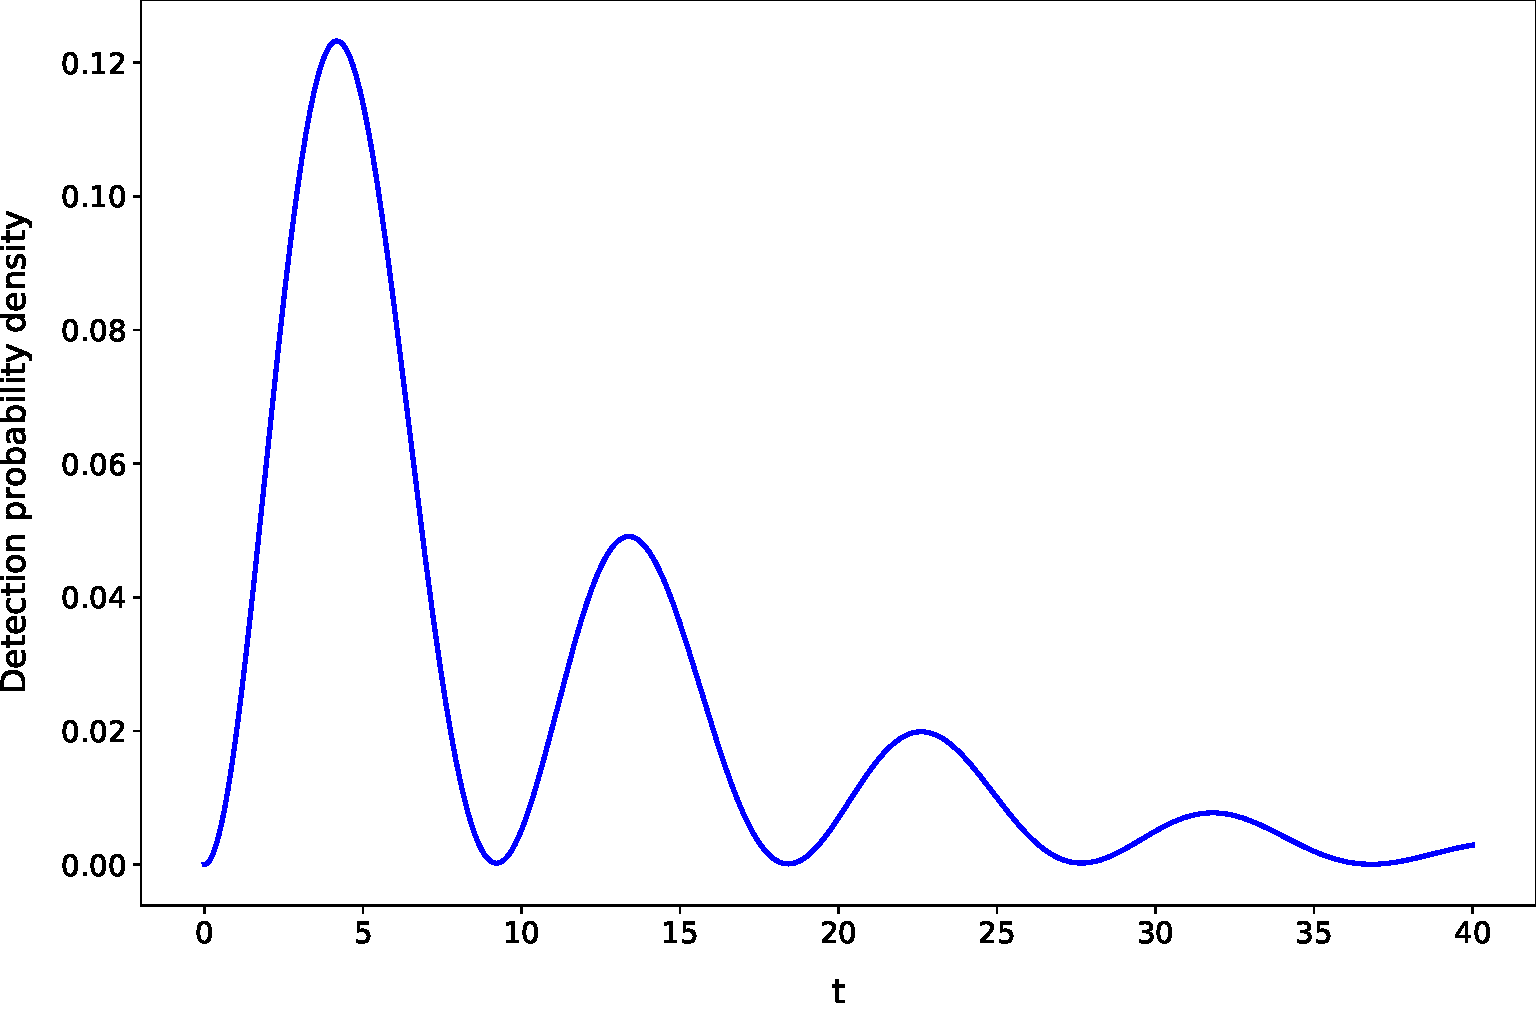
\includegraphics[width=.8\textwidth]{img/3ldetect/loss.pdf}
    \subcaption{
      Normalization loss rate $-\dv{\norm{\psi}^2}{t}$.
      Equates the time-of-arrival probability distribution (at the ``absorbing'' state $\ket{2}$).
    }
    \label{fig:3lev:loss}
  \end{subfigure}
  \par\bigskip
  \par\bigskip
  \caption{
    Absorptive detector model: norm loss and probabilities.
  }
  \label{fig:3lev:nonHermitianProbs}
\end{figure}
%
\begin{figure}[]
  \begin{subfigure}[b]{\textwidth}
    \centering
    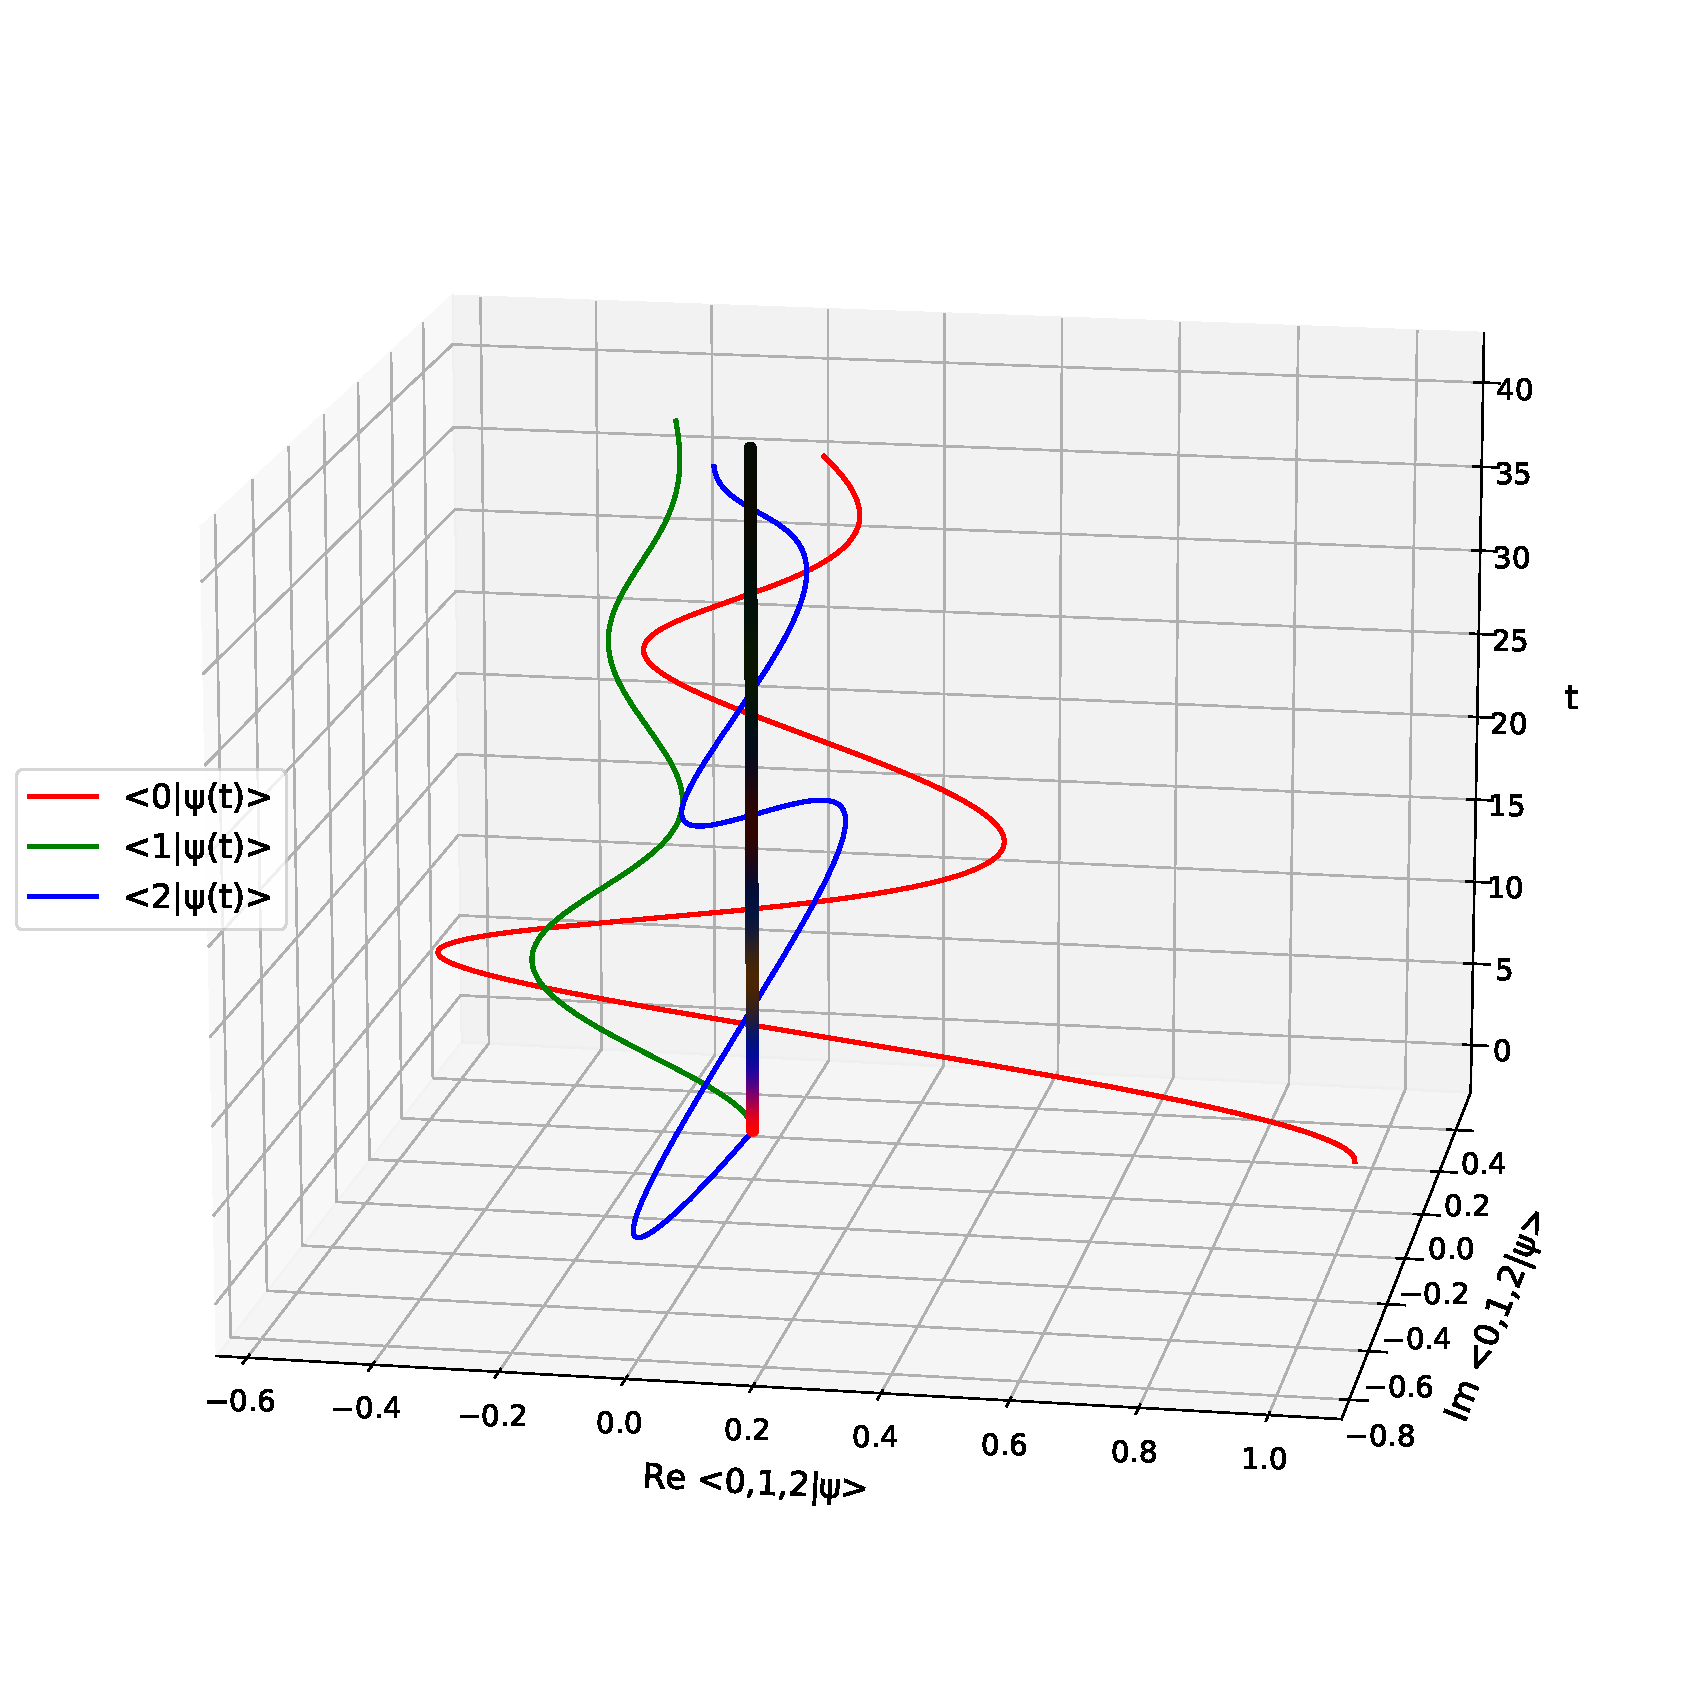
\includegraphics[height=0.41\textheight,clip,trim=0 90 40 140]{img/3ldetect/NonHermitianSpaceTime_side.pdf}
    \caption{``Side'' view.}
  \end{subfigure}
  \par\bigskip
  \begin{subfigure}[b]{\textwidth}
    \centering
    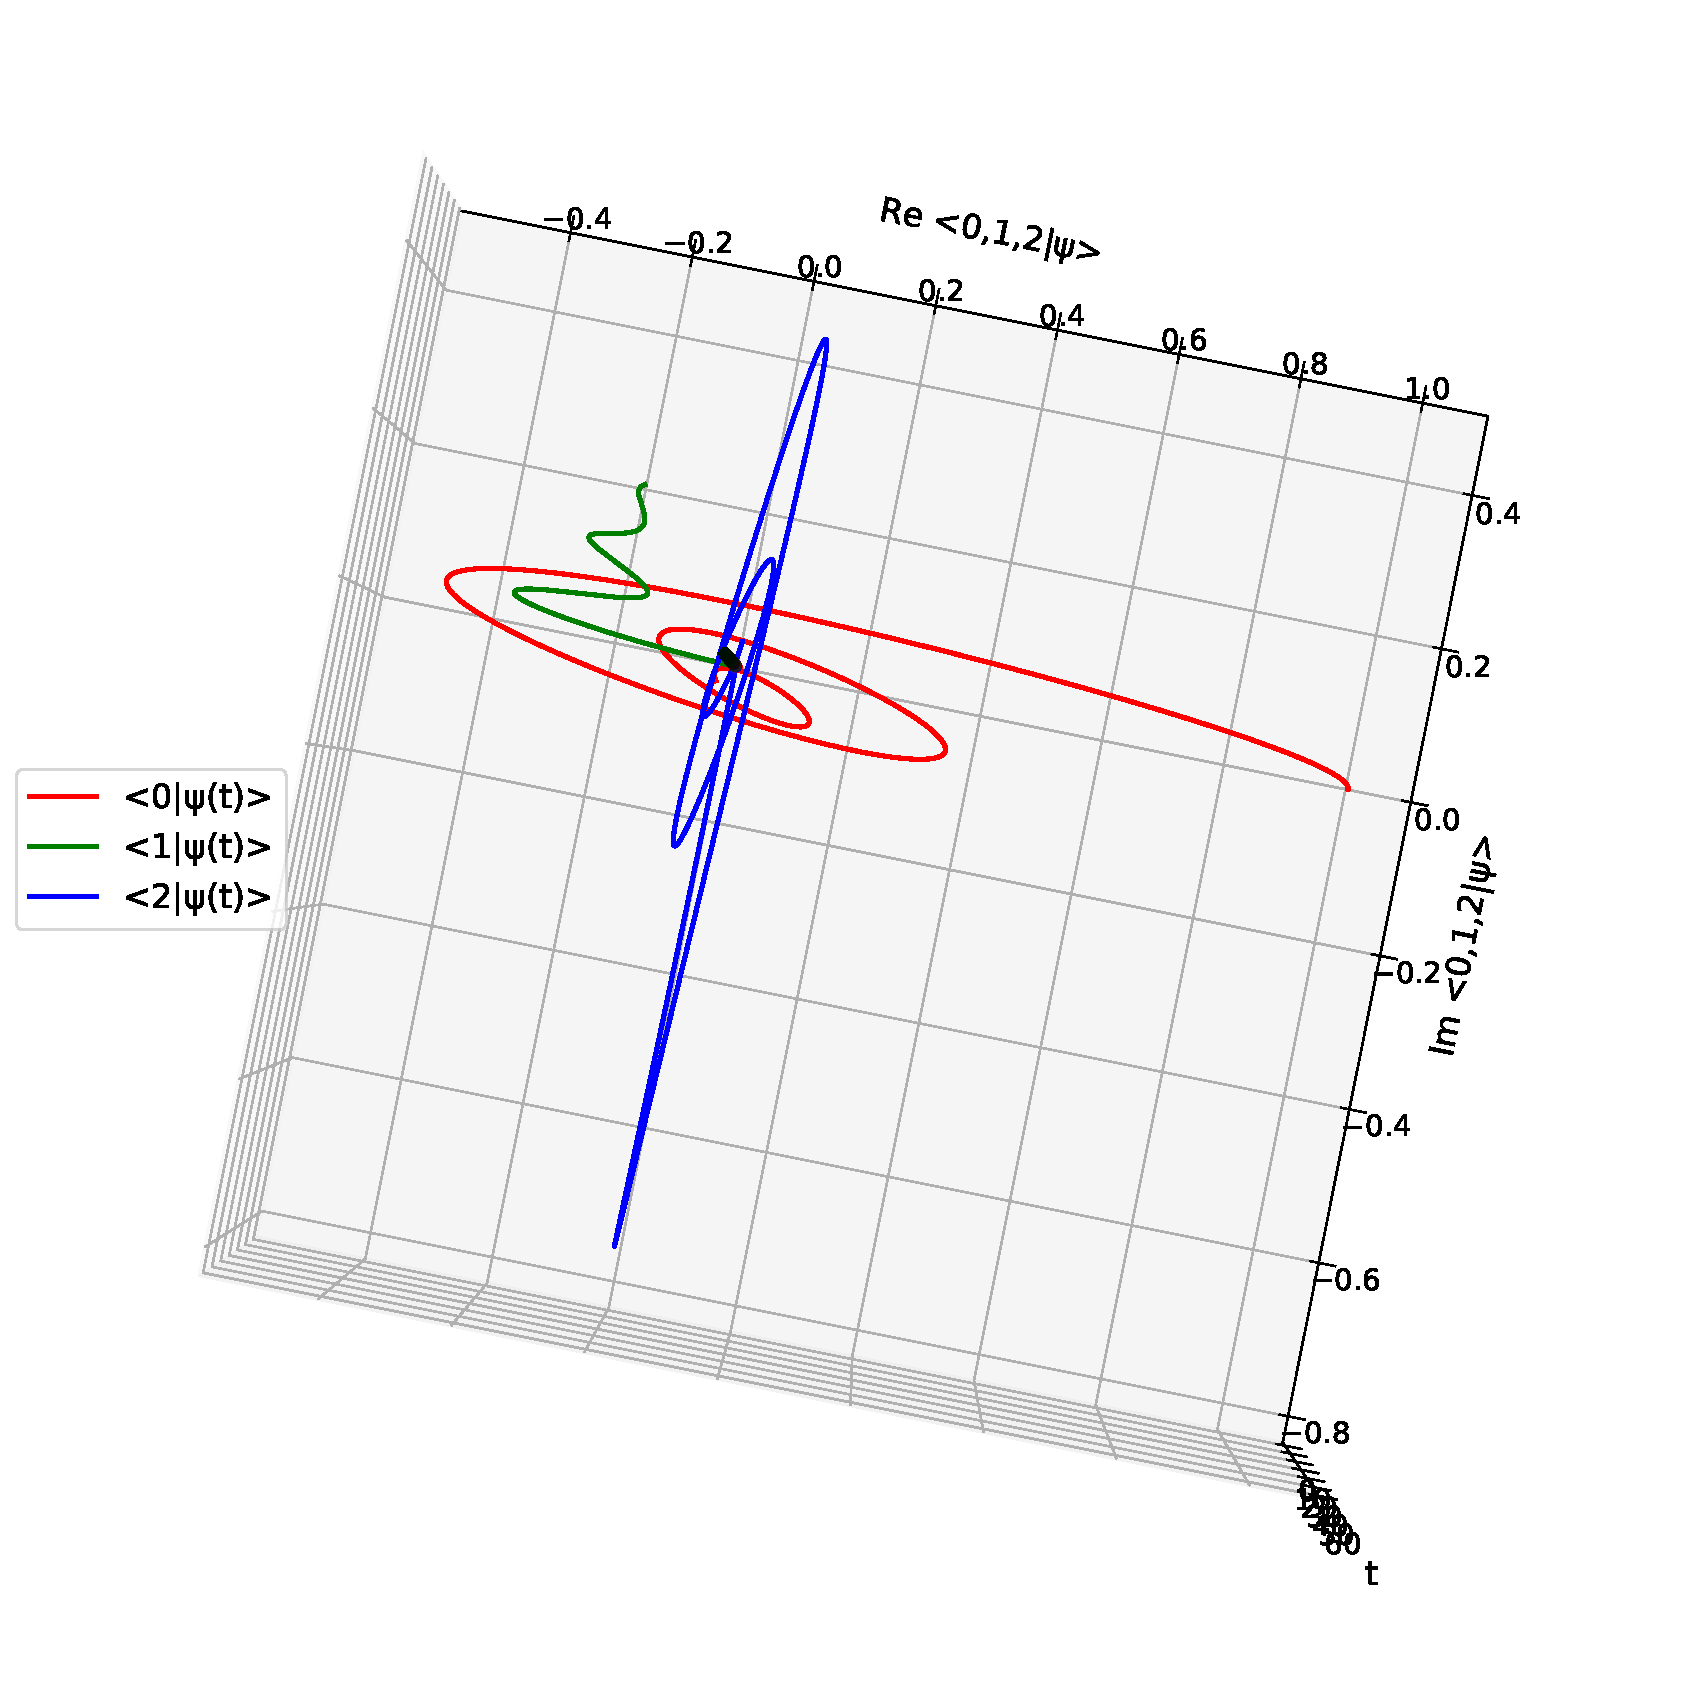
\includegraphics[height=0.44\textheight,clip,trim= 0 90 20 75]{img/3ldetect/NonHermitianSpaceTime_top.pdf}
    \caption{``Top'' view.}
  \end{subfigure}
  \caption[
    Probability amplitudes, with ``lossy'' norm
  ]{
    Non-Hermitian evolution: 3-D complex plot: probability amplitudes, with ``lossy''
    norm (visually, lines get closer to the time axis as $t$ increases).
  }
  \label{fig:3lev:nonHermitianEvol}
\end{figure}

According to the absorptive detector model, the loss of normalization
$-\dv{\norm{\psi}^2}{t}$ indicates the probability of detection
with respect to time, in other words: the time-of-arrival
probability distribution. It is plotted in Fig. \ref{fig:3lev:loss}.

The same results
about probabilities and normalization loss
are plotted
over a longer time interval
in Fig.~\ref{fig:3lev:nonHermitianProbs_ext}.
By comparing the latter,
back with Fig.~\ref{fig:3lev:probs:stack},
it's apparent that in the unitary case the system
periodically oscillates between $\ket{0}$ and $\ket{2}$
---transitioning through the intermediate level $\ket{1}$,
but with a small value of $\abs{\braket{1}{\psi(t)}}^2$.
Instead, within the non-unitary evolution, and with the chosen parameters,
the system is ``driven'' from $\ket{0}$ to $\ket{1}$ and,
after a transient oscillation between the three levels,
shows an asymptotic behavior.
The fidelity with respect to $\ket{1}$,
$\frac{\abs{\braket{1}{\psi(t)}}^2}{\norm{\psi(t)}^2}$,
evaluated numerically at $t=150$ is given by
\begin{lstlisting}[language=Python]
# Pick the last value of time
times_extended[-1]
\end{lstlisting}
\begin{lstlisting}
150.0
\end{lstlisting}
\begin{lstlisting}[language=Python]
# Fidelity
(np.abs(evolution_extended[1])**2)[-1] / norms_extended[-1]**2
\end{lstlisting}
The result is about $94\%$.
\begin{lstlisting}
0.9414855990054901
\end{lstlisting}
It's also worth noting that the norm does not fully vanish with $t \rightarrow +\infty$,
meaning there is a finite probability that detection (or ``absorption'', or spontaneous decay) never happens:
\begin{equation*}
  P_{\mathrm{nd}} = \lim_{t \rightarrow +\infty} 1 - \norm{\psi(t)}^2 \text{.}
\end{equation*}
At the ``large'' value of $t=150$ of our numerical computation, this yields
\begin{lstlisting}[language=Python]
norms_extended[-1]**2
\end{lstlisting}
\begin{lstlisting}
0.05684539507975811
\end{lstlisting}
i.e. roughly 6\% of non-absorption probability.
%
\begin{figure}[]
  \begin{subfigure}[b]{\textwidth}
    \centering
    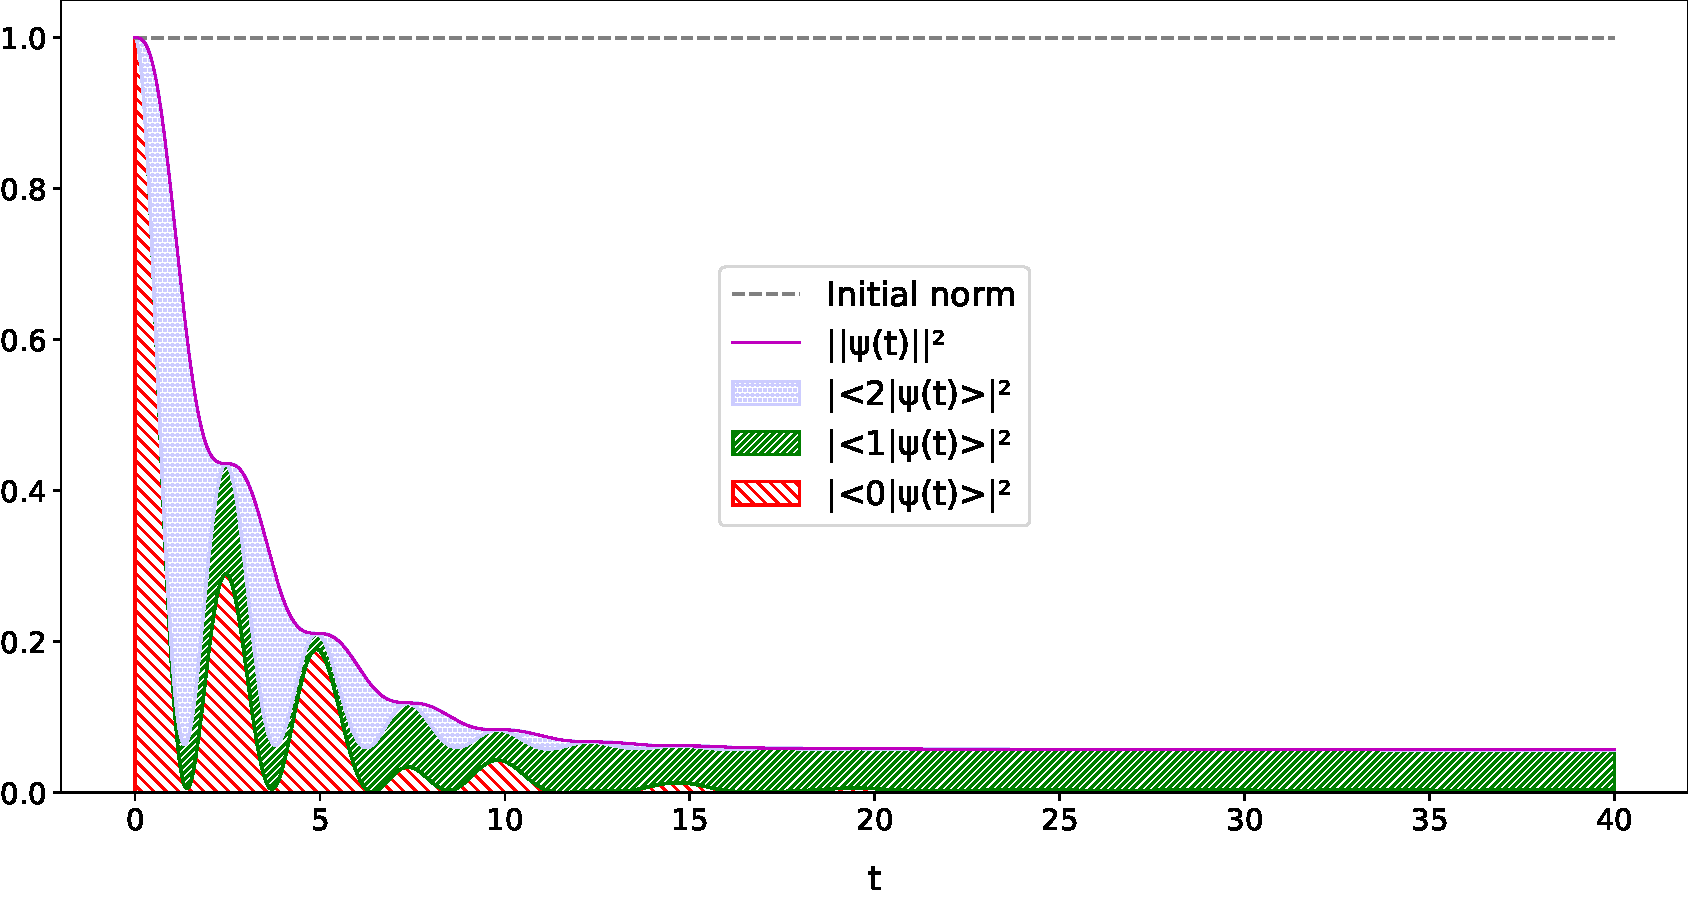
\includegraphics[width=\textwidth]{img/3ldetect/loss3color_ext.pdf}
    \subcaption{
      Probabilities and normalization loss.
    }
    \label{fig:3lev:loss3color_ext}
  \end{subfigure}
  \par\bigskip
  \par\bigskip
  \begin{subfigure}[b]{\textwidth}
    \centering
    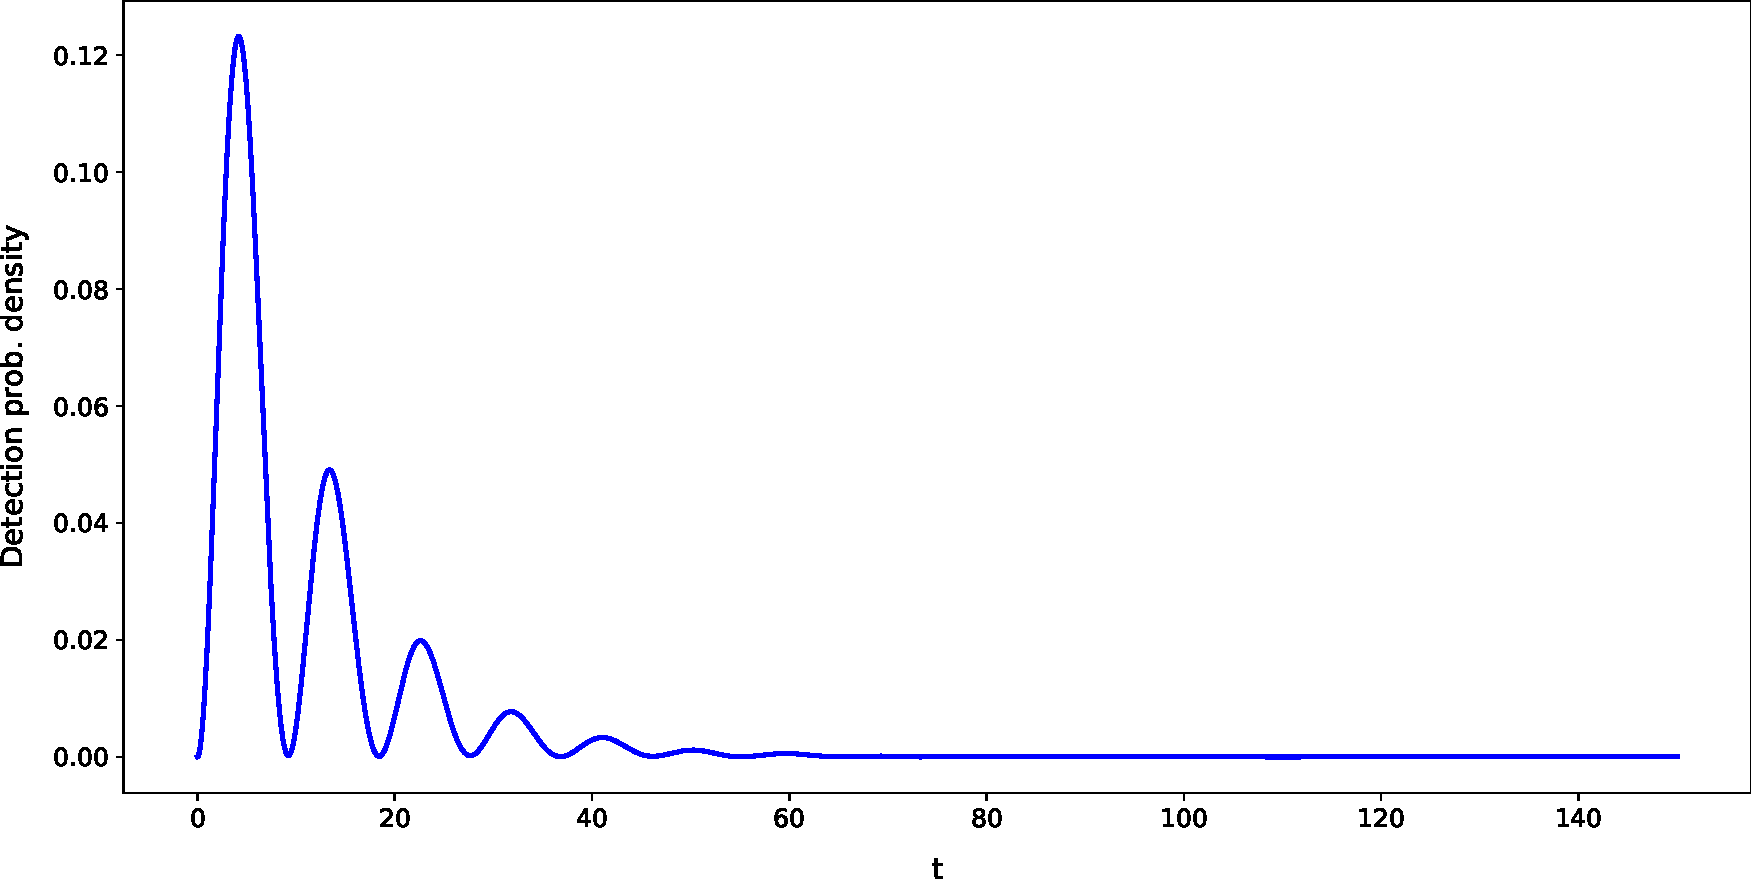
\includegraphics[width=\textwidth]{img/3ldetect/loss_ext.pdf}
    \subcaption{
      Normalization loss rate, or time-of-arrival probability distribution.
    }
    \label{fig:3lev:loss_ext}
  \end{subfigure}
  \par\bigskip
  \par\bigskip
  \caption[
    Absorptive detector model: evolution over a longer time interval.
  ]{
    Absorptive detector model: same results as in Fig.~\ref{fig:3lev:nonHermitianProbs},
    over a longer time interval.
  }
  \label{fig:3lev:nonHermitianProbs_ext}
\end{figure}

\subsection{Discrete Page--Wootters}

Let us consider a Page--Wootters \emph{discrete} clock, with $N_{T}$ levels,
i.e. the clock Hilbert space has finite dimension $N_{T}$,
where we choose $N_{T} = 60$
(somehow resembling the 60 ticks indicating minutes or seconds
in a conventional clock\footnote{
  For an intuitive, and suggestive, depiction, the reader may want to look at \cite[Fig.~1]{QClockPic},
  where the quantum levels of the clock are $N_{T} = 12$
  ---please note, however, that the paper allows for the clock
  and the remaining system to \emph{interact}, whereas, in the original formulation
  of the Page--Wootters mechanism,
  they are only \emph{entangled}.
}).

Let also $N_S$ indicate the Hilbert space dimension of the of ``the rest of the universe'' $\hilb{H}_S$
(in the sense of \cite{Marletto:Evolution}, among others). In the current example
it is $N_S = 3$.

A basis of $\hilb{H}_T$ is chosen where the time operator $\op{T}$ is diagonal:
\begin{equation}
  \op{T} \repr \frac{\Delta T}{N_T} \mqty(
                                          0       &0      &\ldots &0        \\
                                          0       &1      &\ldots &0        \\
                                          \vdots  &\vdots &\ddots &\vdots   \\
                                          0       &0      &\ldots &N_{T}-1
                                        ) \text{,}
\end{equation}
where $\Delta T$ if the time interval under study.
And the frequency operator $\op{\Omega}$ is computed via \term{Discrete Fourier Transform (DFT)}:
\begin{equation}
  \op{\Omega} = \frac{2\pi N_T}{\Delta{T}^2} F \op{T} F \text{.}
\end{equation}
It's worth noting that, from a numerical computation perspective,
different library implementations use different conventions and definitions
for the discrete Fourier matrix. Therefore,
appropriate factors in the relation between $\op{T}$ and $\op{\Omega}$
may be required.
In our code:
\begin{lstlisting}[language=Python]
# [...]
TMIN, TMAX = 0, 40
TMIN_N, TMAX_N = float(TMIN), float(TMAX)

# [...]
from scipy.linalg import dft, norm, expm, det, inv

# [...]
# Number of levels of the clock aka dimension of Time Hilbert space
NT = 60

# Time interval under study
DT = TMAX_N  # assume we start with time 0

# Time operator
T = DT * np.diag(np.arange(NT)) / NT

# Discrete Fourier
F = dft(NT, scale='sqrtn').conj()
F_dagger = F.conj().T

# Frequency operator
Omega = F @ T @ F_dagger * 2*np.pi * NT / DT**2
\end{lstlisting}

Then the ``Hamiltonian'' ${\mathbb{J}}$, acting on $\pwspace$, and defined in eq.~\eqref{eq:pwHamiltonian:nonUnitary}
is derived, with eigenvalues and eigenvectors::
\begin{lstlisting}[language=Python]
J = np.kron(Omega, np.eye(3)) + np.kron(np.eye(NT), K())
 
eigenvalues, eigenvectors = np.linalg.eig(J)
eigenvectors = eigenvectors.T
\end{lstlisting}
where the Python function \verb|K()| is the non-Hermitian operator $K$ of eq.~\eqref{eq:3lev:nonUnitaryH}.

Eigenvectors need to be ``initially normalized in $\hilb{H}_S$'' in the sense
of a state vector $\ket{\psi(t)}$ satisfying
$\norm{\psi(0)}^2=1$ or,
 in Page--Wootters terms,
 a vector $\dket{\Psi}$, in $\pwspace$, satisfying
 $\langle\langle \Psi | 0 \rangle_{T}\langle 0 | \Psi \rangle \rangle = 1$.
\begin{lstlisting}[language=Python]
eigenvectors_normalized_in_S = np.empty((NT*NS, NT*NS), dtype=complex)
for i in range(NT*NS):
    eigenvectors_normalized_in_S[i] = eigenvectors[i] / norm(eigenvectors[i][:3])
\end{lstlisting}

Similarly to what illustrated in eq.~\eqref{eq:pw-vs-qm} ---and Sec.~\ref{sec:qubit:pw-vs-qm} in general---
a ``phase correction'' may be needed in order to allow a comparison with
the time evolution predicted with ``standard'' quantum mechanics
(although, still, with a non-Hermitian Hamiltonian, or \emph{complex potential}).
As the initial time is $t_0=0$ in the current example, only
corrections related to non-zero eigenvalues are required.
It's worth recalling that,
as the Wheeler-DeWitt equation reads $\mathbb{J} \dket{\Psi} = 0$,
eigenvectors of $\mathbb{J}$ related to eigenvalues ---say, $\epsilon_{i}$---
which are not zero,
need to be corrected by ``rigidly shifting the spectrum of $H_{S}$
by [$\epsilon_{i}$]'' (once again, \cite[``\textit{The Zero-eigenvalue}'']{Lloyd:Time}):
\begin{equation}
  \dket{\epsilon_i} \;\longrightarrow\; \dket{\Phi_{i}} \eqbydef e^{ -\iu \op{T} \epsilon_{i} \, \ox \, \idop_{S}} \dket{\epsilon_{i}} \text{,}
  \label{eq:3lev:correction}
\end{equation}
where it has been set $\hbar=1$. This translates in code as follows:\footnote{
  In the Python code, \Verb+i+ is an iteration index and \Verb|1j| is the imaginary unit
  (the latter is a convention of the language).
  In eq.\eqref{eq:3lev:correction},
  $i$ is a summation index and $\iu$ (upright typeface) is the imaginary unit.
  The context may also help in interpreting the notation correctly.
}
\begin{lstlisting}[language=Python]
histories = np.empty((NT*NS, NT*NS), dtype=complex)

for i in range(NT*NS):
    histories[i] = \
        expm(np.kron( -1j*T*eigenvalues[i], np.eye(NS) )) @ \
        eigenvectors_normalized_in_S[i]
\end{lstlisting}
%
With a slightly different notation,
the \Verb|histories[i]|
correspond to the $\dket{\Phi_i}$ in Eq.~\eqref{eq:3lev:correction}.
They are named \Verb!histories! because each of them
(and any linear combination, per quantum superposition principle)
encodes a possible evolution (although with discrete time resolution)
of the system along the whole time interval $[0, \Delta T]$.

A comparison can be made, in principle, between the quantities
\begin{align}\begin{split}\label{eq:3lev:PWComparison}
  \bradket{t_n}{\Psi} \sim  &\ket{\psi(t_n)},\\
                            &\forall n = 0, \dots, N_{T}-1
\end{split}\end{align}
where \[ t_{n} = \frac{n\Delta T}{N_T} \]
and
$\dket{\Psi}$ is one of the ${\dket{\Phi_{i=0,\dots,N_T N_S - 1}}}$,
or a linear combination of them,
so that
\begin{equation}\label{eq:3lev:PWInitialCond}
  \prescript{}{T}{\bradket{0}{\Psi}} = \ket{\psi_0}_S \text{.}
\end{equation}

\subsubsection*{Initial value problem}

As there isn't an individual $\dket{\Phi_i}$,
in our numeric example,
satisfying the \eqref{eq:3lev:PWInitialCond},
a suitable linear combination
$\dket{\Psi} \eqbydef \sum_{i=0}^{N_{T}N_{S}-1} c_{i}\dket{\Phi_i}$
needs to be found. Algebraically, the problem consists in
$N_{S}$ linear equations
in $N_{T}N_{S}$ variables, therefore there is certainly more than one solution
---a solution space of dimension $(N_{T} - 1)N_{S}$ indeed.

The following algorithm, among infinite possibilities,
and merely for reasons of numerical stability,
picks $N_S$
vectors, say,
\[
  \dket{\Phi_i}, \dket{\Phi_j}, \dket{\Phi_k}
\]
(for $N_S = 3$),
so that, \emph{to the best approximation},
\[
  \prescript{}{T}{\bradket{0}{\Phi_i}}, \;
  \prescript{}{T}{\bradket{0}{\Phi_j}}, \;
  \prescript{}{T}{\bradket{0}{\Phi_k}}
\]
form an orthonormal basis in $\hilb{H}_S$.%
\footnote{
  ``Best approximation'' (of an orthonormal base in $\hilb{H}_S$)
  in the sense of finding
  three (or in general $N_S$) different
  $i, j, k \in \{0, \dots, N_{S}-1\}$ that minimize
  $
    \abs{1 - \det\mqty(
      & \prescript{}{S}{\bra{0}}   \prescript{}{T}{\bradket{0}{\Phi_i}}
      & \prescript{}{S}{\bra{1}}   \prescript{}{T}{\bradket{0}{\Phi_i}}
      & \prescript{}{S}{\bra{2}}   \prescript{}{T}{\bradket{0}{\Phi_i}}
      \\
      & \prescript{}{S}{\bra{0}}   \prescript{}{T}{\bradket{0}{\Phi_j}}
      & \prescript{}{S}{\bra{1}}   \prescript{}{T}{\bradket{0}{\Phi_j}}
      & \prescript{}{S}{\bra{2}}   \prescript{}{T}{\bradket{0}{\Phi_j}}
      \\
      & \prescript{}{S}{\bra{0}}   \prescript{}{T}{\bradket{0}{\Phi_k}}
      & \prescript{}{S}{\bra{1}}   \prescript{}{T}{\bradket{0}{\Phi_k}}
      & \prescript{}{S}{\bra{2}}   \prescript{}{T}{\bradket{0}{\Phi_k}}
    )}
  $.
}
Then it's elementary linear algebra to find out the $N_S$
coefficients\footnote{
  $N_S$ coefficients (3 in our example),
  instead of $N_S N_T$ (180 in our example)
  as the dimension of $\pwspace$ would otherwise suggest.
  This is because the condition is only on $\prescript{}{T}{\bradket{0}{\Psi}}$
  and not on the ``entire'' $\dket{\Psi}$.
} ---say $a$, $b$ and $c$---
so that \begin{equation}\label{eq:3lev:initialLinEq}
  a\cdot\prescript{}{T}{\bradket{0}{\Phi_i}} +
  b\cdot\prescript{}{T}{\bradket{0}{\Phi_j}} +
  c\cdot\prescript{}{T}{\bradket{0}{\Phi_k}} =
  \ket{\psi_0} .
\end{equation}
With these coefficients, it will be
\begin{equation}\label{eq:3lev:PhiLinearComb}
  \dket{\Psi} =
  a\cdot\dket{\Phi_i} +
  b\cdot\dket{\Phi_j} +
  c\cdot\dket{\Phi_k}
\end{equation}
the (Page--Wootters) ``history vector'' to be plugged in \eqref{eq:3lev:PWComparison}
for comparison with standard quantum mechanics.

Full implementation code is available at Appendix
\ref{appendix:jupyter:3lev:page-wootters},
function \\
\Verb#find_linear_independent_initial()#\footnote{
  The current implementation is strongly based on the assumption that $N_S = 3$.
  From a computing perspective,
  efficient and scalable support for higher $N_S$
  would require some \term{refactoring} \parencite{comp:refactor}.
  However,
  the aim in this case is merely illustrating the \emph{physics} of this class of systems,
  providing an effective \term{proof of concept} \parencite{comp:poc}.
}
returns:
\begin{lstlisting}[language=Python]
def find_linear_independent_initial(eigenvectors=eigenvectors_normalized_in_S):

  # [...]
  return best_i, best_j, best_k, best_det
\end{lstlisting}
Then it's invoked:
\begin{lstlisting}[language=Python]
best_i, best_j, best_k, best_det = find_linear_independent_initial()
\end{lstlisting}
and (the coefficients of) the linear combination is (are) derived.
The following resolves \eqref{eq:3lev:initialLinEq}:
\begin{lstlisting}[language=Python]
states = np.array([
    histories[best_i][:NS],
    histories[best_j][:NS],
    histories[best_k][:NS]
])

# Find what linear combination would bring to the desired initial state psi_0_n
coeffs = inv(states.T) @ psi_0
\end{lstlisting}
and
\begin{lstlisting}[language=Python]
history = coeffs.dot(np.array([
    histories[best_i],
    histories[best_j],
    histories[best_k]
]))
\end{lstlisting}
implements \eqref{eq:3lev:PhiLinearComb}.

\subsubsection*{Comparison}

The following code
(with notation slightly changed compared to Appendix~\ref{appendix:jupyter:3lev:page-wootters}, for clarity)
\begin{lstlisting}[language=Python]
pwpsi = history.reshape((-1,NS)).T
\end{lstlisting}
rearranges the \Verb!history! array in such a way that
\begin{lstlisting}[language=Python]
pwpsi[m][n]
\end{lstlisting}
is
\begin{equation*}
\prescript{}{S}{\bra{m}} \prescript{}{T}{\bradket{t_n}{\Psi}}
\end{equation*}
and can be compared with
\begin{equation*}
  \braket{m}{\psi(t_n)} 
\end{equation*}
from ``ordinary'' quantum mechanics, $
  \forall \; m \in \{0, \dots, N_S - 1\} \text{ and } n \in \{0, \dots, N_T - 1\}
$.

Such comparison is visualized in Fig.~\ref{fig:3lev:PWSpaceTimeFit},
showing excellent agreement between the discrete Page--Wootters model (square points)
and ``standard'' quantum evolution (continuous line).
Page--Wootters ``history vector'' components are also shown on their own
in Fig.~\ref{fig:3lev:PWSpaceTime}. 

\begin{figure}[]
  \begin{subfigure}[b]{\textwidth}
    \centering
    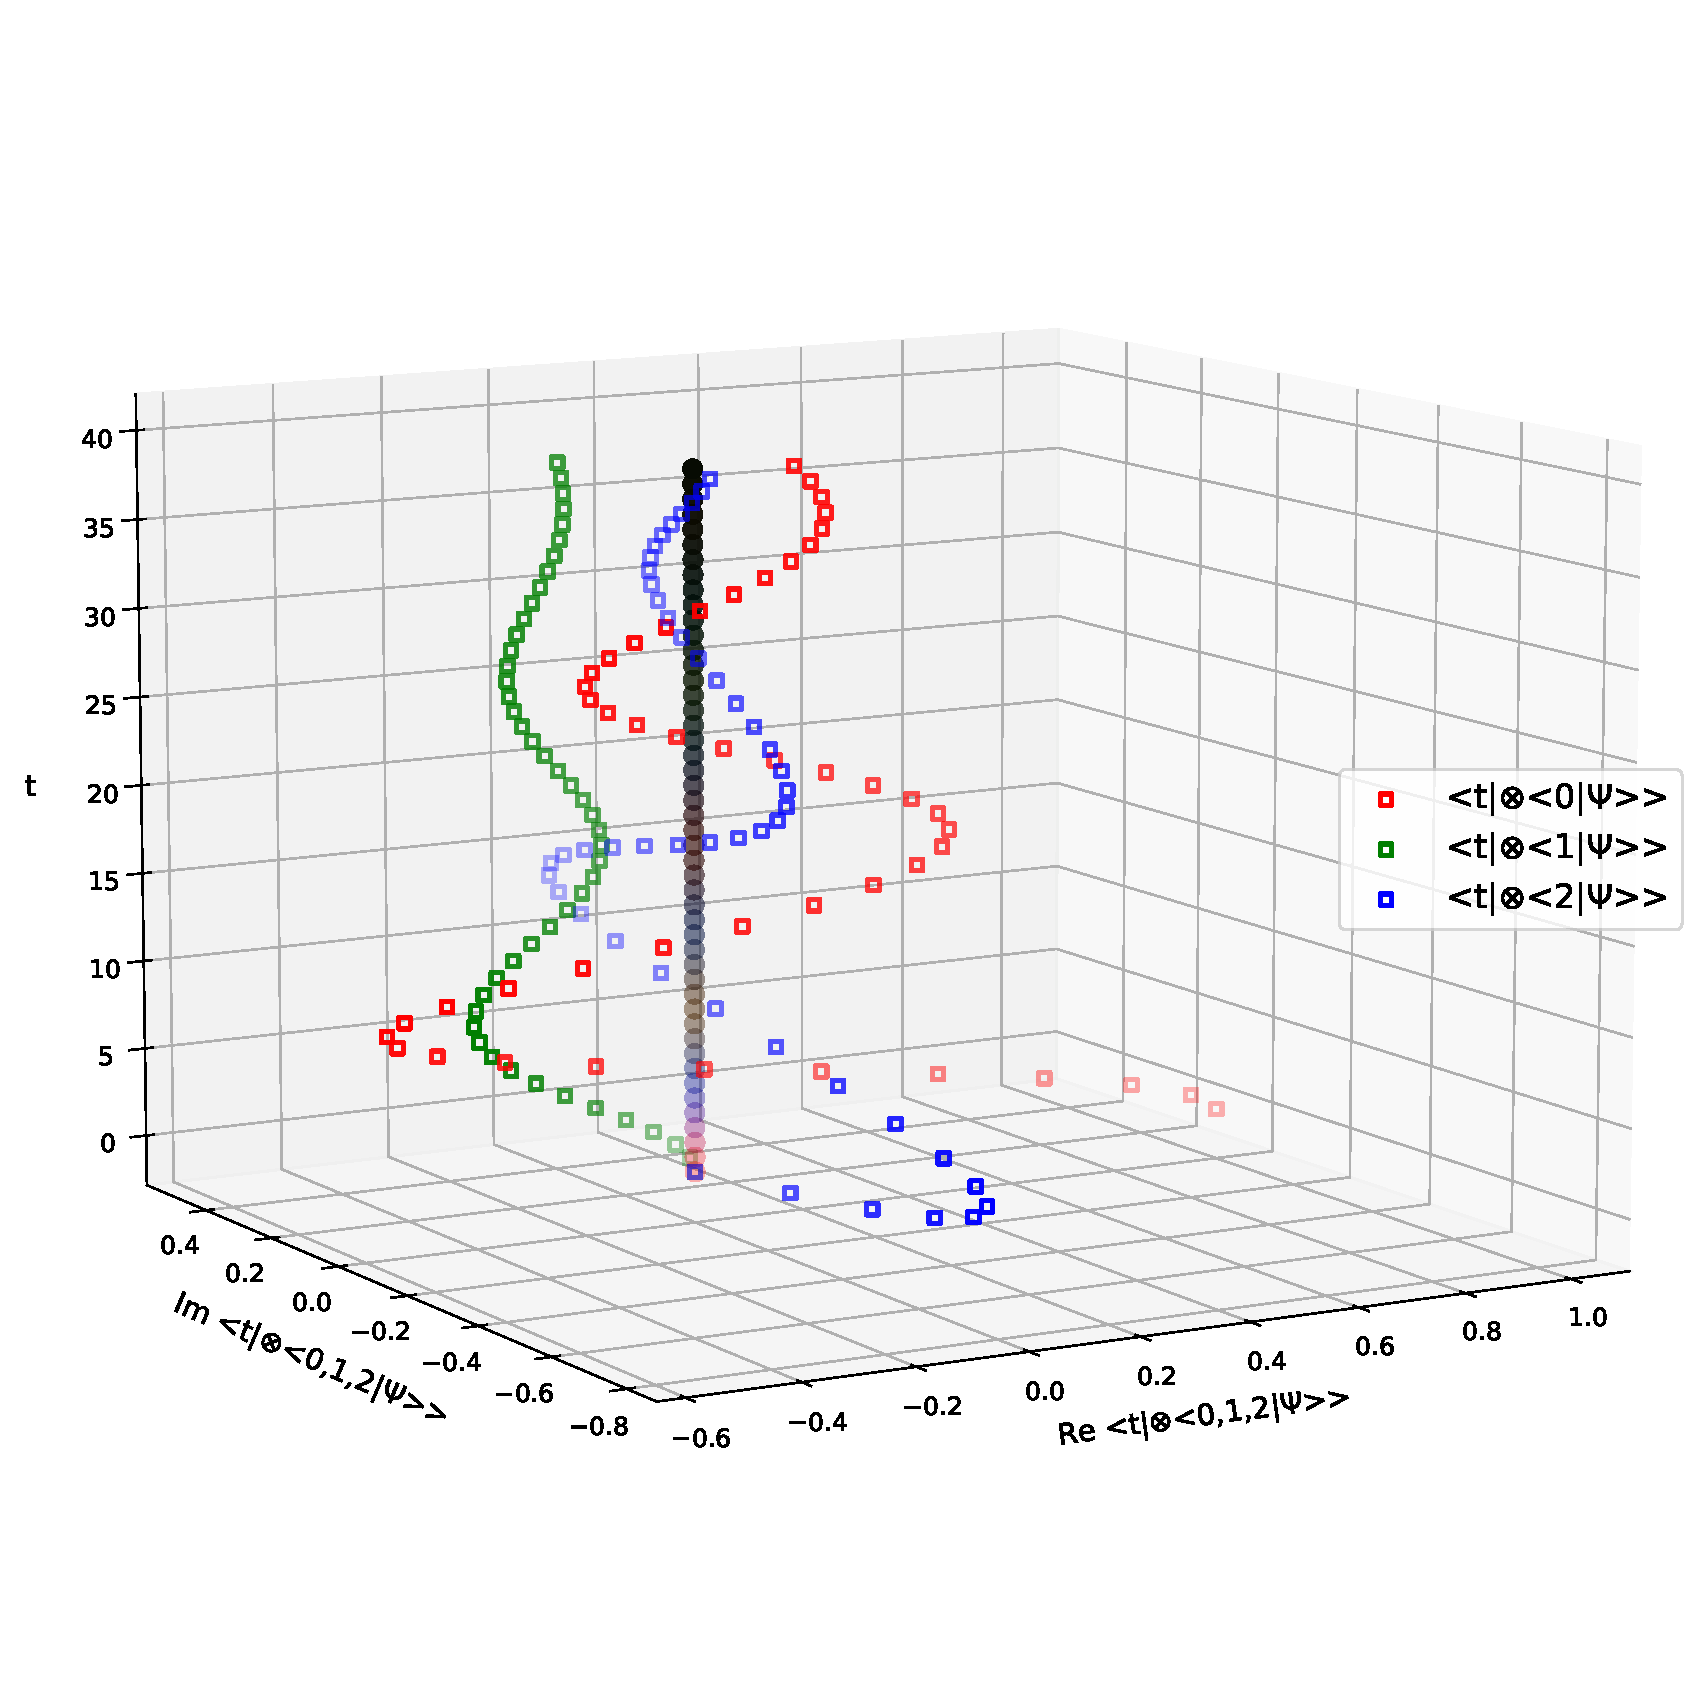
\includegraphics[height=0.41\textheight,clip,trim=0 90 0 140]{img/3ldetect/PWSpaceTime_side.pdf}
    \caption{3-D plot: side view.}
  \end{subfigure}
  \par\bigskip
  \begin{subfigure}[b]{\textwidth}
    \centering
    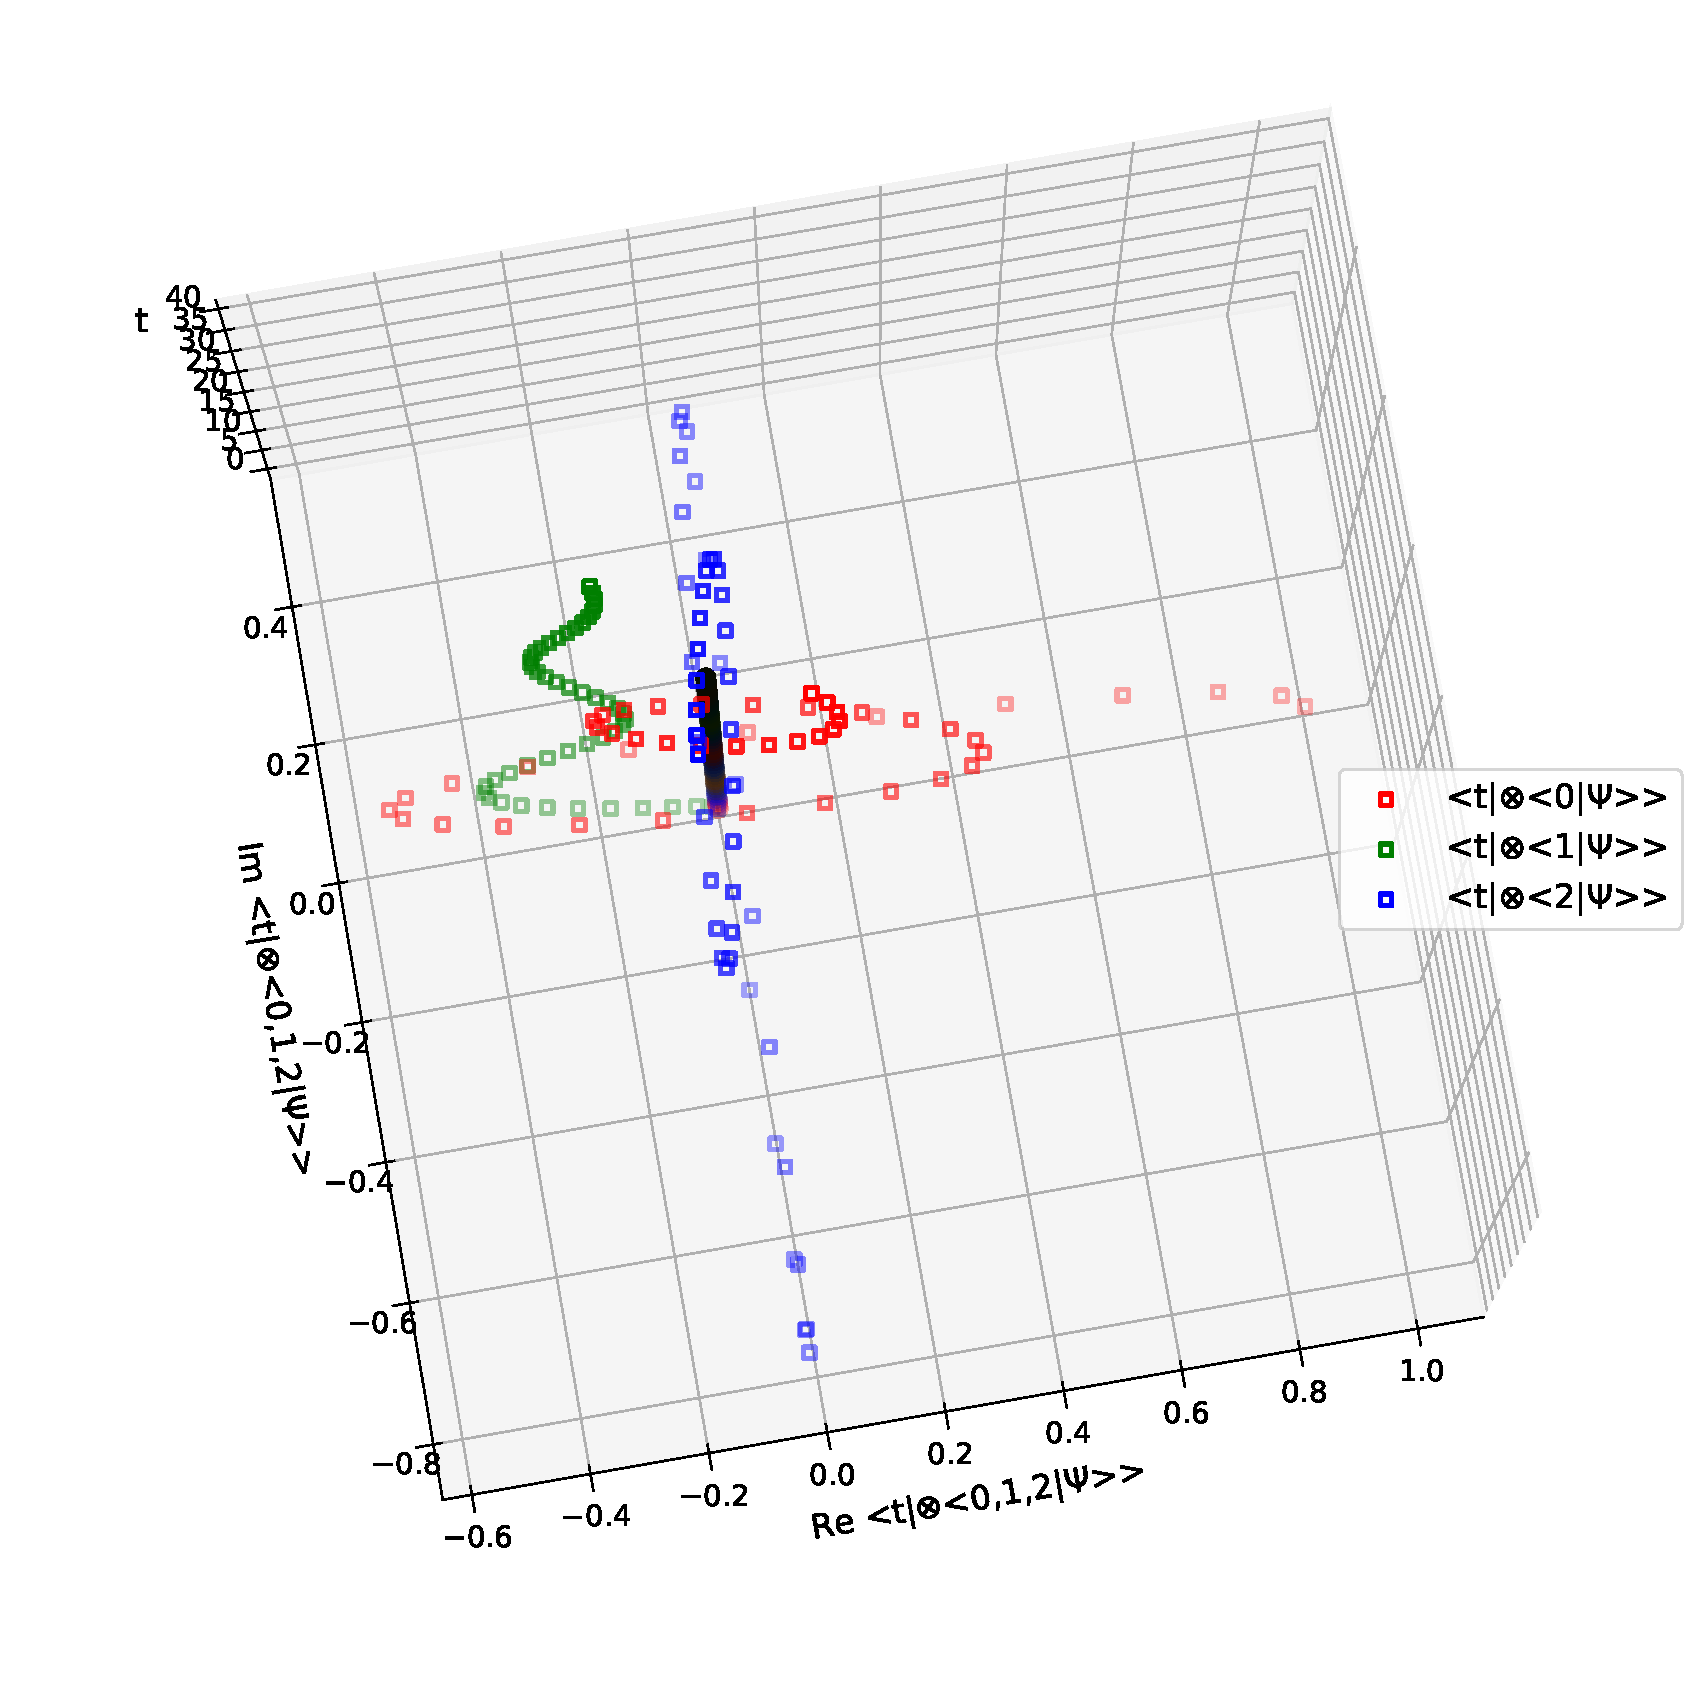
\includegraphics[height=0.48\textheight,clip,trim= 0 60 0 100]{img/3ldetect/PWSpaceTime_top.pdf}
    \caption{3-D plot: top view.}
  \end{subfigure}
  \caption[
    Components (complex values) of $\dket{\Psi} \in \pwspace$
  ]{
    Components (complex values) of the discrete-Page--Wootters vector
    $\dket{\Psi} \in \pwspace$
    (``evolution without evolution'').
    Can be compared with Fig.~\ref{fig:3lev:nonHermitianEvol}.
  }
  \label{fig:3lev:PWSpaceTime}
\end{figure}

% Uses dpfloat and \ContinuedFloat
\begin{figure}[p] % will be the left-side figure
  \begin{leftfullpage}
    \begin{subfigure}{\textwidth}
      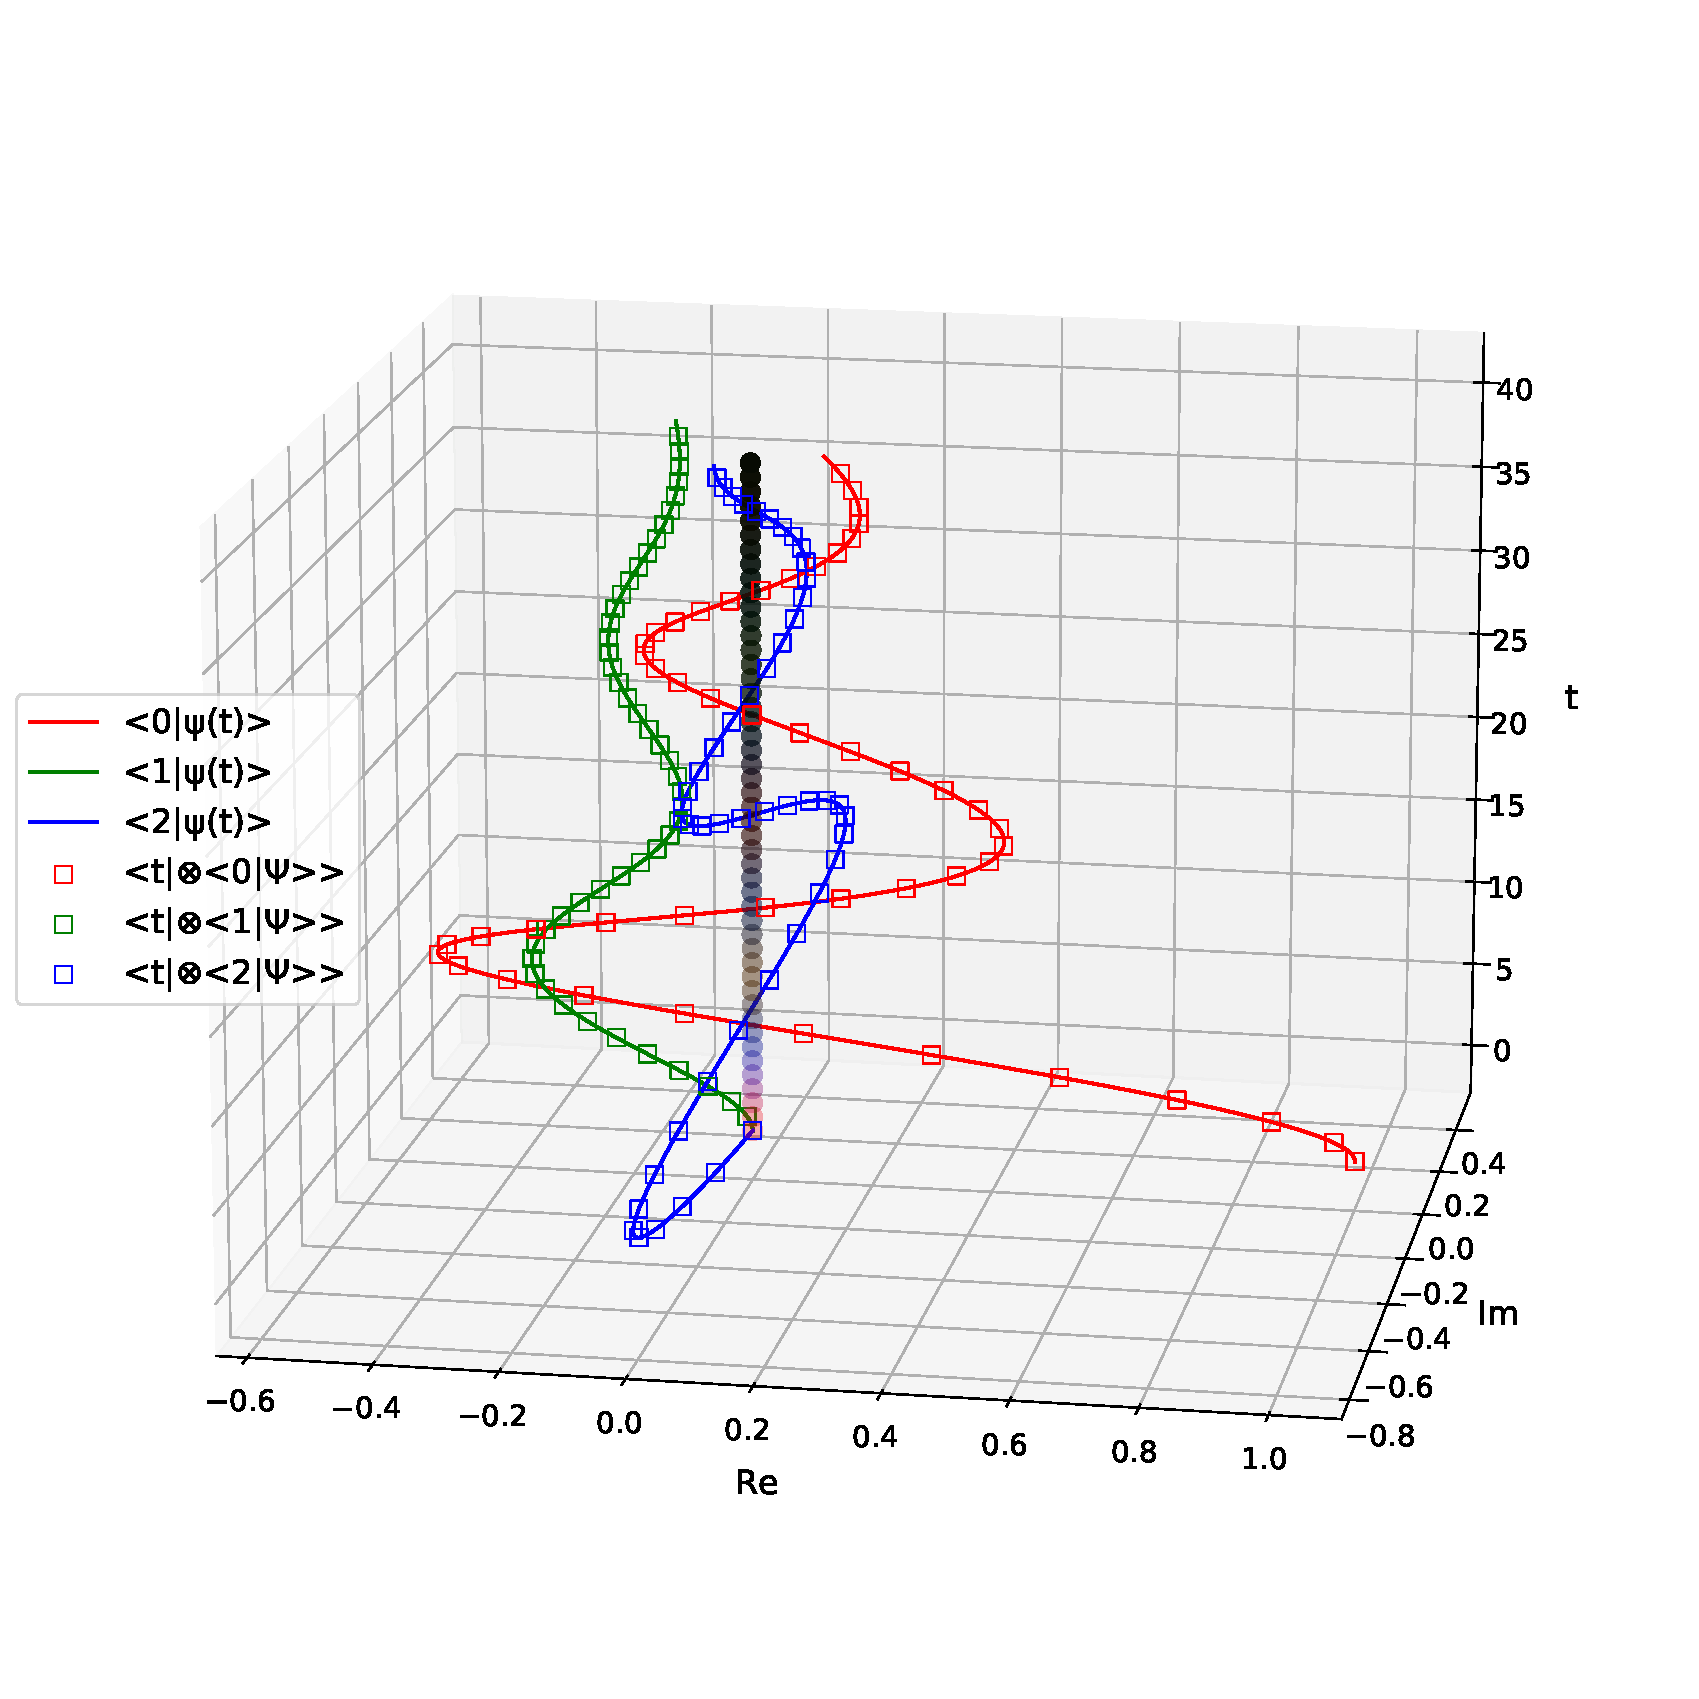
\includegraphics[width=\textwidth]{img/3ldetect/PWSpaceTimeFit_side.pdf}
      \subcaption{3-D plot: side view}
      \label{fig:3lev:PWSpaceTimeFit:side}
    \end{subfigure}
    \caption{
      Discrete Page--Wootters results (points)
      interpolate
      Schr\"{o}dinger
      evolution (continuous lines).
    }
    \label{fig:3lev:PWSpaceTimeFit}
  \end{leftfullpage}
\end{figure}
\begin{figure}[p]\ContinuedFloat % will be the right-side figure
  \begin{fullpage}
    \begin{subfigure}{\textwidth}
      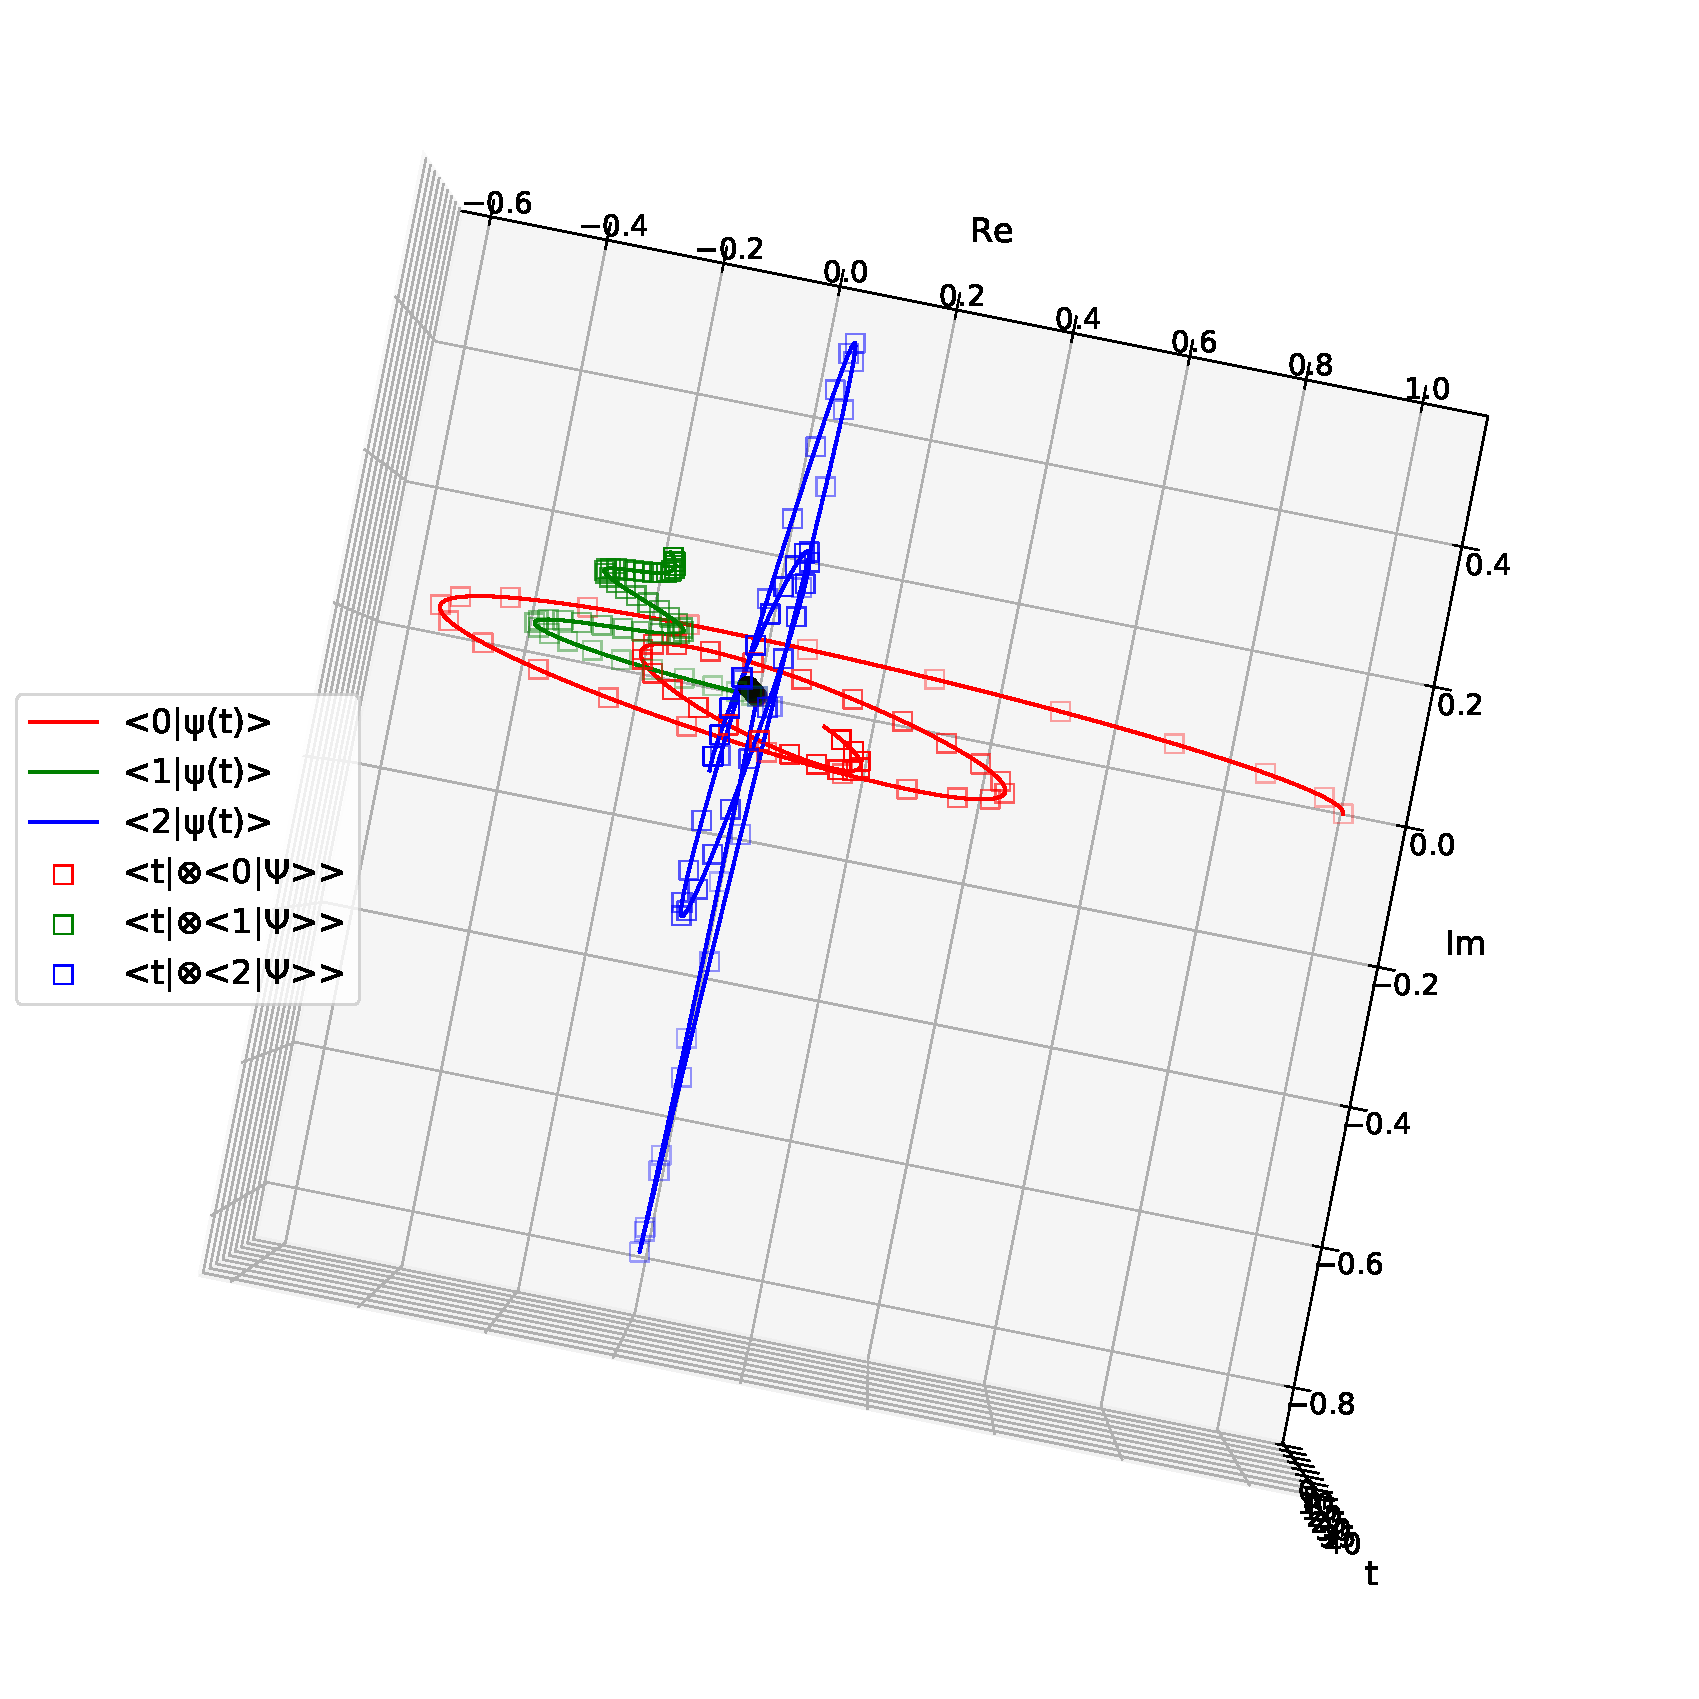
\includegraphics[width=\textwidth]{img/3ldetect/PWSpaceTimeFit_top.pdf}
      \subcaption{3-D plot: top view}
      \label{fig:3lev:PWSpaceTimeFit:top}
    \end{subfigure}
    \caption{
      \textit{Continued from Fig.~\ref{fig:3lev:PWSpaceTimeFit:side}}.
      Discrete Page--Wootters results (points)
      interpolate
      Schr\"{o}dinger
      evolution (continuous lines).
    }
  \end{fullpage}
\end{figure}

\subsection{Time-of-arrival (conditional) probability}

From \cite{Maccone:QMOT}, a time-of-arrival probability distribution can be derived
for the three-level system at hand, within the Page--Wootters formalism.
In a finite-dimensional
Hilbert space there's no notion of position or ``region of space'', but, as stated in the
same paper,
\begin{quote}
  [\dots] the whole discussion can be easily extended to the “time at which any
  event happens”. For example, if one considers a spin instead of a particle on a line, one can define the “time at
  which the spin is up”.
  
  [\dots] the notion of ``event'' in quantum mechanics [can be] defined as ``something that happens to a
  quantum system'', where ``something'' means ``a system
  observable property taking some value [\dots]''.
\end{quote}
Rather than spin up or down, in the present example, the arrival time at level $\ket{2}$
can be derived:
\begin{multline}\label{eq:3lev:bayesPW}
  P^{PW}(t_n|2) \eqbydef P^{PW}\Big( t_n \Big| 2, \left[0,\Delta{T}\right]\Big) = \frac{
    \abs{\bra{t_n} \ox \bra{2} \cdot \dket{\Psi}}^2
  }{
    \sum_{n'=0}^{N_{T} - 1} \abs{\bra{t_{n'}} \ox \bra{2} \cdot \dket{\Psi}}^2
  }
  \,\text{,}
  \\
  \text{ where } t_{n'} = n'\delta{T} = \frac{n'\Delta{T}}{N_{T}}
  \text{;}
\end{multline}
which gives the (conditional, \term{Bayesian}) probability that, given that a detection of $\ket{2}$
happens
within $t \in [0, \Delta T]$, it happens at time $t_n$ (or, more correctly, between $t_n$ and $t_{n+1}$).

On the other hand, and outside the Page--Wootters formalism,
within  the absorptive detector model
(see e.g. Sec.~\ref{sec:3lev:complexPotential} or Fig.~\ref{fig:3lev:loss})
the detection probability density reads $p(t) = - \dv{\norm{\psi}^2}{t}$.

Thus, the \emph{conditional} probability density that
---\emph{provided }a detection\footnote{
  Or measurement of related observable eigenvalue,
  or spontaneous decay from $\ket{2}$ as in Sec.~\ref{sec:detect:atomlaser}.
}
of the system at $\ket{2}$ happens within $t \in [0, \Delta{T}]$---
it does happen at a particular time $t$ is
\begin{equation}\label{3lev:condProb}
  p(t|2) \eqbydef p\big(t   \:\big|\:   2,[0,\Delta{T}]\big)
  =
  \frac{
    - \dv{\norm{\psi}^2}{t}
  }{
    \int_{0}^{\Delta{T}} - \dv{\norm{\psi}^2}{t'} \dd{t'}
  }
  =
  \frac{
    - \dv{\norm{\psi}^2}{t}
  }{
    \norm{\psi(0)}^2 - \norm{\psi(\Delta{T})}^2
  }
  \;\text{.}
\end{equation}

The ``state of arrival'' in \eqref{3lev:condProb} is $\ket{2}$
because the operator
in \eqref{eq:3lev:nonUnitaryH:antiHermitianTerm}
is essentially $\op{D} = \gamma \ketbra{2}$. The same
state has been chosen in \eqref{eq:3lev:bayesPW}
to allow a comparison. However, $P^{PW}(t_n|2)$ is a probability,
while $p(t|2)$ is a probability \emph{density}.
Therefore, the \eqref{eq:3lev:bayesPW} should be divided by $\delta T$,
i.e. the duration of the time interval the probability refers to,
before being plotted in Fig~\ref{fig:3lev:condProb},
where the two models show indeed fully compatible results.
\begin{figure}[]
  \centering
  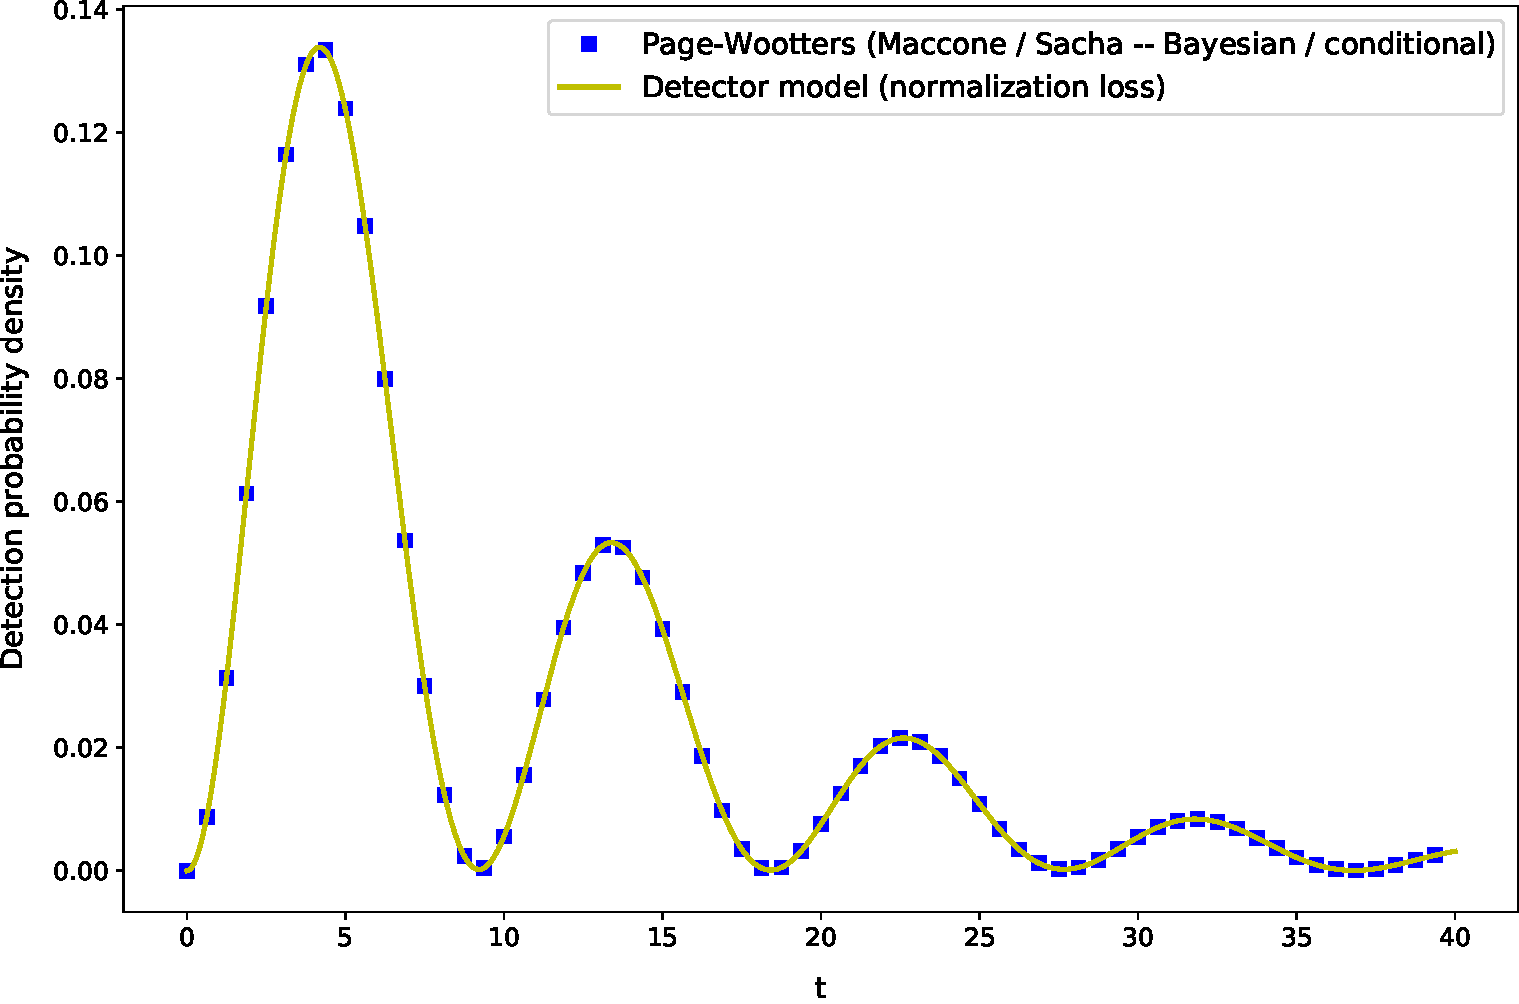
\includegraphics[width=\textwidth]{img/3ldetect/conditionalProbFit.pdf}
  \caption[
    Conditional probability density for time of arrival at state $\ket{2}$.
  ]{
    Conditional probability density for time of arrival at state $\ket{2}$.
    Discrete points: $P^{PW}(t_n|2) / \delta{T}$ (Page--Wootters).
    Continuous line: $p(t|2)$ (detector model).
  }
  \label{fig:3lev:condProb}
\end{figure}

\subsubsection*{\term{NumPy} code}

Relevant portion of code to compute the \eqref{eq:3lev:bayesPW} follows.
Values of probability density
$\frac{1}{\delta{T}}  P^{PW}(t_n|2)$
are stored in the array \Verb|Y|:
\begin{lstlisting}[language=Python]
# [...]
def tn_ox_arrived(n):
  # tensor product
  return np.kron(t_eigenstate(n), arrived_state)

history_normalized = history / norm(history)  ## normalized in H_T \otimes H_S

def joint_prob(n):
  return np.abs(tn_ox_arrived(n) @ history_normalized)**2

X = np.arange(NT)
iterable = (joint_prob(n) for n in X)
Y = np.fromiter(iterable, float)
dT  = DT / (NT)

# A "time bin"
X = X * dT # real time
Y = Y / dT # probability _density_

bayes_denominator = np.sum(Y * dT)
Y = Y / bayes_denominator
\end{lstlisting}

The \eqref{3lev:condProb} is partly implemented
directly in the plotting code:
\begin{lstlisting}[language=Python]
ax.plot(times, -np.gradient(norms**2, times) / bayesian_denominator_nonpw,
c='y', linewidth=2, label='Detector model (normalization loss)')
\end{lstlisting}
particularly with the expression
\lstinline{-np.gradient(norms**2, times) / bayesian_denominator_nonpw}.
The array \Verb!norms! was previously assigned values of $\norm{\psi(t)}$
while computing the non-unitary evolution for the problem in Sec.~\ref{sec:3lev:complexPotential}.
Here, explicitly:
\begin{lstlisting}[language=Python]
# [...]
def B(_t, _gamma=GAMMA):
  return expm(-1j*K(_gamma)*_t)

def non_unitary_psi(_t, _gamma=GAMMA):
  return B(_t, _gamma) @ psi_0

# [...]
_iter_norm = (norm(non_unitary_psi(_t)) for _t in times)
norms = np.fromiter(_iter_norm, np.float)
\end{lstlisting}
where, again, the function \Verb!K()! returns the matrix in \eqref{eq:3lev:nonUnitaryH}.
As per the ``Bayesian denominator'':
\begin{lstlisting}[language=Python]
# loss of normalization, or integral of antiderivative...
bayesian_denominator_nonpw = 1 - norm(evolution.T[NPLOTPOINTS-1])**2
\end{lstlisting}

Full code for this Section can be consulted at Appendix \ref{toa-prob-as-in-macconesacha-arxiv1810.12869}.


\chapter{Conclusions and Outlook}\label{ch:outlook}
\section{Discussion}

The initial draft title for this work was: 
\textit{It's $\it\ket{1}$ o'clock -- Relational Time and Applications}.
May time have eigenvectors and eigenvalues?
Indeed,
we have illustrated,
mainly through numerical examples
at various degrees of complexity,
and developing from existing theoretical work,
how time can be treated as a quantum observable
(described by a self-adjoint operator with its eigenvalues ---and eigenvectors).

The Pauli objection (presented in Section~\ref{proof})
can be overcome if the time operator $\hat{T}$
is defined in a different Hilbert space (that we name $\hilb{H}_T$),
distinct from
the space, say $\hilb{H}_S$, where the Hamiltonian is defined,
as set out by the Page and Wootters model
\parencite{PageWootters, Lloyd:Time, Marletto:Evolution, Maccone:QMOT, Maccone:Pauli}.

One can introduce an extra Hilbert space, to that of ordinary quantum mechanics,
in which the time operator is defined.
Or, more ``realistically'', identify, in a closed system, a subsystem
acting as a clock for the rest of it. Requirements are non-interaction and
full entanglement.

In terms of potential further development,
Section~\ref{sec:KG} introduces the possibility of a special-relativistic extension
by formulating the Klein--Gordon equation in Page--Wootters terms.
More possible lines of further research are mentioned in Section~\ref{sec:outlook-misc}.




\section{Relativistic formulation: Klein-Gordon}

The Klein-Gordon equation is the relativistic extension of the
(\emph{square of}) a wave equation for a free spinless particle.
Indeed, both sides have the dimension of
the square of an energy, and finding their square root
(in the operator sense) is non trivial task which was only resolved 
with the Dirac equation, from which the
intrinsic \term{spin} (particularly spin $\hbar/2$) logically emerges,
rather then being artificially introduced in the theory
to comply with the phenomenology
(\cite{Greiner_Rel}, \cite[Ch. 8]{Sakurai2}, \cite{DiracEquation}, \cite[handout 2]{Webber_notes}).

Both equations did not have much fortune as first-quantized equations,
for conceptual difficulties and historical reasons, including the rise
of Quantum Field Theory and second quantization. They do have a fundamental
role though as field equations (before quantization methods are enacted).
\parencite{PeskinSchroeder}.

The purpose of the present work is, in a sense, promoting time to a quantum
observable, or formally to a linear, self-adjoint operator in some Hilbert space.
The passage from quantum mechanics to field theory does not represent any progress
towards such goal, in that not only it does not ``promote'' time to an operator $\hat{t}$,
but it also ``demotes'' the three position operators $\hat{x}$, $\hat{y}$ and $\hat{z}$
to mere (classical) \emph{parameters}. However, consistently to relativistic covariance,
time and space coordinates are treated on equal footing. The Page and Wootters model
offers the opportunity to do the same, but both time and position are operators!

\subsection{Page and Wootters squared}

From the \eqref{eq:pwHamiltonian} and \eqref{eq:Wheeler-DeWitt}:
\begin{equation}\label{eq:pw_to_be_squared}
  -\hbar\hat{\Omega}\ox\idop_S \dket{\Psi} = \idop_T\ox\hat{H}_S \dket{\Psi} \,\text{.}
\end{equation}
Squaring the operators on both sides, we have:
\begin{equation}\label{eq:pw_squared}
  \hbar^{2}\hat{\Omega}^{2}\ox\idop_S \, \dket{\Psi} = \idop_T\ox\hat{H}_S^{2} \,\, \dket{\Psi} 
    = \idop_T \ox \left( \hat{p}^2 c^2 + m_0^2 c^4 \right) \dket{\Psi} \,\text{,}
\end{equation}
where the last equality is due to the ``quantization'' of the relation $E^2 = p^2 c^2 + m_0^2 c^4$
into $\hat{H}_S^{2} = \hat{p}^2 c^2 + m_0^2 c^4$.

We know from previous sections that in the $\qty{\ket{t}}_T$ basis $\hat{\Omega}$ is represented as
$-i\hbar\pdv{t}$. We know from standard quantum mechanics that in the $\qty{\ket{x}\ket{y}\ket{z}}_S$
basis is $\hat{p} \repr -i\hbar\nabla$. Therefore in the product basis the \eqref{eq:pw_squared} yields:
\begin{equation}\label{eq:proto_kg}
  -\hbar^2\pdv[2]{t}\Psi = \qty(-\hbar^2 c^2 \nabla^2 + m_0^2 c^4)\Psi
\end{equation}
which, up to some elementary algebra, is the well known \term{Klein-Gordon equation}.

In standard quantum mechanics (first quantization, relativistic or not)
\begin{equation}
  \ket{\psi(t)} = \int \dd{x}\dd{y}\dd{z} \Psi(x,y,z;t) \ket{x}\ox\ket{y}\ox\ket{z} \,\text{.}
\end{equation}
In this formulation
\begin{equation}
  \dket{\Psi} = \int \dd{x}\dd{y}\dd{z}\dd{t} \Psi(x,y,z,t) \ket{x}\ox\ket{y}\ox\ket{z}\ox\ket{t} \,\text{,}
\end{equation}
and $t$ is no longer a classical parameter, but an eigenvalue of the time operator,
or a label for time basis elements. Please note that, as a function of four variables,
$\Psi$ is not normalizable i.e. it's not a proper element of
$\mathcal{L}^2(\mathbb{R}^4)$
(normalization issues are tackled in \cite[eq. 23 and following]{Lloyd:Time}).

\subsection{Covariant notation}

The \eqref{eq:proto_kg} can be rearranged and expressed in explicitly covariant form:
\begin{equation}
  \qty[\partial_{\mu}\partial^{\mu} + \qty(\frac{mc}{\hbar})^2]\Psi = 0
\end{equation}
with standard relativistic notation.
Similarly
---at operator level, in the tensor product space---
the \eqref{eq:pw_squared} can be rearranged:
\begin{equation}\label{eq:pwkg}
  \qty[- \hat{\mathrm{P}}_{\mu} \hat{\mathrm{P}}^{\mu} + \qty(\frac{mc}{\hbar})^2]\Psi = 0
\end{equation}
with
\begin{equation}
\begin{aligned}\label{eq:p0123}
  \hat{\mathrm{P}}_0 &=& \frac{\hbar\hat{\Omega}}{c}  \ox \idop_x   \ox \idop_y   \ox \idop_z \\
  \hat{\mathrm{P}}_1 &=& \idop_T                      \ox \hat{p}_x \ox \idop_y   \ox \idop_z \\
  \hat{\mathrm{P}}_2 &=& \idop_T                      \ox \idop_x   \ox \hat{p}_y \ox \idop_z \\
  \hat{\mathrm{P}}_3 &=& \idop_T                      \ox \idop_x   \ox \idop_y   \ox \hat{p}_z
\end{aligned}
\end{equation}
and the usual relation between contravariant and covariant 4-vectors:
\begin{equation}
  a_\mu = \eta_{\nu}^{\mu} a^{\nu} \text{;} \quad
  \eta = \mathrm{diag}(+1, -1, -1, -1)
  \text{.}
\end{equation}

It's tempting to name the \eqref{eq:pwkg} and \eqref{eq:p0123} the \term{Page-Wootters-Klein-Gordon}
equation.\footnote{
  Or \term{Klein-Gordon-Wheeler-DeWitt-Page-Wootters-Giovannetti-Lloyd-Maccone}
  equation, thus giving
  credits to all authors, particularly if we consider that the idea of an extra Hilbert space
  was conceived originally in \cite{Lloyd:Time}.
}

As anticipated, this resolves the asymmetry in Tables \ref{op_comparison_alg} and \ref{op_comparison_J},
whereas we can write
{
  \begin{table}[h!]
    \centering
    \begin{tabular}{p{0.3\linewidth}||c|c|c}
                                                                                &
        $\hilb{H}_T$                                                            &
        $\hilb{H}_S$                                                            &
        {\footnotesize Mass term}                                               \\
      \hline
      \hline
        {\footnotesize Spatio-temporal ``positions''}                           &
        $\hat{t}$                                                               &
        $\hat{x}$                                                               &
                                                                                \\
      \hline
        {\footnotesize Canonically conjugate}                                   &
        $\hat{P_0} = \frac{\hbar\hat{\Omega}}{c} \repr -i\partial_{0}$          &
        $\hat{P}_{1,2,3} \repr -i\nabla$                                        &
                                                                                \\
      \hline
        {\footnotesize Dynamics (terms in the Wheeler-DeWitt equation)}         &
        $\hat{P}_{0}\hat{P}^{0} \repr -\hbar^2 \partial_{0}\partial^{0}$        &
        $\hat{P}_{j}\hat{P}^{j} \repr -\hbar^2 \partial_{j}\partial^{j}$        &
        $\qty(\frac{mc}{\hbar})^2$
    \end{tabular}
    \caption{
      Operators in the space-time Hilbert spaces.
    }
  \end{table}
}
\section{An intro chap on motivation and experiments?}
\begin{itemize}
  \item Time crystals?
  \item Time-resolved diffraction patters, temporal double slit experiment + Muga theory \url{https://arxiv.org/abs/0812.3034}
\end{itemize}

%\clearpage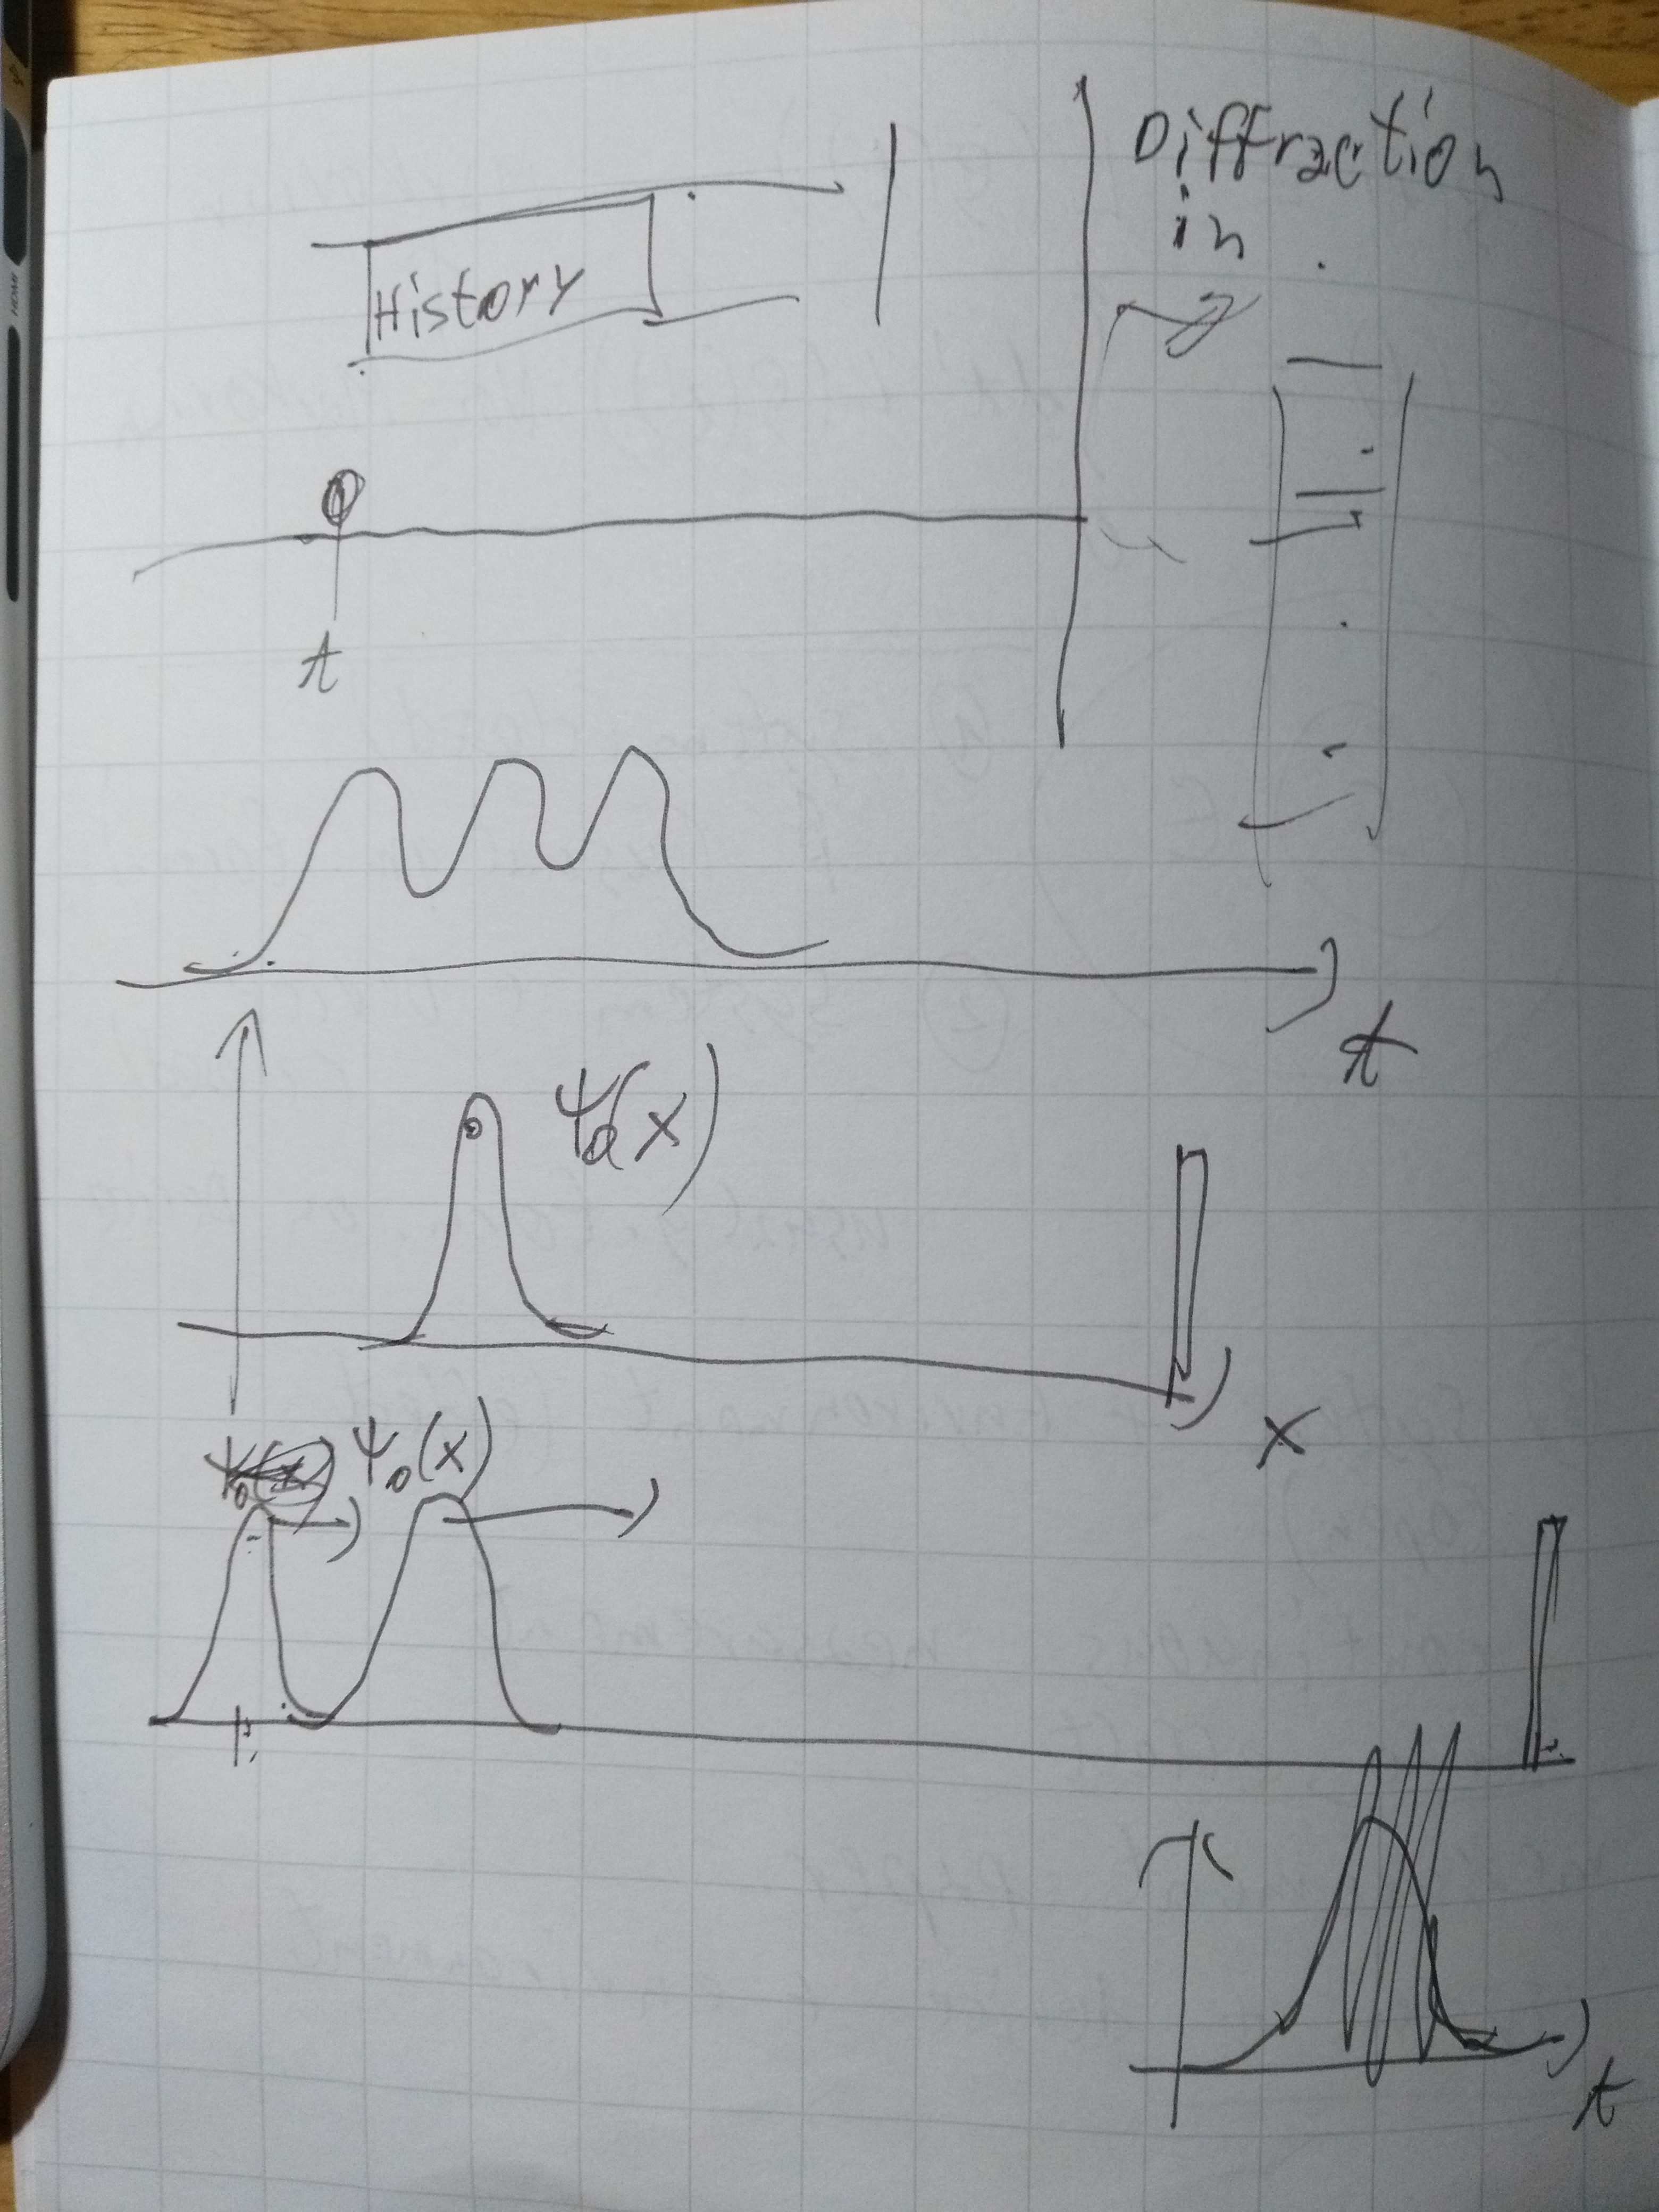
\includegraphics[width=\linewidth]{img/diffraction.jpg}

\section{Misc}


\subsection{Half-line spectrum}
Even if time was bounded from below (Big Bang), that would not invalidate the \textbf{Pauli objection}.
(Look at the proof of Pauli objection).
Though, it would be worth mentioning the momentum in the half-line (Ruschhaupt)
and develop some considerations then\dots


\subsection{Quantum computing, IBM, decomposition, Trotter-SUzuki, Sine-cosine, qubiter dir}

Previous section(s) read(s):
\begin{quote}
  A benefit of finite-dimensional systems is the potential implementation on a finite array of
  qubits in a quantum computer.
\end{quote}
Make a ref from there to here, and talk about qubiter and stuff.

Also, \cite{Moreva:illustration} has FIG.1 gate array repr\dots

\subsection{Quantum Blockchain and Entanglement in Time}

\url{https://spectrum.ieee.org/tech-talk/computing/networks/quantum-blockchains-could-act-like-time-machines}
\url{https://arxiv.org/abs/1804.05979}


\subsection{Misc}

Extra: \cite{TimeAnyons}.

TQM Book: time of residence: applicable to qubits, therefore Moreva experiment.

\url{https://arxiv.org/abs/1708.04302} majorization, thermo.


\subsection{and dwell time}

\cite[sec.5]{TQM2}, \cite{YearsleyHalliwell_Clocks}. (create an @inbook for this)

\subsection{In relation with the \term{time of residence}}

Here we compare \cite{Moreva:synthetic, Moreva:illustration}
(a Page and Wootters problem)
with the ``standard'' \term{time of residence}
treated in \cite[sec.5.5.2]{TQM2} (create an @inbook for the chapter), 
the only usable concept since there is no notion of position
for a qubit. This can also be connected with the time-slices
in the notion of conditional time-of-arrival probability  by Leon and Maccone
which is used in the jupyter notebook.

\subsection[Comparison with Kijowski/Aharonov-Bohm]{Comparison with (Kijowski/Aharonov-Bohm) time of arrival}

Time of arrival is derived for non-relativistic \parencite{Delgado_TOA, Delgado_TOA2}
and relativisitic \parencite{Leon_TOA_R}
particle.

Kijowski: \cite{Kijowski_Time, Kijowski_Comment}.

\subsection{In relation to Leggett-Garg inequalities}
(Also mentioned in \cite{Moreva_position}).

Ref \cite{LeggettGarg+PageWootters}.

But also Lloyd: \url{https://arxiv.org/abs/1608.05672},
\emph{Decoherent histories approach to the cosmological measure problem}.
Lindbladt, Markov, Open Systems.

Halliwell, \url{https://arxiv.org/abs/1604.01659}. Ancilla, decay (spontaneous emission?).

A phylosophical object to decoherent histories / Everett (Everett mentioned in Marletto/ref)
is at
\url{https://arxiv.org/abs/1603.04845}.



\subsection[On ``taking time seriously'']{On ``taking time seriously'' (time is real) and why it can still be real in Page and Wootters}

No, Smolin
(\term{Time Reborn}, \term{The Singular Universe and the Reality of Time})
pushes this too far, even Special Relativity's time is too ``virtual'' for him.
Similarly, the philosopher Tim Maudlin

\url{https://www.quantamagazine.org/a-defense-of-the-reality-of-time-20170516/}

Here instead we just argue that the clock can actually be really time, not any observable.
We use notation $T$ as in time instead of $C$ as in clock etc.

In this sense, the Moreva experiment is a quantum analogue simulation.


\section{Time crystals}

References: \cite{crystal2,crystal3,crystal2012}.


\section{Irrev}

\cite[sec.IV.  UNBOUNDED-ENERGY CLOCKS?]{Maccone:Pauli}

\subsection{Use open quantum systems theory in ``Decoherence and measurement'' chapter + Entropy}
Schmidt decompositions, spatial and temporal states in
$\hilb{H}_T$ and $\hilb{H}_S$
are described as density operators
(mixed states).

This has been actually used to prove clock time-frequency uncertainty relation
in terms of mixture.

What if there isn't a ``perfect entanglement'' between space and time.

Use the Von Neumann entropy (or other methods) to quantify entanglement?

When the entanglement is perfect, the notion of time evolution emerges, just
like between two dimensions in space, it may or may not ``emerge'' that
$y$ ``depends'' upon $y$ for a given distribution of positions.

Where the entanglement is maximal, the Von Neumann entropy is also maximal.

Arrow of time as increasing entanglement (and entropy!). See Also
\cite{Marletto:Evolution}.
Connect this with our jupyter notebook with complex potential: Marletto mentions
clock + rest, and rest = observed + observer. Think ``observed'' is the atom
and ``observer'' is the photon bath. Their entanglement increases as
more photon are spontaneously (i.e. irreversibly) emitted.
One might want to study the atom+photon system exactly,
with explicit density matrices also,
instead of using
complex potential/quantum jump etc.

Also Lloyd recent on entropic uncertainty (for time\dots \cite{Lloyd:Entropic}).
Maybe also \cite{Wehner:Uncertainty}.

Subadditivity.

\subsubsection{Quantifying entanglement}

Vedral: \url{https://arxiv.org/abs/quant-ph/9702027}.

Jon Yard, entropy: \href{http://www.perimeterinstitute.ca/fr/videos/quantifying-entanglement-quantum-entropy}{Perimeter video}.

Caterina-Eloisa Mora, ``beyond'':
\href{https://www.perimeterinstitute.ca/videos/quantifying-quantumness-correlations-beyond-entanglement-and-back}{Perimeter video},
\href{https://arxiv.org/search/advanced?advanced=&terms-0-operator=AND&terms-0-term=Mora%2C+caterina-eloisa&terms-0-field=author&terms-1-operator=OR&terms-1-term=mora%2C+c+e&terms-1-field=author&classification-physics_archives=all&classification-include_cross_list=include&date-filter_by=all_dates&date-year=&date-from_date=&date-to_date=&date-date_type=submitted_date&abstracts=show&size=50&order=-announced_date_first}{arXiv search}.

Geometric measure: \url{https://arxiv.org/abs/quant-ph/0307219}.

``Resources'': \url{https://arxiv.org/abs/1402.6710}.

\section{Entanglement and decoherence (Arrow of time)}
See also \cite{EntanglementVsDecoherence}.

Decoherence is an irreversible process, it also happens in measurement.

According to Marletto and Vedral, arrow of time is increase in Entanglement
between the clock and the rest.

So, there seems to be a contradiction: is entanglement ``decreasing''
(i.e. destroyed by decoherence) with time
or increasing?

We can avoid the contradiction saying that
entanglement between two finite systems is
destroyed while the entanglement of each of them with the universe
is increasing.

\subsection{``Harmonic clocks''}

Use the harmonic oscillator in \cite{HarmonicClocks}
as a PaW clock for the same packet that is measured in
Ruschhaupt's detector model.

Therein, fading wave function: is minus derivative an event?
L4 normalized?

\subsection{Atomic clocks / quantum clocks}
Technologically implemented! There is a section in the intro chapter of the book,
\emph{and} a dedicated chapter.

\subsection{Misc}

Idea: use section B ``Measurement'' of \cite{Lloyd:Time}: detector as (binary) measument device.

``Philospher'': \url{https://arxiv.org/abs/1704.07236}.

Time of arrival and clocks: again, \cite{YearsleyHalliwell_Clocks}.
Which maybe suggests we should not worry too much of $H\ket{\Psi} = 0$.

We don't.

BUT please note \cite{YearsleyHalliwell_Clocks} uses a clock that is
\emph{coupled} with the system, while in PaW they are ``only'' entangled.
So their calculation may be unnecessarily complicated.
Maybe the weakjly coupling case can be used?

Other systems of interest: decays. Prvanovic new.

Reference \cite{ConnesRovelliThermo}.

Relate with John Goold's works? The ancilla as a clock? --- Topical Review

Markovianity, histories.

Lloyd on arXiv: from clock to cloners; erasing; scrambling (as in Goold).

Lloyd on decoherent histories (Gellman, Hartle?).

Dechoerence / irreversibility / measurement.

Vedral / Lloyd. Discord.

Measuring entanglement: Quantification of Concurrence via Weak Measurement: 1611.00149.

Marletto/Vedral on Arrow of time. Arrow of time as increasing entanglement.

Arrow of time:

\url{https://www.wired.com/2014/04/quantum-theory-flow-time/}

\url{https://en.wikipedia.org/wiki/Loschmidt%27s_paradox}

\url{https://www.quantamagazine.org/20160119-time-entanglement/}

\url{https://arxiv.org/pdf/1702.07706.pdf} \textit{The second law of thermodynamics at the microscopic scale}
Thibaut Josset,
Aix Marseille Univ. (David).

Maxwell's demon: https://arxiv.org/pdf/1702.05161.pdf

\subsection{and paths}

Both \cite{YearsleyHalliwell_Clocks} and \cite{Gambini_PW}
reason in terms of paths and actions, maybe Feynmann stuff
in following chapter... and maybe conistent historiesapproach can help
towards linking PaW and ToA?

Also \url{http://quantum.phys.cmu.edu/CHS/CHS_transp.pdf}.

\subsection{Decays?}

We might want to look at exponential decay from \url{https://arxiv.org/abs/1704.07236},
then compare with exponential decay with P and W using Lloyd Giovannetti and Maccone (ref).

\subsubsection{Purification}

See https://arxiv.org/pdf/quant-ph/0512125.pdf, P-W time as a purifying ancilla
of the (Kijowski?) time.

\section{Misc/Multi/Extras/Outlook}

\url{https://arxiv.org/abs/1703.05876}
--- \emph{comment}: time measured and stored here
may be all classical information
so this paper may or may not be relevant for the topic.

But
``prototypes of clocks based on quantum principles,
such as entanglement and squeezing''
may make this interesting again, see reference therein.
They also cite Lloyd, Giovannetti and Maccone,
but a paper quite older than \cite{Lloyd:Time}.

\url{https://arxiv.org/abs/1603.02522}
\emph{Decoherence by spontaneous emission: a single-atom analog of superradiance}.
Decoherent histories, non-markovianity, open quantum systems.

\url{https://arxiv.org/abs/1007.2615} Time travel / Quantum CTC.

Carmichael et al. \cite{CarmichaelOQS2017} (Andreas's reading)
(non-markovianity).

Non-markovian, quantum-to-classical, open systems, David,
\url{https://arxiv.org/pdf/1703.09428.pdf}.

In his works, Zurek mentions:
DeWitt, Everett, gell_Mann, hartl, Many Worlds, consistent/decoherent histories:
idea: Lagrangian over a history? Principle of least action?

Zurek: ``Reduction of the Wavepacket: How Long Does it Take?'' (arxiv),
``quantum''' time? \cite{Zurek_Einselect} also mentions
``decoherence timescale''.

Von Neumann/Shannon entropy in measurement? Mention information problems
in quantum cosmology (where a quantum time is necessary)? Etc. etc.

\section{for Relativistic treatment}

Lorentz (+Galilei?) transformation. Lorent/Poincare groups. May be Important:
see \cite{LocalizationEntanglmentRelativistic}.

\cite{Misra}? Cited in TQM book 1 chap. 1 as 
``a different way out in the context of a theory of irreversible evolution''.
Mentions Klein-Gordon and Poincare group.

\cite{RealisticClocks}.

\cite{HarmonicClocks} concludes ``Classical clock can be described by an Hamiltonian linear in momentum''\dots
like in relativity?

\cite{Lloyd:Time} does not only deal with improper eigenstates in $\hilb{H}_T$
(full evolutions?)
but also normalized ones (in $\hilb{H}_T$! \emph{``Events''}?)

A Page and Wootters time of arrival is mentioned in \cite{Gambini_PW}.

\subsection{Time-of-arrival for a Klein-Gordon free particle}

See \cite{Galapon_KG}.

\subsection{Dirac eq.}

\url{https://arxiv.org/pdf/1502.00322.pdf}



\subsection{Feynmann path stuff}

Sokolovski 1703.01966, Feynmann paths...\subsection{(dis)entanglement under gravity, decoherence, event formalism}

1703.08036 An experiment to test decoherence under gravity aka entangled photons undergoing different paths and how their entanglement is affected.
``Space QUEST mission proposal: Experimentally testing decoherence due to gravity''.

Are they getting entangled with the environment instead? (Merletto and Vedral).

The theoretical paper behind the space experiment: \url{https://arxiv.org/pdf/1406.3677.pdf}. Interestingly, it mentions 
\emph{event formalism}, and we thought about that: is an event something
representable as a proper vector in $\mathscr{L}^2(\mathbb{R}^4)$ --- where one of the dimensions is time?
Deepen the event formalism if it's quantum.

Resume ``Quantum Statistical Gravity''? \url{https://arxiv.org/abs/1602.05707}.

``Fundamental decoherence from quantum gravity: a pedagogical review''
\url{https://arxiv.org/abs/gr-qc/0603090} ---
``fundamental loss of unitarity
that appears in quantum mechanics
due to the use of a physical apparatus to measure time''.

Closed timelike curves are also the subject of a paper by Lloyd (cite!).

``Deutsch argued that
the usual paradoxes associated with such solutions of general
relativity can be resolved by quantum mechanics''  in the reference above. But in the even formalism
\emph{spacetime is still a classical background!}. Event operators a parametrized by $t$\dots

\subsection{Prvanovic and P\&W}
In \cite{Prvanovic}, essentially the clock observable is the Hamiltonian.
The two example clocks are an harmonic oscillator and a free particle.
The harmonic oscillator features discrete time. Generally a time which is
{bounded from below}
is consistent with the Big Bang...

Prvanovic uses ``relativisitc'' constants...

BTW, please note a time bounded from below WOULD NOT be sufficient to overcome the Pauli objection alone.

\section{Photon position}

Quantum mechanics is a 0+1 QFT \parencite{QFT_0+1}.
The \emph{dimension} of the field theory is the number of external parameters.
The P-W mechanism ``quantizes'' external parameters, or make their property
of classical external parameter \emph{emerge} out of a quantum observable
of an entangled subsystem (where there exists a Schmidt decomposition over
eigenstates of said observable).

In this sense, time in quantum mechanics is like time \emph{and position}
in quantum field theories such as quantum optics or the Standard Model.

We can imagine P-W ``meter sticks'' instead of clocks, to measure
photon position and thus tackle the same problem of \cite{HawtonPhotonPosition}.

\section{Photon \emph{absorption}}

Photons are physically/really absorbed (or \emph{emitted}), although under a different theoretical framework
(second quantized Vs QM). No need of complex potentials\dots Connect with spontaneous emission?

Spontaneous emission/decay compared with PW (Maccone) and Kiukas (detection).
Perhaps Prvanovic article on spontaneous decay?


% appendices
\appendix

\chapter[Jupyter Notebooks]{Jupyter Notebooks\footnote{
  For a reference on the software tools utilized:
  \cite{comp:scipy};
  \cite{comp:sympy};
  \cite{comp:jupyter};
  \cite{comp:matplotlib};
  \cite{comp:numpy}.
}}
\section*{Technical note}

Original files available at
the code repository, ref. \cite{OwnJupyterRepo}.

Printable and embeddable \TeX{} files have been generated with
\begin{itemize}
  \item
    ``Download as Markdown''\footnote{
      This may not work if \term{Jupytext} \parencite{Jupytext} is used,
      although manual embedding of
      Python code in verbatim blocks or similar should be easier, as Python code 
      is available ``as is''.
    }
    from Jupyter user interface
  \item
    Installing and running \verb#pandoc#\footnote{ \url{http://pandoc.org/}}
    on the generated \verb#.md# file\footnote{ See also \url{https://tex.stackexchange.com/a/314785}.}
    \begin{lstlisting}[language=Bash]
      pandoc --listings -f markdown -t latex myfile.md -o myfile.tex
    \end{lstlisting}
  \item
    Tweaking generated \verb#\label#'s and other references as needed to avoid inconsistencies and overlaps
\end{itemize}

%\section{Commutator of finite-dimensional conjugate operators}\label{sec:jpynb:finite-comm}

\begin{lstlisting}[language=Python]
from sympy import *
from sympy.matrices.expressions.fourier import DFT
from sympy.physics.quantum.dagger import Dagger
\end{lstlisting}

\begin{lstlisting}[language=Python]
# Remeber this to have LaTeX rendered output in Jupyter
init_printing()
\end{lstlisting}

\begin{lstlisting}[language=Python]
N      = Symbol(r'N', real=True)
deltaT = Symbol(r'\delta{T}', real=True)
DeltaT = Symbol(r'\Delta{T}', real=True)
T      = Symbol(r'T')
F      = Symbol(r'F')
Omega  = Symbol(r'\Omega')
\end{lstlisting}

\begin{lstlisting}[language=Python]
N = Integer(4)
\end{lstlisting}

\begin{lstlisting}[language=Python]
deltaT = Rational(1, 1)
\end{lstlisting}

\begin{lstlisting}[language=Python]
DeltaT = N * deltaT
\end{lstlisting}

\begin{lstlisting}[language=Python]
T = diag(*Range(N))
\end{lstlisting}

\begin{lstlisting}[language=Python]
T
\end{lstlisting}

\(\displaystyle \left[\begin{matrix}0 & 0 & 0 & 0\\0 & 1 & 0 & 0\\0 & 0 & 2 & 0\\0 & 0 & 0 & 3\end{matrix}\right]\)

\begin{lstlisting}[language=Python]
F = DFT(N)
\end{lstlisting}

\begin{lstlisting}[language=Python]
F.as_explicit()
\end{lstlisting}

\(\displaystyle \left[\begin{matrix}\frac{1}{2} & \frac{1}{2} & \frac{1}{2} & \frac{1}{2}\\\frac{1}{2} & - \frac{i}{2} & - \frac{1}{2} & \frac{i}{2}\\\frac{1}{2} & - \frac{1}{2} & \frac{1}{2} & - \frac{1}{2}\\\frac{1}{2} & \frac{i}{2} & - \frac{1}{2} & - \frac{i}{2}\end{matrix}\right]\)

\begin{lstlisting}[language=Python]
Dagger(F).as_explicit()
\end{lstlisting}

\(\displaystyle \left[\begin{matrix}\frac{1}{2} & \frac{1}{2} & \frac{1}{2} & \frac{1}{2}\\\frac{1}{2} & \frac{i}{2} & - \frac{1}{2} & - \frac{i}{2}\\\frac{1}{2} & - \frac{1}{2} & \frac{1}{2} & - \frac{1}{2}\\\frac{1}{2} & - \frac{i}{2} & - \frac{1}{2} & \frac{i}{2}\end{matrix}\right]\)

\begin{lstlisting}[language=Python]
Omega = (Dagger(F) @ T @ F).as_explicit()
\end{lstlisting}

\begin{lstlisting}[language=Python]
Omega
\end{lstlisting}

\(\displaystyle \left[\begin{matrix}\frac{3}{2} & - \frac{1}{2} + \frac{i}{2} & - \frac{1}{2} & - \frac{1}{2} - \frac{i}{2}\\- \frac{1}{2} - \frac{i}{2} & \frac{3}{2} & - \frac{1}{2} + \frac{i}{2} & - \frac{1}{2}\\- \frac{1}{2} & - \frac{1}{2} - \frac{i}{2} & \frac{3}{2} & - \frac{1}{2} + \frac{i}{2}\\- \frac{1}{2} + \frac{i}{2} & - \frac{1}{2} & - \frac{1}{2} - \frac{i}{2} & \frac{3}{2}\end{matrix}\right]\)

\begin{lstlisting}[language=Python]
T @ Omega - Omega @ T
\end{lstlisting}

\(\displaystyle \left[\begin{matrix}0 & \frac{1}{2} - \frac{i}{2} & 1 & \frac{3}{2} + \frac{3 i}{2}\\- \frac{1}{2} - \frac{i}{2} & 0 & \frac{1}{2} - \frac{i}{2} & 1\\-1 & - \frac{1}{2} - \frac{i}{2} & 0 & \frac{1}{2} - \frac{i}{2}\\- \frac{3}{2} + \frac{3 i}{2} & -1 & - \frac{1}{2} - \frac{i}{2} & 0\end{matrix}\right]\)

Zero-valued diagonal, as argued in \cite{Weyl:FiniteComm}.

The commutator is not a constant.
  %% remove until actually used
%% Something wrong in our Moreva analysis: not a Omega eignbasis (and we should also reformulate DFT in Omega basis...)
% \hypertarget{analysys-of-the-moreva-et-al.experiment}{%
\section{Analysys of the Moreva et
al.~experiment}\label{analysys-of-the-moreva-et-al.experiment}}

\hypertarget{preliminaries}{%
\subsection{Preliminaries}\label{preliminaries}}

\begin{lstlisting}[language=Python]
# Symbolic computation
from sympy import *
from sympy.physics.matrices import mdft
from sympy.physics.quantum import TensorProduct
from sympy.physics.quantum.constants import hbar
\end{lstlisting}

\begin{lstlisting}[language=Python]
# Remeber this to have LaTeX rendered output in Jupyter
init_printing()
\end{lstlisting}

\hypertarget{computation}{%
\subsection{Computation}\label{computation}}

\begin{lstlisting}[language=Python]
Omega = Symbol(r'\Omega')
omega = Symbol(r'\omega', real=True)
\end{lstlisting}

\begin{lstlisting}[language=Python]
F = mdft(2)
\end{lstlisting}

\begin{lstlisting}[language=Python]
Omega = I*omega*Matrix([
    [0, 1],
    [-1,0]
])
\end{lstlisting}

\begin{lstlisting}[language=Python]
Omega.eigenvects()
\end{lstlisting}

\[\left [ \left ( - \omega, \quad 1, \quad \left [ \left[\begin{matrix}- i\\1\end{matrix}\right]\right ]\right ), \quad \left ( \omega, \quad 1, \quad \left [ \left[\begin{matrix}i\\1\end{matrix}\right]\right ]\right )\right ]\]

\begin{lstlisting}[language=Python]
T = (pi / (2*omega)**2) * F.adjoint()*Omega*F
\end{lstlisting}

\begin{lstlisting}[language=Python]
T
\end{lstlisting}

\[\left[\begin{matrix}0 & - \frac{i \pi}{4 \omega}\\\frac{i \pi}{4 \omega} & 0\end{matrix}\right]\]

\begin{lstlisting}[language=Python]
T.eigenvects()
\end{lstlisting}

\[\left [ \left ( - \frac{\pi}{4 \omega}, \quad 1, \quad \left [ \left[\begin{matrix}i\\1\end{matrix}\right]\right ]\right ), \quad \left ( \frac{\pi}{4 \omega}, \quad 1, \quad \left [ \left[\begin{matrix}- i\\1\end{matrix}\right]\right ]\right )\right ]\]

\begin{lstlisting}[language=Python]
T_d = diag(-pi/(4*omega), pi/(4*omega))
\end{lstlisting}

\begin{lstlisting}[language=Python]
T_d
\end{lstlisting}

\[\left[\begin{matrix}- \frac{\pi}{4 \omega} & 0\\0 & \frac{\pi}{4 \omega}\end{matrix}\right]\]

Check: this is what we would obtain with matric of cols egeinv

\begin{lstlisting}[language=Python]
R = (1/sqrt(2)) * Matrix([
    [I, -I],
    [1, 1]
])
\end{lstlisting}

\begin{lstlisting}[language=Python]
R.adjoint()*T*R
\end{lstlisting}

\[\left[\begin{matrix}- \frac{\pi}{4 \omega} & 0\\0 & \frac{\pi}{4 \omega}\end{matrix}\right]\]

\begin{lstlisting}[language=Python]
Omega_T_d = (pi/((pi/(2*omega))**2))*F*T_d*F.adjoint()
\end{lstlisting}

\begin{lstlisting}[language=Python]
Omega_T_d
\end{lstlisting}

\[\left[\begin{matrix}0 & - \omega\\- \omega & 0\end{matrix}\right]\]

\begin{lstlisting}[language=Python]
Hs = I*hbar*omega*Matrix([
    [0, 1],
    [-1,0]
])
\end{lstlisting}

\begin{lstlisting}[language=Python]
J = TensorProduct(hbar*Omega_T_d, eye(2)) + TensorProduct(eye(2), Hs)
\end{lstlisting}

\begin{lstlisting}[language=Python]
J
\end{lstlisting}

\[\left[\begin{matrix}0 & \hbar i \omega & - \hbar \omega & 0\\- \hbar i \omega & 0 & 0 & - \hbar \omega\\- \hbar \omega & 0 & 0 & \hbar i \omega\\0 & - \hbar \omega & - \hbar i \omega & 0\end{matrix}\right]\]

\begin{lstlisting}[language=Python]
J.eigenvects()
\end{lstlisting}

\[\left [ \left ( 0, \quad 2, \quad \left [ \left[\begin{matrix}0\\- i\\1\\0\end{matrix}\right], \quad \left[\begin{matrix}i\\0\\0\\1\end{matrix}\right]\right ]\right ), \quad \left ( - 2 \hbar \omega, \quad 1, \quad \left [ \left[\begin{matrix}- i\\1\\- i\\1\end{matrix}\right]\right ]\right ), \quad \left ( 2 \hbar \omega, \quad 1, \quad \left [ \left[\begin{matrix}- i\\-1\\i\\1\end{matrix}\right]\right ]\right )\right ]\]

% \hypertarget{nb:moreva-vs-qm}{%
\section{Comparison with ordinary
QM, with phase correction and plotting}\label{nb:moreva-vs-qm}}

Conversions from symbolic to numeric (including implicit one) for
plotting seems problematic, either with \verb#subs()#
or \verb#lambdify()#, therefore we start over, with a
new notebook. We also assume \begin{equation*}
    \hbar = \omega = 1 \,\text{.}
\end{equation*}

\begin{lstlisting}[language=Python]
import numpy as np
from scipy.linalg import expm
\end{lstlisting}

\begin{lstlisting}[language=Python]
import matplotlib as mpl
from mpl_toolkits.mplot3d import Axes3D
import numpy as np
import matplotlib.pyplot as plt
\end{lstlisting}

\begin{lstlisting}[language=Python]
%matplotlib inline
\end{lstlisting}

\begin{lstlisting}[language=Python]
Hs = np.array([
    [0, 1j],
    [-1j, 0]
])
\end{lstlisting}

\begin{lstlisting}[language=Python]
def evolve_psi(t, t0, psi0):
    return expm(-1j*Hs*(t-t0)).dot(psi0)
\end{lstlisting}

\begin{lstlisting}[language=Python]
def correction_eigenJ(t, t0, eigenvalue):
    return np.exp(1j*eigenvalue*(t-t0))
\end{lstlisting}

\begin{lstlisting}[language=Python]
def correction_timeshift(t, t0, timeshift):
    deltaT = np.pi/2
    omega_prime = (np.pi*timeshift) / (deltaT**2)
    return np.exp(-1j*omega_prime*(t-t0))
\end{lstlisting}

\begin{lstlisting}[language=Python]
def psi_fixed(t, t0, psi0, eigenvalue):
    return evolve_psi(t, t0, psi0) * correction_eigenJ(t, t0, eigenvalue) * correction_timeshift(t, t0, t0)
\end{lstlisting}

\begin{lstlisting}[language=Python]
def psi_fixed_0_re(t, t0, psi0, eigenvalue):
    return np.real(psi_fixed(t, t0, psi0, eigenvalue)[0])
\end{lstlisting}

\begin{lstlisting}[language=Python]
def psi_fixed_0_im(t, t0, psi0, eigenvalue):
    return np.imag(psi_fixed(t, t0, psi0, eigenvalue)[0])
\end{lstlisting}

\begin{lstlisting}[language=Python]
def psi_fixed_1_re(t, t0, psi0, eigenvalue):
    return np.real(psi_fixed(t, t0, psi0, eigenvalue)[1])
\end{lstlisting}

\begin{lstlisting}[language=Python]
def psi_fixed_1_im(t, t0, psi0, eigenvalue):
    return np.imag(psi_fixed(t, t0, psi0, eigenvalue)[1])
\end{lstlisting}

\begin{lstlisting}[language=Python]
mpl.rcParams['legend.fontsize'] = 10

fig = plt.figure(figsize=(15, 11))
ax = fig.gca(projection='3d')

# Prepare arrays x, y, z
# z is t
z = np.linspace(-np.pi/4, 3*np.pi/4, 500)

# Auto-broadcasting doesn't work as expected, therefore we explicitly
# map the z vector via `np.vectorize()`

# x is real part of psi[0] or Re(psi_H) as in psi = psi_H|H> + psi_V|V>
x = np.vectorize(lambda t: psi_fixed_0_re(t, -np.pi/4, [0, -1j], 0))(z) 
# y is imag part of psi[0] or Im(psi_H) as in psi = psi_H|H> + psi_V|V>
y = np.vectorize(lambda t: psi_fixed_0_im(t, -np.pi/4, [0, -1j], 0))(z) 

plt.plot([0, 0], [0, 0], [-np.pi/4, 3*np.pi/4], lw=1, c='pink', label='Time (clock cycle)')

ax.plot(x, y, z, label='\psi_H "rephased"')

points_x = np.array([     0.0,     1.0,       0.0])
points_y = np.array([     0.0,     0.0,       0.0])
points_z = np.array([-np.pi/4, np.pi/4, 3*np.pi/4])
ax.scatter(points_x, points_y, points_z, marker='^', c='red', s=50, alpha=1.0, label='discrete PW')

plt.xlabel(s='Re <H|psi>')
plt.ylabel(s='Im <H|psi>')
ax.set_zlabel('t')

ax.legend()

plt.show()
\end{lstlisting}

\begin{figure}
\centering
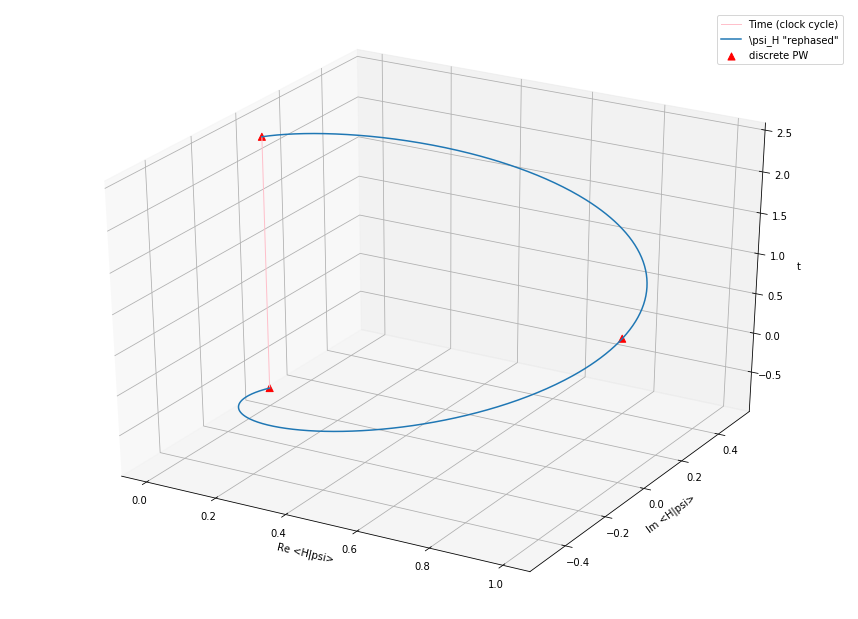
\includegraphics[width=\textwidth/2]{img/psi_H.png}
\caption[(from notebook)]{png}
\end{figure}

\begin{lstlisting}[language=Python]
mpl.rcParams['legend.fontsize'] = 10

fig = plt.figure(figsize=(15, 11))
ax = fig.gca(projection='3d')

# Prepare arrays x, y, z
# z is t
z = np.linspace(-np.pi/4, 3*np.pi/4, 500)

# Auto-broadcasting doesn't work as expected, therefore we explicitly
# map the z vector via `np.vectorize()`

# x is real part of psi[1] or Re(psi_V) as in psi = psi_H|H> + psi_V|V>
x = np.vectorize(lambda t: psi_fixed_1_re(t, -np.pi/4, [0, -1j], 0))(z) 
# y is imag part of psi[0] or Im(psi_H) as in psi = psi_H|H> + ps_V|V>
y = np.vectorize(lambda t: psi_fixed_1_im(t, -np.pi/4, [0, -1j], 0))(z) 

plt.plot([0, 0], [0, 0], [-np.pi/4, 3*np.pi/4], lw=1, c='pink', label='Time (clock cycle)')

ax.plot(x, y, z, label='psi_V "rephased"')

points_x = np.array([     0.0,     0.0,       0.0])
points_y = np.array([    -1.0,     0.0,      -1.0])
points_z = np.array([-np.pi/4, np.pi/4, 3*np.pi/4])
ax.scatter(points_x, points_y, points_z, marker='^', c='red', s=50, alpha=1.0, label='discrete PW')

plt.xlabel(s='Re <V|psi>')
plt.ylabel(s='Im <V|psi>')
ax.set_zlabel('t')

ax.legend()

plt.show()
\end{lstlisting}

\begin{figure}
\centering
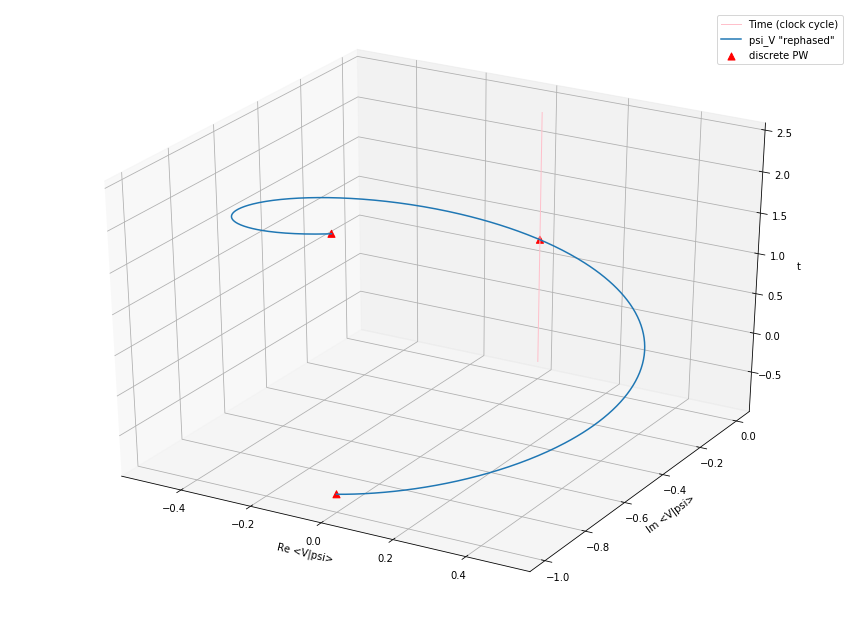
\includegraphics[width=\textwidth/2]{img/psi_V.png}
\caption[(from notebook)]{png}
\end{figure}

\graphicspath{{tex/appendix/nb/jupyter/detect/}}

\hypertarget{detector-model-kiukas-ruschhaupt-schmidt-werner}{%
\section{Detector model: Kiukas / Ruschhaupt / Schmidt /
Werner}\label{detector-model-kiukas-ruschhaupt-schmidt-werner}}

\begin{lstlisting}[language=Python]
from sympy import *
#from sympy.physics.matrices import mdft
from sympy.physics.quantum import TensorProduct
from sympy.functions.special.delta_functions import Heaviside
from sympy.physics.quantum.dagger import Dagger

from sympy.stats import ContinuousRV, variance, std

from sympy.plotting import plot, plot3d_parametric_line

import numpy as np
import matplotlib
import matplotlib.pyplot as plt

matplotlib.rcParams['text.usetex'] = True
#matplotlib.rcParams['text.latex.preamble'] = r'''
#    \usepackage{DejaVuSans}
#    \usepackage{xparse}
#    \usepackage{amsmath}
#    \usepackage{physics}
#'''
#matplotlib.rcParams['mathtext.fontset'] = 'dejavusans' 
#matplotlib.rcParams['mathtext.default'] = 'sf'
matplotlib.rcParams['figure.dpi'] = 140
# matplotlib.rcParams['figure.figsize'] = (8,8/sqrt(2))
matplotlib.rcParams['axes.labelsize'] = 16

# https://matplotlib.org/gallery/mplot3d/lines3d.html?highlight=parametric
# This import registers the 3D projection, but is otherwise unused.
from mpl_toolkits.mplot3d import Axes3D  # noqa: F401 unused import
\end{lstlisting}

\begin{lstlisting}[language=Python]
gamma = Symbol('gamma', real=True)
t = Symbol('t', real=True)
tprime = Symbol('t\'', real=True)
omega = Symbol('omega', real=True)
nu = Symbol('nu', real=True)
\end{lstlisting}

\begin{lstlisting}[language=Python]
def D(_gamma):
    return Rational(1, 2) * Matrix([
        [0, 0],
        [0, _gamma]
    ])
\end{lstlisting}

\begin{lstlisting}[language=Python]
H = Matrix ([
[0, 1] ,
[1, 0]
])
\end{lstlisting}

\begin{lstlisting}[language=Python]
init_printing ()
\end{lstlisting}

\begin{lstlisting}[language=Python]
H
\end{lstlisting}

\[\left[\begin{matrix}0 & 1\\1 & 0\end{matrix}\right]\]

\begin{lstlisting}[language=Python]
H.eigenvects()
\end{lstlisting}

\[\left [ \left ( -1, \quad 1, \quad \left [ \left[\begin{matrix}-1\\1\end{matrix}\right]\right ]\right ), \quad \left ( 1, \quad 1, \quad \left [ \left[\begin{matrix}1\\1\end{matrix}\right]\right ]\right )\right ]\]

It's manually seen that \(\langle H \rangle = 0\) and
\(\langle H^2 \rangle = 1\), therefore \(\sigma_{H} = 1\).

\begin{lstlisting}[language=Python]
def K(_gamma):
    return H - I*D(_gamma)
\end{lstlisting}

\begin{lstlisting}[language=Python]
K(2*sqrt(2))
\end{lstlisting}

\[\left[\begin{matrix}0 & 1\\1 & - \sqrt{2} i\end{matrix}\right]\]

\begin{lstlisting}[language=Python]
K(2*sqrt(2)).eigenvects()
\end{lstlisting}

\[\left [ \left ( - \frac{\sqrt{2}}{2} - \frac{\sqrt{2} i}{2}, \quad 1, \quad \left [ \left[\begin{matrix}- \frac{1}{\frac{\sqrt{2}}{2} + \frac{\sqrt{2} i}{2}}\\1\end{matrix}\right]\right ]\right ), \quad \left ( \frac{\sqrt{2}}{2} - \frac{\sqrt{2} i}{2}, \quad 1, \quad \left [ \left[\begin{matrix}- \frac{1}{- \frac{\sqrt{2}}{2} + \frac{\sqrt{2} i}{2}}\\1\end{matrix}\right]\right ]\right )\right ]\]

\begin{lstlisting}[language=Python]
def B(_gamma):
    return lambda t: exp(-I*K(_gamma)*t)
\end{lstlisting}

\begin{lstlisting}[language=Python]
def U():
    return lambda t: exp(-I*H*t)
\end{lstlisting}

\begin{lstlisting}[language=Python]
def non_unitary_psi(_t):
    return B(2*sqrt(2))(_t) * Matrix([1,0])
\end{lstlisting}

\begin{lstlisting}[language=Python]
def unitary_psi(_t):
    return U()(_t) * Matrix([1,0])
\end{lstlisting}

\begin{lstlisting}[language=Python]
non_unitary_psi(t)
\end{lstlisting}

\begin{equation}\label{eq:sympy:non-unitary-evol}
    \left[\begin{matrix}\frac{\sqrt{2} i t e^{- \frac{\sqrt{2} t}{2} - \frac{\sqrt{2} i t}{2}}}{2 \left(\frac{\sqrt{2} t}{2} + \frac{\sqrt{2} i t}{2}\right)} - \frac{\sqrt{2} i t e^{- \frac{\sqrt{2} t}{2} + \frac{\sqrt{2} i t}{2}}}{2 \left(\frac{\sqrt{2} t}{2} - \frac{\sqrt{2} i t}{2}\right)}\\\frac{\sqrt{2} e^{- \frac{\sqrt{2} t}{2} - \frac{\sqrt{2} i t}{2}}}{2} - \frac{\sqrt{2} e^{- \frac{\sqrt{2} t}{2} + \frac{\sqrt{2} i t}{2}}}{2}\end{matrix}\right]
\end{equation}

New period

\begin{lstlisting}[language=Python]
2*pi / (sqrt(2)/2)
\end{lstlisting}

\[2 \sqrt{2} \pi\]

Components are either pure real or pure imaginary:

\begin{lstlisting}[language=Python]
plot(re(non_unitary_psi(t)[0]), (t, 0, 10),
     line_color='r', xlabel=r'$t$', ylabel=r'$\mathrm{Re}\left\langle 0 | \psi \right\rangle $')
\end{lstlisting}

\begin{figure}
\centering
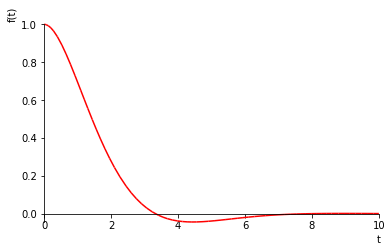
\includegraphics[width=0.6\linewidth]{output_20_0.png}
\caption[]{png}
\end{figure}

\begin{lstlisting}
<sympy.plotting.plot.Plot at 0x7fe25ffc9898>
\end{lstlisting}

\begin{lstlisting}[language=Python]
plot(im(non_unitary_psi(t)[1]), (t, 0, 10),
     line_color='b', xlabel=r'$t$', ylabel=r'$\mathrm{Im}\left\langle 1 | \psi \right\rangle $')
\end{lstlisting}

\begin{figure}
\centering
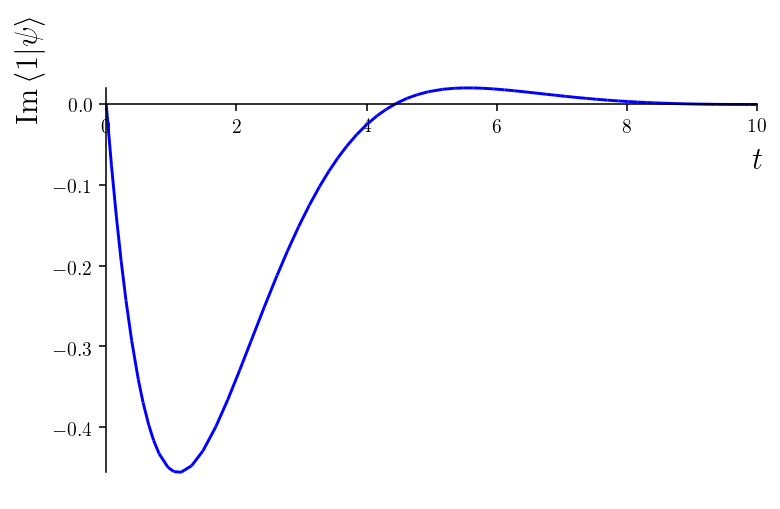
\includegraphics[width=0.6\linewidth]{output_21_0.png}
\caption[]{png}
\end{figure}

\begin{lstlisting}
<sympy.plotting.plot.Plot at 0x7fe25fec1780>
\end{lstlisting}

\begin{lstlisting}[language=Python]
# verify that our manual simplification is correct
#plot(-sqrt(2)*exp(-t*sqrt(2)/2)*sin(t*sqrt(2)/2), (t, 0, 10) )
\end{lstlisting}

\begin{lstlisting}[language=Python]
def lossy_norm(_t):
    psi = B(2*sqrt(2))(_t) * Matrix([1,0])
    return (abs(psi[0]**2) + abs(psi[1]**2))
\end{lstlisting}

\begin{lstlisting}[language=Python]
lossy_norm(t)
\end{lstlisting}

\[\left|{\left(\frac{\sqrt{2} e^{- \frac{\sqrt{2} t}{2} - \frac{\sqrt{2} i t}{2}}}{2} - \frac{\sqrt{2} e^{- \frac{\sqrt{2} t}{2} + \frac{\sqrt{2} i t}{2}}}{2}\right)^{2}}\right| + \left|{\left(\frac{\sqrt{2} i t e^{- \frac{\sqrt{2} t}{2} - \frac{\sqrt{2} i t}{2}}}{2 \left(\frac{\sqrt{2} t}{2} + \frac{\sqrt{2} i t}{2}\right)} - \frac{\sqrt{2} i t e^{- \frac{\sqrt{2} t}{2} + \frac{\sqrt{2} i t}{2}}}{2 \left(\frac{\sqrt{2} t}{2} - \frac{\sqrt{2} i t}{2}\right)}\right)^{2}}\right|\]

\begin{lstlisting}[language=Python]
non_unitary_psi_n = lambdify(t, non_unitary_psi(t), "numpy")
\end{lstlisting}

\begin{lstlisting}[language=Python]
_lossy_norm_n = lambdify(t, lossy_norm(t), "numpy")
def lossy_norm_n(__t):
    # prevent a warning, even if we know it's real
    return np.real(_lossy_norm_n(__t))
\end{lstlisting}

\begin{lstlisting}[language=Python]
lossy_norm_n
\end{lstlisting}

\begin{lstlisting}
<function __main__.lossy_norm_n(__t)>
\end{lstlisting}

\begin{lstlisting}[language=Python]
def non_unitary_psi_renorm_n(_t):
    return non_unitary_psi_n(_t) / np.sqrt(lossy_norm_n(_t))
\end{lstlisting}

\begin{lstlisting}[language=Python]
T = np.linspace(1e-16, 2*np.pi, 2000)
\end{lstlisting}

\begin{lstlisting}[language=Python]
fig = plt.figure(figsize=(8,8))
#fig = plt.figure()


ax = fig.gca(projection='3d')
ax.view_init(10,-45) # rotate 3d point of view

ax.plot(
    np.real(non_unitary_psi_n(T)[0][0]), np.imag(non_unitary_psi_n(T)[1][0]), T,
    linewidth=1.25
)

##ax.legend()

plt.xlabel(r'$\mathrm{Re}\left\langle 0 | \psi \right\rangle$ (pure real)', labelpad=8)
plt.ylabel(r'$\mathrm{Im}\left\langle 1 | \psi \right\rangle$ (pure imag)', labelpad=10)
ax.set_zlabel(r'$t$')
\end{lstlisting}

\begin{lstlisting}
Text(0.5, 0, '$t$')
\end{lstlisting}

\begin{figure}
\centering
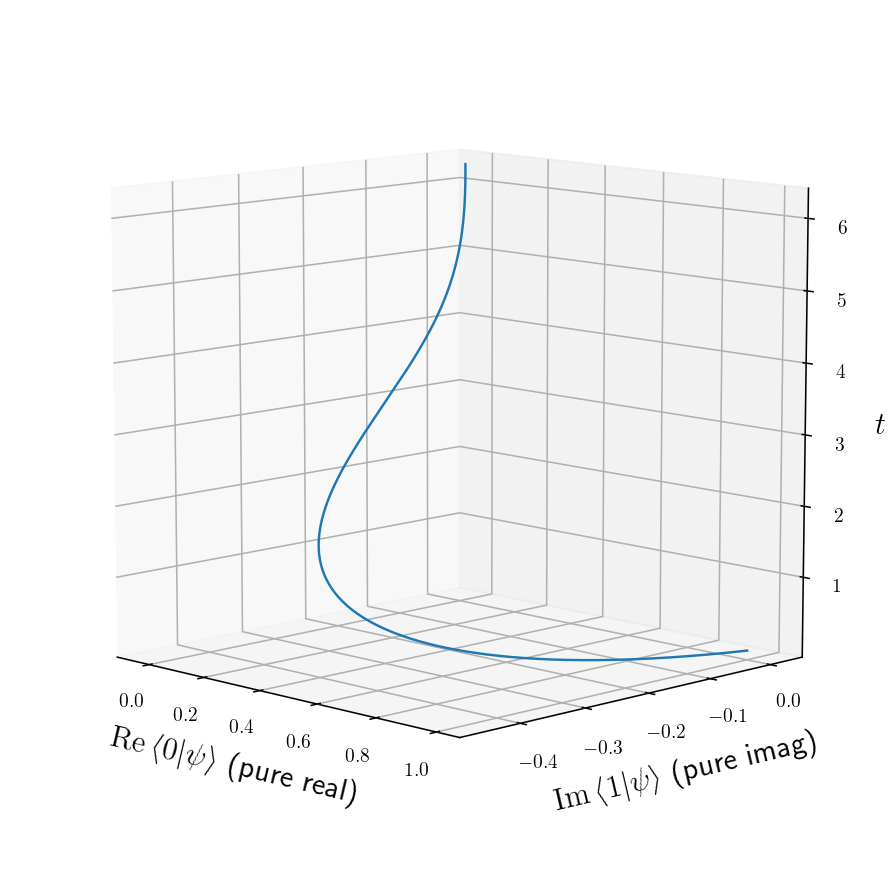
\includegraphics[width=0.6\linewidth]{output_30_1.png}
\caption[]{png}
\end{figure}

\begin{lstlisting}[language=Python]
plot(lossy_norm(t),(t, 0, 2*pi), line_color='g',
     ylabel=r'$\left|\psi\right|^2$', xlabel=r'$t$')
\end{lstlisting}

\begin{figure}
\centering
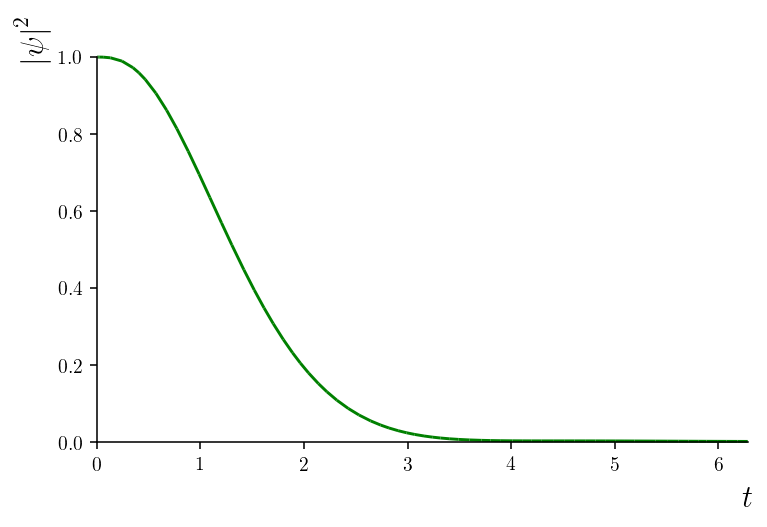
\includegraphics[width=0.6\linewidth]{output_31_0.png}
\caption[]{png}
\end{figure}

\begin{lstlisting}
<sympy.plotting.plot.Plot at 0x7fe25fe6a6a0>
\end{lstlisting}

\begin{lstlisting}[language=Python]
def prob_0_detect(t):
    return abs(non_unitary_psi(t)[0]**2) / lossy_norm(t)
\end{lstlisting}

\begin{lstlisting}[language=Python]
def prob_1_detect(t):
    return abs(non_unitary_psi(t)[1]**2) / lossy_norm(t)
\end{lstlisting}

\begin{lstlisting}[language=Python]
plot(prob_0_detect(t),(t, 0, 2*pi), line_color='r')
\end{lstlisting}

\begin{figure}
\centering
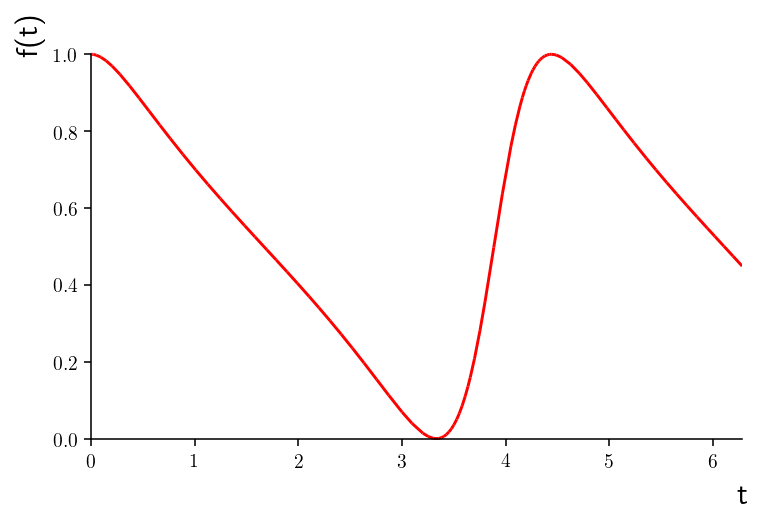
\includegraphics[width=0.6\linewidth]{output_34_0.png}
\caption[]{png}
\end{figure}

\begin{lstlisting}
<sympy.plotting.plot.Plot at 0x7fe25fddca20>
\end{lstlisting}

\begin{lstlisting}[language=Python]
plot(prob_1_detect(t),(t, -0, 2*pi), line_color='b')
\end{lstlisting}

\begin{figure}
\centering
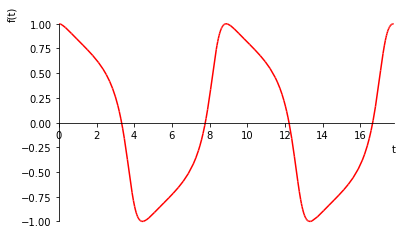
\includegraphics[width=0.6\linewidth]{output_35_0.png}
\caption[]{png}
\end{figure}

\begin{lstlisting}
<sympy.plotting.plot.Plot at 0x7fe25fd87ac8>
\end{lstlisting}

\begin{lstlisting}[language=Python]
plot(re(non_unitary_psi(t)[0])/sqrt(lossy_norm(t)), (t, 0, 2 * 2*sqrt(2)*pi), line_color='r')
\end{lstlisting}

\begin{figure}
\centering
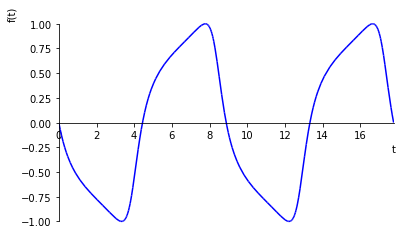
\includegraphics[width=0.6\linewidth]{output_36_0.png}
\caption[]{png}
\end{figure}

\begin{lstlisting}
<sympy.plotting.plot.Plot at 0x7fe25fd03128>
\end{lstlisting}

\begin{lstlisting}[language=Python]
plot(im(non_unitary_psi(t)[1])/sqrt(lossy_norm(t)), (t, 0, 2 * 2*sqrt(2)*pi), line_color='b')
\end{lstlisting}

\begin{figure}
\centering
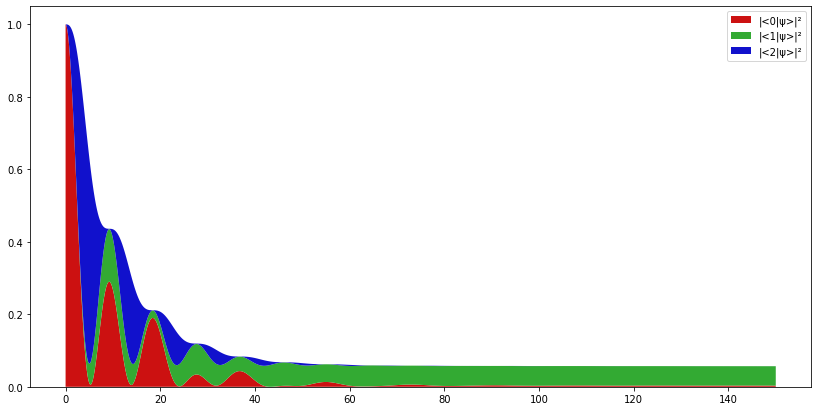
\includegraphics[width=0.6\linewidth]{output_37_0.png}
\caption[]{png}
\end{figure}

\begin{lstlisting}
<sympy.plotting.plot.Plot at 0x7fe25f98eeb8>
\end{lstlisting}

\begin{lstlisting}[language=Python]
plot(prob_0_detect(t) + prob_1_detect(t),(t, -0.25, 8*pi))
\end{lstlisting}

\begin{figure}
\centering
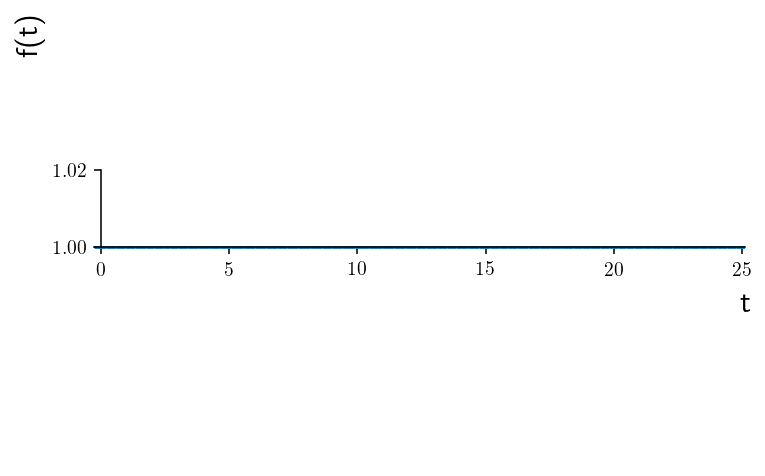
\includegraphics[width=0.6\linewidth]{output_38_0.png}
\caption[]{png}
\end{figure}

\begin{lstlisting}
<sympy.plotting.plot.Plot at 0x7fe261980c50>
\end{lstlisting}

\begin{lstlisting}[language=Python]
def prob_0_unitary(t):
    return abs(unitary_psi(t)[0]**2)
\end{lstlisting}

\begin{lstlisting}[language=Python]
def prob_1_unitary(t):
    return abs(unitary_psi(t)[1]**2)
\end{lstlisting}

\begin{lstlisting}[language=Python]
plot(prob_0_unitary(t),(t, -0.25, 8*pi), line_color='r')
\end{lstlisting}

\begin{figure}
\centering
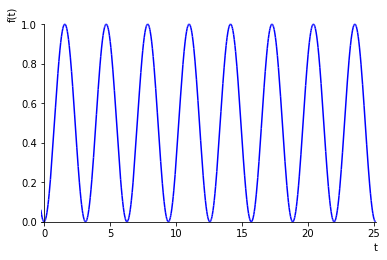
\includegraphics[width=0.6\linewidth]{output_41_0.png}
\caption[]{png}
\end{figure}

\begin{lstlisting}
<sympy.plotting.plot.Plot at 0x7fe261a495c0>
\end{lstlisting}

\begin{lstlisting}[language=Python]
plot(prob_1_unitary(t),(t, -0.25, 8*pi), line_color='b')
\end{lstlisting}

\begin{figure}
\centering
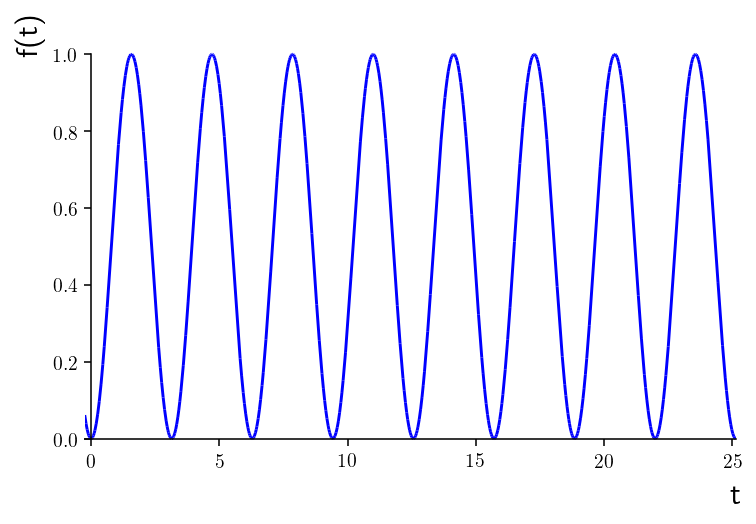
\includegraphics[width=0.6\linewidth]{output_42_0.png}
\caption[]{png}
\end{figure}

\begin{lstlisting}
<sympy.plotting.plot.Plot at 0x7fe25ff64710>
\end{lstlisting}

\begin{lstlisting}[language=Python]
lossy_norm_n(2)
\end{lstlisting}

\[0.19265133139031912\]

\begin{lstlisting}[language=Python]
X = np.linspace(1e-6, 2*np.pi, 1000)  # avoid singularity in t=0
\end{lstlisting}

\begin{lstlisting}[language=Python]
Y = lossy_norm_n(X)
\end{lstlisting}

\begin{lstlisting}[language=Python]
plt.xlabel('$t$')
plt.ylabel(r'$ - \mathrm{d}|\psi|^2 / \mathrm{d}t $')
plt.plot(X, -np.gradient(Y, X), 'g')
\end{lstlisting}

\begin{lstlisting}
[<matplotlib.lines.Line2D at 0x7fe25f7ddba8>]
\end{lstlisting}

\begin{figure}
\centering
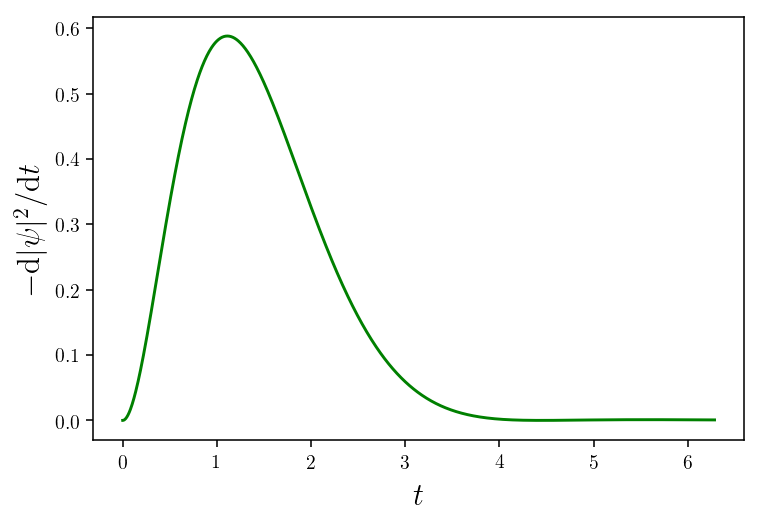
\includegraphics[width=0.6\linewidth]{output_46_1.png}
\caption[]{png}
\end{figure}

\begin{lstlisting}[language=Python]
# we have set gamma = 2*sqrt(2)
def hatpsi(_t):
    return \
        Heaviside(_t) * \
        2**(Rational(3,4)) * \
        Matrix([
            [0, 0],
            [0, 1]
        ]) * \
        non_unitary_psi(_t)
        
def hatpsi_n(_t):
    return \
        np.heaviside(_t, 0) * \
        2**(3/4) * \
        np.array([
            [0, 0],
            [0, 1]
        ]) * \
        non_unitary_psi_n(_t)
        
        
    
\end{lstlisting}

\begin{lstlisting}[language=Python]
hatpsi(t)
\end{lstlisting}

\begin{equation}\label{eq:sympy:hatpsi}
    \left[\begin{matrix}0\\2^{\frac{3}{4}} \left(\frac{\sqrt{2} e^{- \frac{\sqrt{2} t}{2} - \frac{\sqrt{2} i t}{2}}}{2} - \frac{\sqrt{2} e^{- \frac{\sqrt{2} t}{2} + \frac{\sqrt{2} i t}{2}}}{2}\right) \theta\left(t\right)\end{matrix}\right]
\end{equation}

\begin{lstlisting}[language=Python]
def hatpsisquarednorm(_t):
    return abs(hatpsi(_t)[0]**2) + abs(hatpsi(_t)[1]**2)

def hatpsisquarednorm_n(_t):
    return abs(hatpsi_n(_t)[0]**2) + abs(hatpsi_n(_t)[1]**2)
\end{lstlisting}

\begin{lstlisting}[language=Python]
hatpsisquarednorm(-1)
\end{lstlisting}

\[0\]

\begin{lstlisting}[language=Python]
plot(hatpsisquarednorm(t), (t, -1, 2*pi), line_color='g',
     ylabel=r'$ \left|\hspace{-.15em}\left|\hat{\psi}\right|\hspace{-.15em}\right|^2 $ =  $ - \mathrm{d}\left|\hspace{-0.15em}\left|\psi\right|\hspace{-0.15em}\right|^2 / \mathrm{d}t $',
     xlabel=r'$t$'
    )
\end{lstlisting}

\begin{figure}
\centering
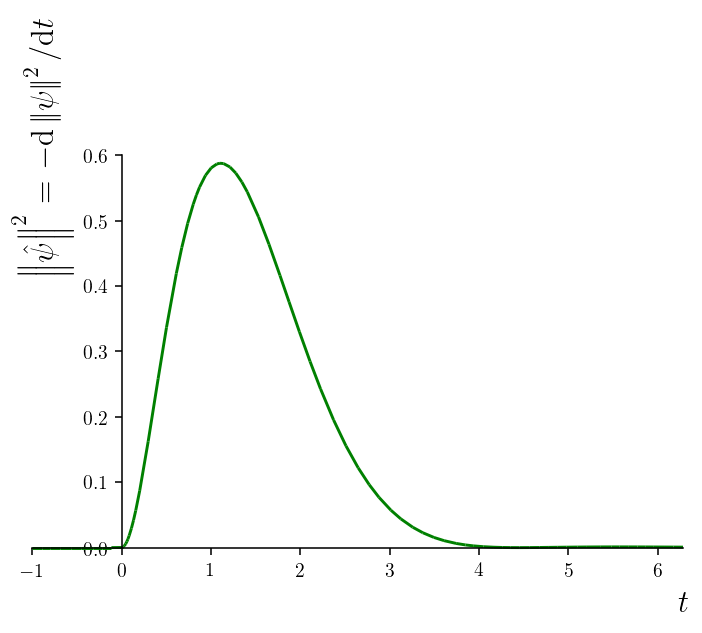
\includegraphics[width=0.6\linewidth]{output_51_0.png}
\caption[]{png}
\end{figure}

\begin{lstlisting}
<sympy.plotting.plot.Plot at 0x7fe25f7b05f8>
\end{lstlisting}

\begin{lstlisting}[language=Python]
#plot(prob_1_detect(t), hatpsisquarednorm(t), (t, -0.25, 8*pi))
\end{lstlisting}

\begin{lstlisting}[language=Python]
def prob_0_hatpsi(_t):
    return abs(hatpsi(_t)[0]**2) / (abs(hatpsi(_t)[0]**2) + abs(hatpsi(_t)[1]**2))
\end{lstlisting}

\begin{lstlisting}[language=Python]
def prob_1_hatpsi(_t):
    return abs(hatpsi(_t)[1]**2) / (abs(hatpsi(_t)[0]**2) + abs(hatpsi(_t)[1]**2))
\end{lstlisting}

\begin{lstlisting}[language=Python]
plot( abs(hatpsi(t)[1]**2), (t, -2, 2*pi), line_color='b')
\end{lstlisting}

\begin{figure}
\centering
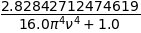
\includegraphics[width=0.6\linewidth]{output_55_0.png}
\caption[]{png}
\end{figure}

\begin{lstlisting}
<sympy.plotting.plot.Plot at 0x7fe25f7797f0>
\end{lstlisting}

\begin{lstlisting}[language=Python]
def fhatpsi1(_nu):
    return fourier_transform(hatpsi(t)[1], t, _nu)
\end{lstlisting}

\begin{lstlisting}[language=Python]
simplify(fhatpsi1(nu))
\end{lstlisting}

\[- \frac{2^{\frac{3}{4}} i}{- 4 \pi^{2} \nu^{2} + 2 \sqrt{2} i \pi \nu + 1}\]

\begin{lstlisting}[language=Python]
plot(abs(fhatpsi1(nu))**2, (nu, -1, 1), line_color='#bbbbbb')
\end{lstlisting}

\begin{figure}
\centering
\includegraphics[width=0.6\linewidth]{output_58_0.png}
\caption[]{png}
\end{figure}

\begin{lstlisting}
<sympy.plotting.plot.Plot at 0x7fe25f63ac18>
\end{lstlisting}

The above Fourier transform is defined in frequency ($\nu$) not angular
frequency ($\omega$), therefore needs rescaling.

\begin{lstlisting}[language=Python]
def fhatpsiomega(_omega):
    return fhatpsi1(_omega/(2*pi)) / sqrt((2*pi))
\end{lstlisting}

\begin{lstlisting}[language=Python]
fhatpsiomega(omega)
\end{lstlisting}

\begin{equation}\label{eq:fhatpsi1_omega}
    - \frac{\sqrt[4]{2} i}{\sqrt{\pi} \left(- \omega^{2} + \sqrt{2} i \omega + 1\right)}
\end{equation}

\begin{lstlisting}[language=Python]
abs(fhatpsiomega(omega))**2
\end{lstlisting}

\[- \frac{\sqrt{2}}{\pi \left(- \omega^{4} - 1\right)}\]

\begin{lstlisting}[language=Python]
integrate(abs(fhatpsiomega(omega))**2, (omega, -oo, +oo))
\end{lstlisting}

\[1\]

\begin{lstlisting}[language=Python]
plot(abs(fhatpsiomega(omega))**2, (omega, -2*pi, 2*pi), line_color='magenta', 
     xlabel=r'$\omega$', ylabel=r'$P(\omega)$')
\end{lstlisting}

\begin{figure}
\centering
\includegraphics[width=0.6\linewidth]{output_64_0.png}
\caption[]{png}
\end{figure}

\begin{lstlisting}
<sympy.plotting.plot.Plot at 0x7fe25dad3860>
\end{lstlisting}

\begin{lstlisting}[language=Python]
# graphical comparison with a normalized gaussian
sigma = 1.0
plot((1/(sqrt(2*pi)*sigma)) * exp(-omega**2/(2*(sigma)**2)), (omega, -2*pi, 2*pi), line_color='magenta')
\end{lstlisting}

\begin{figure}
\centering
\includegraphics[width=0.6\linewidth]{output_65_0.png}
\caption[]{png}
\end{figure}

\begin{lstlisting}
<sympy.plotting.plot.Plot at 0x7fe25dae10f0>
\end{lstlisting}

\hypertarget{discrete-page-wootters-model}{%
\subsection{(Discrete) Page-Wootters
model}\label{discrete-page-wootters-model}}

\begin{lstlisting}[language=Python]
from scipy.linalg import dft, norm, expm
from scipy import stats
\end{lstlisting}

\begin{lstlisting}[language=Python]
T = np.diag(np.arange(0,32)) * np.pi / 16
\end{lstlisting}

\begin{lstlisting}[language=Python]
# The NumPy Fourier matrix is the conjugate of Mathematica's one,
# hence the trailing .conj() 
F = dft(32, scale='sqrtn').conj()
\end{lstlisting}

\begin{lstlisting}[language=Python]
F_dagger = F.conj().T
\end{lstlisting}

\begin{lstlisting}[language=Python]
Omega = F @ T @ F_dagger * 16 / np.pi
\end{lstlisting}

\begin{lstlisting}[language=Python]
oeigenvalues, oeigenvectors = np.linalg.eig(Omega)
\end{lstlisting}

\begin{lstlisting}[language=Python]
np.round(oeigenvalues)
\end{lstlisting}

\begin{lstlisting}
array([-0.+0.j, 31.+0.j,  1.+0.j, 30.+0.j,  2.+0.j, 29.-0.j,  3.+0.j,
       28.-0.j,  4.-0.j, 27.-0.j,  5.-0.j, 26.+0.j,  6.-0.j, 25.+0.j,
        7.-0.j,  8.+0.j, 24.+0.j,  9.-0.j, 23.+0.j, 10.+0.j, 22.+0.j,
       11.+0.j, 21.-0.j, 12.+0.j, 13.-0.j, 20.-0.j, 14.-0.j, 15.-0.j,
       19.+0.j, 16.-0.j, 17.+0.j, 18.-0.j])
\end{lstlisting}

\begin{lstlisting}[language=Python]
H = np.array([
    [0, 1],
    [1, 0]
])
\end{lstlisting}

\begin{lstlisting}[language=Python]
D = np.array([
    [0, 0],
    [0, np.sqrt(2)]
])
\end{lstlisting}

\begin{lstlisting}[language=Python]
K = H - 1j*D
\end{lstlisting}

\begin{lstlisting}[language=Python]
K
\end{lstlisting}

\begin{lstlisting}
array([[0.+0.j        , 1.+0.j        ],
       [1.+0.j        , 0.-1.41421356j]])
\end{lstlisting}

\begin{lstlisting}[language=Python]
J = np.kron(Omega, np.eye(2)) + np.kron(np.eye(32), K)
\end{lstlisting}

\begin{lstlisting}[language=Python]
eigenvalues, eigenvectors = np.linalg.eig(J)
\end{lstlisting}

\begin{lstlisting}[language=Python]
EnergyCorrectionMatrices = np.zeros((64, 64, 64), np.complex)
for n in range(64):
    #EnergyCorrectionMatrices[n] = np.kron(
    #    expm(-1j*eigenvalues[n]*T),
    #    np.eye(2)
    #)
    EnergyCorrectionMatrices[n] = expm(-1j*eigenvalues[n]*np.kron(T, np.eye(2)))
# TODO: DRY
EnergyCorrectionMatricesT = np.zeros((64, 32, 32), np.complex)
for n in range(64):
    EnergyCorrectionMatricesT[n] = expm(-1j*eigenvalues[n]*T)
\end{lstlisting}

\begin{lstlisting}[language=Python]
def history_vector(eigenindex):
    # Needs matrix transposition ".T" (different convention as opposed to Mathematica)
    eigenvector = eigenvectors.T[eigenindex]
    return EnergyCorrectionMatrices[eigenindex] @ eigenvector

# "unflatten" the history_vector v into a a sequence of qubit component pairs
def reshape(v):
    return np.reshape(v, (-1,2))

# also make the first component real
def normalize_initial(v):
    vout = np.zeros(64, np.complex)
    # A phase factor to make it real
    vout = v * np.exp(-1j * np.angle(v[0]))
    # And a factor to normalize the initial state
    vout = vout / sqrt(
        np.abs(vout[0]**2) + np.abs(vout[1]**2)
    )
    return vout
\end{lstlisting}

\begin{lstlisting}[language=Python]
# Find the best linear combination to obtain |0> as initial state
def find_best():
    max_prob0 = 0
    max_prob0_i = 0
    max_prob0_j = 0
    for i in range(32):
        for j in range(32):
            qbi = reshape(history_vector(i))
            qbj = reshape(history_vector(j))
            qbit_hist = qbi + qbj
            prob0 = np.abs(qbit_hist[0][0]**2) / (
                np.abs(qbit_hist[0][0]**2) + np.abs(qbit_hist[0][1]**2)
            )
            if prob0 > max_prob0:
                max_prob0 = prob0
                max_prob0_i = i
                max_prob0_j = j
    print (max_prob0_i, max_prob0_j, max_prob0)
    return (max_prob0_i, max_prob0_j)
    
\end{lstlisting}

\begin{lstlisting}[language=Python]
# start with |0> as close as possible
i, j = find_best()
qbhistvec = normalize_initial(history_vector(i) + history_vector(j))
qbhist = reshape(qbhistvec) 
\end{lstlisting}

\begin{lstlisting}
1 21 1.0
\end{lstlisting}

\begin{lstlisting}[language=Python]
qbhist = qbhist.astype(complex)
\end{lstlisting}

Consitently with ``odinary QM'' findings, the component along
\textbar0\textgreater{} stays purely real, and the component along
\textbar1\textgreater{} stays purely imaginary.

\begin{lstlisting}[language=Python]
# Fill data for plotting
times = np.arange(0, 2*np.pi, np.pi/16)
norms = np.zeros(32)
probs0 = np.zeros(32)
probs1 = np.zeros(32)
# Components 0 are pure real, componets 1 are pure imag
real_parts0 = np.real(qbhist.T[0])
imag_parts1 = np.imag(qbhist.T[1])

for i in range(0, 32):
    norms[i] = (np.abs(qbhist[i][0]**2) + np.abs(qbhist[i][1]**2))
    probs0[i] = np.abs(qbhist[i][0]**2) / (
        np.abs(qbhist[i][0]**2) + np.abs(qbhist[i][1]**2) )
    probs1[i] = np.abs(qbhist[i][1]**2) / (
        np.abs(qbhist[i][0]**2) + np.abs(qbhist[i][1]**2) )
\end{lstlisting}

\begin{lstlisting}[language=Python]
plt.ylabel(r'$\mathrm{Re}{\;}_{T}\hspace{-.2em}\left\langle t | {}_{S}\hspace{-.2em}\left\langle 0 | \Psi \right\rangle\hspace{-.17em}\right\rangle $')
plt.xlabel(r'$t$')
plt.plot(times, real_parts0/norms[0], 'rs')
\end{lstlisting}

\begin{lstlisting}
[<matplotlib.lines.Line2D at 0x7fe25d36e438>]
\end{lstlisting}

\begin{figure}
\centering
\includegraphics[width=0.6\linewidth]{output_87_1.png}
\caption[]{png}
\end{figure}

\begin{lstlisting}[language=Python]
plt.ylabel(r'$\mathrm{Im}{\;}_{T}\hspace{-.2em}\left\langle t | {}_{S}\hspace{-.2em}\left\langle 1 | \Psi \right\rangle\hspace{-.17em}\right\rangle $')
plt.xlabel(r'$t$')
plt.plot(times, imag_parts1/norms[0], 'bs')
\end{lstlisting}

\begin{lstlisting}
[<matplotlib.lines.Line2D at 0x7fe25d27da90>]
\end{lstlisting}

\begin{figure}
\centering
\includegraphics[width=0.6\linewidth]{output_88_1.png}
\caption[]{png}
\end{figure}

\begin{lstlisting}[language=Python]
plt.plot(times, norms/norms[0], 'g^')
\end{lstlisting}

\begin{lstlisting}
[<matplotlib.lines.Line2D at 0x7ff538fd94e0>]
\end{lstlisting}

\begin{figure}
\centering
\includegraphics[width=0.6\linewidth]{output_89_1.png}
\caption[]{png}
\end{figure}

\begin{lstlisting}[language=Python]
plt.plot(times, probs0, 'rs')
\end{lstlisting}

\begin{lstlisting}
[<matplotlib.lines.Line2D at 0x7ff538f341d0>]
\end{lstlisting}

\begin{figure}
\centering
\includegraphics[width=0.6\linewidth]{output_90_1.png}
\caption[]{png}
\end{figure}

\begin{lstlisting}[language=Python]
plt.plot(times, probs1, 'bs')
\end{lstlisting}

\begin{lstlisting}
[<matplotlib.lines.Line2D at 0x7ff538f05f60>]
\end{lstlisting}

\begin{figure}
\centering
\includegraphics[width=0.6\linewidth]{output_91_1.png}
\caption[]{png}
\end{figure}

\begin{lstlisting}[language=Python]
fig = plt.figure(figsize=(7,7))

#ax = fig.gca(projection='3d')
ax = fig.add_subplot(111, projection='3d')
ax.view_init(10,-45) # rotate 3d point of view

ax.scatter(
    real_parts0, imag_parts1, times
)

##ax.legend()

plt.xlabel(r'$\mathrm{Re}\left\langle 0 | \psi \right\rangle$ (pure real)')
plt.ylabel(r'$\mathrm{Im}\left\langle 1 | \psi \right\rangle$ (pure imag)')
ax.set_zlabel('t')
\end{lstlisting}

\begin{lstlisting}
Text(0.5, 0, 't')
\end{lstlisting}

\begin{figure}
\centering
\includegraphics[width=0.6\linewidth]{output_92_1.png}
\caption[]{png}
\end{figure}

\hypertarget{detection-event}{%
\subsection{Detection event}\label{detection-event}}

\begin{lstlisting}[language=Python]
sqr2D = np.array([
    [0, 0],
    [0, 2**(3/4)]
])
\end{lstlisting}

\begin{lstlisting}[language=Python]
qbhistvec = qbhistvec.astype(np.complex)
\end{lstlisting}

\begin{lstlisting}[language=Python]
sqr2D = sqr2D.astype(np.complex)
\end{lstlisting}

\begin{lstlisting}[language=Python]
#prob_detect_v = np.kron(np.eye(32), sqr2D) @ qbhistvec
#
# More direct route, without going through histories
i, j = find_best()
prob_detect_v = \
    (np.kron(EnergyCorrectionMatricesT[i], sqr2D) @ eigenvectors.T[i]) + \
    (np.kron(EnergyCorrectionMatricesT[j], sqr2D) @ eigenvectors.T[j])

# normalize
prob_detect_v = prob_detect_v / norm(prob_detect_v)

\end{lstlisting}

\begin{lstlisting}
1 21 1.0
\end{lstlisting}

\begin{lstlisting}[language=Python]
prob_detect = np.zeros(32)
for t_idx in range(32):
    prob_detect[t_idx] = \
        np.abs(prob_detect_v[2*t_idx])**2 + np.abs(prob_detect_v[2*t_idx+1])**2
\end{lstlisting}

\begin{lstlisting}[language=Python]
plt.plot(times, prob_detect * 16 / np.pi, 'bs')
\end{lstlisting}

\begin{lstlisting}
[<matplotlib.lines.Line2D at 0x7ff538e5b550>]
\end{lstlisting}

\begin{figure}
\centering
\includegraphics[width=0.6\linewidth]{output_99_1.png}
\caption[]{png}
\end{figure}

\begin{lstlisting}[language=Python]
detect_fft = \
    np.kron(F, np.eye(2)) @ prob_detect_v
detect_fft = detect_fft / norm(detect_fft)
\end{lstlisting}

\begin{lstlisting}[language=Python]
prob_detect_fft = np.zeros(32)
for o in range(32):
    prob_detect_fft[o] = \
        np.abs(detect_fft[2*o]**2) + \
        np.abs(detect_fft[2*o + 1]**2) 
\end{lstlisting}

\begin{lstlisting}[language=Python]
# Arrays are "rolled" because the second half 
# of the spectrum is identified with
# negative frequencies.
plt.plot(range(-16, 16), np.roll(prob_detect_fft, -16), 'y^')
\end{lstlisting}

\begin{lstlisting}
[<matplotlib.lines.Line2D at 0x7ff538db5ac8>]
\end{lstlisting}

\begin{figure}
\centering
\includegraphics[width=0.6\linewidth]{output_102_1.png}
\caption[]{png}
\end{figure}

\begin{lstlisting}[language=Python]
S_t = stats.entropy(prob_detect)
\end{lstlisting}

\begin{lstlisting}[language=Python]
S_omega = stats.entropy(prob_detect_fft)
\end{lstlisting}

\begin{lstlisting}[language=Python]
S_t
\end{lstlisting}

\[2.6193337590390438\]

\begin{lstlisting}[language=Python]
S_omega
\end{lstlisting}

\[1.3471684169765332\]

\begin{lstlisting}[language=Python]
S_t * S_omega
\end{lstlisting}

\[3.528683713697821\]

\begin{lstlisting}[language=Python]
np.log(32)
\end{lstlisting}

\[3.4657359027997265\]

\begin{lstlisting}[language=Python]
(S_t * S_omega - np.log(32)) / np.log(32)
\end{lstlisting}

\[0.01816289892349938\]

Only 1.8\% more than the minumum per entropic uncertainty relation.

\hypertarget{use-scipy-routines-to-compute-sigmas}{%
\subsubsection{Use Scipy routines to compute
sigmas}\label{use-scipy-routines-to-compute-sigmas}}

\begin{lstlisting}[language=Python]

xk = range(-16,16)
pk = np.roll(prob_detect_fft, -16)
detect_fft_pdist = stats.rv_discrete(name='prob_detect_fft_minus16', values=(xk, pk))
\end{lstlisting}

\begin{lstlisting}[language=Python]
sigma_omega = detect_fft_pdist.std()
\end{lstlisting}

\begin{lstlisting}[language=Python]
xk = times
pk = prob_detect
detect_pdist = stats.rv_discrete(name='prob_detect', values=(xk, pk))
\end{lstlisting}

\begin{lstlisting}[language=Python]
sigma_t = detect_pdist.std()
\end{lstlisting}

\begin{lstlisting}[language=Python]
sigma_t * sigma_omega
\end{lstlisting}

\[0.7159703170687718\]

It's still quite a bit more than 0.5, i.e.~the minimum
uncertainty\ldots{}

But this is in fact consistent with the paper.

\hypertarget{detector-model-3-level-system}{%
\subsection{Detector model: 3-level
system}\label{detector-model-3-level-system}}

Three-level ``\(\Lambda\)'' system, of interest for * detector models
(decay into a metastable state), * STIRAP * EIT

\begin{lstlisting}[language=Python]
import numpy as np

import matplotlib
import matplotlib.pyplot as plt

from scipy.linalg import expm, norm

# matplotlib.rcParams['text.usetex'] = False

# https://matplotlib.org/gallery/mplot3d/lines3d.html?highlight=parametric
# This import registers the 3D projection, but is otherwise unused.
from mpl_toolkits.mplot3d import Axes3D  # noqa: F401 unused import
\end{lstlisting}

\begin{lstlisting}[language=Python]
matplotlib.rcParams['font.size'] = 14
matplotlib.rcParams['axes.labelsize'] = 16
matplotlib.rcParams['legend.fontsize'] = 16
matplotlib.rcParams['axes.labelpad']  = 14
\end{lstlisting}

\begin{lstlisting}[language=Python]
#matplotlib.rcParams
\end{lstlisting}

\begin{lstlisting}[language=Python]
from IPython.display import display, Latex #, Math
\end{lstlisting}

\begin{lstlisting}
%%javascript
    // do not generate scroll areas, expand figures instead
    IPython.OutputArea.auto_scroll_threshold = 9999
\end{lstlisting}

\begin{lstlisting}
<IPython.core.display.Javascript object>
\end{lstlisting}

\begin{lstlisting}[language=Python]
H = np.array([
    [-2,     0,      32],
    [0,      2,       8],
    [32,     8,       3]
], np.complex_) / 96
\end{lstlisting}

\begin{lstlisting}[language=Python]
def U(t):
    return expm(-1j*H*t)
\end{lstlisting}

\begin{lstlisting}[language=Python]
psi_0 = np.array([1, 0, 0], np.complex_)
\end{lstlisting}

\begin{lstlisting}[language=Python]
def unitary_psi(t):
    return U(t) @ psi_0
\end{lstlisting}

\begin{lstlisting}[language=Python]
def prob(t):
    probabilities = [0, 0, 0]
    for i in 0, 1, 2:
        probabilities[i] = norm(unitary_psi(t)[i])**2
    return probabilities
\end{lstlisting}

\begin{lstlisting}[language=Python]
TMIN, TMAX, TMAX_EXTENDED = 0, 40, 150
TMIN_N, TMAX_N = float(TMIN), float(TMAX)
\end{lstlisting}

\begin{lstlisting}[language=Python]
NPLOTPOINTS = 3200
\end{lstlisting}

\begin{lstlisting}[language=Python]
times = np.linspace(TMIN_N, TMAX_N, num=NPLOTPOINTS)
times_extended = np.linspace(TMIN_N, TMAX_EXTENDED, num=NPLOTPOINTS)
\end{lstlisting}

\begin{lstlisting}[language=Python]
probs = [None, None, None]
for i in 0, 1, 2:
    probs[i] = np.fromiter((prob(t)[i] for t in times), np.float)
#     fig, ax = plt.subplots(figsize=(12, 6*np.max(probs[i])))
#     ax.plot(times, probs[i])
#     plt.show()
\end{lstlisting}

\begin{lstlisting}[language=Python]
# Avoid *tiny* negative numbers, just out of numeric approximation, which will cause problems later,
# when their value is in fact juzt zero.
probs = np.round(probs, decimals=12)
\end{lstlisting}

\begin{lstlisting}[language=Python]
UNISYM = {
    'psi': u'\u03C8',
    '^2' : u'\u00B2'
}
PROB_LABELS        = ['', '', '']
PROB_AMP_LABELS    = ['', '', '']
PROB_AMP_LABELS_PW = ['', '', '']
                
for i in 0, 1, 2:
    PROB_AMP_LABELS[i] = '<' + str(i) + '|' + UNISYM['psi'] + '(t)' + '>'
    PROB_LABELS[i]     = '|' + PROB_AMP_LABELS[i] + '|' + UNISYM['^2']
    
    PROB_AMP_LABELS_PW[i] = '<t|\u2297<%d|\u03A8>>' % i
\end{lstlisting}

https://matplotlib.org/gallery/lines\_bars\_and\_markers/stackplot\_demo.html\#sphx-glr-gallery-lines-bars-and-markers-stackplot-demo-py

\begin{lstlisting}[language=Python]
prob_stack = np.vstack(probs)
\end{lstlisting}

\begin{lstlisting}[language=Python]
colors  =  ['#d44', '#4d4', '#44d']
colors  =  ['r', 'g', 'b']
hatches =  ['\\\\\\', '////////', '...']

linewidths =  [1, 1, 1]

labels     =  PROB_LABELS

fig, ax = plt.subplots(figsize=(12, 6))

stacks = ax.stackplot(times, (probs[0], probs[1], probs[2]))
ax.set_xlabel('t')

for stack, hatch, color, label, linewidth in zip(stacks, hatches, colors, labels, linewidths):
    stack.set_facecolor('w')
    stack.set_edgecolor(color)
    stack.set_label(label)
    stack.set_hatch(hatch)
    stack.set_linewidth(linewidth)
        
ax.plot(times, probs[0] + probs[1] + probs[2], c='m', label='||\u03C8(t)||\u00B2', linewidth=1.5)

desired_order   = [0, 3, 2, 1]
_handles, _labels = ax.get_legend_handles_labels()
handles         = [ _handles[i] for i in desired_order ]
labels          = [ _labels[i]  for i in desired_order ]
ax.legend(handles, labels, loc='center right', framealpha=1)

plt.savefig('_img/detect3.021/hermitian3color.pdf', bbox_inches='tight', pad_inches=0)
plt.show()
\end{lstlisting}

\begin{figure}[h!]
\centering
\includegraphics[width=0.66\linewidth]{tex/appendix/nb/jupyter/3lev/output_20_0.png}

\end{figure}

\begin{lstlisting}[language=Python]
rgbs = []
for i in range(NPLOTPOINTS):
    rgbs.append(
        (
            probs[0][i],
            probs[1][i],
            probs[2][i]
        )
    )
\end{lstlisting}

\begin{lstlisting}[language=Python]
fig, ax = plt.subplots(figsize=(12,6))
ax.set_xlabel('t')
ax.scatter(times, np.zeros(NPLOTPOINTS)-0.1,
            c=rgbs, marker='|', s=400)

# "virtual", don't really want to show, only for legend
_c = ['r', '#0a0', 'b']
for i in 0, 1, 2:
    ax.plot(
        times, probs[i],
        c=_c[i],
        linewidth=2,
    )
    
ax.legend(
    PROB_LABELS,
    loc='upper right'
)

plt.savefig('_img/detect3.021/hermitian3lines.pdf', bbox_inches='tight', pad_inches=0)
\end{lstlisting}

\begin{figure}[h!]
\centering
\includegraphics[width=0.66\linewidth]{tex/appendix/nb/jupyter/3lev/output_22_0.png}

\end{figure}

\begin{lstlisting}[language=Python]
unitary_psis = [np.zeros(NPLOTPOINTS)] * 3
for i in 0, 1, 2:
    unitary_psis[i] = np.fromiter( (unitary_psi(t)[i] for t in times), np.complex )
\end{lstlisting}


\begin{lstlisting}[language=Python]
# 3D parametric plot
for (vertical_angle,horizontal_angle,height,width,lloc,view) in (10,-70,12,12,'center left','side'), (80,-120,12,12,'right','top'):
    # fig = plt.figure(figsize=(w5dth, height), dpi=250)2
    fig = plt.figure(figsize=(width, height))

    ax = fig.gca(projection='3d')

    ax.view_init(vertical_angle, horizontal_angle) # rotate 3d point of view

    ax.set_xlabel('Re <0,1,2|\u03C8>')
    ax.set_ylabel('Im <0,1,2|\u03C8>')
    ax.set_zlabel('t')
    
    ax.scatter(
        np.zeros(NPLOTPOINTS, dtype=np.float),
        np.zeros(NPLOTPOINTS, dtype=np.float),
        times,
        c = rgbs,
        s = 24
    )
    for i in 0, 1, 2:
        ax.plot(
            np.real(unitary_psis[i]),
            np.imag(unitary_psis[i]),
            times,
            label = PROB_AMP_LABELS[i],
            #depthshade=False,
            c = _c[i]
        )
        ax.legend(loc=lloc)
    plt.savefig('_img/detect3.021/hermitianSpaceTime_%s.pdf' % view, bbox_inches=0, pad_inches=0)
\end{lstlisting}

\begin{figure}[h!]
\centering
\includegraphics[width=0.66\linewidth]{tex/appendix/nb/jupyter/3lev/output_25_0.png}

\end{figure}

\begin{figure}[h!]
\centering
\includegraphics[width=0.66\linewidth]{tex/appendix/nb/jupyter/3lev/output_25_1.png}

\end{figure}

\hypertarget{complex-potential-detection-by-absorption}{%
\subsection{Complex potential (detection by
absorption)}\label{complex-potential-detection-by-absorption}}

\begin{lstlisting}[language=Python]
H_n = H
\end{lstlisting}

\begin{lstlisting}[language=Python]
GAMMA = 0.1
\end{lstlisting}

\begin{lstlisting}[language=Python]
def D(_gamma=GAMMA):
    # no 1/2 factor, absorbed in the _gamma in the matrix here
    return np.array([
        [0, 0,      0],
        [0, 0,      0],
        [0, 0, _gamma]
    ], dtype=np.complex)
\end{lstlisting}

\begin{lstlisting}[language=Python]
D()
\end{lstlisting}

\begin{lstlisting}
array([[0. +0.j, 0. +0.j, 0. +0.j],
       [0. +0.j, 0. +0.j, 0. +0.j],
       [0. +0.j, 0. +0.j, 0.1+0.j]])
\end{lstlisting}

\begin{lstlisting}[language=Python]
def K(_gamma=GAMMA):
    return H_n - 1j*D(_gamma)
\end{lstlisting}

\begin{lstlisting}[language=Python]
K()
\end{lstlisting}

\begin{lstlisting}
array([[-0.02083333+0.j ,  0.        +0.j ,  0.33333333+0.j ],
       [ 0.        +0.j ,  0.02083333+0.j ,  0.08333333+0.j ],
       [ 0.33333333+0.j ,  0.08333333+0.j ,  0.03125   -0.1j]])
\end{lstlisting}

\begin{lstlisting}[language=Python]
def B(_t, _gamma=GAMMA):
    return expm(-1j*K(_gamma)*_t)
\end{lstlisting}

\begin{lstlisting}[language=Python]
B(0)
\end{lstlisting}

\begin{lstlisting}
array([[1.+0.j, 0.+0.j, 0.+0.j],
       [0.+0.j, 1.+0.j, 0.+0.j],
       [0.+0.j, 0.+0.j, 1.+0.j]])
\end{lstlisting}

\begin{lstlisting}[language=Python]
def non_unitary_psi(_t, _gamma=GAMMA):
    return B(_t, _gamma) @ psi_0
\end{lstlisting}

\begin{lstlisting}[language=Python]
evolution = np.zeros((3, NPLOTPOINTS), dtype=np.complex)
evolution_extended = np.zeros((3, NPLOTPOINTS), dtype=np.complex)

for i in 0, 1, 2:
    _iter = (non_unitary_psi(_t)[i] for _t in times)
    _iter_extended = (non_unitary_psi(_t)[i] for _t in times_extended)

    evolution[i] = np.fromiter(_iter, np.complex)
    evolution_extended[i] = np.fromiter(_iter_extended, np.complex)

_iter_norm = (norm(non_unitary_psi(_t)) for _t in times)
norms = np.fromiter(_iter_norm, np.float)

_iter_norm_extended = (norm(non_unitary_psi(_t)) for _t in times_extended)
norms_extended = np.fromiter(_iter_norm_extended, np.float)
\end{lstlisting}

\begin{lstlisting}[language=Python]
colors  =  ['#f66', '#6d6', '#88f']
colors  =  ['r', 'g', 'b']
hatches =  ['\\\\\\', '////////', '...']
labels     =  PROB_LABELS

fig, ax = plt.subplots(figsize=(12, 8))

ax.plot(times, np.ones(NPLOTPOINTS), c='grey', linestyle='dashed', label='Initial norm', linewidth=2.5)

ax.plot(times, norms**2, c='m', linewidth=1.5, label='||\u03C8(t)||\u00B2')

stacks = ax.stackplot(times, (
    np.abs(evolution[0])**2,
    np.abs(evolution[1])**2,
    np.abs(evolution[2])**2
))

ax.set_xlabel('t')

for stack, hatch, color, label in zip(stacks, hatches, colors, labels):
    stack.set_linewidth(.5)
    stack.set_facecolor('w')
    stack.set_edgecolor(color)
    stack.set_label(label)
    stack.set_hatch(hatch)
    
handles, labels = ax.get_legend_handles_labels()
desired_order = [0, 1, 4, 3, 2]
handles = [ handles[i] for i in desired_order ]
labels  = [  labels[i] for i in desired_order ]
ax.legend(handles, labels, loc='center')

plt.savefig('_img/detect3.021/loss3color.pdf', bbox_inches='tight', pad_inches=0)
plt.show()
\end{lstlisting}

\begin{figure}[h!]
\centering
\includegraphics[width=0.66\linewidth]{tex/appendix/nb/jupyter/3lev/output_37_0.png}

\end{figure}

\begin{lstlisting}[language=Python]
# loss of normalization, or integral of antiderivative...
bayesian_denominator_nonpw = 1 - norm(evolution.T[NPLOTPOINTS-1])**2  # TODO! explain/replace
\end{lstlisting}

\begin{lstlisting}[language=Python]
fig, ax = plt.subplots(figsize=(12, 8))
ax.set_xlabel('t')
ax.set_ylabel('Detection probability density  =  - d||\u03C8(t)||\u00B2 / dt')
ax.plot(times, -np.gradient(norms**2, times), c='y', linewidth=3)
plt.savefig('_img/detect3.021/loss.pdf', bbox_inches='tight', pad_inches=0)
\end{lstlisting}

\begin{figure}[h!]
\centering
\includegraphics[width=0.66\linewidth]{tex/appendix/nb/jupyter/3lev/output_39_0.png}

\end{figure}

\begin{lstlisting}[language=Python]
labels = PROB_LABELS

colors  =  ['r', 'g', '#ccf']
hatches =  ['\\\\\\\\', '///////', '.....']

fig, ax = plt.subplots(figsize=(14, 7))

ax.set_xlabel('t')

ax.plot(times_extended, np.ones(NPLOTPOINTS), c='grey', linestyle='dashed', label='Initial norm')

ax.plot(times_extended, norms_extended**2, c='m', linewidth=1, label='||\u03C8(t)||\u00B2')

stacks = ax.stackplot(times_extended, (
    np.abs(evolution_extended[0])**2,
    np.abs(evolution_extended[1])**2,
    np.abs(evolution_extended[2])**2
))

for stack, hatch, color, label in zip(stacks, hatches, colors, labels):
    stack.set_linewidth(1.25)
    stack.set_facecolor('w')
    stack.set_edgecolor(color)
    stack.set_label(label)
    stack.set_hatch(hatch)

handles, labels = ax.get_legend_handles_labels()
desired_order = [0, 1, 4, 3, 2]
handles = [ handles[i] for i in desired_order ]
labels  = [  labels[i] for i in desired_order ]
ax.legend(handles, labels, loc='center')

plt.savefig('_img/detect3.021/loss3color_ext.pdf', bbox_inches='tight', pad_inches=0)
plt.show()
\end{lstlisting}

\begin{figure}[h!]
\centering
\includegraphics[width=0.66\linewidth]{tex/appendix/nb/jupyter/3lev/output_40_0.png}

\end{figure}

\hypertarget{asymptotic-fidelity-for-1}{%
\subsubsection*{``Asymptotic'' fidelity for $\ket{1}$}\label{asymptotic-fidelity-for-1}}

\begin{lstlisting}[language=Python]
times_extended[-1]
\end{lstlisting}

\begin{lstlisting}
150.0
\end{lstlisting}

\begin{lstlisting}[language=Python]
norms_extended[-1]**2
\end{lstlisting}

\begin{lstlisting}
0.05684539507975811
\end{lstlisting}

\begin{lstlisting}[language=Python]
(np.abs(evolution_extended[1])**2)[-1] / norms_extended[-1]**2
\end{lstlisting}

\begin{lstlisting}
0.9414855990054901
\end{lstlisting}

\hypertarget{detection-probability}{%
\subsubsection{Detection probability}\label{detection-probability}}

\begin{lstlisting}[language=Python]
_detection_prob = -np.gradient(norms_extended**2, times_extended)
fig, ax = plt.subplots(figsize=(14, 7))
ax.set_xlabel('t')
ax.set_ylabel('Detection probability density  =  - d||\u03C8(t)||\u00B2 / dt')
ax.plot(times_extended, _detection_prob, c='y', linewidth=3)
plt.savefig('_img/detect3.021/loss_ext.pdf', bbox_inches='tight', pad_inches=0)
\end{lstlisting}

\begin{figure}[h!]
\centering
\includegraphics[width=0.66\linewidth]{tex/appendix/nb/jupyter/3lev/output_46_0.png}

\end{figure}

\hypertarget{d}{%
\paragraph{``3D''}\label{d}}

\begin{lstlisting}[language=Python]
# 3D parametric plot

for (vertical_angle,horizontal_angle,height,width,lloc,view) in (15,-80,15,15,'center left','side'), (90, -80, 15, 15,'center left','top'):
    fig = plt.figure(figsize=(width, height))

    ax = fig.gca(projection='3d')

    ax.view_init(vertical_angle, horizontal_angle) # rotate 3d point of view

    ax.set_xlabel('Re <0,1,2|\u03C8>')
    ax.set_ylabel('Im <0,1,2|\u03C8>')
    ax.set_zlabel('t')
    
    ax.scatter(
        np.zeros(NPLOTPOINTS, dtype=np.float),
        np.zeros(NPLOTPOINTS, dtype=np.float),
        times,
    
        c = np.array([
            np.abs(evolution[0])**2,
            np.abs(evolution[1])**2,
            np.abs(evolution[2])**2
        ]).T,
        s = 24,
        marker='o'
    )
    _c = ['r', 'g', 'b']
        
    for i in 0, 1, 2:
        ax.plot(
            np.real(evolution[i]),
            np.imag(evolution[i]),
            times,
            #depthshade=False,
            c = _c[i],
            linewidth=2,
            label = PROB_AMP_LABELS[i]
        )
        ax.legend(loc=lloc)
    plt.savefig('_img/detect3.021/NonHermitianSpaceTime_%s.pdf' % view, bbox_inches='tight', pad_inches=0)
\end{lstlisting}

\begin{figure}[h!]
\centering
\includegraphics[width=0.66\linewidth]{tex/appendix/nb/jupyter/3lev/output_48_0.png}
\end{figure}

\begin{figure}[h!]
\centering
\includegraphics[width=0.66\linewidth]{tex/appendix/nb/jupyter/3lev/output_48_1.png}

\end{figure}

\hypertarget{page-wootters}{%
\subsection{Page-Wootters}\label{appendix:jupyter:3lev:page-wootters}}

\begin{lstlisting}[language=Python]
from scipy.linalg import dft, norm, expm, det, inv
\end{lstlisting}

\begin{lstlisting}[language=Python]
# Dimension of the system, or the spatial/"ordinary" Hilbert space
NS = 3
# Number of levels of the clock aka dimension of Time Hilbert space
NT = 60
# "Period"
DT = TMAX_N  # assume we start with time 0

T = DT * np.diag(np.arange(NT)) / NT
\end{lstlisting}

\begin{lstlisting}[language=Python]
\end{lstlisting}

\begin{lstlisting}[language=Python]
F = dft(NT, scale='sqrtn')
F_dagger = F.conj().T
\end{lstlisting}

\begin{lstlisting}[language=Python]
Omega = F_dagger @ T @ F * 2*np.pi * NT / DT**2
\end{lstlisting}

\begin{lstlisting}[language=Python]
J = np.kron(Omega, np.eye(3)) + np.kron(np.eye(NT), K())
\end{lstlisting}

\begin{lstlisting}[language=Python]
eigenvalues, eigenvectors = np.linalg.eig(J)
\end{lstlisting}

\begin{lstlisting}[language=Python]
eigenvectors = eigenvectors.T
\end{lstlisting}

\begin{lstlisting}[language=Python]
eigenvectors_normalized_in_S = np.empty((NT*NS, NT*NS), dtype=complex)

for i in range(NT*NS):
    eigenvectors_normalized_in_S[i] = eigenvectors[i] / norm(eigenvectors[i][:3])
\end{lstlisting}

\begin{lstlisting}[language=Python]
histories = np.empty((NT*NS, NT*NS), dtype=complex)

for i in range(NT*NS):
    histories[i] = \
        expm(np.kron( -1j*T*eigenvalues[i], np.eye(NS) )) @ \
        eigenvectors_normalized_in_S[i]
\end{lstlisting}

\begin{lstlisting}[language=Python]
# Only implemented for NS=3
def find_linear_independent_initial(eigenvectors=eigenvectors_normalized_in_S):
    best_i, best_j, best_k = -1, -1, -1
    best_det = 0
    best_states = np.array([
        [0, 0, 0],
        [0, 0, 0],
        [0, 0, 0]
    ])
    for i in range(NT*NS):
        for j in range(i, NT*NS):
            for k in range(j, NT*NS):
                # this normalization is not necessary if default
                # eigenvectors=eigenvectors_normalized_in_S
                # is given
                si = eigenvectors[i][:3]
                si = si / norm(si)
                sj = eigenvectors[j][:3]
                sj = sj / norm(sj)
                sk = eigenvectors[k][:3]
                sk = sk / norm(sk)
                states = np.array([
                    si,
                    sj,
                    sk
                ])
                _det = det(states)
                if abs(abs(_det)-1.0) < abs(abs(best_det) - 1.0):
                    best_det = _det
                    best_i, best_j, best_k = i, j, k
                    best_states = states
                if abs(abs(_det)-1.0) == 0:
                    return best_i, best_j, best_k, best_det
        percent = int(100 * (i + 1) / (NT*NS))
        print(
            str(percent) + '% scanned' + "\tabs(best_det) = " + str(abs(best_det)),
            end="\r", flush=True)
        
    return best_i, best_j, best_k, best_det

\end{lstlisting}

\begin{lstlisting}[language=Python]
best_i, best_j, best_k, best_det = find_linear_independent_initial()
\end{lstlisting}

\begin{lstlisting}
100% scanned    abs(best_det) = 0.9893579012772128
\end{lstlisting}

\begin{lstlisting}[language=Python]
states = np.array([
    histories[best_i][:NS],
    histories[best_j][:NS],
    histories[best_k][:NS]
])
#assert(np.round(abs(det(states)), decimals=2) == 1.0)
# Find what linear combination would bring to the desired initial state psi_0_n
coeffs = inv(states.T) @ psi_0
\end{lstlisting}

\begin{lstlisting}[language=Python]
history = coeffs.dot(np.array([
    histories[best_i],
    histories[best_j],
    histories[best_k]
]))
\end{lstlisting}

\begin{lstlisting}[language=Python]
# 3D parametric plot

times_discrete = np.diag(T)

psi = history.reshape((-1,NS)).T

for (vertical_angle,horizontal_angle,height,width,lloc,view) in ((10,-120,15,25,'center right','side'), (80,-100,15,25,'center right','top')):
    fig = plt.figure(figsize=(width, height))


    ax = fig.gca(projection='3d')

    ax.view_init(vertical_angle, horizontal_angle) # rotate 3d point of view

    ax.set_xlabel('Re <t|\u2297<0,1,2|\u03A8>>')
    ax.set_ylabel('Im <t|\u2297<0,1,2|\u03A8>>')
    ax.set_zlabel('t')
    
    ax.scatter(
        np.zeros(NT, dtype=np.float),
        np.zeros(NT, dtype=np.float),
        times_discrete,
    
        c = np.round((abs(psi.T)**2), 8), # rounding, to avoid number instability causing out-of-range rgb vals
        s = 75,
        marker='o'
    )
    _c = ['r', 'g', 'b']

    for i in range(NS):
        ax.scatter(
            np.real(
                psi[i]
            ),
            np.imag(
                psi[i]
            ),
            times_discrete,

            marker = 's',
            #depthshade=False,
            #s = abs(_psi[i]**2)*60,
            s = 60,
            edgecolor = _c[i],
            facecolor = (0, 0, 0, 0),
            linewidth = 1,

            label = PROB_AMP_LABELS_PW[i]
        )
    ax.legend(loc=lloc)
    plt.savefig('_img/detect3.021/PWSpaceTime_%s.pdf' % view, bbox_inches='tight', pad_inches=0)
\end{lstlisting}

\begin{figure}[h!]
\centering
\includegraphics[width=0.66\linewidth]{tex/appendix/nb/jupyter/3lev/output_64_0.png}

\end{figure}

\begin{figure}[h!]
\centering
\includegraphics[width=0.66\linewidth]{tex/appendix/nb/jupyter/3lev/output_64_1.png}

\end{figure}

\begin{lstlisting}[language=Python]
norm(psi)**2
\end{lstlisting}

\begin{lstlisting}
18.550562258122728
\end{lstlisting}

\begin{lstlisting}[language=Python]
norm(psi)
\end{lstlisting}

\begin{lstlisting}
4.307036366008851
\end{lstlisting}

\hypertarget{overlapping-pw-and-qm-continuous}{%
\subsubsection{Overlapping PW and QM
continuous}\label{overlapping-pw-and-qm-continuous}}

\begin{lstlisting}[language=Python]
# 3D parametric plot

times_discrete = np.diag(T)

psi = history.reshape((-1,NS)).T

for (vertical_angle,horizontal_angle,height,width,view) in (15,-80,15,15,'side'), (90,-80,15,15,'top'):
    # fig = plt.figure(figsize=(width, height), dpi=300)
    fig = plt.figure(figsize=(width, height))

    ax = fig.gca(projection='3d')

    ax.view_init(vertical_angle, horizontal_angle) # rotate 3d point of view

    ax.set_xlabel('Re')
    ax.set_ylabel('Im')
    ax.set_zlabel('t')
    
    ax.scatter(
        np.zeros(NT, dtype=np.float),
        np.zeros(NT, dtype=np.float),
        times_discrete,
    
        c = np.round((abs(psi.T)**2), 8), # rounding, to prevent numeric instability from causing out-of-range RGB values
        s = 75,
        marker='o'
    )
    _c = ['r', 'g', 'b']
    for i in range(NS):
        ax.scatter(
            np.real(
                psi[i]
            ),
            np.imag(
                psi[i]
            ),
            times_discrete,

            marker = 's',
            #depthshade=False,
            #s = abs(_psi[i]**2)*60,
            s = 80,
            edgecolor = _c[i],
            facecolor = (0, 0, 0, 0),
            linewidth = 0.8,
            label = PROB_AMP_LABELS_PW[i]
        )
        
    # QM continuous
    for i in 0, 1, 2:
        ax.plot(
            np.real(evolution[i]),
            np.imag(evolution[i]),
            times,
            #depthshade=False,
            c = _c[i],
            linewidth=1.5,
            label = PROB_AMP_LABELS[i]
        )
    ax.legend(loc='center left')
    plt.savefig('_img/detect3.021/PWSpaceTimeFit_%s.pdf' % view, bbox_inches='tight', pad_inches=0)
\end{lstlisting}

\begin{figure}[h!]
\centering
\includegraphics[width=0.66\linewidth]{tex/appendix/nb/jupyter/3lev/output_68_0.png}

\end{figure}

\begin{figure}[h!]
\centering
\includegraphics[width=0.66\linewidth]{tex/appendix/nb/jupyter/3lev/output_68_1.png}

\end{figure}

\hypertarget{toa-prob-as-in-macconesacha-arxiv1810.12869}{%
\subsection{TOA prob as in Maccone/Sacha
arXiv:1810.12869}\label{toa-prob-as-in-macconesacha-arxiv1810.12869}}

\emph{Adapted from \(\S\) ``Time of arbitrary event''.}


\begin{lstlisting}[language=Python]
def t_eigenstate(n):
    v = np.zeros(NT, dtype=np.complex)
    v[n] = 1
    return v
\end{lstlisting}

\begin{lstlisting}[language=Python]
arrived_state = np.array([0, 0, 1])
\end{lstlisting}

\begin{lstlisting}[language=Python]
def tn_ox_arrived(n):
    return np.kron(t_eigenstate(n), arrived_state)
\end{lstlisting}

\begin{lstlisting}[language=Python]
history_normalized = history / norm(history)  ## normalized in H_T \otimes H_S
\end{lstlisting}

\begin{lstlisting}[language=Python]
def joint_prob(n):
    return np.abs(tn_ox_arrived(n) @ history_normalized)**2
\end{lstlisting}

\begin{lstlisting}[language=Python]
X = np.arange(NT)

iterable = (joint_prob(n) for n in X)
Y = np.fromiter(iterable, float)
\end{lstlisting}

\begin{lstlisting}[language=Python]
dT  = DT / (NT)
\end{lstlisting}

\begin{lstlisting}[language=Python]
# A "time bin"
X = X * dT # real time
Y = Y / dT # probability _density_
\end{lstlisting}

\begin{lstlisting}[language=Python]
bayes_denominator = np.sum(Y * dT)
Y = Y / bayes_denominator
\end{lstlisting}

\begin{lstlisting}[language=Python]
# fig, ax = plt.subplots(figsize=(12, 8), dpi=300)
fig, ax = plt.subplots(figsize=(12, 8))
ax.set_xlabel('t')
ax.set_ylabel('Detection probability density')
ax.plot(X, Y, 'bs', label='Page-Wootters (Maccone / Sacha -- Bayesian / conditional)')
ax.plot(times, -np.gradient(norms**2, times) / bayesian_denominator_nonpw,
        c='y', linewidth=2, label='Detector model (normalization loss)')
ax.legend()
plt.savefig('_img/detect3.021/conditionalProbFit.pdf', bbox_inches='tight', pad_inches=0)
plt.show()
\end{lstlisting}

\begin{figure}[h!]
\centering
\includegraphics[width=0.66\linewidth]{tex/appendix/nb/jupyter/3lev/output_79_0.png}

\end{figure}

\begin{lstlisting}[language=Python]
nonpw_probs = -np.gradient(norms**2, times) / bayesian_denominator_nonpw
\end{lstlisting}

\begin{lstlisting}[language=Python]
np.sum(nonpw_probs*times[1])
\end{lstlisting}

\begin{lstlisting}
1.0000197507624184
\end{lstlisting}

\begin{lstlisting}[language=Python]
np.sum(Y*dT)
\end{lstlisting}

\begin{lstlisting}
1.0
\end{lstlisting}

\begin{lstlisting}[language=Python]
\end{lstlisting}


\chapter[Mathematica notebooks]{Mathematica notebooks\footnote{
  Ref.: \cite{Wolfram}.
}}
\section*{Preliminary note}

Here we just report the necessary Mathematica commands
and suppress some intermediate outputs,
using \verb#TeXForm[]# otherwise,
in lack of a viable export functionality
available for whole notebooks.

Minimal edit on expressions has been performed for formatting purposes only.
\section[
  \texttt{NN}-level clock $+$ $2$-level system
]{%
  Page--Wootters model: \texttt{NN}-level clock $+$ $2$-level system\footnote{
    Here the symbol \texttt{NN} is used instead of \texttt{N} to avoid confusion with
    Mathematica's \emph{function} \texttt{N[]} which
    is used to convert symbolic expressions to their numerical value.
  }
}
\label{appendix:n-level}

\begin{Verbatim}
NN := 32
\end{Verbatim}

\begin{Verbatim}
T := DiagonalMatrix[Range[0,NN-1]] * \[Pi] / 16
\end{Verbatim}

\begin{Verbatim}
F := FourierMatrix[NN]
\end{Verbatim}

For simplicity, $\hbar = \omega = 1$

\begin{Verbatim}
\[CapitalOmega] := F.T.F\[ConjugateTranspose]  * 16 / \[Pi]
\end{Verbatim}

Hamiltonian in "ordinary" space
\begin{Verbatim}
Hs := \[ImaginaryI]{{0, 1}, {-1, 0}}
\end{Verbatim}
\begin{Verbatim}
MatrixForm[Hs]
\end{Verbatim}
\[
  \left(
    \begin{array}{cc}
     0 & i \\
     -i & 0 \\
    \end{array}
    \right)
\]

Matrix representation of \cite[eq. 1]{Lloyd:Time}.
We turn it into numeric (\verb!N[ ]!) as treating  it symbolically onwards would be unfeasible:
\begin{Verbatim}
J := N[KroneckerProduct[\[CapitalOmega],IdentityMatrix[2]] + KroneckerProduct[IdentityMatrix[NN],Hs]]
\end{Verbatim}
\begin{Verbatim}
Chop[Eigenvalues[J]]

Out[ ] = {32., 31., 30., 30., 29., 29., 28., 28., 27., 27., 26., 26., 25., 25., 24., 24., 23., 23., 22., 22., 21., 21., 20., 20., 19., 19., 18., 18., 17., 17., 16., 16., 15., 15., 14., 14., 13., 13., 12., 12., 11., 11., 10., 10., 9., 9., 8., 8., 7., 7., 6., 6., 5., 5., 4., 4., 3., 3., 2., 2., 1., 1., -1., 0}
\end{Verbatim}
\begin{Verbatim}
Eigenvalues[J][[40]]

Out[ ] = 12.

Eigenvalues[J][[41]]

Out[ ] = 11.

chosenEigenvector := Eigenvectors[J][[ 40]]

chosenEigenvectorB := Eigenvectors[J][[41]]

Normalization := Sqrt[Abs[chosenEigenvector[[1]]^2] + Abs[chosenEigenvector[[2]]^2] ]

NormalizationB := Sqrt[Abs[chosenEigenvectorB[[1]]^2] + Abs[chosenEigenvectorB[[2]]^2] ]

chosenEigenvectorNormalized  := chosenEigenvector / Normalization

chosenEigenvectorNormalizedB := chosenEigenvectorB / NormalizationB  

probability := Abs[chosenEigenvectorNormalized ^2]

probabilityB := Abs[chosenEigenvectorNormalizedB^2]

ListPlot[probability,
  GridLines ->{Range[0,NN*2, 2], Range[0, 1, 0.1]},
  AxesLabel->{n, "P(0), P(1)"},
  LabelStyle->Directive[16],
  PlotMarkers->{Automatic, 16},
  ImageSize->1024
]
\end{Verbatim}
\begin{figure}[!h]
  \centering
  \includegraphics[width=.75\textwidth]{img/N32.png}
  \caption[]{png}{P-W ``evolution'' for $\hat{\mathbb{J}}$ eigenvalue $=12$}
\end{figure}  
\begin{Verbatim}

ListPlot[probabilityB,
  GridLines ->{Range[0,NN*2, 2], Range[0, 1, 0.1]},
  AxesLabel->{n, "P(0), P(1)"},
  LabelStyle->Directive[16],
  PlotMarkers->{Automatic, 16},
  ImageSize->1024
]
\end{Verbatim}
\begin{figure}[!h]
  \centering
  \includegraphics[width=.75\textwidth]{img/N32-B.png}
  \caption[]{png}{P-W ``evolution'' for $\hat{\mathbb{J}}$ eigenvalue $=11$}
\end{figure}

\subsection{Consistency of PW with ordinary QM (discrete approximation)}

\begin{Verbatim}
psi0 :=  chosenEigenvectorNormalizedB[[{1,2}]]
\end{Verbatim}

\begin{Verbatim}
psi[t_] := MatrixExp[-I Hs t, psi0 ]
\end{Verbatim}

\begin{Verbatim}
Plot[(Abs[psi[t]]^2)[[1]],{t,0,2\[Pi]},
  AxesLabel->{t, "P(0)"},
  LabelStyle->Directive[16],
  ImageSize->900
]
\end{Verbatim}
\begin{figure}[!h]
  \centering
  \includegraphics[width=0.75\textwidth]{img/probB_0.png}
  \caption[]{png}{
    Schr{\"o}dinger evolution of
    $\qty|\braket{0}{\psi(t)}|^2$, $t \in (0, 2\pi) $
    picking the first two components of an eigenvector of $\hat{\mathbb{J}}$
    as the two components of $\psi_{t=0}$ in ordinary Hilbert space.
    Related eigenvalue of $\hat{\mathbb{J}}$ is $11$
  }
\end{figure}

\begin{Verbatim}
Plot[(Abs[psi[t]]^2)[[2]],{t,0,2\[Pi]},
  AxesLabel->{t, "P(1)"},
  LabelStyle->Directive[16],
  ImageSize->900
]
\end{Verbatim}
\begin{figure}[!h]
  \centering
  \includegraphics[width=0.75\textwidth]{img/probB_1.png}
  \caption[]{png}{
    Schr{\"o}dinger evolution of
    $\qty|\braket{1}{\psi(t)}|^2$, $t \in (0, 2\pi) $
    picking the first two components of an eigenvector of $\hat{\mathbb{J}}$
    as the two components of $\psi_{t=0}$ in ordinary Hilbert space.
    Related eigenvalue of $\hat{\mathbb{J}}$ is $11$
  }
\end{figure}

\subsubsection{Complex evolution of $\psi$ (not just $\qty|\psi|^2$)}

Please note index count is
$1, 2$ (cells above)
but refers, respectively, to computational base elements
$\ket{0}, \ket{1}$ in ordinary Hilbert space.
\begin{Verbatim}
re0psi[t_] := Simplify[Re[psi[t][[1]]], Assumptions->Element[t, Reals]]
im0psi[t_] := Simplify[Im[psi[t][[1]]], Assumptions->Element[t, Reals]]
re1psi[t_] := Simplify[Re[psi[t][[2]]], Assumptions->Element[t, Reals]]
im1psi[t_] := Simplify[Im[psi[t][[2]]], Assumptions->Element[t, Reals]]
\end{Verbatim}

\begin{Verbatim}
zAxis := ParametricPlot3D[{0,0,t}, {t,0,2\[Pi]}, PlotStyle->{Gray}]
psi0plot := ParametricPlot3D[{re0psi[t], im0psi[t], t}, {t, 0, 2\[Pi]}, PlotStyle->{Red} ]
psi1plot := ParametricPlot3D[{re1psi[t], im1psi[t], t}, {t, 0, 2\[Pi]}, PlotStyle->{Blue} ]
\end{Verbatim}

\begin{Verbatim}
Show[zAxis, psi0plot,psi1plot, ImageSize->Medium,
  AxesLabel -> {
    Style[Re["<0,1|\[Psi]>"], Bold],
    Style[Im["<0,1|\[Psi]>"], Bold],
    Style[t, Bold]
  }
]
\end{Verbatim}
\begin{figure}[!h]
  \centering
  \includegraphics[width=0.25\textwidth]{img/qubit-evo-schrod.png}
  \caption[]{png}{
    Schr{\"o}dinger full complex evolution of components
    $\braket{0}{\psi(t)}$ (red) and 
    $\braket{1}{\psi(t)}$ (blue) for
    $t \in (0, 2\pi) $. The initial state
    has been chosen as the first two components of an eigenstate of
    $\hat{\mathbb{J}}$, related to eigenvalue $= 11$.
  }
\end{figure}

\begin{Verbatim}
pi = N[\[Pi]]

3.14159
\end{Verbatim}

\begin{Verbatim}
rephased[k_] := chosenEigenvectorNormalizedB [[k]] * Exp[-\[ImaginaryI]*pi*11*(k-1)/NN]

rephased1[k_] := chosenEigenvectorNormalizedB [[k]] * Exp[-\[ImaginaryI]*pi*11*(k-2)/NN]

scatter[k_] := {Re[ rephased[k]], Im[ rephased[k]], pi*(k-1)/NN}

scatter1[k_] := {Re[ rephased1[k]], Im[ rephased1[k]], pi*(k-2)/NN}

scatterPoints = Map[scatter, Range[1,2*NN, 2]]

Out[ ] = {{0.891003,-0.00706481,0.}, {0.896671,-0.0925068,0.19635}, {0.86788,-0.174394,0.392699}, {0.805737,-0.249579,0.589049}, {0.71263,-0.315173,0.785398}, {0.592137,-0.368655,0.981748}, {0.448889,-0.40797,1.1781}, {0.28839,-0.431607,1.37445}, {0.116809,-0.438657,1.5708}, {-0.0592618,-0.42885,1.76715}, {-0.233055,-0.402563,1.9635}, {-0.397892,-0.360805,2.15984}, {-0.547438,-0.305182,2.35619}, {-0.675946,-0.237831,2.55254}, {-0.778478,-0.16134,2.74889}, {-0.851094,-0.0786487,2.94524}, {-0.891003,0.00706481,3.14159}, {-0.896671,0.0925068,3.33794}, {-0.86788,0.174394,3.53429}, {-0.805737,0.249579,3.73064}, {-0.71263,0.315173,3.92699}, {-0.592137,0.368655,4.12334}, {-0.448889,0.40797,4.31969}, {-0.28839,0.431607,4.51604}, {-0.116809,0.438657,4.71239}, {0.0592618,0.42885,4.90874}, {0.233055,0.402563,5.10509}, {0.397892,0.360805,5.30144}, {0.547438,0.305182,5.49779}, {0.675946,0.237831,5.69414}, {0.778478,0.16134,5.89049}, {0.851094,0.0786487,6.08684}}

scatterPoints1 = Map[scatter1, Range[2,2*NN, 2]]

Out[ ] = {{0.116809,-0.438657,0.}, {-0.0592618,-0.42885,0.19635}, {-0.233055,-0.402563,0.392699}, {-0.397892,-0.360805,0.589049}, {-0.547438,-0.305182,0.785398}, {-0.675946,-0.237831,0.981748}, {-0.778478,-0.16134,1.1781}, {-0.851094,-0.0786487,1.37445}, {-0.891003,0.00706481,1.5708}, {-0.896671,0.0925068,1.76715}, {-0.86788,0.174394,1.9635}, {-0.805737,0.249579,2.15984}, {-0.71263,0.315173,2.35619}, {-0.592137,0.368655,2.55254}, {-0.448889,0.40797,2.74889}, {-0.28839,0.431607,2.94524}, {-0.116809,0.438657,3.14159}, {0.0592618,0.42885,3.33794}, {0.233055,0.402563,3.53429}, {0.397892,0.360805,3.73064}, {0.547438,0.305182,3.92699}, {0.675946,0.237831,4.12334}, {0.778478,0.16134,4.31969}, {0.851094,0.0786487,4.51604}, {0.891003,-0.00706481,4.71239}, {0.896671,-0.0925068,4.90874}, {0.86788,-0.174394,5.10509}, {0.805737,-0.249579,5.30144}, {0.71263,-0.315173,5.49779}, {0.592137,-0.368655,5.69414}, {0.448889,-0.40797,5.89049}, {0.28839,-0.431607,6.08684}}
\end{Verbatim}

\begin{Verbatim}
scatterPlot = ListPointPlot3D[scatterPoints, PlotStyle->{Red, PointSize[Large]}]
\end{Verbatim}
\begin{figure}[!h]
  \centering
  \includegraphics[width=0.4\textwidth]{img/scatterplot0.png}
  \caption[]{png}{
    Page--Wootters discrete-time evolution of
    $\braket{0}{\psi(t)}$ in 32 points between
    $t \in (0, 2\pi) $. From an eigenstate of
    $\hat{\mathbb{J}}$ related to eigenvalue $\epsilon = 11$.
    The evolution has been ``corrected'' via a phase oscillation
    factor $e^{-i \epsilon t}$
    as explained in \cite[\it ``The Zero-eigenvalue'']{Lloyd:Time}.
  }
\end{figure}

\begin{Verbatim}
scatterPlot1 = ListPointPlot3D[scatterPoints1, PlotStyle->{Blue, PointSize[Large]}]
\end{Verbatim}
\begin{figure}[!h]
  \centering
  \includegraphics[width=0.4\textwidth]{img/scatterplot1.png}
  \caption[]{png}{
    Page--Wootters discrete-time evolution of
    $\braket{1}{\psi(t)}$ in 32 points between
    $t \in (0, 2\pi) $. From an eigenstate of
    $\hat{\mathbb{J}}$ related to eigenvalue $\epsilon = 11$.
    The evolution has been ``corrected'' via a phase oscillation
    factor $e^{-i \epsilon t}$
    as explained in \cite[\it ``The Zero-eigenvalue'']{Lloyd:Time}.
  }
\end{figure}

\begin{Verbatim}
Show[zAxis, psi0plot,psi1plot,scatterPlot, scatterPlot1, ImageSize->Large,
  AxesLabel->{
    Style[Re["<0,1|\[Psi]>"], Bold],
    Style[Im["<0,1|\[Psi]>"], Bold],
    Style[t, Bold]
  }
]
\end{Verbatim}
See Figure \ref{fig:complex-comparison}.

% references
\printbibliography[heading=bibintoc]

\end{document}
